\documentclass[12pt]{extbook}
%\usepackage[fontsize=12pt]{fontsize}
\usepackage{fancyhdr}
\usepackage{graphicx}
\usepackage{bm}
\usepackage[fleqn]{amsmath}
\usepackage{amsfonts}
\usepackage{amssymb}
\usepackage{amsbsy}
\usepackage{wasysym}
\usepackage{subfigure}
\usepackage{multirow}
%\usepackage{txfonts}
\usepackage{float}
\usepackage{color}
\usepackage{textcomp}
\usepackage{caption}
\usepackage{ragged2e}
\usepackage{longtable}
\usepackage{nameref}

\usepackage{amssymb}
\usepackage[noend,ruled,linesnumbered]{algorithm2e}
\usepackage{hyperref}
\usepackage{makecell}
\usepackage{tabularx, environ}
\usepackage{booktabs}
\usepackage{amsmath}
\usepackage{caption}
\usepackage{multirow}

\usepackage{cite}
\usepackage{mathtools}
\usepackage{amsmath,amssymb,amsfonts}
\usepackage{algorithmic}
\usepackage{graphicx}
\usepackage{textcomp}
\usepackage{xcolor}
\usepackage{hyperref}
\usepackage{dutchcal}
\usepackage[noend,ruled,linesnumbered]{algorithm2e}

\usepackage{cite}
\usepackage{mathtools}
\usepackage{amsmath,amssymb,amsfonts}
\usepackage{algorithmic}
\usepackage{graphicx}
\usepackage{textcomp}
\usepackage{makecell}
\usepackage{xcolor}
\usepackage{hyperref}
\usepackage{dutchcal}
\usepackage{etoolbox}
\usepackage{multirow}
\usepackage{booktabs}
\usepackage{environ}
\usepackage[noend,ruled,linesnumbered]{algorithm2e}

\DeclarePairedDelimiter\ceil{\lceil}{\rceil}

\usepackage{adjustbox}
\usepackage{blindtext}
\RequirePackage{graphicx}
\hypersetup{hidelinks}

\linespread{1.2}
%\setlength\parskip{0.5\baselineskip}
\pagestyle{fancy}
\fancyhf{}% Clear header/footer
\fancyhead[LE]{{\it \rightmark}}
\fancyfoot[LE]{{\it \thepage}}
\fancyhead[RO]{{\it \rightmark}}
\fancyfoot[RO]{{\it\thepage}}
\renewcommand{\headrulewidth}{0.4pt}% Default \headrulewidth is 0.4pt
%\renewcommand{\footrulewidth}{0.4pt}% Default \footrulewidth is 0pt


\begin{document}

%====================================END OF DEFINITION =============================
\pagenumbering{Roman}
\centering
Abstract of thesis entitled\\
~\\
{\Large \bf 
    Hardware-aware algorithm optimization on AI processors: Huawei Ascend as an example
}\\
~\\
submitted by\\
~\\
{\Large \bf Yifeng Tang}\\
~\\
for the degree of Doctor of Philosophy\\
at the University of Hong Kong\\
in Janurary 2024\\
~\\
\justifying

Artificial Intelligence (AI) is one of the most prominent and impactful applications in both the fields of research and industry. However, complex AI models with massive parameters require sufficient computational power, which specialized hardware named AI processors can provide. In this thesis, we study the design and performance of Huawei Ascend processors, a typical example of AI processors, and propose novel optimization techniques for efficient algorithm implementation.

AI processors are mainly composed of matrix multiplier-accumulators (MACs), which compute the matrix multiplications with extreme computation power. Matrix multiplications are the core operations of many AI algorithms, such as convolutional neural networks (CNNs) and transformers. However, only matrix multiplications cannot compose a complete AI application. AI processors also need other hardware units to support different types of operations and data transfers.

Huawei Ascend processors equip four types of hardware units: IO units for intra- or inter-core data transfer, vector units for vectorized operations, scalar units for address calculations or condition branch analyses, and matrix MACs for matrix multiplications. Each type of unit has its own characteristics and limitations, which affect the performance and optimization of AI algorithms on Ascend processors.

To fully understand the structure and behavior of Ascend processors, we first propose specially crafted micro-benchmarks to identify their hardware characteristics, such as IO contentions, bandwidth sharing, and runtime behaviors. Based on the collected results, we formulate a performance model, Verrocchio, which predicts the execution time of real-world Ascend kernels with high accuracy. Verrocchio achieves average error rates of 2.62$\%$ and 2.30$\%$ in sample kernels for single-core and double-core execution, respectively.

Based on the fact that compared to the matrix MACs, other units usually perform poorly and significantly ruin the performance of the whole application.
In addition to the performance model, we also provide two major optimization approaches for efficient algorithm implementation on Ascend processors: 1) replacing the most inefficient operations with better ones, and 2) replacing the scalar or vector operations with matrix multiplications. For the first approach, we use \textit{k}-nearest neighbors (\textit{k}-NN) algorithm as an example and propose SelB-\textit{k}-NN (Selection-Bitonic-\textit{k}-NN), which avoids the expansion of the weakly-supported operations on large-scale datasets. In evaluation, SelB-\textit{k}-NN achieves 2.01$\times$ speedup over the bitonic \textit{k}-selection, 23.93$\times$ over the heap approach, and 78.52$\times$ over the CPU approach. For the second approach, we propose a novel method, Cube-f(x), to evaluate special functions by computing their Taylor polynomials with matrix MACs. Evaluations show that Cube-f(x) outperforms the naive Taylor expansion implementation by 2.79$\times$, CORDIC by 6.12$\times$, and Horner's Method by 1.66$\times$.

(414 words)

\newpage
\thispagestyle{empty}
~
%=============================================================================


\newpage
\thispagestyle{empty}
\centering

{\Large \bf 
    Hardware-aware algorithm optimization on AI processors: Huawei Ascend as an example
}\\
~\\
~\\
\begin{figure}[htbp]
    \centering
    
\includegraphics[width=5 cm]{fig/logo}
    \label{fig:logo}
\end{figure}
~\\
{\bf \large Yifeng Tang}\\
~\\
Department of Computer Science\\
The University of Hong Kong\\
~\\
Thesis submitted to the University of Hong Kong,\\
in partial fulfillment of the requirements for\\
the degree of Doctor of Philosophy.\\
~\\
~\\
Janurary 2024\\

\justifying

\newpage
\thispagestyle{empty}
~
%=============================================================================
\newpage
\thispagestyle{empty}
\centering
{\bf \large Declaration}\\
~\\
\justifying
I hereby declare that the thesis entitled \textit{Hardware-aware algorithm optimization on AI processors: Huawei Ascend as an example} represents my own work, except where due acknowledgement is made, and that it has not been previously included in a thesis, dissertation or report submitted to this University or to any other institution for a degree, diploma or other qualifications.

\flushright

Yifeng Tang\\
Janurary 2024\\

\justifying
\newpage
\thispagestyle{empty}
~

%=============================================================================
\newpage
\thispagestyle{empty}
\centering
{\bf \large Acknowledgement}\\
~\\
\justifying

TODO

\thispagestyle{empty}
%=============================================================================
\newpage
\setcounter{page}{1}
\pagenumbering{roman}

\tableofcontents

\newpage

\listoffigures

\newpage

\listoftables

\newpage
\thispagestyle{empty}
~

%=============================================================================
\newpage
\setcounter{page}{1}
\pagenumbering{arabic}

\chapter{Introduction}
\label{chp_1_introduction}

As the world becomes more dependent on artificial intelligence, the need for efficient and powerful hardware to run deep neural networks (DNNs) becomes more urgent. DNNs have revolutionized various domains, such as medical biology \cite{zitnik2019machine}, renewable energy \cite{gensler2016deep}, and autonomous cars \cite{tian2018deeptest}, by enabling complex and intelligent tasks that were previously impossible or impractical. However, DNNs also require high computational power, especially for matrix multiplications, which are the core operations of most DNN architectures. Conventional processors, designed for general-purpose computing, cannot meet this demand efficiently, resulting in high energy consumption, long execution time, and limited scalability. Therefore, there is a growing need for specialized hardware that can accelerate DNNs and optimize their performance. Hardware producers propose a kind of domain-specific hardware called Artificial Intelligence (AI) processors \cite{DBLP:journals/cacm/HennessyP19, DBLP:journals/micro/ChoquetteGGSK21, DBLP:conf/isca/JouppiYPPABBBBB17, DBLP:conf/isca/LiuDTHLXCC16, DBLP:conf/hotchips/LiaoTXZ19}, featuring specialized AI acceleration units. Most AI acceleration units target to accelerate the matrix multiplications, named the matrix multiplier-accumulators (MACs). By significantly reducing the execution time of matrix multiplications, the novel hardware naturally improves the performance of the DNNs. 

Similar to the general-purpose GPUs with CUDA, researchers and programmers are exploring extending the capability of the AI processors for more applications in addition to DNNs. However, compared to the matrix multiplications, the AI processors usually make other algorithms migrated from other platforms inefficient, severely ruining the programmability and generality \cite{DBLP:conf/icpp/JiW21, DBLP:conf/hotchips/LiaoTXZ19, DBLP:conf/isca/JouppiYPPABBBBB17, DBLP:conf/isca/LiuDTHLXCC16, cambricon, CANN, jax}. In order to perform algorithm optimization on the AI processor, a clear understanding of its specific design and tradeoff is significantly needed. Therefore, taking Huawei Ascend processors \cite{DBLP:conf/hotchips/LiaoTXZ19} as an example, this thesis deeply investigates its architecture and proposes detailed hardware-aware algorithm optimization approaches.

Ascend \cite{DBLP:conf/hotchips/LiaoTXZ19} is a novel AI processor architecture provided by Huawei. Based on Ascend architecture, Huawei released Ascend 310, a mini AI processor. Ascend 310 has two DaVinci Cores and offers 8 TFLOPS (FP16) or 16 TOPS (INT8) computation power with a low power cost of 8W. Recently, Huawei introduced a full-stack framework called CANN \cite{CANN}. It allows programmers to design and implement custom DNN operators on the Ascend 310, enabling researchers to propose specific algorithms and optimize their applications \cite{DBLP:conf/ipps/RohwedderCAACW21, DBLP:conf/icpp/JiW21}. Ascend processors adopt the SIMD (Single Instruction Multiple Data) execution model, a combination of separate memory buffers and shared Unified Buffer, and a $16 \times 16$ tree-like matrix MACs, Cube Unit, as the AI acceleration unit.

This thesis first proposes a performance model, Verrocchio, for Huawei Ascend AI processors. Given a kernel program of Ascend Cube-based Compute Engine (CCE) instructions, Verrocchio predicts the execution time of each instruction and the whole kernel program based on the discrete-event simulation. To formulate the performance model, in addition to the regular benchmarks for individual hardware unit performance, we develop micro-benchmarks to reveal the bandwidth contention details of the data paths. As a result, the performance model and benchmark results reveal the most critical design tradeoff of the AI processors, intentionally enhancing the matrix MACs by reducing the support for other necessary operations, including IO, vectorized, and scalar operations. Since complete applications require diverse operations instead of matrix multiplications alone, these inadequate operations significantly slow down overall performance, especially for those non-DNN applications people are trying to adapt.

Therefore, considering the specific hardware features, we propose two major approaches to achieve hardware-aware algorithm optimization on the AI processors. The first approach is replacing the most inefficient operations with better operations. While matrix multiplications show the best performance among all operations, the scalar operations and vectorized comparisons \& selections perform the worst among the others. To illustrate this approach, we present SelB-\textit{k}-NN, a \textit{k}-nearest neighbors algorithm that minimizes the use of these weak operations. The second approach is to transform scalar or vector operations into matrix multiplications. We demonstrate this approach with Cube-f(x), which uses the Matrix MACs on the AI processors to compute special functions with Taylor polynomials. Cube-f(x) regards the building and computation of Taylor polynomials as special cases of matrix multiplications. Although the second strategy has a higher theoretical performance, the first strategy is still essential and valuable, as not all algorithms can be converted to matrix multiplications, which are highly optimized by the Matrix MACs


\section{Background}
\label{sec_1_1_background}

\subsection{AI Processors}

\begin{table}[tbp]
    \caption{Specifications of current popular AI processors}
    \label{tab:sec_1_1_table_1}
    \begin{center}
    
    \scalebox{0.7}{
        \begin{tabular}{c|c|c|c}
        \toprule[1pt]
            \textbf{AI Processor} &
            \textbf{\makecell[c]{Exec. \\ Model}} &
            \textbf{Memory Hierarchy} &
            \textbf{AI Acceleration Unit} \\
        \midrule[0.5pt]
    
        \makecell[c]{Qualcomm \\ Hexagon 780 \cite{HDSP}} &
        \makecell[c]{SIMT} &
        \makecell[c]{Seamless shared memory for \\ all acceleration units} &
        \makecell[c]{Fused AI Accelerator including \\ Scalar, Tensor \& Vector}
        \\
        \midrule[0.5pt]
    
        \makecell[c]{Google \\ TPU V4 \cite{DBLP:conf/isca/JouppiYPPABBBBB17}} &
        \makecell[c]{SIMD} & 
        \makecell[c]{Unified buffer as local storage \\ DRAM Chips as weights inputs} &
        \makecell[c]{Matrix Multiply Unit based on \\ 256 $\times$ 256 systolic array}
        \\
        \midrule[0.5pt]
    
        \makecell[c]{Cambricon \\ MLU290-M5 \cite{MLU290}} &
        \makecell[c]{SIMD} &
        \makecell[c]{Scratchpad memories for units \\ separately w/ DMA to IO} &
        \makecell[c]{Neural Functional Units \\ succeeding to DianNao \cite{DBLP:journals/cacm/ChenCXST16}}
        \\
        \midrule[0.5pt]
    
        \makecell[c]{Nvidia \\ A100 GPU \cite{DBLP:journals/micro/ChoquetteGGSK21}} &
        \makecell[c]{SIMT} &
        \makecell[c]{GPU memory hierarchy w/ \\ Tensor Core register files} &
        \makecell[c]{16 Dot Product units operated by \\ one warp w/ an MMA instruction \cite{DBLP:journals/corr/abs-1804-06826}}
        \\
        \midrule[0.5pt]
    
        \makecell[c]{Baidu \\ Kunlun K200 \cite{DBLP:conf/isscc/OuyangDML21}} &
        \makecell[c]{SIMD} &
        \makecell[c]{Separate buffers for inputs, and \\ outputs after activation units} &
        \makecell[c]{A MAC array w/ \\ activation \& element-wise units}
        \\
        \midrule[0.5pt]
    
        \makecell[c]{Huawei \\ Ascend \cite{DBLP:conf/hotchips/LiaoTXZ19}} &
        \makecell[c]{SIMD} &
        \makecell[c]{Separate L1, L0 buffers for Cube \\ Unit, Unified Buffer for others} &
        \makecell[c]{Cube Unit based on 16 $\times$ 16 \\ tree-like MACs}
        \\
    
        \bottomrule[1pt]
        \end{tabular}
    }
    
    \end{center}
    \end{table}

AI applications have expanded rapidly in various domains, e.g., natural language generation with GPT-3 \cite{DBLP:conf/nips/BrownMRSKDNSSAA20}, GPT-4 \cite{DBLP:journals/corr/abs-2303-08774}, Llama 2 \cite{DBLP:journals/corr/abs-2307-09288} and image generation with Stable Diffusion \cite{DBLP:conf/cvpr/RombachBLEO22}, Midjourney \cite{DBLP:conf/mindtrek/Oppenlaender22a}, DALL·E 3 \cite{DALLE}. Beneath the fantastic performance of those applications, AI applications heavily rely on elementary matrix multiplications, which demand massive computation power. To meet this challenge, hardware manufacturers have developed AI processors that equip specialized AI acceleration units for matrix multiplications. As shown in Table \ref{tab:sec_1_1_table_1}, we list the single-core details of several popular AI processors. While GPU manufacturers like Nvidia or Qualcomm utilize Single Instruction Multiple Threads (SIMT) to extend their mature GPU architectures, other AI processor manufacturers design each AI Core based on SIMD. Compared with the SIMT execution model, the SIMD model saves power consumption and reduces the hardware scale but loses programming flexibility. The memory hierarchy is generally divided into shared and separate memories. The shared memories aim to decrease the data transfer costs among hardware units, and the separate memories feature different bandwidths and sizes for specific usages. The designs of the AI acceleration units also vary a lot. AI processors like Nvidia GPUs need a warp of 16 threads to execute one Tensor Core. Meanwhile, AI processors like Baidu Kunlun claim to equip a single-thread-driven MAC array. Google TPUs are built on a 256 $\times$ 256 systolic array, which requires a pipeline heating time and causes significant latency. For simplicity, we use the term \textit{matrix MACs} for all the AI acceleration units in this thesis.

\subsection{Huawei Ascend Processors}
\label{Sec:1_1_2}

The Huawei Ascend architecture draws on the strengths of others with its improvements based on the SIMD execution with a powerful Cube Unit, the matrix MAC. The DaVinci Core of Huawei Ascend processors has several separate memory buffers supporting the Cube Unit and a shared Unified Buffer for other units. Multiple hardware components constitute DaVinci Core, including compute units, storage units, and control units, as shown in Fig. \ref{fig:dav} (a). Each Ascend 310 processor has two DaVinci Core, sharing a 512-bits Interconnect Bus.

\begin{figure}[tb]
    \centering{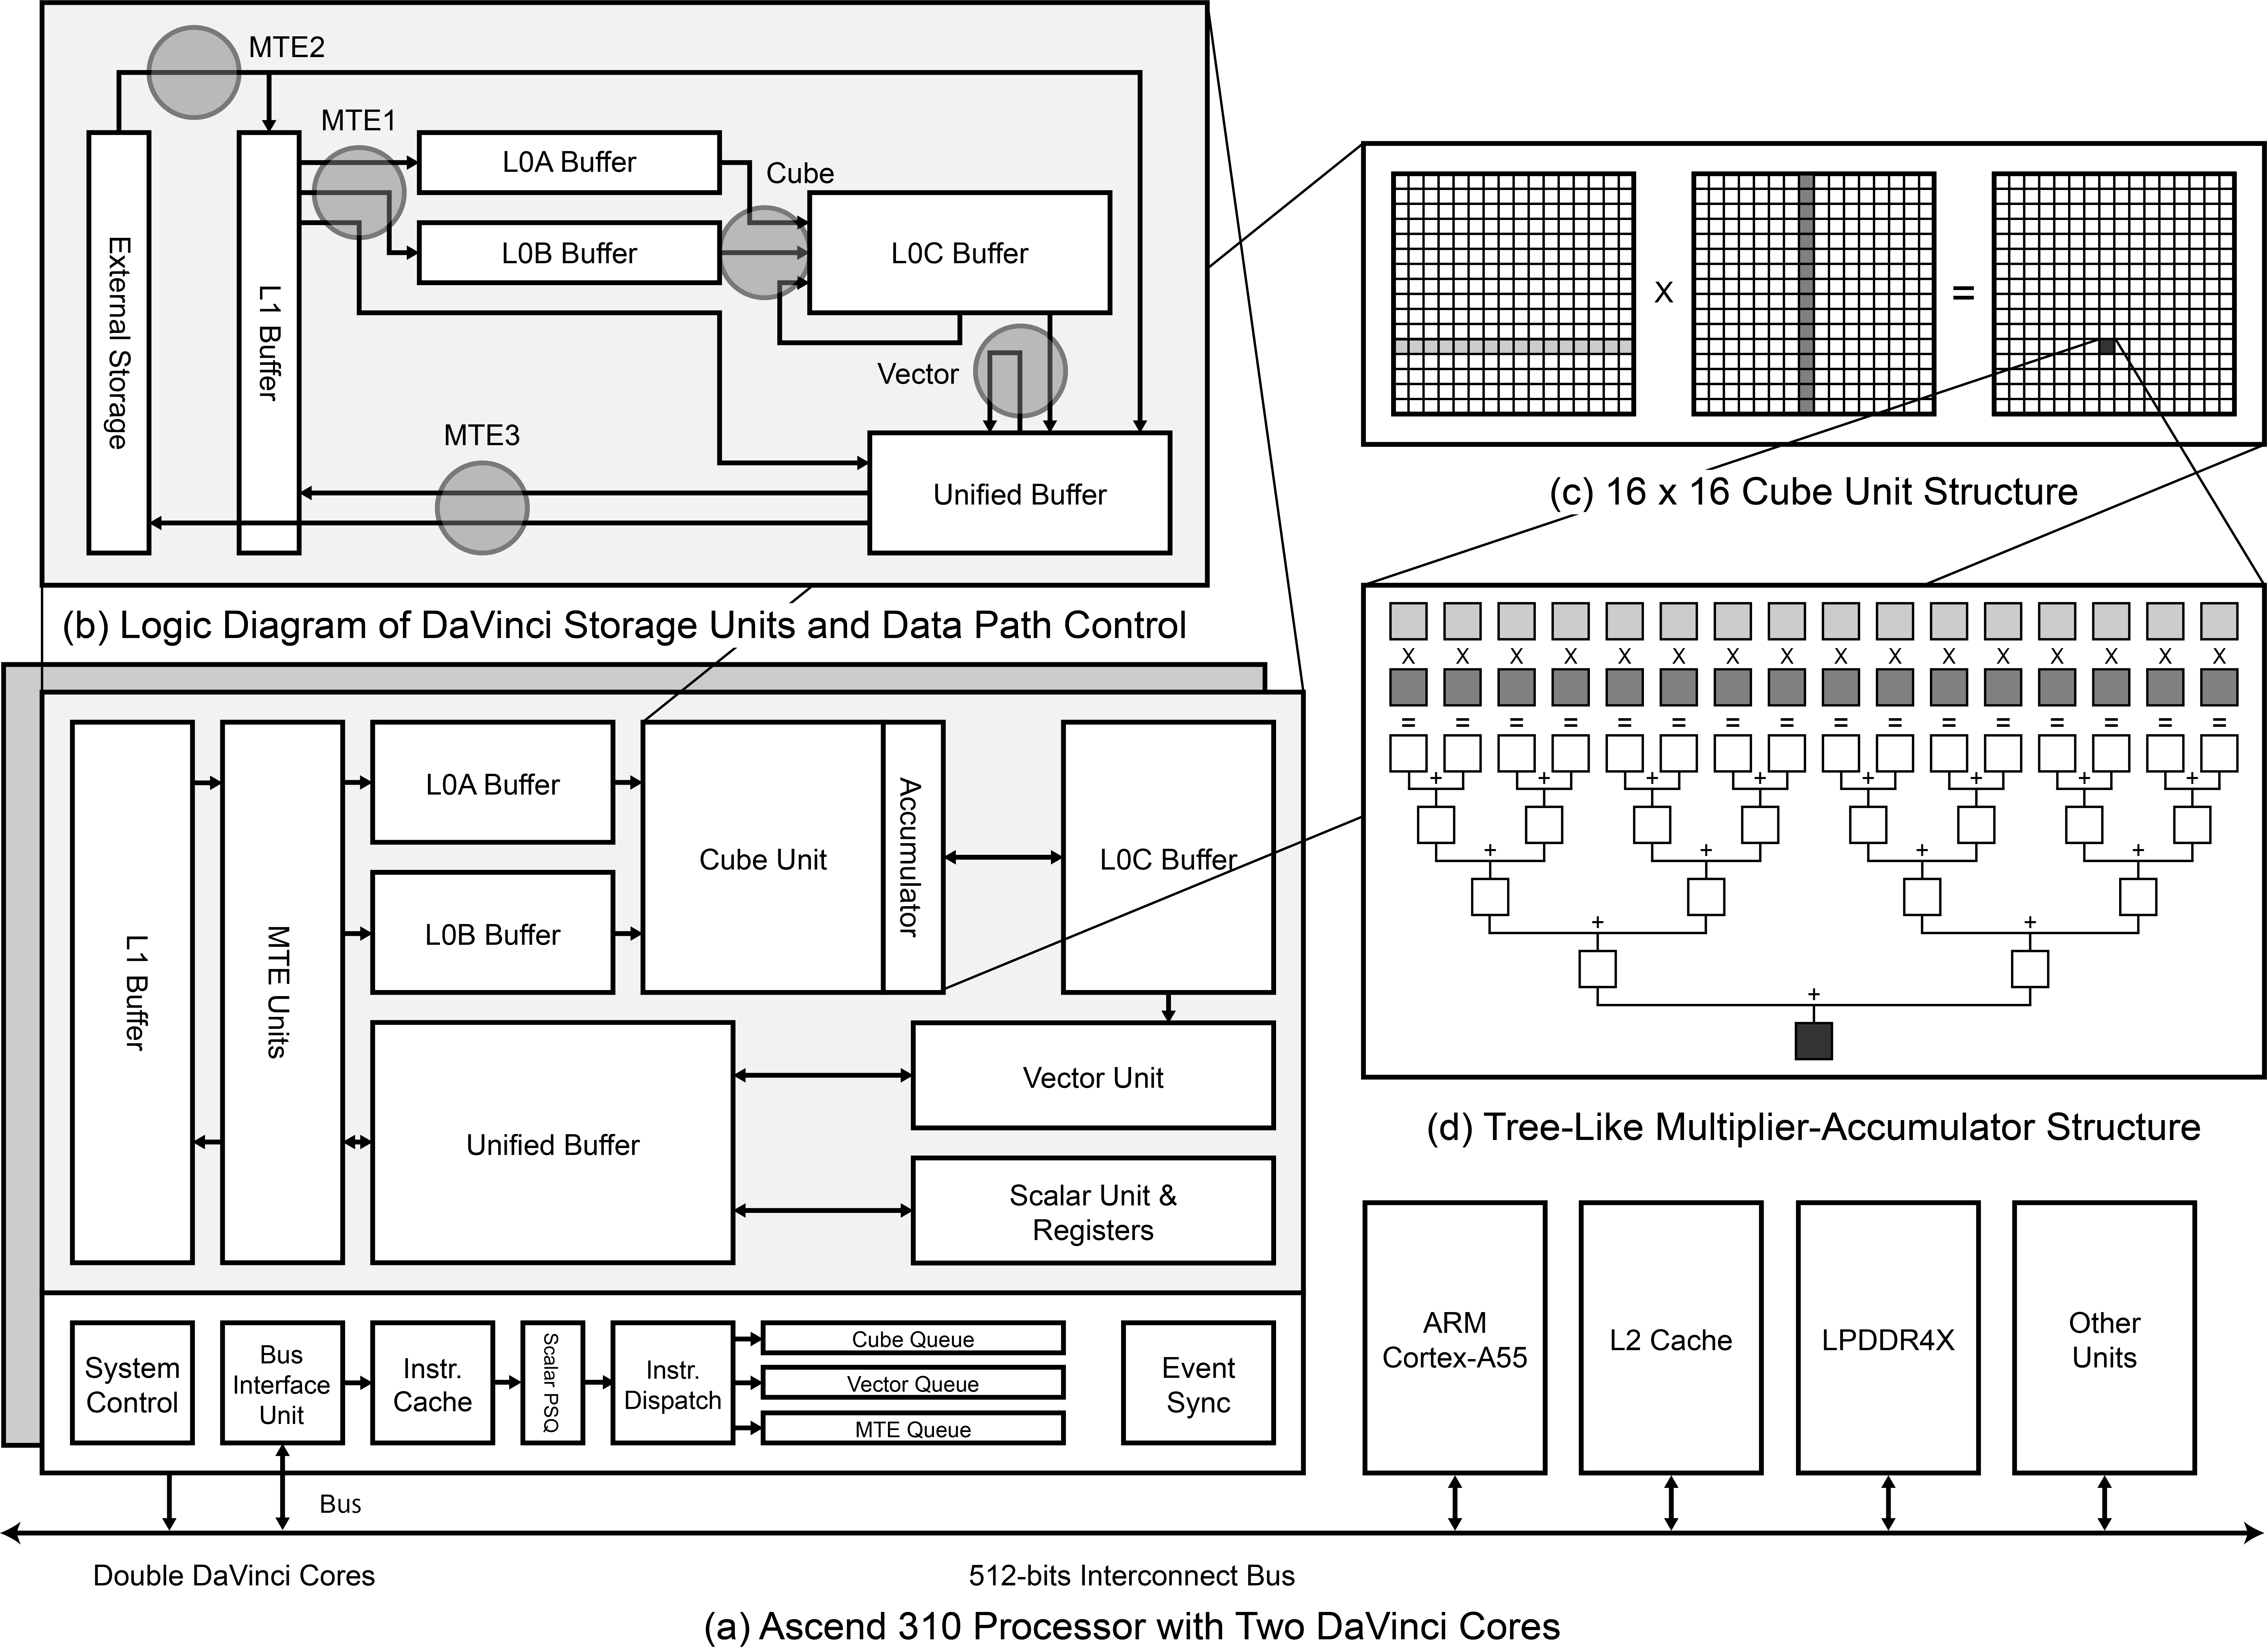
\includegraphics[scale=0.19]{figures/Ascend.png}}
    \caption{Overall Ascend 310 Structure. (a) Ascend 310 Processor with Two DaVinci Cores, (b) Logic Diagram of DaVinci Storage Units and Data Path Control, (c) 16 $\times$ 16 Cube Unit structure, (d) Tree-like Multiplier-Accumulator Structure (from \cite{DBLP:conf/hotchips/LiaoTXZ19})}
    \label{fig:dav}
    \end{figure}

The compute units include the Scalar Unit, Vector Unit, and Cube Unit. The Scalar Unit does mostly address calculations or condition branch analyses. The Vector Unit supports vectorized arithmetic or logical computations, including data preprocessing and activations. The Cube Unit is the essence of the DaVinci Core, improving the computation power of the matrix multiplications. A Cube Unit consists of 4096 FP16 MACs and 8192 INT8 MACs, forming $16 \times 16$ tree-like multiplier-accumulators, as shown in Fig. \ref{fig:dav} (c) (d). Each matrix multiplication is broken into multiple basic units of $16 \times 16 \times 16$ matrix multiplications. The accumulator behind the Cube Unit accumulates the intermediate results in the L0C Buffer.

The storage units refer to external storage, internal storage, and memory transfer units. The external storage includes L2 Buffer, DDR, and other storage devices accessed by the bus. The internal storage includes five memory buffers (L1, L0A, L0B, L0C, Unified Buffer) and registers. The Memory Transfer Engines (MTEs) control the data paths, which connect the internal storage buffers and transfer the data. The three MTEs (MTE1, MTE2, and MTE3) are tasked with the distinct data paths independently, as shown in Fig. \ref{fig:dav} (b). The five buffers and registers have different capacities and bandwidths, filling the gap between the low bandwidth and the high compute speed. 
    
The control units contain System Control, Scalar Program Scheduling Queue (PSQ), Instruction Dispatch, instruction queues (Cube Queue, Vector Queue, and three MTE Queues), and Event Synchronization. The Scalar PSQ receives and decodes the executing instructions from the Instruction Cache. After decoding, the Instruction Dispatch transmits the instructions to the queues separately. The Event Synchronization handles the data dependency among the units to ensure the correctness of execution orders, mainly a binary semaphore mechanism with eight registers. 

\subsection{Dissection and Optimization on AI processors}
\label{Sec:1_1_3}

With the growth of the AI processors, researchers paid high interest in this novel hardware with a lot of work in different areas. Similar to the previous works on regular GPUs \cite{DBLP:conf/ppopp/ZhangTXLZC17}, researchers have launched dissection works on the AI processors, e.g., the architecture of the Tensor Cores \cite{DBLP:journals/corr/abs-1804-06826}. Therefore, based on these dissections, some studies have been working on performance modeling on the AI processors. Their models can be divided into two categories: white-box hardware model \cite{DBLP:conf/ispass/RaihanGA19} and black-box statistics model \cite{DBLP:conf/nips/ChenZYJMCGK18, DBLP:journals/corr/abs-2008-01040}. The white-box hardware model requires a deep understanding of the hardware, which makes the model explainable but usually not general. Meanwhile, the black-box statistics model requires no hardware details but large scales of previous execution records for model training. 

In addition, more works focus on the optimization of the AI processors. At the level of the applications, studies focus on optimizing the original tasks of the AI processors, including the matrix multiplications \cite{DBLP:conf/ipps/00020C20} or the convolutions \cite{DBLP:conf/ppopp/YanWC20}. Other studies aim to extend the AI processors' computation power to more applications instead of deep learning only, including the Density-Based Spatial Clustering of Applications with Noise (DBSCAN) algorithm \cite{DBLP:conf/icpp/JiW21}, the basic operations of reduction and scan \cite{DBLP:conf/sccc/CarrascoVN18, DBLP:conf/ics/DakkakLXGH19}, skinny matrix multiplications \cite{DBLP:conf/ic-nc/TangK0K20}. Some other work even proposes next-generation AI processors, whose matrix MACs do general computations more than matrix multiplications \cite{10.1145/3470496.3527411}.

\section{Motivations}
\label{sec_1_2_motivations}

\subsection{Hidden Hardware Details of AI Processors}

Although hardware manufacturers have published various architectures of the AI processors, in addition to hardware parameters, the public and community are still unfamiliar with the hardware. One of the reasons is that most of those AI processors have no physical consumer-grade products but are only available on the cloud. Being affected by different sharing policies by virtual machines or containers, the benchmark performance cannot reflect the bare hardware performance as well as the details of the architecture. In addition, the toolchains of those AI processors are usually inadequate and only leave high-level abstraction APIs, primarily as operations in deep learning frameworks. Although the design allows the users to program without learning costs, it restricts them from analyzing the hardware and performing advanced hardware-ware optimization. Table \ref{tab:sec_1_2_table_1} reports the availability and API level of some popular AI processor manufacturers.

\begin{table}[tbp]
    \caption{Availability and API level of AI processor manufacturers}
    \label{tab:sec_1_2_table_1}
    \begin{center}
    
    \scalebox{0.85}{
        \begin{tabular}{c|c|c}
        \toprule[1pt]
            \textbf{Manufacturer} &
            \textbf{\makecell[c]{Public Availability}} &
            \textbf{API Level} \\
        \midrule[0.5pt]
    
        \makecell[c]{Qualcomm} &
        \makecell[c]{Mobile SOC \cite{HDSP}} &
        \makecell[c]{Operations in QNN \cite{QNN}}
        \\
        \midrule[0.5pt]
    
        \makecell[c]{Google} &
        \makecell[c]{Cloud platforms \cite{DBLP:conf/isca/JouppiYPPABBBBB17}} & 
        \makecell[c]{Operations in TensorFlow or \\ PyTorch XLA \cite{XLA}}
        \\
        \midrule[0.5pt]
    
        \makecell[c]{Cambricon} &
        \makecell[c]{Cloud platforms \cite{DevP}} &
        \makecell[c]{Low-level C \& assembly \cite{BANG}}
        \\
        \midrule[0.5pt]
    
        \makecell[c]{Nvidia} &
        \makecell[c]{Physical cards \cite{ADA}} &
        \makecell[c]{Low-level CUDA \& PTX \cite{PTX}}
        \\
        \midrule[0.5pt]
    
        \makecell[c]{Baidu} &
        \makecell[c]{Internal usage} &
        \makecell[c]{Applications in Baidu AI Cloud \cite{Pad}}
        \\
        \midrule[0.5pt]
    
        \makecell[c]{Huawei} &
        \makecell[c]{Physical cards \cite{DBLP:conf/hotchips/LiaoTXZ19}} &
        \makecell[c]{Low-level C \& assembly \cite{CANN}}
        \\
    
        \bottomrule[1pt]
        \end{tabular}
    }
    
    \end{center}
    \end{table}

Because of the restrictions above, in addition to the Nvidia GPUs, the hardware details of other AI processors are still hidden from the community. Therefore, the optimization works on the Nvidia GPUs \cite{DBLP:journals/corr/abs-1804-06826, DBLP:conf/ppopp/ZhangTXLZC17, DBLP:conf/ics/ZhouTZWS17, DBLP:conf/ispass/RaihanGA19, DBLP:conf/pldi/HongSKRKPRS18, DBLP:conf/cgo/ZhouMSM21} are significantly more than those on other AI processors. For hardware-aware algorithm optimizations on the AI processors, this thesis first performs a comprehensive dissection with various benchmarks on the AI processors.

\subsection{Inefficient Hardware Units on AI Processors \label{sec_1_2_2}}

\begin{figure}[tbp]
    \centering{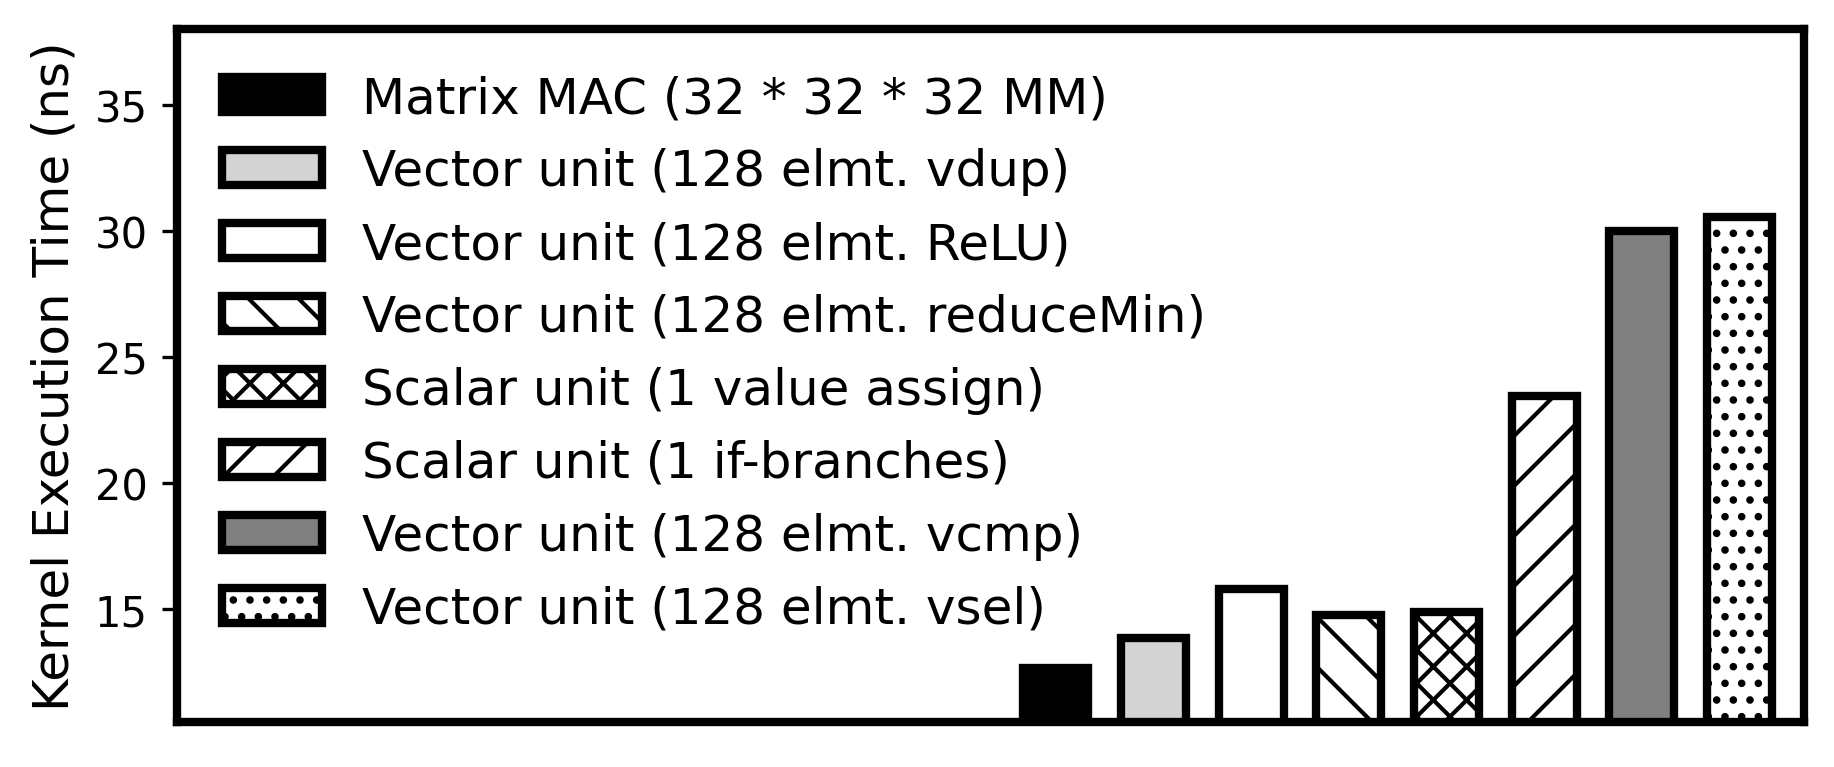
\includegraphics[scale=0.7]{figures/background_data.png}}
    \caption{The benchmark results on Huawei Ascend 310 AI processors}
    \label{fig:benchmark}
    \end{figure}

As independent processors, in addition to the Matrix MACs, the AI processors are equipped with other units for necessary operations, including instruction dispatching or vectorized computation. In addition, complete applications also consist of many of these operations, which sometimes occupy a significant part of execution. However, designers usually prefer assigning more hardware resources to enhance the performance of the matrix multiplications, leaving other units weakly supported \cite{DBLP:conf/icpp/JiW21, DBLP:conf/hotchips/LiaoTXZ19, DBLP:conf/isca/LiuDTHLXCC16, DBLP:conf/isca/JouppiYPPABBBBB17, cambricon, CANN, jax}. 

On the Huawei Ascend 310 AI processor, we offer an instruction-level benchmark, where we duplicate the operations and fit the execution time with the least square method. Fig. \ref{fig:benchmark} shows that a scalar single-operand conditional branch takes an average of 1.48$\times$ longer than \verb|ReLU|, 1.69$\times$ longer than \verb|vecDup|, 1.60$\times$ longer than \verb|reduceMin| on 128 elements in parallel. An immediate assignment to on-core memory takes 0.94$\times$ of \verb|ReLU|, where \verb|ReLU| consists of data reading, computation, and data writing. The vectorized comparisons \& selections take 1.90$\times$ and 1.93$\times$ than \verb|ReLU| respectively, showing lower performance. The hardware features restrict the implementation of classical algorithms from other platforms. Even after successful migrations, the algorithms could face heavy performance loss.

\subsection{Low Usage Rate of Matrix MACs}

Since the matrix MACs of the AI processors compute matrix multiplications only, most algorithms or applications cannot utilize the high-performance matrix MACs. Even for the matrix multiplication itself, the usage rate of the matrix MACs is far lower than expected. Fig. \ref{fig:low_usage} illustrates the hardware unit usage rates of a standard matrix multiplication implementation on the Huawei Ascend 310 processors. The results show that the IO units report significantly higher usage rates than the matrix MACs, even when the IO part of the matrix multiplication is $O(n^2)$ and the core matrix multiplication is $O(n^3)$.

\begin{figure}[tbp]
    \centering{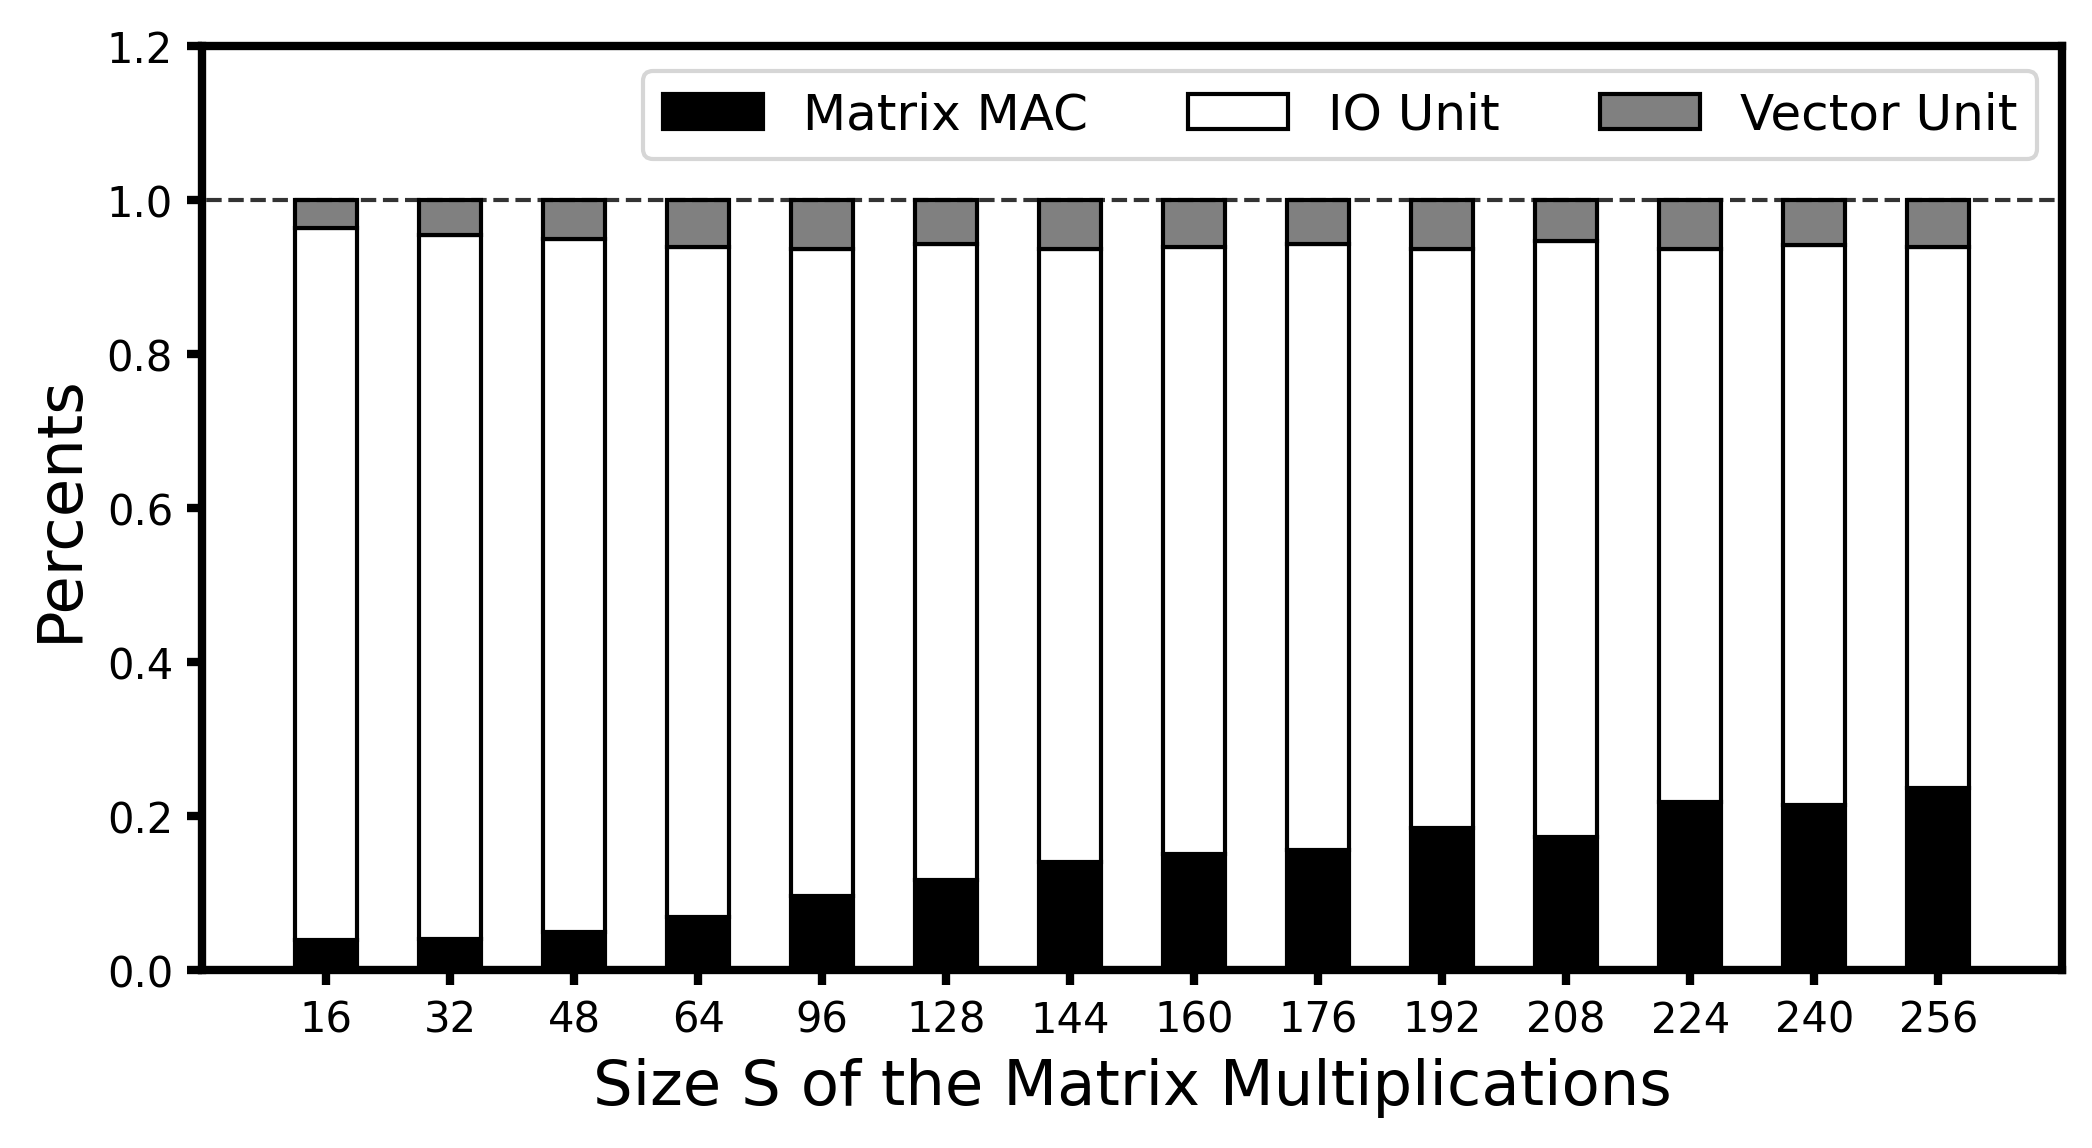
\includegraphics[scale=0.7]{figures/low_usage.png}}
    \caption{Unit Usage Rates of Matrix Multiplications $S \times S \times S$ on Huawei Ascend 310 AI processors}
    \label{fig:low_usage}
    \end{figure}

As discussed in Sec. \ref{Sec:1_1_3}, researchers have been working on the programmability of the AI processors. The primary idea for their work is to adapt the classical algorithms for matrix MACs, which also aims to improve the usage rates of the matrix MACs.

\section{Main contributions}
\label{sec_1_3_contributions}

\subsection{Performance Modeling on Huawei Ascend}

We first demystify the Huawei Ascend 310 with micro-benchmarks to show the characteristics of the hardware units on DaVinci Core, the AI Core of the Huawei Ascend processor. We pay the most attention to the IO units, which play the most critical role and influence the execution time, as shown in Fig. \ref{fig:low_usage}. We reveal how MTE Units control and compete for the data paths that connect the different separate memories. In addition to the contention ratio benchmark on bandwidth sharing, we design specially-crafted benchmarks to identify the source, which is asserted to be the Interconnect Bus, and the runtime behaviors of the bus contention.

Then, we propose a discrete-event-based performance model, \textbf{Verrocchio}. Verrocchio models a series of architectural features that are most important and determinant for the DaVinci Core performance, including bandwidth contentions and concurrent hardware unit execution with synchronization. The evaluation results show that Verrocchio achieves an average error rate of $2.62\%$ and $2.30\%$ for the single-core and double-core execution of several sample kernels. We demonstrate the use of Verrocchio in optimizing a matrix multiplication algorithm. Verrocchio enables a search space exploration in tiling size selection and achieves a speedup of 1.70$\times$ at the operator level and 1.53$\times$ at the application level compared with CANN \cite{CANN} native operators with prediction error rates of $5.06\%$ and $5.25\%$ for the single-core and double-core execution.

\subsection{1) Replacing the Worst Operations}

\textbf{SelB-\textit{k}-NN} (\textbf{Sel}ection-\textbf{B}itonic-\textbf{\textit{k}}-\textbf{NN}) is a mini-batch \textit{k}-NN for the powerful AI processors. For a single batch, SelB-\textit{k}-NN includes a naturally-accelerated distance computation and a non-trivial \textit{k}-selection. For the \textit{k}-selection, inspired by the selection sort, SelB-\textit{k}-NN compares the minimized value of the distance computation results with the first element of the min-\textit{k} result array, maintained by the bitonic 1-selection \cite{DBLP:conf/sigmod/ShanbhagPM18}. Compared with the previous approaches, SelB-\textit{k}-NN limits the increment of the weakly-supported scalar operations, vectorized comparisons \& selections. Since the architectures and instruction sets of the AI processors vary among manufacturers, we propose two algorithms to minimize the hardware support requirements for better portability. As a result, only \verb|vecDup|, \verb|ReLU|, and \verb|reduceMin| (\verb|reduceMax|) with no indexing are sufficient, which contribute to the most significant and necessary operators on most AI processors. For all mini-batches, an early exit policy dynamically reduces most of the \textit{k}-selection workloads, which our quantification shows shrink in an inverse proportion. We model the tiling shape selection to an optimization problem, considering the overall performance of SelB-\textit{k}-NN. In addition, we propose an offline pruning method working during preprocessing to reduce the optimization problem's search space.

\subsection{2) Transforming to Matrix Multiplications}

\textbf{Cube-}$\mathbf{f(x)}$ leverages the computational power of the Matrix MACs on AI processors to evaluate special functions with the Taylor polynomials. Cube-${f(x)}$ treats the building and computation of Taylor polynomials as specific cases of matrix multiplications, which are efficiently accelerated by the Matrix MACs. Cube-${f(x)}$ has two stages: preparation and computation. In the preparation stage, Cube-${f(x)}$ generates a variable sequence $(x^{k_0}, x^{k_1}, x^{k_2}, ...)$ as the variables of the Taylor polynomials. In the computation stage, Cube-${f(x)}$ evaluates multiple independent special functions by reusing the variable sequence generated by the preparation stage with different coefficients in parallel. Depending on different precision requirements, Cube-${f(x)}$ applies a required order of expansion to approximate the original functions. When given a low order requirement, Cube-${f(x)}$ achieves data parallelism with a novel technology named In-matrix Parallelism. By adjusting the inputs of the matrix multiplications, it merges multiple input vectors and computes within one matrix multiplication instruction. Since In-matrix Parallelism cannot always improve the efficiency of Cube-${f(x)}$, we formulate an optimization problem, which minimizes the algorithm execution time by searching for the best number of inputs being merged. Compared with previous approaches, Cube-${f(x)}$ significantly reduces the vector operations, which perform weakly on the AI processors, reuses the intermediate results, and migrates most of the computation to the Matrix MACs by doing special cases of matrix multiplications.

\section{Thesis Organization}
\label{sec_1_4_organization}

TODO

%========================================

\chapter{Performance Modeling on Huawei Ascend}
\label{sec_2}

\section{Verrocchio, A Performance Model}
\label{sec_2_1}

The specific hardware structure of the DaVinci Core, discussed in Sec. \ref{Sec:1_1_2}, guarantees high performance for AI applications while leaving several challenges for performance modeling and further optimization. This section first discusses the key challenges we address, how to model the storage unit hardware performance and the concurrent execution synchronization. Then we give an overview of our performance model, Verrocchio, which aims to overcome the challenges for accurate performance modeling.

\subsection{Key Challenges}

\subsubsection{Storage Unit Hardware Performance}

Since different MTE Units control different data paths, the bandwidth of each path requires benchmarking respectively. Especially, multiple MTE Units are allowed to share a single data path concurrently, which would bring bandwidth contentions and significantly influence the hardware performance. As shown in Fig. \ref{fig:dav} (a), the data path controlled by the on-core bus is the only access for the DaVinci Cores to the off-core 512-bits Interconnect Bus. Fig. \ref{fig:dav} (b) illustrates that the MTE2 and MTE3 Units both transfer data between the external storage and the DaVinci Core. The architecture suggests a potential contention between the MTE2 and MTE3 Units. However, from the figure of the hardware structure, we cannot postulate the existence of the contention and figure out the contention source: the MTE Units, the on-core bus unit, or the off-core Interconnect Bus. Without the knowledge of the source, simply fitting the performance of the contentions could be inappropriate.

Furthermore, existing studies on the hardware resource contentions \cite{DBLP:conf/sc/HristeaLK97, DBLP:conf/usenix/SrikanthanDS15} mainly focus on the performance variations caused by the different contention ratios when the bandwidths are saturated. In addition to the analyses of the contention ratio, the benchmark of the MTE Unit contention in our performance modeling should pay further attention to the entire runtime of the contention and not only to the stable saturated status. One of the most common methods to monitor the entire runtime of a kernel is sampling \cite{IBM_profiler, Del_profiler, Goo_profiler}. However, since the DaVinci Cores have no breakpoint or in-kernel timestamp mechanism, we can hardly insert sampling points into the DaVinci kernels. Therefore, designing a benchmark to measure the runtime of the contention becomes a challenge.

\subsubsection{Concurrent Execution and Synchronization}

\begin{figure}[htbp]
    \begin{adjustbox}{addcode={\begin{minipage}{\width}}
        {\end{minipage}},rotate=90,center}
        \begin{minipage}[b]{\textheight}
            \centering
            \subfigure{} {
                \begin{adjustbox}{addcode={\begin{minipage}{\textheight}}
                    {\caption{The DaVinci Core working details}
                    \label{fig:soft}
                    \end{minipage}},center}
                    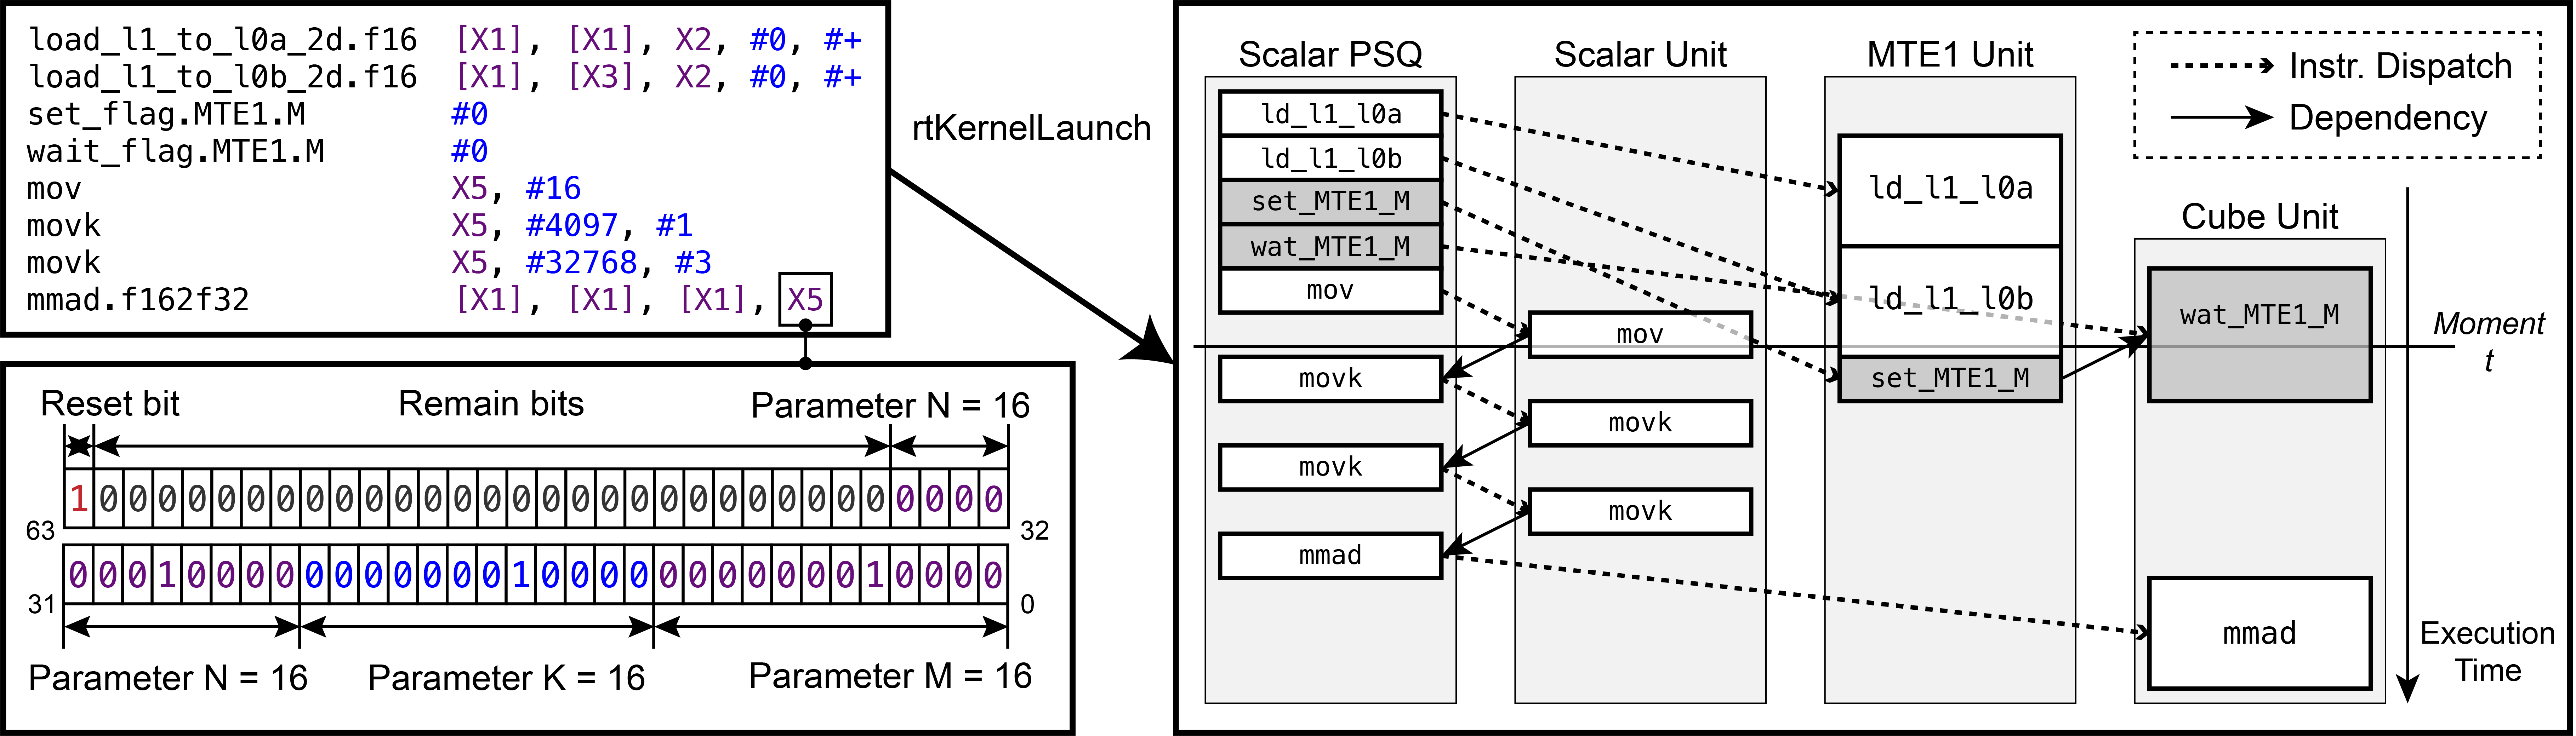
\includegraphics[scale=0.30]{figures/reduced_soft.png}
                \end{adjustbox}       
            }\\
            \centering
            \subfigure{} {
                \begin{adjustbox}{addcode={\begin{minipage}{\textheight}}
                    {\caption{The examples of kernels influenced by the binary semaphore}
                    \label{fig:instr}
                    \end{minipage}},center}
                    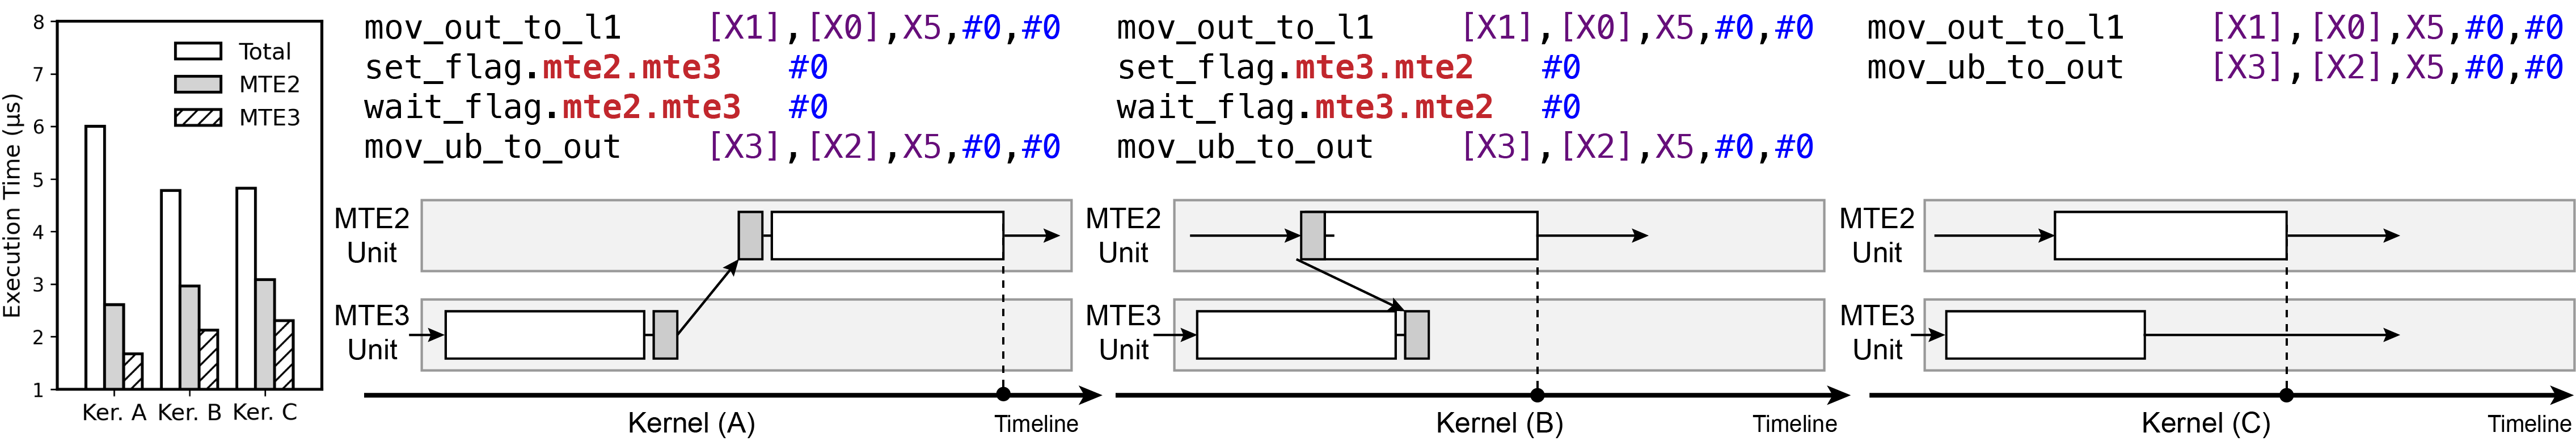
\includegraphics[scale=0.48]{figures/mov_test.png}
                \end{adjustbox}        
            }
        \end{minipage}      
    \end{adjustbox}
\end{figure}

\begin{figure}[htbp]
\end{figure}

As we demystify in Fig. \ref{fig:soft}, all the instruction queues, including the Scalar PSQ, strictly follow the FIFO policy. The Scalar PSQ maintains input kernel instructions and identifies the type of each instruction (Scalar, Vector, Cube, MTE1/2/3), which performs as Instruction Decoder in CPUs. The types of instruction determine the instruction queue to which the instruction is sent, as well as the concurrent unit on which the instruction is executed. For the Scalar instructions, the Scalar PSQ directly sends them to the Scalar Unit. For others, the Scalar PSQ sends them to the corresponding instruction queues via Instruction Dispatch. Each compute or storage unit executes one single instruction at every moment. When a unit is idle, the corresponding queue dequeues the oldest instruction to the unit for execution. The Scalar PSQ asynchronously dispatches the instructions except for the Scalar instructions.

While the DaVinci Core adopts the single-thread execution model, the concurrency of the hardware units makes the Instruction-Level Parallelism (ILP) supported. To guarantee the dependency among the units, the programmers must manually insert the \verb|set_flag| and \verb|wait_flag| instructions, acting as the binary semaphore mechanism. 
The fundamental operations of the semaphore mechanism are PV Operations \cite{EWD:EWD74}. P Operation decrements the value of the semaphore variable by 1. If the new variable is negative, it blocks the caller process. Meanwhile, V Operation increments the value of the semaphore variable by 1. If the old variable is negative, it wakes up a blocked process and lets it access a resource unit. 
In DaVinci Cores, the \verb|wait_flag| acts as P Operation and the \verb|set_flag| performs as V Operation. The Scalar PSQ assigns the two semaphore operations to the corresponding instruction queue just as it does with other instructions. In the example of the moment \verb|t|, following the FIFO policy, the \verb|set_flag| (\verb|set_MTE1_M|) in the MTE1 queue shall not start due to the incompleteness of the last instruction \verb|ld_l1_l0b|. The corresponding \verb|wait_flag| (\verb|wat_MTE1_M|) keeps blocking the Cube Unit until the execution of \verb|set_flag|. Therefore, the instruction \verb|mmad| shall not start before the end of the \verb|ld_l1_l0b|.

\begin{figure}[htbp]

\end{figure}

The idleness of the hardware unit caused by the synchronization is one of the most critical factors influencing the execution time. Each instruction could prolong or block the execution based on its programming logic. Furthermore, the concurrent execution can be intentionally activated or deactivated, which is decided by how the kernel programs schedule the multiple semaphore registers and control flows. Fig. \ref{fig:instr} illustrates a simple DaVinci kernel containing two data transfer operations (on MTE2 and MTE3 Units) with different binary semaphore operations. As a result, Kernel (A) takes 1.26$\times$ more time than Kernel (B) and 1.24$\times$ more than Kernel (C), while the actual two data transfer operations take similar time among all kernels. 
For Kernel (A) and Kernel (B), the parameter order (\verb|mte2.mte3| \& \verb|mte3.mte2|) of the semaphore operations determines the execution time. The parameter order \verb|mte2.mte3| prohibits the concurrent execution while the reversed \verb|mte3.mte2| does not, which reports a similar result to Kernel (C).
Therefore, the DaVinci Core working details make the modeling methods based on kernel metadata analysis or statistics ineffective, e.g., the most straightforward execution time computed by $DataSize / Bandwidth$. From the view of those modeling methods without analysis in the instruction logic, Kernel (A) and (B) should have a similar total execution time, which is false in our evaluations. Then it is necessary to model the performance with the instruction-level analyses in the kernel source codes.

\subsection{Overview of Verrocchio}

\begin{figure}[htbp]
    \begin{adjustbox}{addcode={
        \begin{minipage}{\width}}{
            \caption{Verrocchio, a discrete-event-based performance model}
            \label{fig:over}
        \end{minipage}},rotate=90,center}
        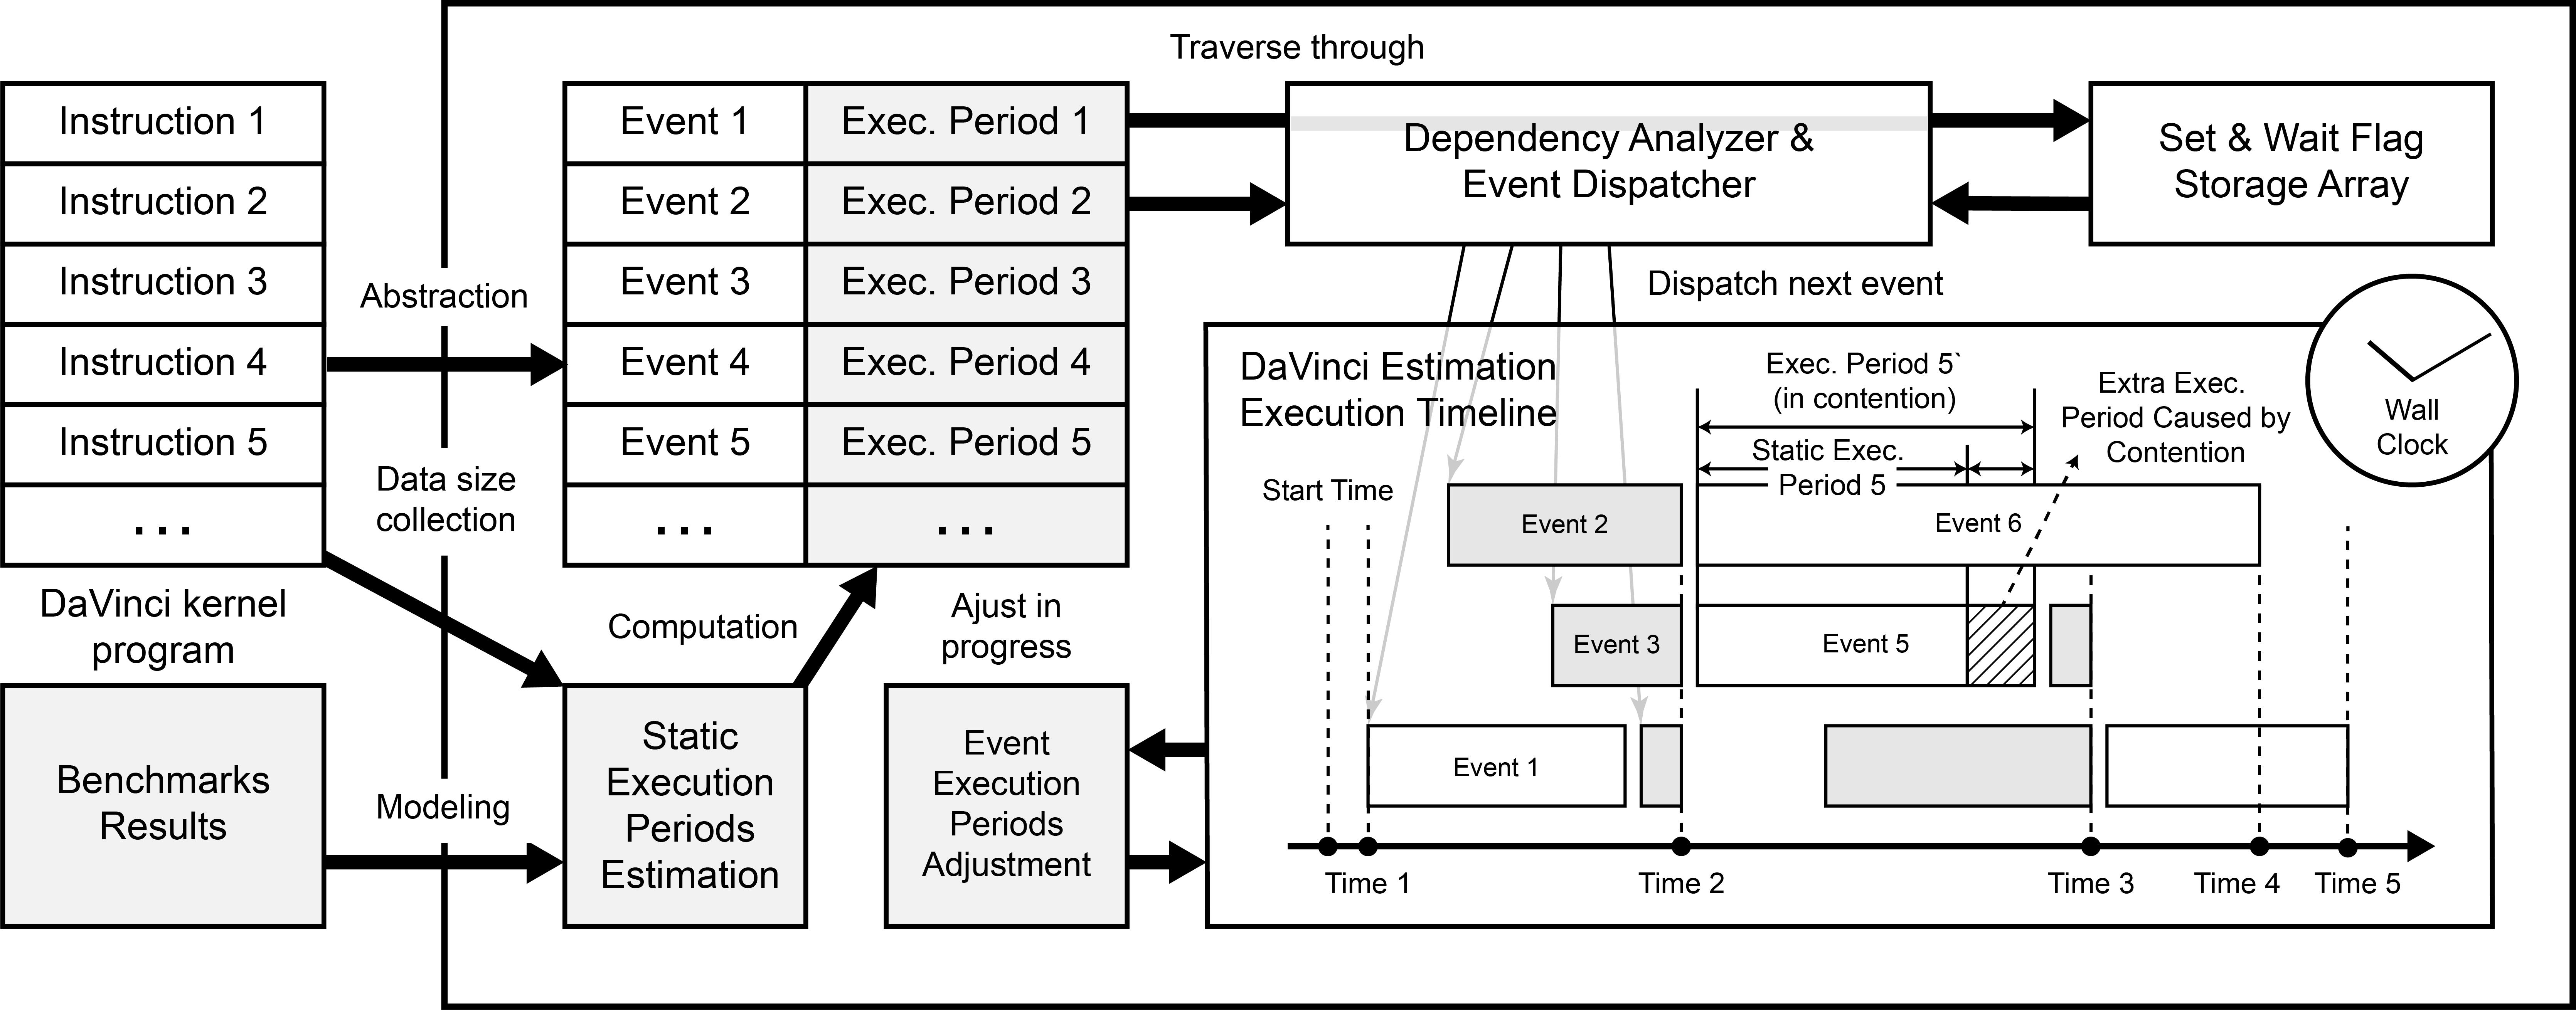
\includegraphics[scale=0.33]{figures/overview.png}
    \end{adjustbox}
\end{figure}

Verrocchio is a discrete-event-based performance model, where events occur due to occurrence time with execution periods at the discrete points in time. Fig. \ref{fig:over} illustrates the structure of our DaVinci Core model. Verrocchio has two inputs, the target program source codes and the hardware benchmark results. It predicts and outputs the execution period of the kernel program.

To provide instruction-level modeling for the kernel program, Verrocchio first scans the instructions of the kernel program to abstract them into discrete events. It also collects the data size for each instruction. Verrocchio applies the results from our instruction-level micro-benchmarks, which target to expose the hardware performance, especially the DaVinci Core storage unit performance. Combining the data size and the benchmark results, Verrocchio estimates the static execution period of each instruction, which is the execution period when the instruction executes alone.

Two core components of Verrocchio are the dependency analyzer and event dispatcher, which manage the prepared discrete events and place them on a DaVinci execution timeline at the correct timestamp with a wall clock. To handle the synchronization supported by the binary semaphore, Verrocchio maintains two arrays from the analysis of the prepared events. The two sorted arrays store the Set Flag and Wait Flag operations and guide Verrocchio correctly start an event when meeting the binary semaphore conditions. As we discussed, during the procedure, the event execution periods can be updated because of the bandwidth contention, as the example of Event 5 shown in Fig. \ref{fig:over}. To model the contentions, Verrocchio offers the execution periods adjustment, which updates the new execution periods each time the contentions begin and end.

\section{Benchmarking DaVinci}

To reveal the performance of the storage unit, we benchmark the Ascend 310 processor by launching a series of instruction-level micro-benchmarks. For the hardware units, whose performance reports a regular and stable trend, the benchmark increases the processed data size and computes the bandwidth by the least-square method. For the bus bandwidth, which connects to the external storage and involves the contention by the MTE2 and MTE3 Units, we first design a specifically-crafted benchmark to identify the contention source and expose the runtime behaviors. Then we adopt further benchmarks with different contention ratios to quantify the bandwidth sharing under contentions.

\subsection{Benchmarks for Hardware Units \label{sec:cube_bench}}

\subsubsection{Methodology}

For the MTE1 Unit, we directly adopt the micro-benchmark kernels. For the Vector Unit, we list the data movement bandwidth here and with a precision converting function from FP32 to FP16. For the Cube Unit, we benchmark the FLOPS by modifying the \verb|mmad| instruction parameters. The computation amount of each minimized $16 \times 16 \times 16$ matrix multiplication is $(15 + 16) \times (16 \times 16) = 7936$ FLOPs. After the single-core benchmarks, we activate and benchmark two DaVinci Cores on the Ascend 310 processor. We compare the results with the single-core results to check whether the double-core execution can approximately double the bandwidths or FLOPSs. In addition, we also benchmark the kernel launch time of double-core execution compared with the single-core execution. 

\subsubsection{Benchmark Results} 

\begin{table}[tbp]
    \caption{Ascend 310 Cube Unit benchmark results}
    \label{tab:bench}
    \begin{center}
    \scalebox{0.73}{
        \begin{tabular}{c|c|c|c}
        \toprule[1pt]
        \textbf{Benchmark Types} & \textbf{Double-Core} & \textbf{Single-Core} & \textbf{Percentages} \\
        \midrule[0.5pt]
        MTE1 bw. (L1 Buffer to L0A Buffer) & 695.97 GB/s & 347.99 GB/s & 99.99\% \\
        MTE1 bw. (L1 Buffer to L0B Buffer) & 348.79 GB/s & 174.37 GB/s & 100.00\% \\
        Vector bw. (None) & 348.16 GB/s & 174.06 GB/s & 100.00\% \\
        Vector bw. (F32 to F16) & 348.2 GB/s & 174.09 GB/s & 100.00\% \\
        \midrule[0.5pt]
        Cube Unit practical FLOPS (RESET off) & 10796.92 GFLOPS & 5390.32 GFLOPS & 100.00\% \\
        Cube Unit practical FLOPS (RESET on) & 10789.17 GFLOPS & 5397.34 GFLOPS & 99.99\% \\
        Ascend 310 documented FLOPS & - & 4096.00 GFLOPS & - \\
        \midrule[0.5pt]
        Kernel launch time & 2293.5 ns & 2354.5 ns & - \\
        \bottomrule[1pt]
        \end{tabular}
    }
    \end{center}
    \end{table}


We list the benchmark results in Table \ref{tab:bench}. We summarize two main observations of the results as follows:

\begin{itemize}
    \item As we expected, the independent hardware units report perfectly double acceleration. These hardware units require on-core resources only (bandwidths and computation power) and shall not suffer performance loss in the multi-core execution situation because of the Interconnect Bus.
    
    \item The kernel launch time results report that the double-core execution shows no apparent kernel launch time extension compared with the single-core execution. We assert that the kernel launch time does not suffer from any contentions in double-core execution. As DaVinci Cores have no inter-core communication mechanism, we assume that the two DaVinci Cores on Ascend 310 processors start and execute the kernel synchronically.
\end{itemize}


\subsection{Benchmarks for Bus Contention Source and Runtime Behaviors}

While the bandwidth of the individual bus execution can be evaluated naturally with the benchmark in Sec. \ref{sec:cube_bench}, the contention caused by the multiple units is non-trivial to be measured. In this subsection, we design a benchmark to study the source and the runtime behaviors of the contentions observed at the DaVinci Cores bus, which are caused by the MTE2 and MTE3 Units. 

\subsubsection{Benchmark Design \label{sec:ben_des}}

\begin{figure}[tbp]
    \centering{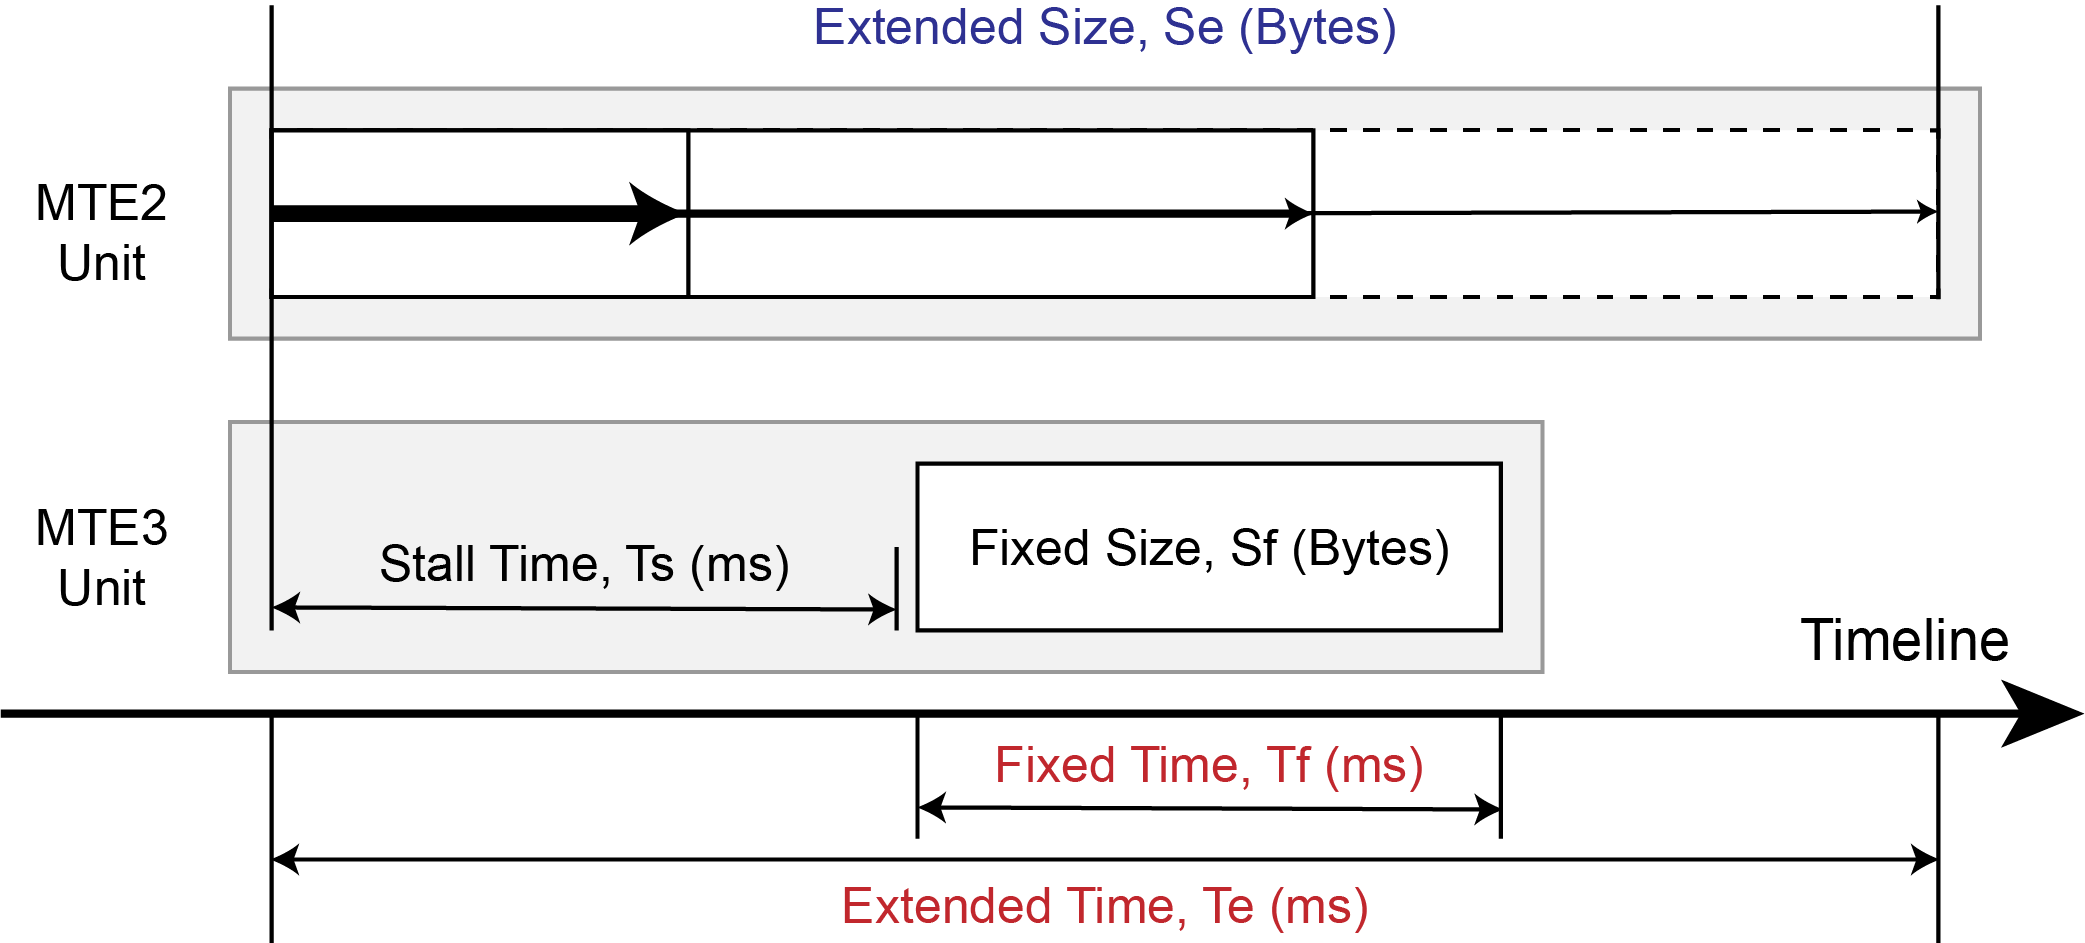
\includegraphics[scale=0.55]{figures/bench_meth.png}}
    \caption{Bandwidth contention monitoring benchmark (e.g., MTE2 \& MTE3 Units)}
    \label{fig:bench_meth}
    \end{figure}


\begin{algorithm}[tbp]
    \caption{Bandwidth Contention (e.g., MTE2 \& MTE3 Units)}
    \label{alg:bench_meth}
        
    \SetKwInOut{Input}{input}
    \SetKwInOut{Output}{output}
        
    \BlankLine
    \Input{
        Stall time, $T_{s}$; Fixed size, $S_{f}$
    }
            
    \Output{
        Extended time array: $A_{e}$; Fixed time array: $A_{f}$
    }
    \BlankLine

    \For{$Se : 0 \to $ MAX}{
        \textbf{Barrier call} \\
        \textbf{(MTE2)} Process data of size $S_{e}$ \\
        \textbf{(Scalar)} Dummy instruction \\
        \textbf{(Scalar)} $\cdots$ $\cdots$ \  (Block instruction 7 for $T_{s}$)\\
        \textbf{(Scalar)} Dummy instruction \\
        \textbf{(MTE3)} Process data of size $S_{f}$ \\
    }
\end{algorithm}

The objective of the benchmark is to monitor the behaviors of the entire contention runtime, from the start to the end of it, with a fixed contention ratio of two (the MTE2 and MTE3 Units). 
As shown in Fig. \ref{fig:bench_meth},
on one of the hardware units (e.g., the MTE2 Unit), we first let the unit process an increasing size of data, $S_{e}$, and then keep it idle until the end. For the other hardware unit (e.g., the MTE3 Unit), which is concurrently executing alongside, it first stays idle for a short period $T_{s}$ and then processes a segment of data with the size of $S_{f}$ until the end. 
On the DaVinci Cores, we insert dummy Scalar instructions between the instructions of the former unit and the latter, as annotated in Alg. \ref{alg:bench_meth}. 
As discussed, the Scalar PSQ must wait until the end of the Scalar instructions and proceed to the next instruction. Therefore, the dummy instructions block the Scalar PSQ and keep the latter unit idle. When the former unit has been executing for a period, the latter unit finally receives its instruction from the Scalar PSQ and then executes with the designed contention. We measure and record the execution time of two units, $T_{e}$ and $T_{f}$ with the Huawei official profiler respectively, with the increment of $S_{e}$.

Divided by $T_{e}$, the two hardware units experience three contention statuses: before, under, and after contention. When $T_{e} < T_{s}$, where $S_{e}$ is not large enough, the two hardware units stay the status before contention. When $T_{e} < T_{s} + T_{f}$, the two units are under contention. When $T_{e} > T_{s} + T_{f}$, the two units finish the contention periods at the status after contention. Therefore, after finishing the benchmark in Alg. \ref{alg:bench_meth}, the recorded execution time $T_{e}$ and $T_{f}$ can expose the entire runtime behaviors during the bandwidth contention. In addition, we vary the input parameters $T_{s}$ and $S_{f}$ to study the potential influences by the contention beginning time and processed data size under contention.

\subsubsection{Contention Source and Runtime Behavior Results \label{sec:runtime}}

\begin{figure}[t]
    \centering{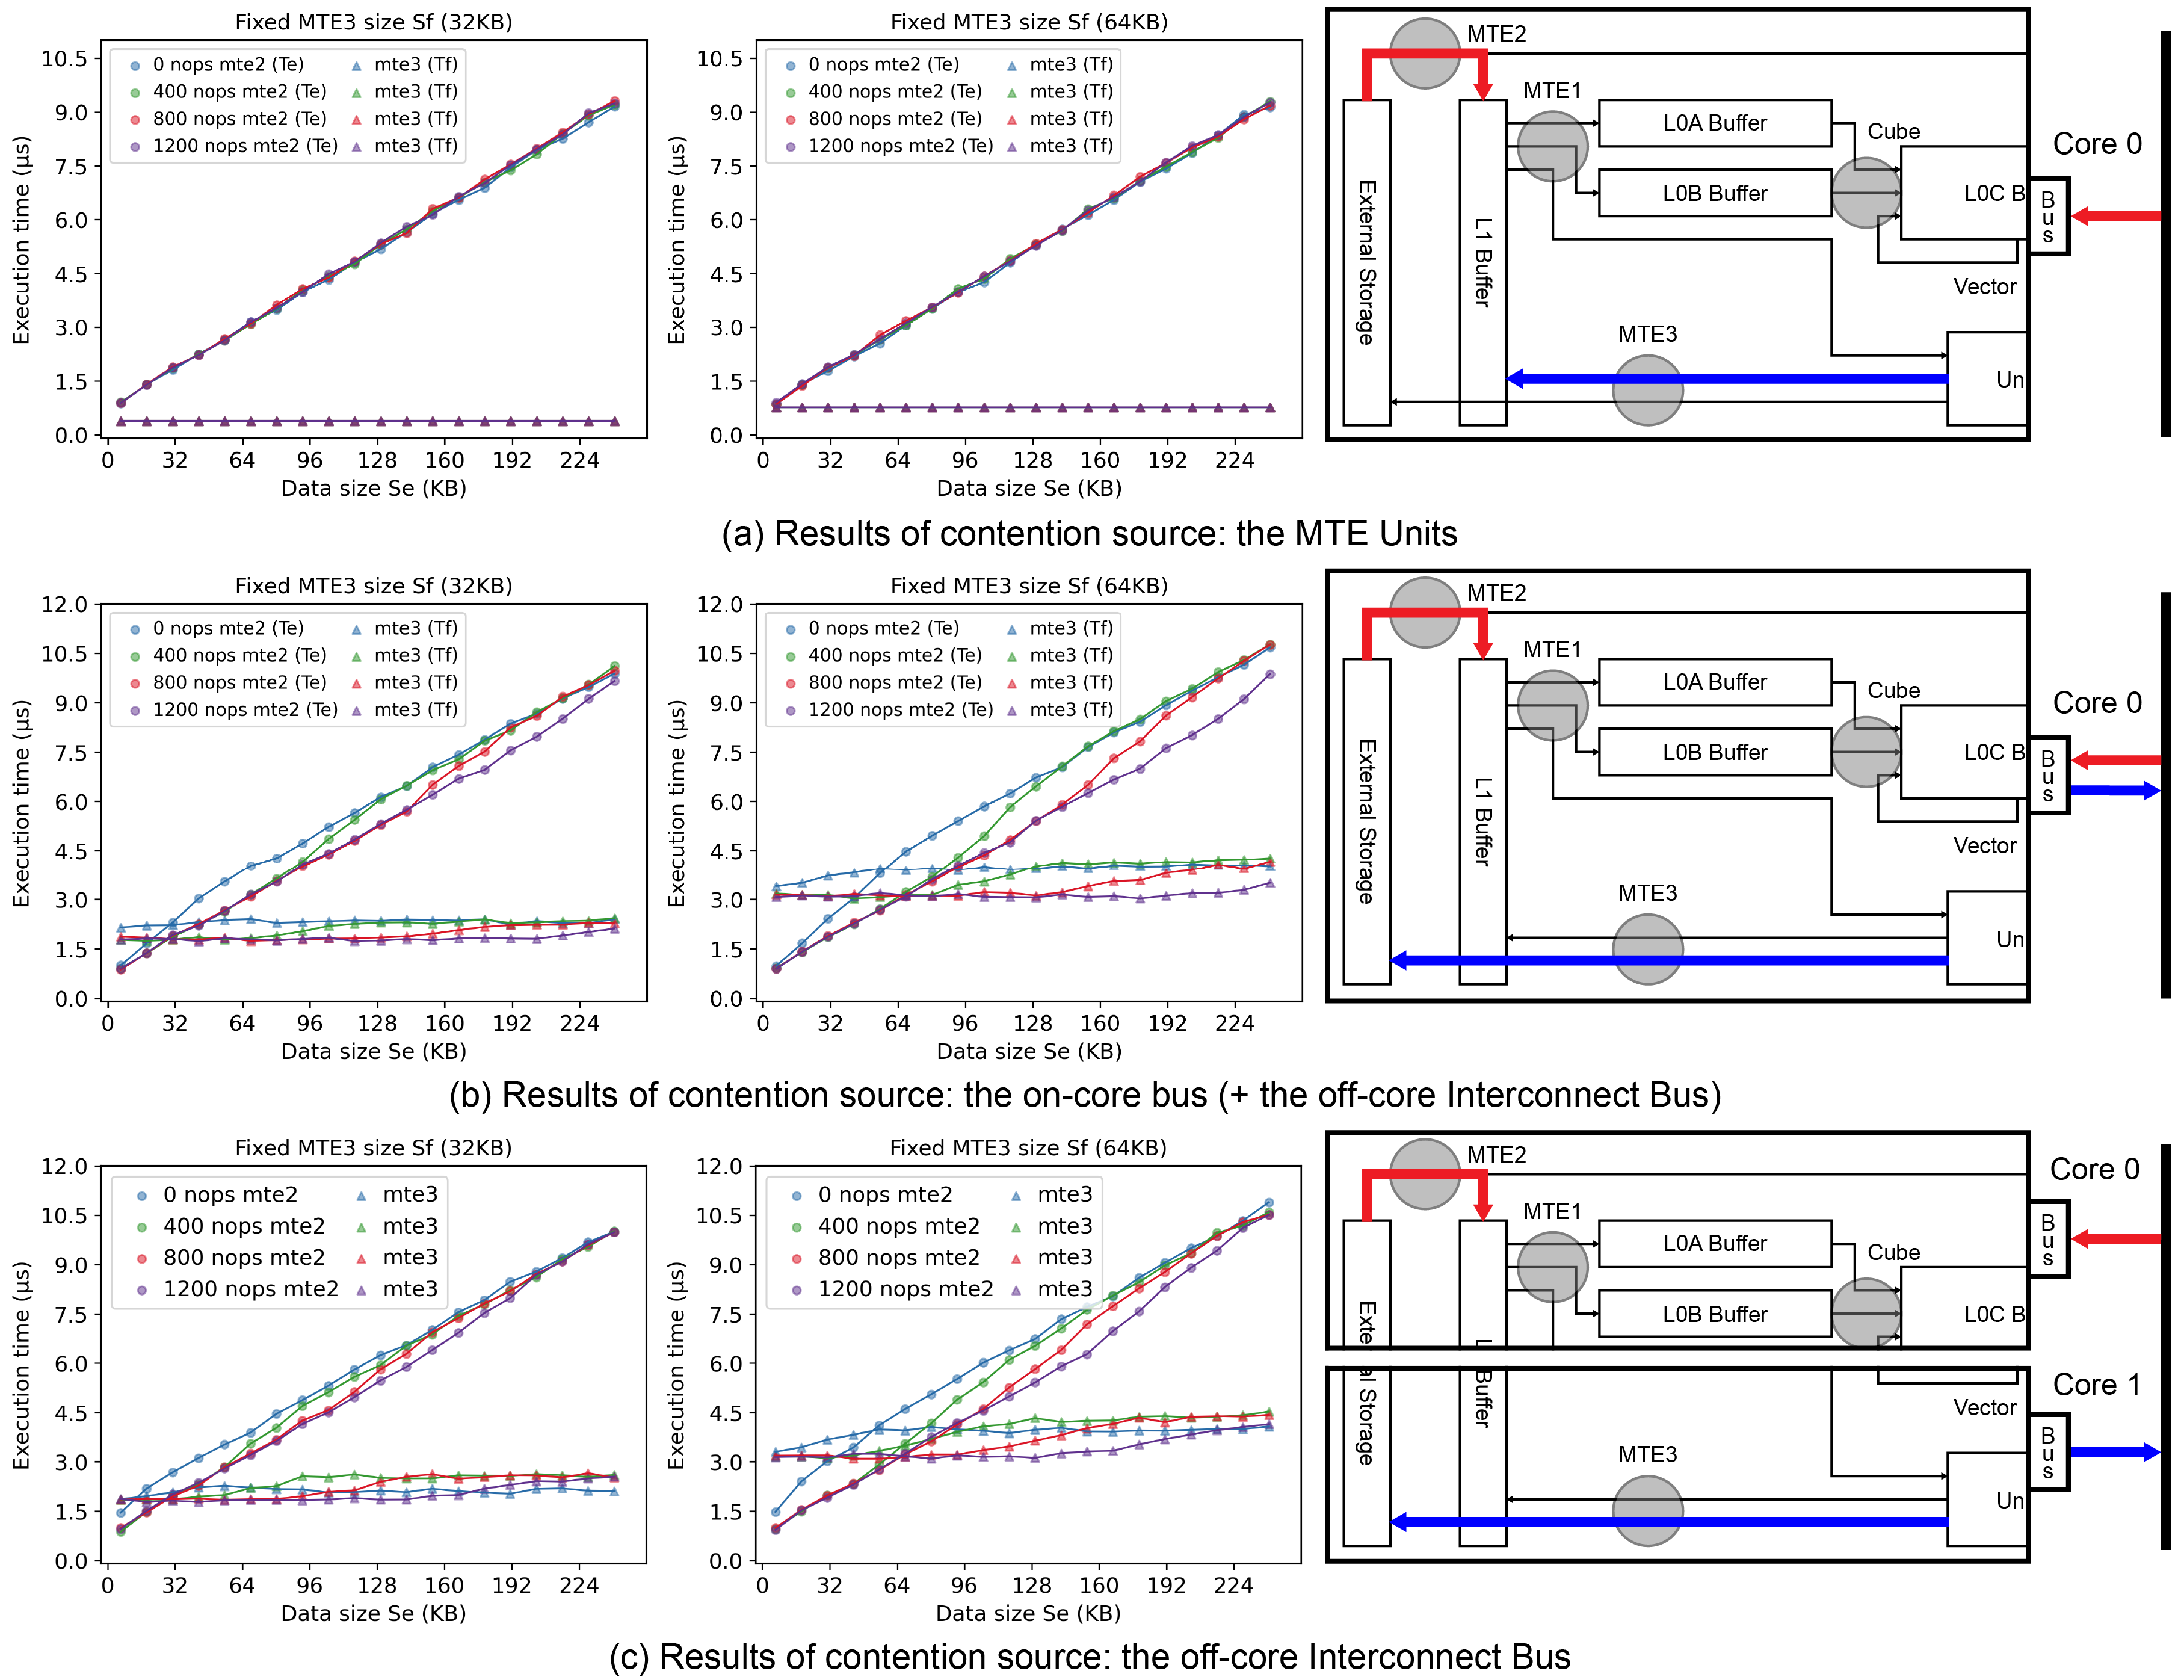
\includegraphics[scale=0.43]{figures/cont_source.png}}
    \caption{Contention source results with the corresponding data paths}
    \label{fig:cont_source}
    \end{figure}

Based on the fundamental benchmark designed in Sec. \ref{sec:ben_des}, we illustrate the benchmark results of the MTE2 and MTE3 Units with the different corresponding data paths in Fig. \ref{fig:cont_source}. We insert NOP instructions as dummy instructions, the number of which (related to $T_s$) are annotated in the legend of figures.

We first call the instructions for transferring data between the external storage and the L1 Buffer (MTE2) and that between the Unified Buffer and L1 Buffer (MTE3) concurrently, which does not involve other data paths. The results in Fig. \ref{fig:cont_source} (a) show that with the variation of $S_f$, $S_e$, and $T_s$, the evaluated execution time $T_f$ and $T_e$ remain unchanged, which indicates no contention happens between the two MTE Units.

By contrast, from the results in Fig. \ref{fig:cont_source} (b) and (c), we observe apparent irregular execution time variations, which present clear bandwidth contention runtime behaviors. For both the MTE2 and MTE3 Units, it is easy to identify the turning points of the three contention statuses we described in Sec. \ref{sec:ben_des}. With the increment of the data size $S_e$, the MTE2 Units report two different slopes in three-segment polylines, where the first segment is before contention, the second is under contention, and the third is after contention. For the MTE3 Units with a fixed data size $S_f$, which were supposed to take a stable execution time, the contentions bring an extra execution time increment and also result in three-segment polylines. The number of the NOP instructions determines $T_s$ and the length of the first segment. The increment of the MTE3 fixed data size $S_f$ extends the second segment, which shows a lower bandwidth because of the sharing of the limited bandwidth under contention. The third segment's slopes are the same as the first for both the MTE2 and MTE3 Units, indicating that the bandwidths recover from the contention without extra side effects.

For the contention source, since it is impracticable to transfer the data without the off-core Interconnect Bus independently, the results shown in Fig. \ref{fig:cont_source} (b) are introduced by both the on-core buses and the off-core Interconnect Bus. Meanwhile, Fig. \ref{fig:cont_source} (c) involves the off-core Interconnect Bus only by placing the two instructions on two DaVinci Cores separately. In this way, in Fig. \ref{fig:cont_source} (c), the on-core bus of Core 0 transfers data to the DaVinci Core with the MTE2 Unit individually and avoid any possibilities for contentions. Comparing the results of Fig. \ref{fig:cont_source} (b) and (c), the execution time, the variation trends, and the slopes are similar, which suggests they activate the same contention source. Therefore, we assert that the contention source of the Ascend 310 processor bus bandwidth is the common part of Fig. \ref{fig:cont_source} (b) and (c), the off-core Interconnect Bus.

\begin{figure}[tbp]
    \centering{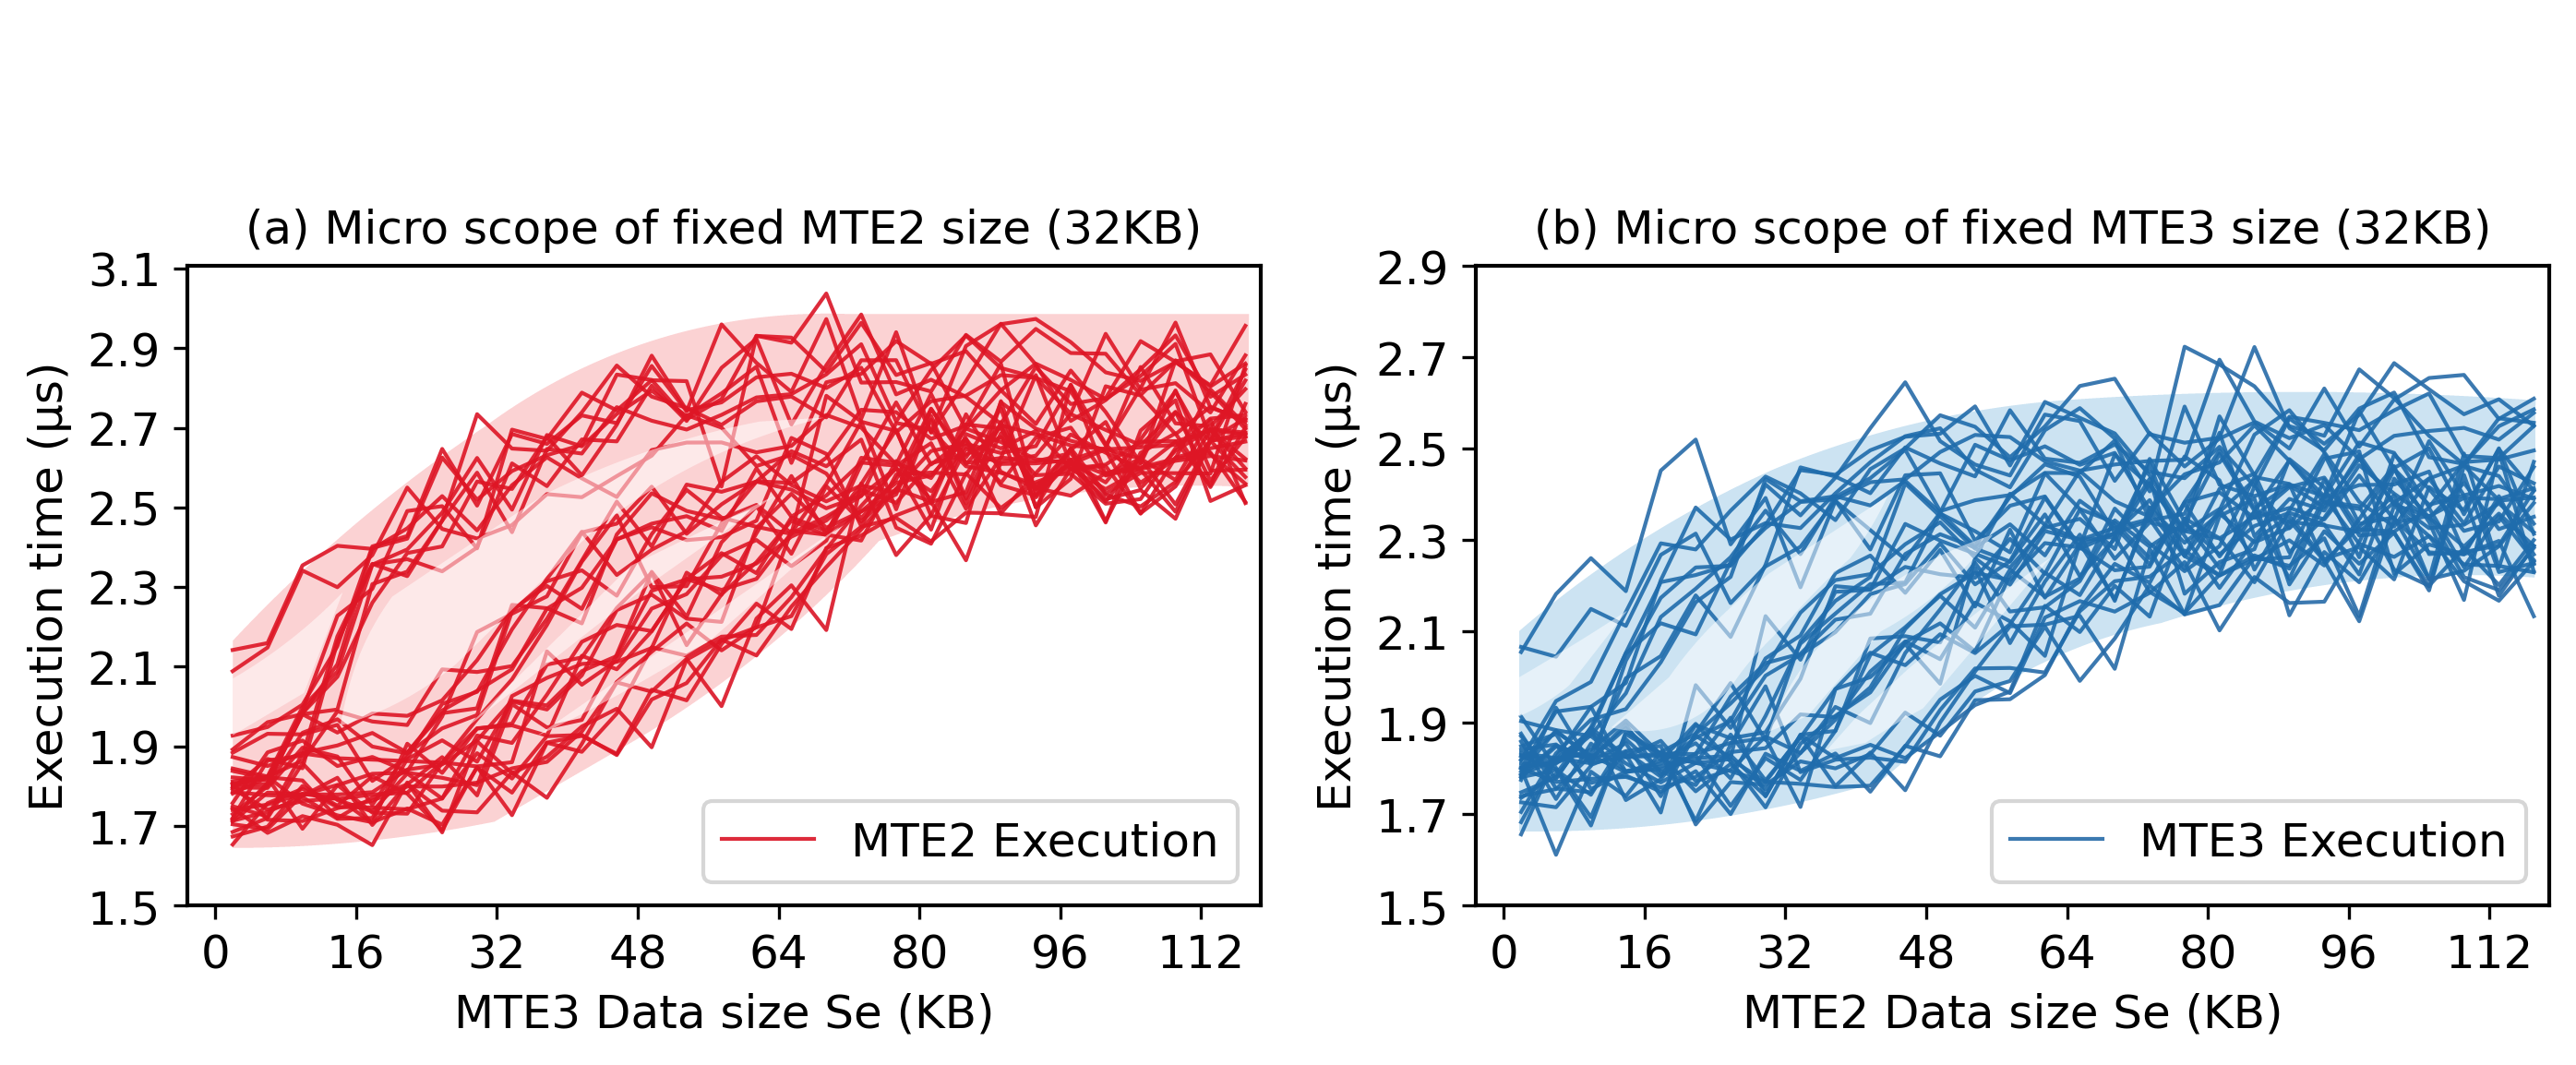
\includegraphics[scale=0.53]{figures/micro_view.png}}
    \caption{The execution of the MTE Units with tiny $T_{s}$ increments}
    \label{fig:micro_view}
    \end{figure}

Fig. \ref{fig:micro_view} shows the results of the second benchmark, where we repeat the benchmark shown in Fig. \ref{fig:cont_source} (b) but increase $T_{s}$ with tiny steps to explore the execution patterns of the MTE Units under contention. Fig. \ref{fig:micro_view} (a) plots the fixed-sized MTE2 Unit execution results ($S_f$ = 32 KB) with the increasing MTE3 Unit data size $S_e$ while Fig. \ref{fig:micro_view} (b) is symmetric. With the increment of $T_{s}$, the beginning of the contention delays, which increases the start points of the second segment we discuss in Sec. \ref{sec:ben_des} accordingly. However, from the results for the two cases, we observe that although $T_{s}$ grows evenly, the start points of the second segments are not averagely distributed along the x-axis but gather at specific points, especially for the MTE3 Unit. The execution patterns show that the MTE Unit does not start the data transfer and forms a contention instantly after execution, suggesting the data is transferred in blocks or segments. We assert that before block transferring, the Interconnect Bus must manage and decide how to share the bandwidth based on the number of executing Units each time.

\subsection{Benchmarks for Bandwidth Sharing under Contention}

After identifying the contention source and runtime behaviors, the maximum contention ratio ($R_{max} = 4$) and the participated hardware units (the MTE2 \& MTE3 Units on two DaVinci Cores) are also determined. We further analyze the detailed policy for the potential participants to share the bandwidth. 

\begin{figure}[tbp]
    \centering{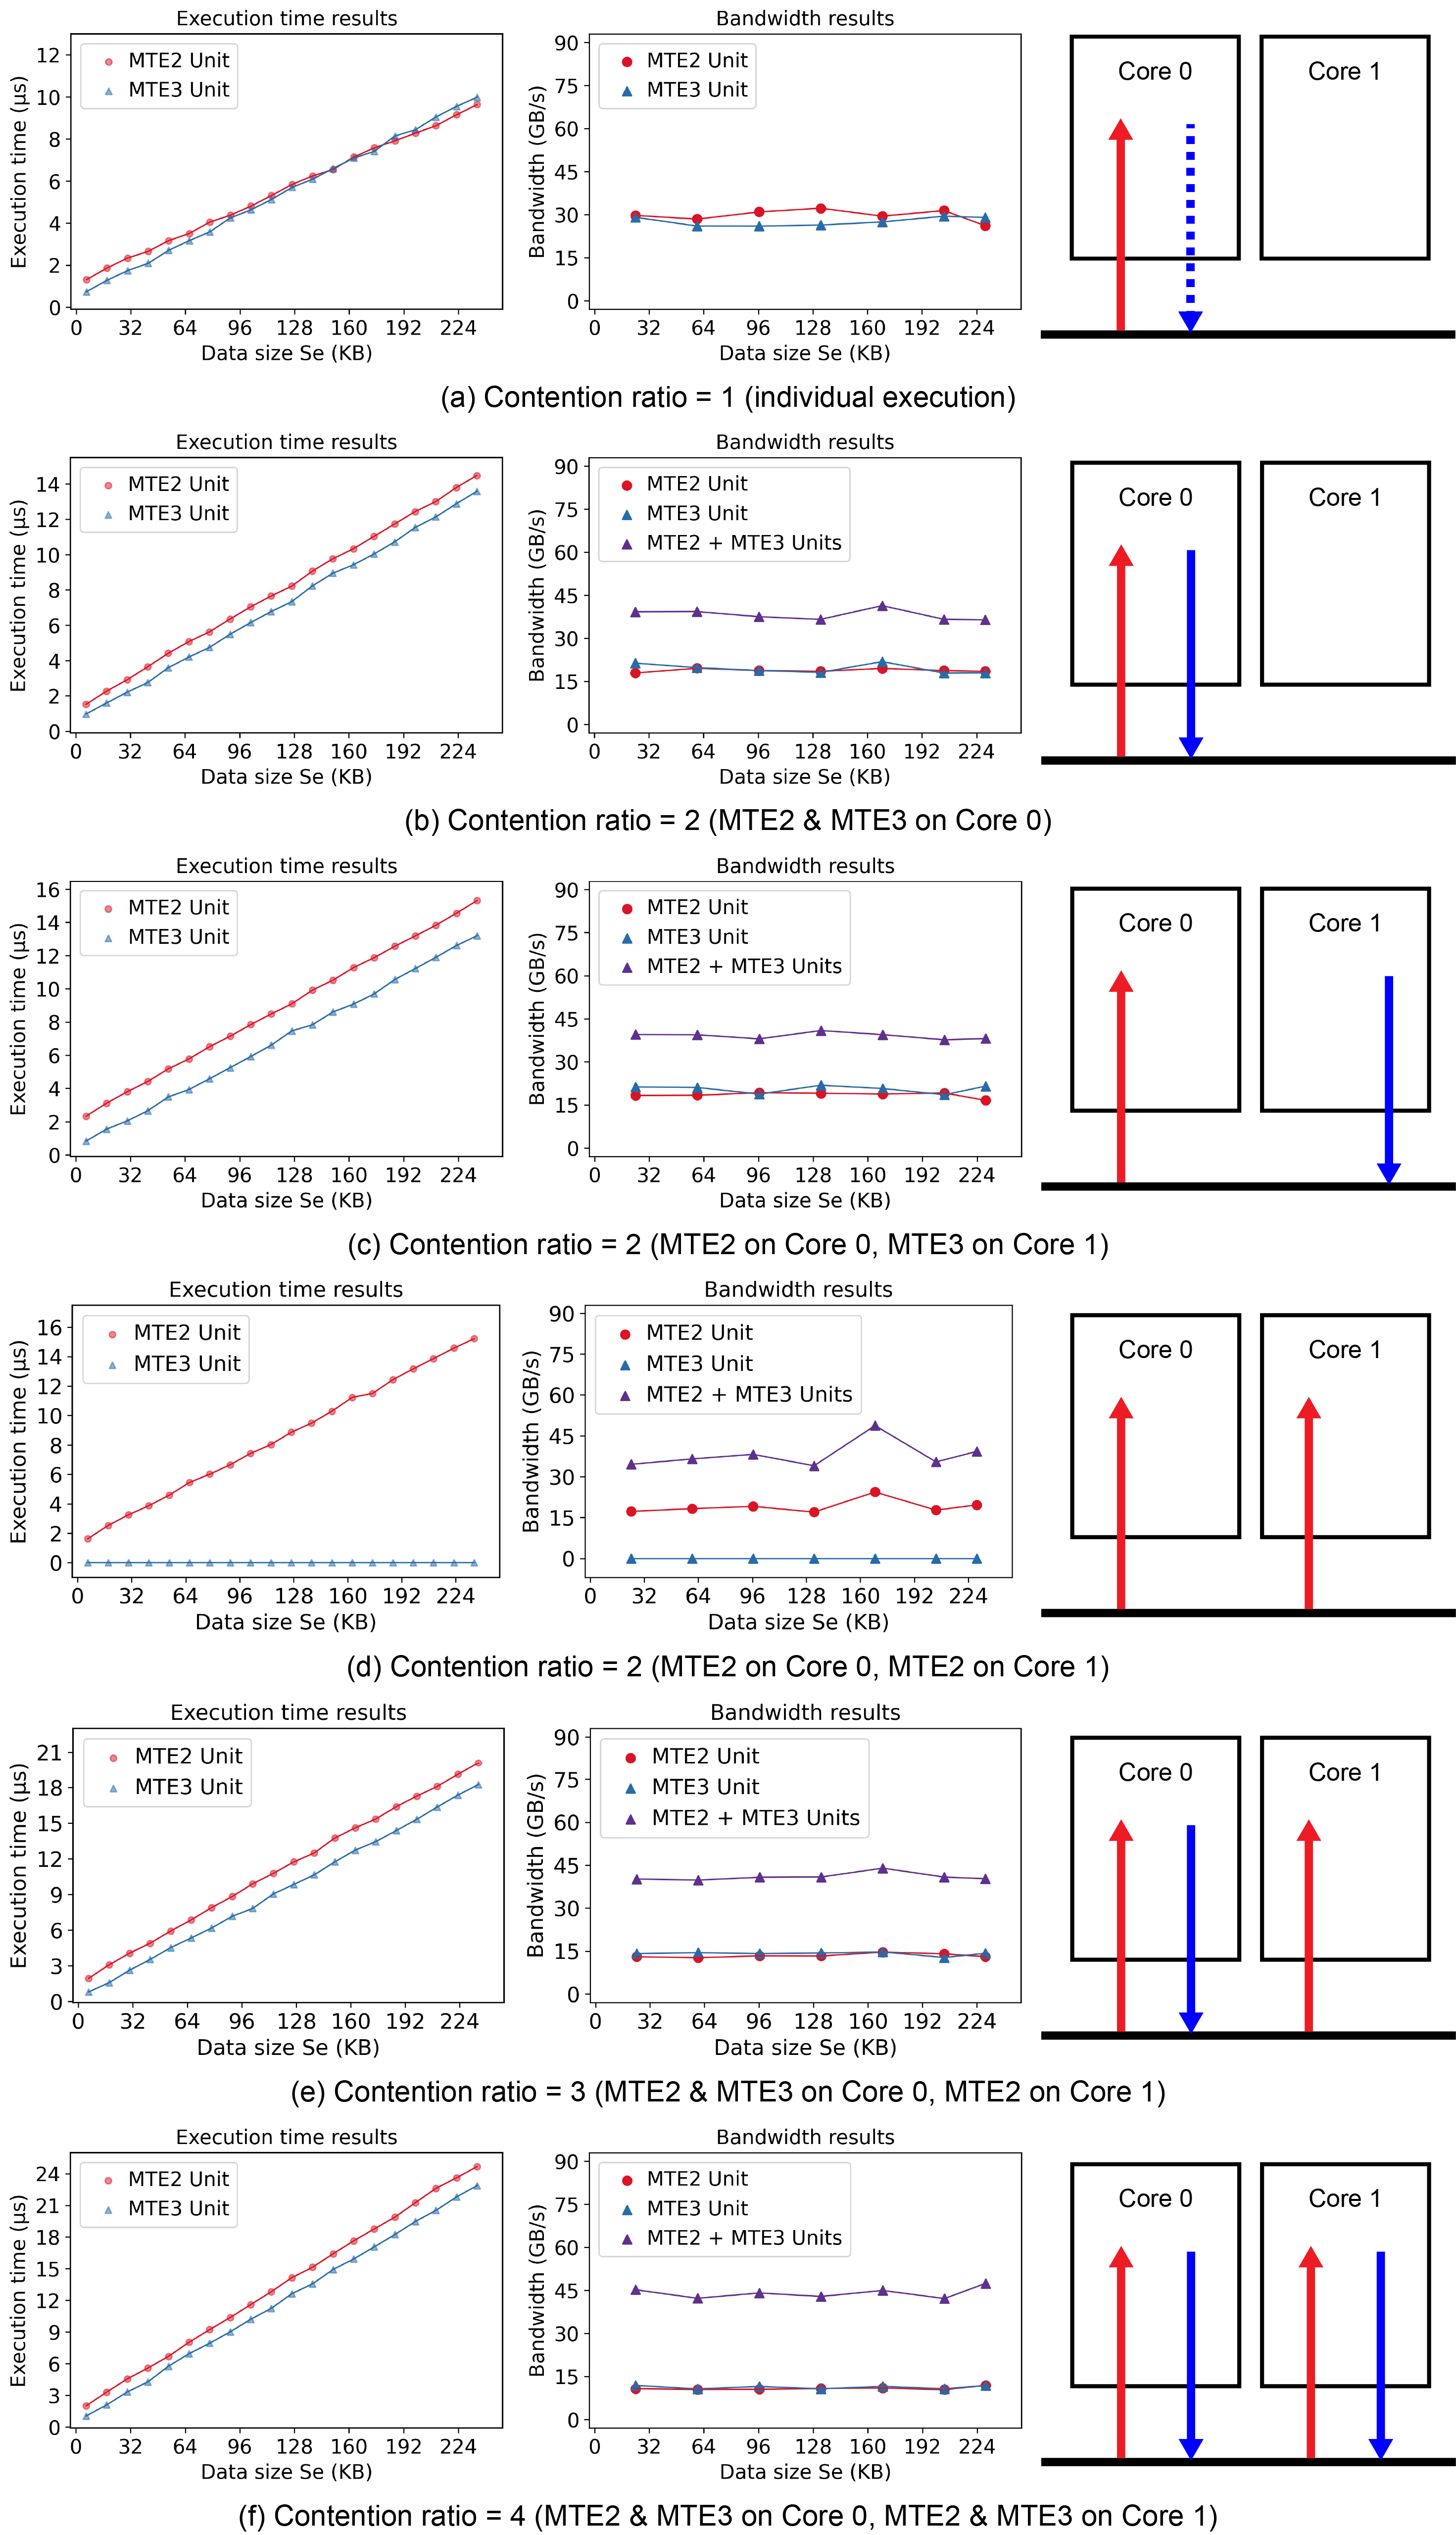
\includegraphics[scale=0.42]{figures/bw_sharing.png}}
    \caption{Bandwidth sharing of the Ascend 310 processors under contention}
    \label{fig:bw_sharing}
    \end{figure}

\subsubsection{Methodology}

We follow the benchmark used in Sec. \ref{sec:cube_bench}, where we increase the processed data sizes and compute the bandwidths under contention using the least-square method. We control the active hardware units, which are involved in the contentions of each case, with different instructions on two DaVinci Cores, respectively. Especially for the MTE3 Units, the benchmarks transfer the data from the Unified Buffer to the external storage, similar to Fig. \ref{fig:cont_source} (b).

\subsubsection{Bandwidth Sharing Results \label{sec:bw_sr_res}}

Fig. \ref{fig:bw_sharing} illustrates the benchmark results for six cases, which include all potential cases under contention. The bandwidth result of each MTE Unit plotted in the chart is the bandwidth of a single operation. Therefore, for the example in Fig. \ref{fig:bw_sharing} (e), the total bandwidth is computed by $2 \times bw_{MTE2} + bw_{MTE3}$. Generally, with the increment of the contention ratio, the total bandwidth (MTE2 $+$ MTE3 Units) also grows with a maximum bandwidth of about 42 GB/s when the contention ratio is 4, shown in Fig. \ref{fig:bw_sharing} (f). 

The bandwidths of writing and reading operations, controlled by the MTE2 and MTE3 Units, are almost equal in all cases while sharing. When the contention ratio is 2, Fig. \ref{fig:bw_sharing} (b, c, d) present three different combinations of the MTE operations, MTE2 and MTE3 operations on Core 0, MTE2 and MTE3 operations on Core 0 and 1, and two MTE2 operations on Core 0 and 1. In contrast to the different units participating, the bandwidth sharing results are the same. Either operation occupies half the total bandwidth in each case, no matter what kind of operation it is or which core the operation is executing. Fig. \ref{fig:bw_sharing} (e) reports the bandwidth results when the contention ratio is 3, where we place two MTE2 operations on two DaVinci Cores with an MTE3 operation on Core 0. The bandwidth of the MTE2 operation is still equal to the MTE3 operation, which implies that the three operations trisect the bandwidth of the Interconnect Bus. Fig. \ref{fig:bw_sharing} (f) also shows a similar averagely sharing result. Therefore, we assert that the Interconnect Bus is a half-duplex bus, where the writing and reading operations can execute concurrently but influence each other. Our later bandwidth contention modeling work is based on the conclusion of the benchmark, where the bandwidth is shared equally by each Unit.

\section{Modeling DaVinci}

After benchmarking the hardware units, this section formally describes the performance model, Verrocchio, especially how it manages the concurrent execution and synchronization.

\subsection{Verrocchio Notation and Parameter Definitions}

We list the notations used in Table \ref{tab:concepts} and part of the hardware parameters used in Table \ref{tab:parameter}. Each instruction of the kernel program $C$ is considered as a discrete event $E_{u, n}$ with an operated data size $Ds_{u, n}$. Since the kernel program is determined, the order of the instructions on each unit is confirmed. Verrocchio uses the pair of $u, n$ to locate instructions. The wall clock updates the death time $T_{u, n}$ of each event.

% Verrocchio Concepts Definitions
\begin{table}[tp]
\caption{Notations used in Verrocchio Performance Model}
\label{tab:concepts}
\begin{center}
\scalebox{0.77}{
    \begin{tabular}{c|c|c}
    \toprule[1pt]
    \textbf{Notations} & \textbf{Description} & \textbf{Value} \\
    \midrule[0.5pt]
    $u$ & The unit number & $0 < u \leq U$  \\
    \midrule[0.5pt]
    $N_{u}$ & The instruction number of the unit $u$ for a kernel program & $0 \leq N_{u}$ \\
    \midrule[0.5pt]
    $n$ & The order number of an instruction on the unit $u$ & $0 < n \leq N_{u}$  \\
    \midrule[0.5pt]
    $E_{u, n}$ & 
        \makecell[c]{A discrete event, an abstraction of the DaVinci instruction, \\ which is the $n$-th event executes on the Unit $u$} & 
        $(u_{a}, u_{b}, r)$ \\
    \midrule[0.5pt]
    $T_{u, n}$ & \makecell[c]{The death time of $E_{u, n}$, \\ which is the wall clock time when $E_{u, n}$ finishes} & $0 \leq T_{u, n}$ \\
    \midrule[0.5pt]
    $P_{u, n}$ & \makecell[c]{The execution period of $E_{u, n}$} & $0 \leq P_{u, n}$ \\
    \midrule[0.5pt]
    $C$ &
        \makecell[c]{The input instructions, an ordered array of a series of $E_{u, n}$} & 
        $\langle E_{u0, n0}, E_{u1, n1},... \rangle$ \\
    \midrule[0.5pt]
    $Ds_{u, n}$ &
        \makecell[c]{The operated data size of $E_{u, n}$} &
        $0 \leq Ds_{u, n}$ \\
    \midrule[0.5pt]
    $S_{E_{u, n}}$ & \makecell[c]{The sorted array to store the subscripts $(u, n)$ \\
        of all Set Flag operations with the same value $(u_{a}, u_{b}, r)$} & $\langle (u0, n0), (u1, n1),... \rangle$ \\
    \midrule[0.5pt]
    $W_{E_{u, n}}$ & \makecell[c]{The sorted array to store the subscripts (u, n) \\
        of all Wait Flag operations with the same value $(u_{a}, u_{b}, r)$} & $\langle (u0, n0), (u1, n1),... \rangle$ \\
        
    \bottomrule[1pt]
    \end{tabular}
}
\end{center}
\end{table}

% Verrocchio Parameters Definitions
\begin{table}[tp]
\caption{Verrocchio hardware parameter definitions of the Ascend 310 processors}
\label{tab:parameter}
\begin{center}

\scalebox{0.78}{
    \begin{tabular}{c|c|c}    
    \toprule[1pt]
    \textbf{Parameters} & \textbf{Description} & \textbf{Value} \\
    \midrule[0.5pt]
    $U$ & The total unit number & 5 \\
    \midrule[0.5pt]
    $r_{max}$ & \makecell[c]{The maximum binary semaphore register number} & 8 \\
    \midrule[0.5pt]
    $Init$ & The initialization time of each instruction & 40 ns \\
    \midrule[0.5pt]
    $T_{kernel}$ & 
        \makecell[c]{The initialization time of \\ DaVinci kernel} & 
        \makecell[c]{2050 ns \\ (inc. 1000 ns for MTE2, \\ 350 ns for MTE3)} \\
    \midrule[0.5pt]
    $Th_{u}$ & \makecell[c]{The throughput (or bandwidth) of the Unit $u$} & Partially Listed in Table \ref{tab:bench}\\

    \bottomrule[1pt]
    \end{tabular}
}
\end{center}
\end{table}

\subsection{Verrocchio Main Performance Modeling Procedure}

We show the Main Performance Modeling Procedure in Alg. \ref{alg:model}. Since the wall clock time when the kernel program finishes is the wall clock time when the last event finishes, which is the largest death time $T_{u, n}$. We assert that the execution time of the kernel program $C$ is the maximum death time of the last Event $E_{u, N_{u}}$ among all Units, as shown in Alg. \ref{alg:model} line 12. 

\begin{algorithm}[tbp]
    \caption{Verrocchio Main Performance Modeling Procedure}
    \label{alg:model}
    
    \SetKwInOut{Input}{input}
    \SetKwInOut{Output}{output}
    
    \Input{
        Kernel program $C = \langle E_{u0, n0}, E_{u1, n1},... \rangle$ \\
        Operated data size $Ds = \langle Ds_{u0, n0}, Ds_{u1, n1},... \rangle$
    }
        
    \Output{
        Kernel wall clock finish time: $T_{end}$
    }
    \BlankLine

    $(T_{u_{0}, n_{0}}, E_{u, n}) \leftarrow (T_{kernel}, E_{u_{0}, n_{0}})$ \\
    \While{$E_{u, n}$ \textbf{is not} the last event in $C$}{
        \Case(\textit{//} normal operations){$E_{u, n} = (0, 0, 0)$}{
            $P_{u,n} \leftarrow Ds_{u,n}\;/\;Th_{u} + Init $  \\
            $T_{u, n} \leftarrow T_{u, n-1} + P_{u, n}$ \\
        }
        \Case(\textit{//} set flag operations){$E_{u, n} > (0, 0, 0)$}{
            $T_{u, n} \leftarrow T_{u, n-1}$
        }
        \Case(\textit{//} wait flag operations){$E_{u, n} < (0, 0, 0)$}{
            $E_{u^{\prime}, n^{\prime}} \leftarrow - E_{u, n}$ \\
            $T_{u, n} \leftarrow T_{u^{\prime}, n^{\prime}} \leftarrow T_{S_{-E_{u, n}}[Index((u, n), W_{E_{u, n}})]}$
        }
        $E_{u, n} \leftarrow$ \textit{the next event in} $C$
    }
    \textbf{Bandwidth\_Contention\_Check}($E_{u, n}$) \\
    $T_{end} \leftarrow \max\limits_{0 < u \leq U}T_{u, N_{u}}$    
\end{algorithm}

For all Events $E_{u, n}$, we divide them into three categories, normal computation or memory operations, Set Flag operations for \verb|set_flag| instructions, and Wait Flag operations for \verb|wait_flag| instructions. The last two categories are the fundamental concepts of the binary semaphore mechanism. Different categories have different procedures to update its death time $T_{u, n}$. We give $E_{u, n}$ a 3-tuple $(u_{a}, u_{b}, r)$ as its value to classify the categories, where $u_{a}, u_{b}$ are the related Units of a Set Flag or Wait Flag operation, $r$ is the corresponding semaphore register, as shown in Fig. \ref{fig:modeling} (a).

\subsubsection{Normal Computation Or Memory Operations}

\begin{figure}[tbp]
    \centering{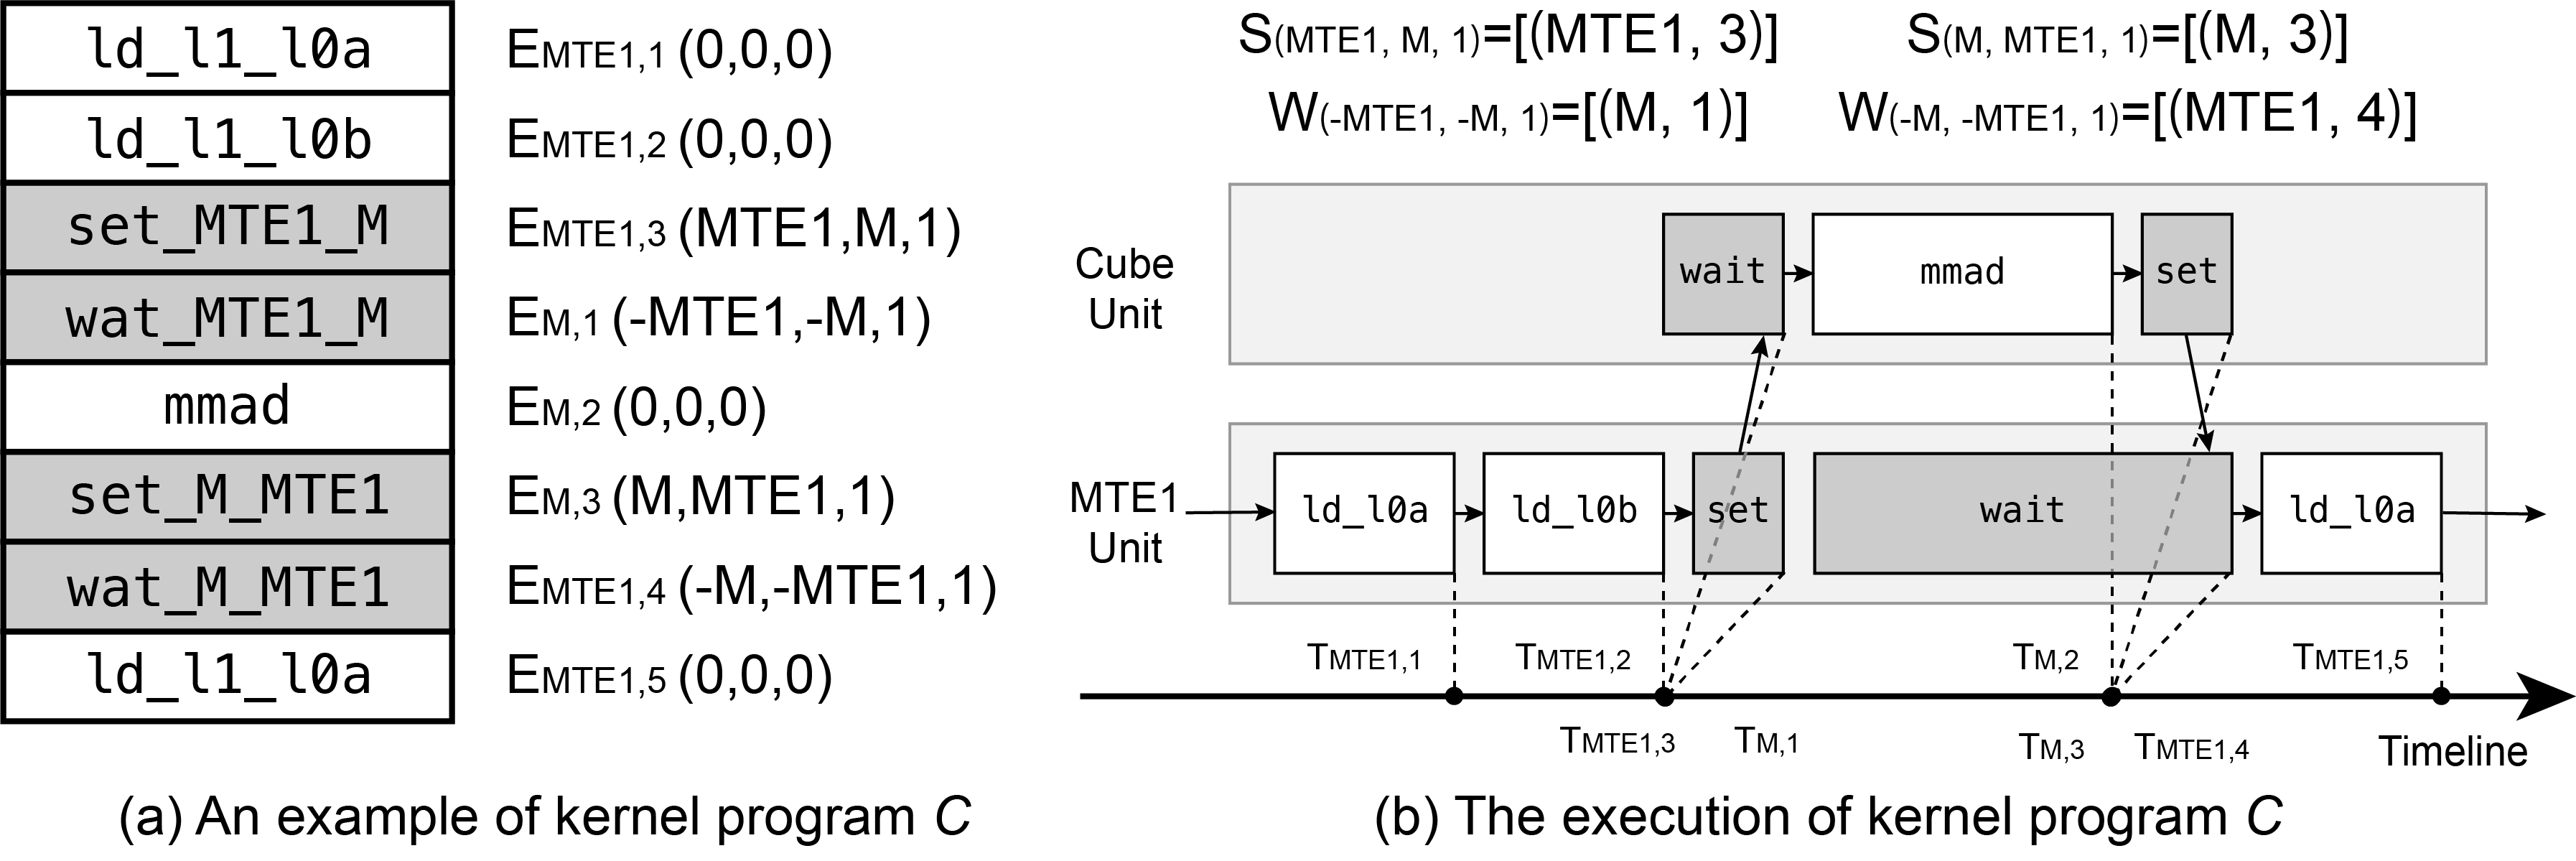
\includegraphics[scale=0.39]{figures/modeling.png}}
    \caption{An example of Verrocchio main performance modeling procedure}
    \label{fig:modeling}
\end{figure}

For the normal operations, we set $E_{u, n} = (0, 0, 0)$, which means $E_{u, n}$ is not related to the binary semaphore mechanism. For each normal computation or memory operation $E_{u, n}$, we first compute the corresponding static execution period $P_{u, n}$ to quantify how long the $E_{u, n}$ could occupy the Unit $u$. In general,  $P_{u, n}$ is computed as shown in Alg. \ref{alg:model} line 4. According to the FIFO policy, the incidence of $E_{u, n}$ should be immediately after the death of $E_{u, n-1}$. Hence, we compute the death $T_{u, n}$ of $E_{u, n}$ as the sum of the last death time $T_{u, n-1}$ on the same Unit $u$ and the event execution period $P_{u, n}$, as shown in Alg. \ref{alg:model} line 5.

\subsubsection{Set Flag Operations}

For the Set Flag operations, we set $E_{u, n} > (0, 0, 0)$. For the example in Fig. \ref{fig:modeling} (a), the instruction \verb|set_MTE1_M| is converted to $E_{MTE1, 3} = (MTE1, M, 1)$, which means the MTE1 Unit has finished its work, and the Cube Unit should terminate its corresponding Wait Flag operation and continue its next operation with Register 1. Since the Set Flag operations do not suspend or finish any workloads, the death time $T_{u, n}$ equals the last death time $T_{u, n-1}$.

Before the Main Performance Modeling Procedure, we create and maintain an array $S_{E_{u, n}}$ to store the Set Flag operations with the subscript of the 3-tuple $(u_{a}, u_{b}, r)$. We store the 2-tuple $(u, n)$ of $E_{u, n}$, the identification of the Set Flag operation. We have the definition of $S_{E_{u, n}}$ shown below:

\begin{equation}
\begin{aligned}
S_{E_{u_{1}, n_{1}}} = & S_{E_{u_{2}, n_{2}}} = S_{(u_{a}, u_{b}, r)} = \langle (u_{1}, n_{1}), (u_{2}, n_{2}), ... \rangle \\
& \forall E_{u, n} > (0, 0, 0), n_{i} < n_{j}, \forall i < j
\end{aligned}
\end{equation}

where the array $S_{E_{u, n}}$ is sorted according to the operation order number $n$.

\subsubsection{Wait Flag Operations}

For the Wait Flag operations, we set $E_{u, n} < (0, 0, 0)$, which is symmetric to the Set Flag operation definition. For the example in Fig. \ref{fig:modeling} (a), the instruction \verb|wait_MTE1_M| is converted to $E_{M, 1} = (-MTE1, -M, -1)$. We also create and maintain an array $W_{E_{u, n}}$ to store the 2-tuple $(u, n)$, as shown below:

\begin{equation}
\begin{aligned}
W_{E_{u_{1}, n_{1}}} = W_{E_{u_{2}, n_{2}}} = & W_{(-u_{a}, -u_{b}, -r)} = \langle (u_{1}, n_{1}), (u_{2}, n_{2}), ... \rangle \\
\forall E_{u, n} < & (0, 0, 0), n_{i} < n_{j}, \forall i < j
\end{aligned}
\end{equation}

For a Wait Flag operation $E_{u, n}$, its corresponding Set Flag operation $E_{u^{\prime}, n^{\prime}}$ must exist, where $E_{u, n} = - E_{u^{\prime}, n^{\prime}}$, as shown in Alg. \ref{alg:model} line 9. The array $S$ and $W$ are used to locate the related Set Flag and Wait Flag operation pair. Since DaVinci Cores have no memory heap or stack structure but only registers to store the semaphores, the Wait Flag operation order number in $W_{E_{u, n}}$ equals the order number of its corresponding Set Flag operation in $S_{E_{u^{\prime}, n^{\prime}}}$. We introduce a function $Index(x, Array)$ to return the position of $x$ in an array $Array$ without duplicated elements, then we have the relation:

\begin{equation}
Index((u, n), W_{E_{u, n}}) = 
    Index((u^{\prime}, n^{\prime}), S_{E_{u^{\prime}, n^{\prime}}}) = 
    Index((u^{\prime}, n^{\prime}), S_{- E_{u, n}})
\end{equation}

Hence, we have:

\begin{equation}
(u^{\prime}, n^{\prime}) = S_{- E_{u, n}}[Index((u, n), W_{E_{u, n}})]
\end{equation}

Since a Wait Flag operation blocks the Unit until the corresponding Set Flag operation is done, the death time of the Wait Flag operation equals the Set Flag operation death time. For the example in Fig. \ref{fig:modeling} (b), we compute $T_{M, 1}$ as follows:

\begin{equation}
\label{eq:wait}
T_{M, 1} = T_{S_{-E_{M, 1}}[Index((M, 1), W_{E_{M, 1}})]}
    = T_{S_{(MTE1, M, 1)}[0]}
    = T_{MTE1, 3}
\end{equation}

\subsubsection{Bandwidth Contention Updating}

As we discussed, the bandwidth contention of the Interconnect Bus influences the performance of the MTE2 and MTE3 Units significantly. The runtime behaviors we expose in Sec. \ref{sec:runtime} show that each time the two Units start to run concurrently, the contention occurs, and the related bandwidth changes; when either of the Units finishes, the contention ends, and the Units regain the original bandwidth. For the example in Fig. \ref{fig:contention} (a), at $T_{MTE3, 1}$, when the MTE3 starts to execute the instruction \verb|ld_ub_to_gm|, the contention begins; when the MTE2 Unit finishes its work at $T_{MTE2, 1}$, the contention is finished. Therefore, the contention status changes at the event death time. Verrocchio checks whether a contention appears or disappears when an event is finished to update the death time of the related events.

\begin{figure}[tbp]
    \centering{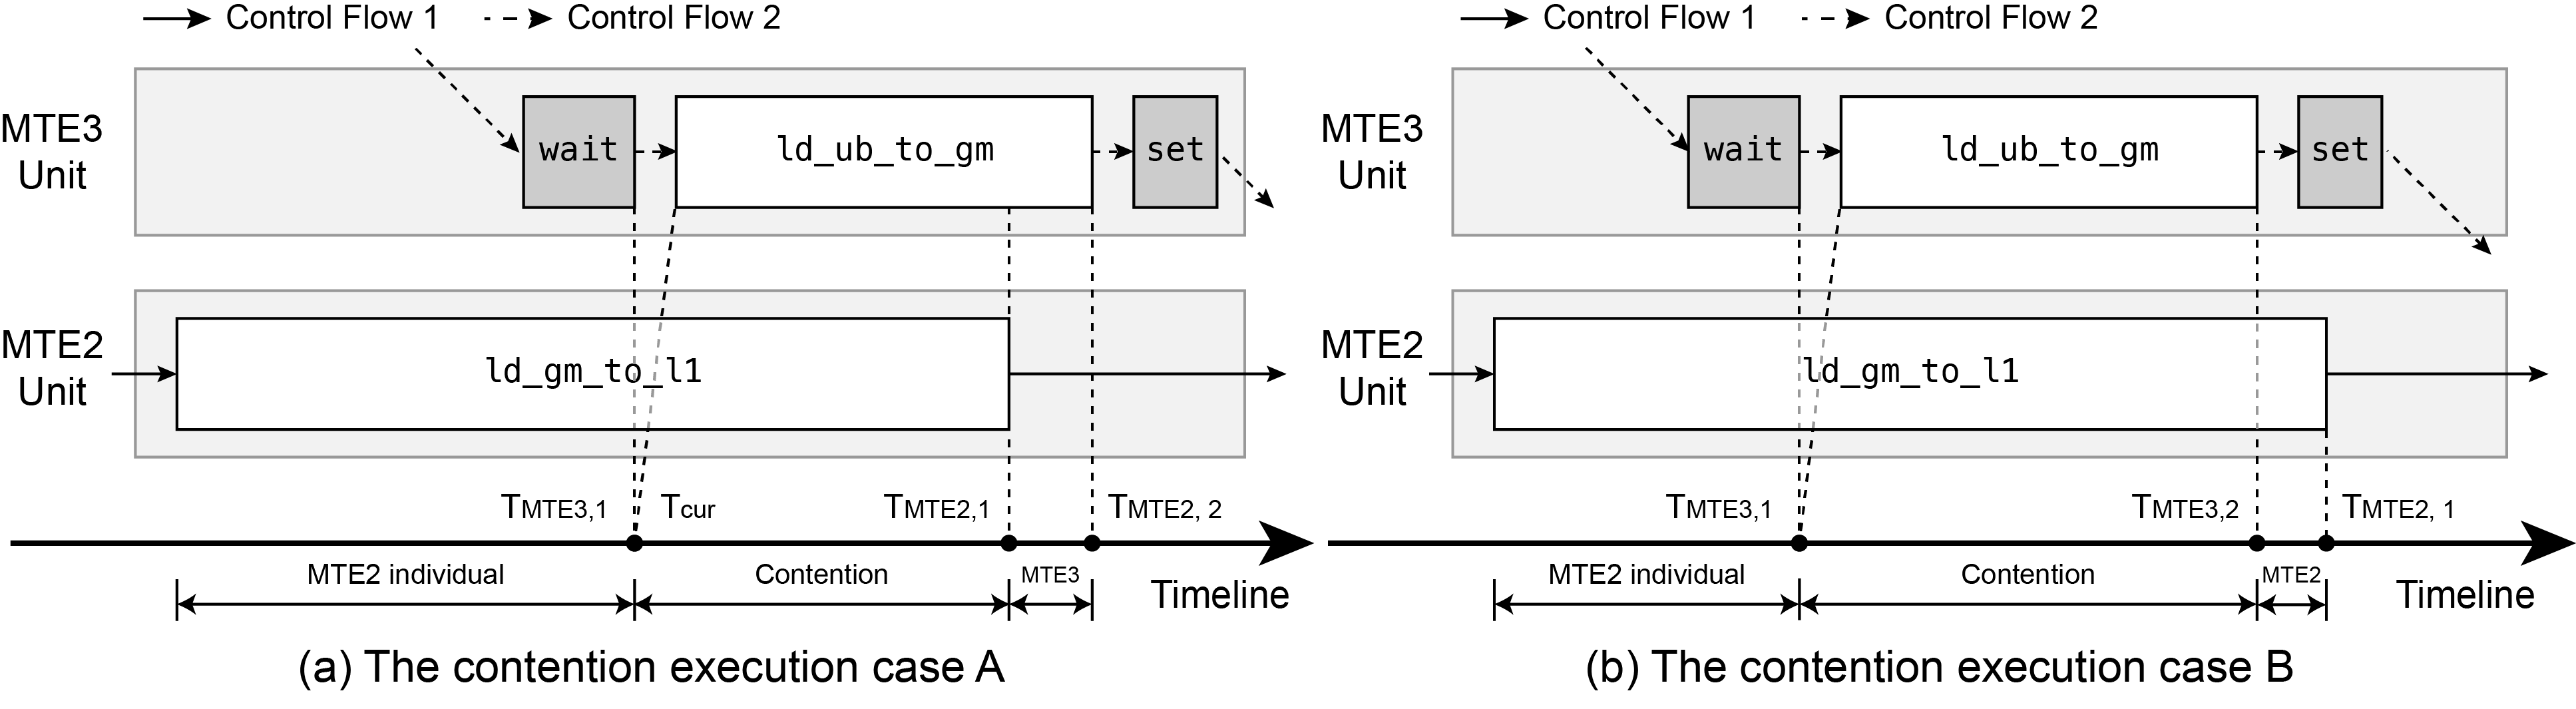
\includegraphics[scale=0.37]{figures/contention.png}}
    \caption{Examples of Verrocchio contention execution}
    \label{fig:contention}
\end{figure}

We first compute the left data size of the event, which is influenced by the contention status change. For an event $E_{u, n}$, we compute the left data size as shown below:

\begin{equation}
Ds^{\prime}_{u, n} = Ds_{u, n} \times \frac{T_{u, n} - T_{cur}}{P_{u, n}}
\end{equation}

where $T_{cur}$ is the current global time, also the death time of the latest event triggering the bandwidth contention, e.g., $T_{MTE3, 1} = T_{cur}$ in Fig. \ref{fig:contention} (a), $Ds^{\prime}_{u, n}$ is the data size left for the new contention status. Then we update the event death time as follows:

\begin{equation}
T^{\prime}_{u, n} = T_{cur} + Ds^{\prime}_{u,n}\;/\;Th^{\prime}_{u}
\end{equation}

where $Th^{\prime}_{u}$ is the bandwidth of the Unit $u$ at the new contention status, $T^{\prime}_{u, n}$ is the new death time. For $Th^{\prime}_{u}$, we strictly follow our conclusions in Sec. \ref{sec:bw_sr_res}, where multiple Units equally share the bandwidth. The potential executions with a contention are divided into two cases shown in Fig. \ref{fig:contention}, based on the relationship of the two events' execution period. For the case in Fig. \ref{fig:contention} (a), both units suffer one contention status change; for Fig. \ref{fig:contention} (b), one unit suffers two contention status changes, experiencing the three-segment polyline of bandwidths discussed in Sec. \ref{sec:runtime}. 

\subsection{Multi-core Execution Performance Modeling \label{sec:multi-core}}

According to our benchmark results, the DaVinci hardware units can be classified into two categories, the one which relies on the independent on-core resources and the other which occupies the Interconnect Bus and causes contentions. For the first category, the throughput $Th_{single}$ of every single core does not change (as a const value $C_{single}$) in the multi-core execution, and the total unit throughput $Th_{total}$ of all cores increases proportionally.

\begin{equation}
\label{eq:first}
Th_{single} = C_{single} \qquad Th_{total} = N \times Th_{single}
\end{equation}

where $N$ is the number of the activated DaVinci Cores. For the second category, as our benchmarks report in Sec. \ref{sec:bw_sr_res}, the throughputs of all single core $Th_{single}$ averagely share the total throughput.

\begin{equation}
\label{eq:second}
Th_{single} = \frac{Th_{total}}{N} \qquad Th_{total} = C_{total} 
\end{equation}

Like most multi-core accelerators, we assume that multi-core DaVinci processors continue to adopt the SIMD execution model, which means the programs are tiled and distributed to multiple cores. We focus on a general normal computation or memory operation $E_{u, n}$, submitted to multiple DaVinci Cores, as shown in Fig. \ref{fig:multi-core}, where each bar is a tile of $E_{u, n}$, e.g. $Tile_{1}$, $Tile_{2}$. To model the differences in the $E_{u, n}$ incident time $T_{u, n_{inc}}$ in all DaVinci Cores (e.g. $T_{inc_{2}} - T_{inc_{1}}$), we introduce $\delta_{t}$, which can be measured in our benchmarks. It represents the average interval between the two nearest incident times among all DaVince Cores.

For each tile of $E_{u, n}$ among all DaVinci Cores, the workloads (data sizes) $Ds_{single}$ are the same. Because of $\delta_{t}$, the tile of $E_{u, n}$ on each core shows a stepped execution pattern with a start-up time. The execution period $P_{u, n}$ of $E_{u, n}$ for case (a) in Fig. \ref{fig:multi-core} is calculated as below:

\begin{figure}[tbp]
    \centering{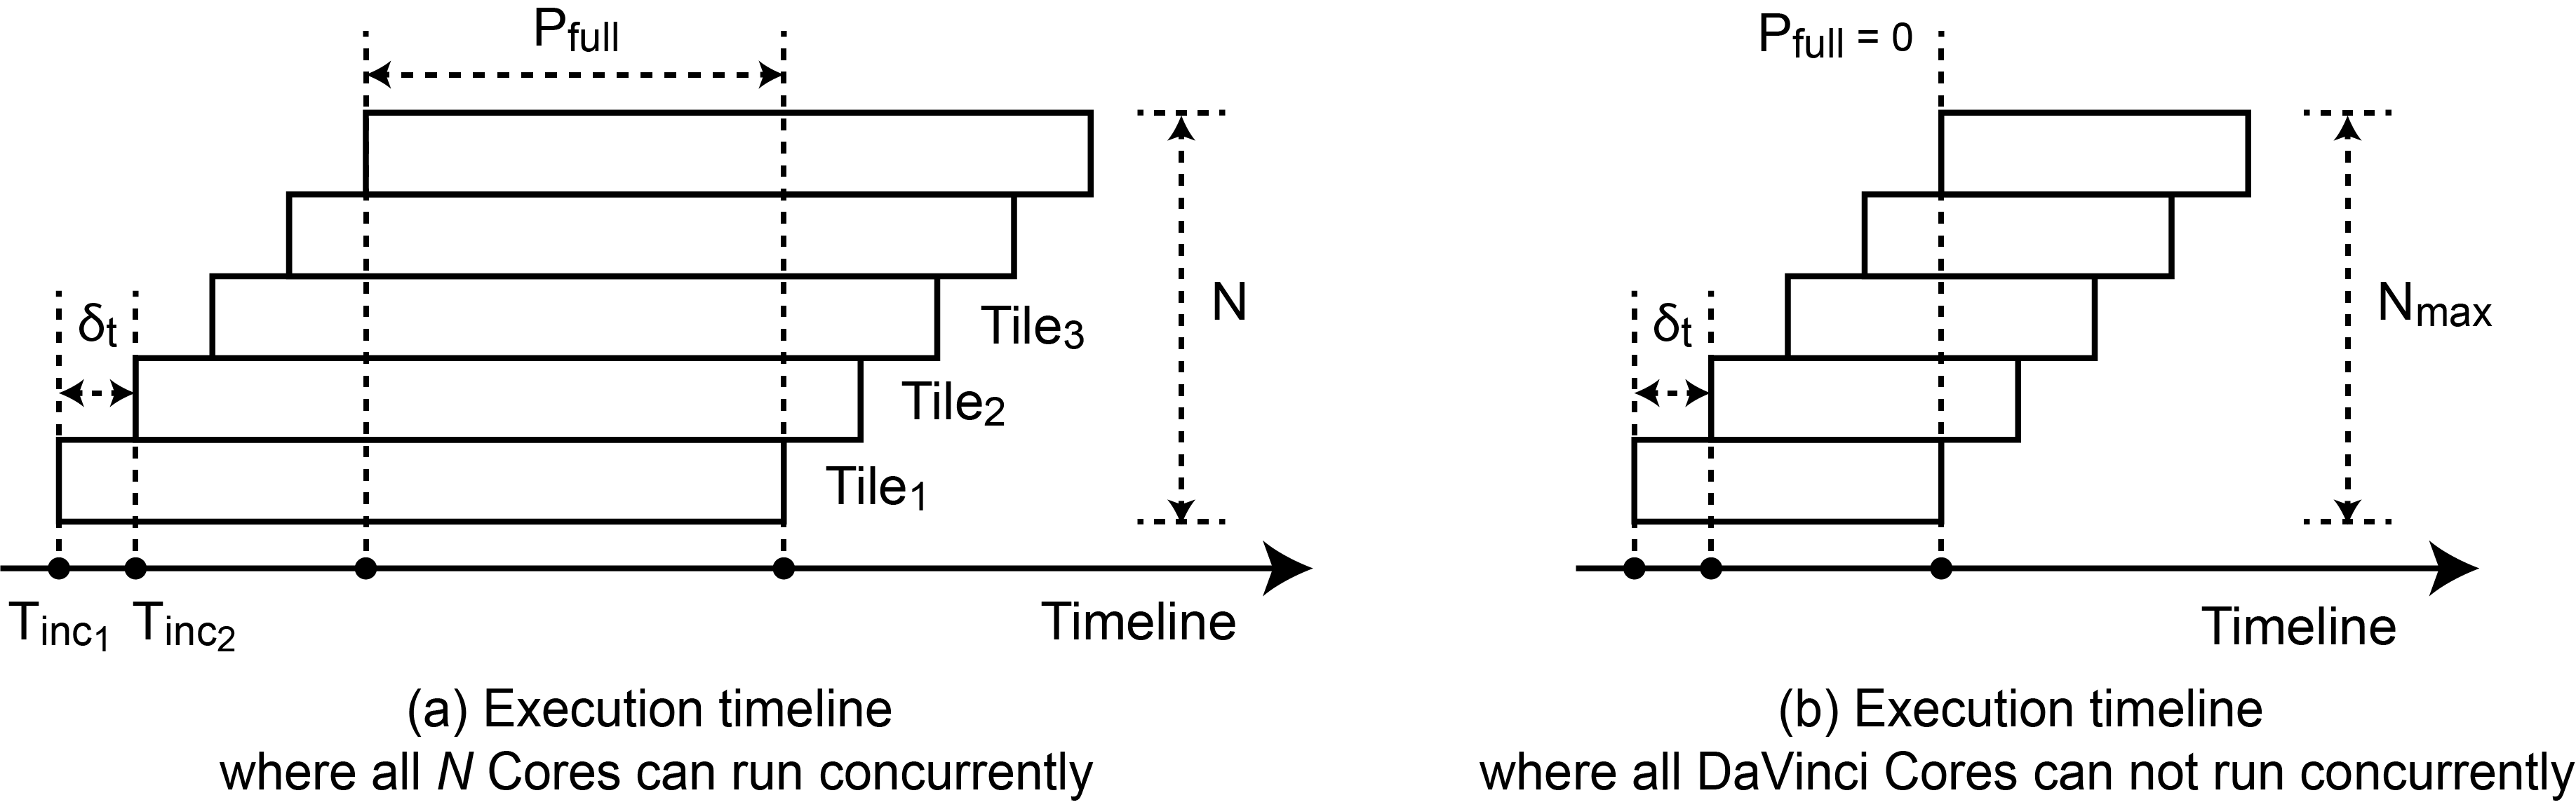
\includegraphics[scale=0.38]{figures/multicore.png}}
    \caption{
    Execution timeline of $E_{u, n}$, which is tiled and submitted to multiple DaVinci Cores}
    \label{fig:multi-core}
    \end{figure}    

\begin{equation}
P_{u, n} = 2 (N - 1) \delta_{t} + P_{full}
\end{equation}

where $P_{full}$ is the period when all the cores are running concurrently. The execution period $P_{u, n}$ of $E_{u, n}$ for case (b) is calculated as below:

\begin{equation}
P_{u, n} = 2 (N_{max} - 1) \delta_{t}
\end{equation}

where $N_{max}$ is the maximized all-busy core number for the event $E_{u, n}$. Then, to calculate $P_{u, n}$, we must determine $P_{full}$ and $N_{max}$ first. For the first category of the units, which relies on the independent on-core resources only, we have Eq. \ref{eq:first_eq} for the case (a) in Fig. \ref{fig:multi-core}:

\begin{equation}
\label{eq:first_eq}
\begin{aligned}
    2 Th_{single} \delta_{t} \times \sum_{i=1}^{N-1}{i} + & N \times Th_{single} P_{full} = N \times Ds_{single} \\
    \implies P_{full} = & \frac{Ds_{single} - (N - 1) Th_{single} \delta_{t}}{Th_{single}} 
\end{aligned}
\end{equation}

Fig. \ref{fig:multi-core} shows that, the condition converting the case (a) to the case (b) is $P_{full} = 0$, which means that all DaVinci Cores cannot run concurrently and then the core number $N$ is $N_{max}$. Then we have the relation shown below:

\begin{equation}
P_{full} = \frac{Ds_{single} - (N_{max} - 1) Th_{single} \delta_{t}}{Th_{single}} = 0 \implies
N_{max} = \frac{Ds_{single}}{Th_{single} \delta_{t}} + 1
\end{equation}

We follow a similar idea for the second category of units as for the first category units. Hence, we list the equation below:

\begin{equation}
\label{eq:second_eq}
    \begin{aligned}
    2 Th_{total} \delta_{t} \times (N - 1) + Th_{total} P_{full} & = N \times Ds_{single} \\
    P_{full} = \frac{N Ds_{single} - 2 (N - 1) Th_{total} \delta_{t}}{Th_{total}}
    \  
    N_{max} & = \frac{2 Th_{total} \delta_{t}}{2 Th_{total} \delta_{t} - Ds_{single}}
    \end{aligned}
\end{equation}

The Ascend 310 processors are the simplest DaVinci architecture processors and have two DaVinci Cores, and then we have $N = 2$. According to our benchmark results, as shown in Table \ref{tab:bench}, $\delta_{t} \approx 61 ns$, which is $2.5\%$ of the kernel launch time and can be ignored. Hence, in the double-core execution, the total time can be simplified to $P_{u, n} = P_{full} = Ds_{single} / Th_{single}$ for the first category of units or $P_{u, n} = N \times Ds_{single} / Th_{total}$ for the second category.

% Evaluation Section

\section{Evaluation}

This section evaluates the accuracy of Verrocchio. We first implement several basic kernels for the accuracy evaluations. Then as a complicated test case and a demonstration of the usage of Verrocchio, we show a matrix multiplication optimizing process guided by Verrocchio. All the experiment results are collected by Huawei's official profiler on the Ascend 310 processor (two DaVinci Cores) with Huawei Kunpeng 920 2.6GHz CPU equipped.

\subsection{Sample Kernel Evaluation}

Table \ref{tab:kernel_type} lists the sample kernels we implement for evaluations. The cases include memory transfers, single computations, and several basic applications. We evaluate the accuracy results for both single-core and double-core situations. Fig. \ref{fig:tiny} illustrates the evaluated error rate results for each case.

Generally, Verrocchio reports high accuracy results. For the single-core execution, the average error rate is $2.62\%$; for the double-core execution, the result is $2.30\%$. The error rates among all cases do not show a system error but are randomly scattered around the baseline. The single-core kernel \textit{mte1B} reports the maximum error rate of $7.33\%$. On the other hand, for the double-core execution, \textit{mte1B} reports a much lower error rate of $3.14\%$. Since the MTE1 Unit is the independent on-core unit we discussed in Sec. \ref{sec:multi-core}, which does not suffer the performance loss in the multi-core execution, \textit{mte1B} is expected to show similar error rates in the two situations. Therefore, the practical results suggest that the MTE1 Unit is not stable as other independent on-core units, which may require deeper analyses. In addition, we observe that the error rates of the Application kernels and the Memory Transfer kernels are higher than the Single Operation kernels, which indicates that the memory transfers, especially between the on-core buffers and the external storage, are the main prediction error sources of Verrocchio.

\begin{figure}[tbp]
    \centering{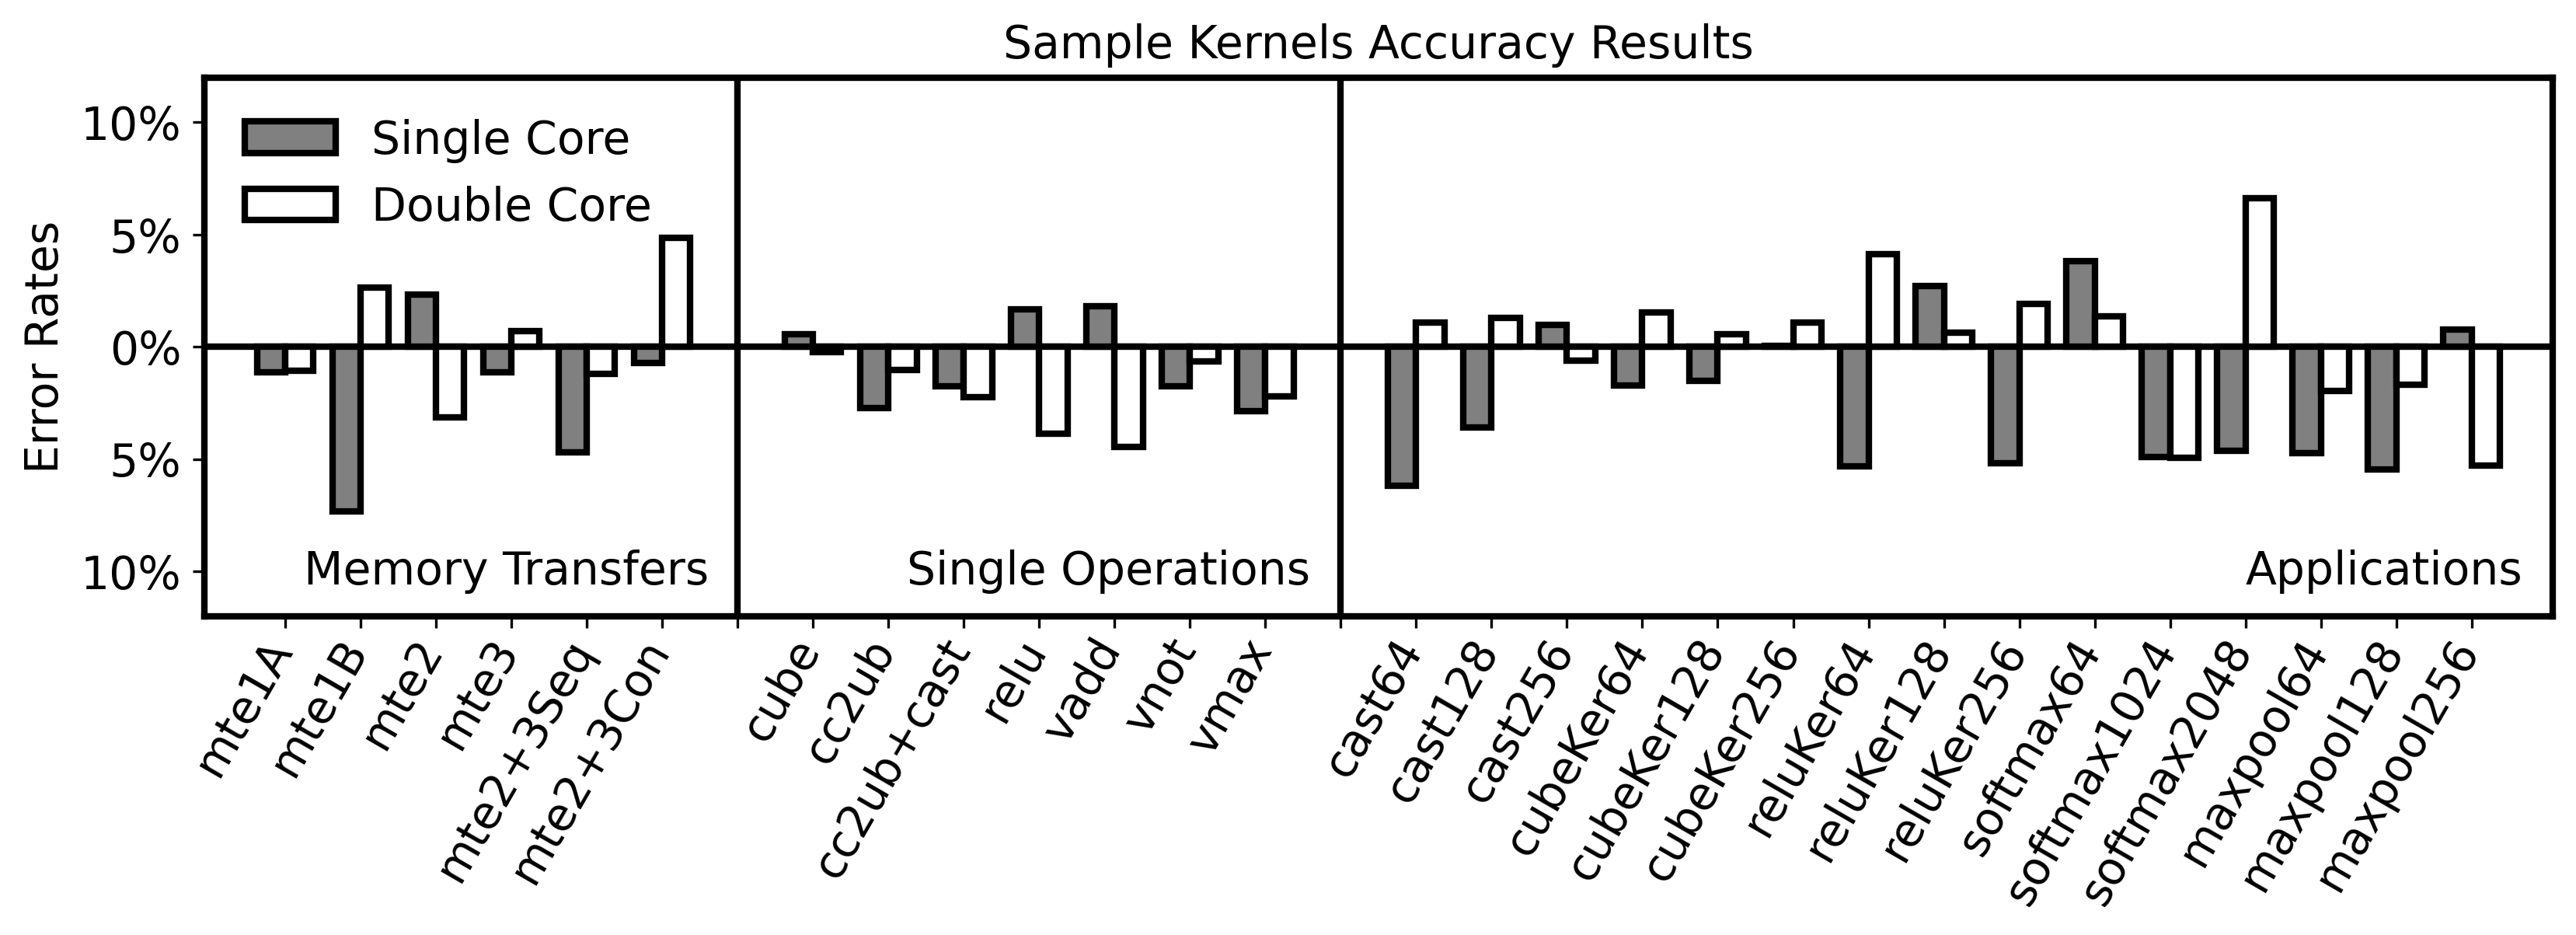
\includegraphics[scale=0.48]{figures/tiny_kernels.png}}
    \captionsetup{justification=centering}
    \caption{The Verrocchio error rate results for sample kernels}
    \label{fig:tiny}
    \end{figure}

\begin{table}[t]
    \caption{Verrocchio sample kernels for accuracy evaluation}
    \label{tab:kernel_type}
    \begin{center}
    
    \scalebox{0.72}{
        \begin{tabular}{c|c|c}    
        \toprule[1pt]
        \textbf{Categories} & \textbf{Kernel Name} & \textbf{Description} \\
        \midrule[0.5pt]

        \multirow{6}*{Memory transfers} & mte1A & Transfer data from L1 Buffer to L0A Buffer \\
        ~ & mte1B & Transfer data from L1 Buffer to L0B Buffer \\
        ~ & mte2 & Transfer data from external storage to L1 Buffer \\
        ~ & mte3 & Transfer data from Unified Buffer to external storage\\
        ~ & mte2+3Seq & MTE2 and MTE3 Units execute sequentially \\
        ~ & mte2+3Con & MTE2 and MTE3 Units execute concurrently \\
        \midrule[0.5pt]
        \multirow{7}*{Single computations} & cube & Do a matrix multiplication w/ Cube Unit\\
        ~ & cc2ub & Transfer from L0C Buffer to Unified Buffer w/ Vector Unit \\
        ~ & cc2ub+cast & Same as above plus type conversion\\
        ~ & relu & ReLU activation function \\
        ~ & vadd & Vectorized addition\\
        ~ & vnot & Vectorized boolean NOT operation\\
        ~ & vmax & Vectorized element-wise Max operation\\
        \midrule[0.5pt]
        \multirow{5}*{\makecell[c]{Applications \\ (Full kernels \\ with I/O)}} & castXxx & Type conversion operator \\
        ~ & cubeKerXxx & Matrix multiplication operator without tiling \\
        ~ & reluKerXxx & ReLU activation operator\\
        ~ & softmaxXxx & Softmax operator\\
        ~ & maxpoolXxx & MaxPooling operator\\
    
        \bottomrule[1pt]
        \end{tabular}
    }
\end{center}
\end{table}
    
\subsection{Matrix Multiplication Optimizing Process}

This section demonstrates an optimizing process of matrix multiplication with Verrocchio, one of the most significant applications for AI processors.

\begin{algorithm}[tbp]
    \caption{Target Improved Matrix Multiplication}
    \label{alg:mat}
    
    \SetKwInOut{Input}{input}
    \SetKwInOut{Output}{output}
    
    \Input{
        matrix \textbf{A}, \textbf{B} of size ($\textit{m} \times \textit{k}$), ($\textit{k} \times \textit{n}$) \\
        % matrix  of size  \\
        tiling parameter \textit{mTiles}, \textit{kTiles}, \textit{nTiles}, \textit{bNum}
    }
        
    \Output{
        matrix \textbf{C} of size ($\textit{m} \times \textit{n}$)
    }
    \BlankLine
    
    % \CommentSty{\# Compute the size of each tile} \\
    (\textit{mSlice}, \textit{kSlice}, \textit{nSlice}) $\leftarrow$ (\textit{m}, \textit{k}, \textit{n}) $/$ 
        (\textit{mTiles}, \textit{kTiles}, \textit{nTiles}) \\
    % \CommentSty{\# Direction Order M $\rightarrow$ N $\rightarrow$ K} \\
    \For{$i \leftarrow 0, j \leftarrow 0$ \KwTo \textit{mTiles}, \textit{nTiles}}{
            \For{$l \leftarrow 0, bf \leftarrow 0$ \KwTo \textit{kTiles} $/$ \textit{bNum}, \textit{bNum}}{
                    \If{$j = 0$}{
                        load \textbf{A} tile \emph{$mSlice \times kSlice$} to \textit{L1} from \textit{External} \tcp*{MTE2}
                    }
                    load \textbf{A} tile \emph{$mSlice \times kSlice$} to \textit{L0A} from \textit{L1} 
                    \tcp*{MTE1}
                    
                    \If{$i = 0$}{
                        load \textbf{B} tile \emph{$kSlice \times nSlice$} to \textit{L1} from \textit{External} \tcp*{MTE2}
                    }
                    load \textbf{B} tile \emph{$kSlice \times nSlice$} to \textit{L0B} from \textit{L1} 
                    \tcp*{MTE1}
                    do matrix multiplication of \textbf{A} tile $\times$ \textbf{B} tile to \textit{L0C} 
                    \tcp*{Cube}
            }
            % \CommentSty{\# Done the K direction} \\
            load \textbf{C} tile \emph{$mSlice \times nSlice$} to \textit{UB} from \textit{L0C} 
            \tcp*{Vector}
            load \textbf{C} tile \emph{$mSlice \times nSlice$} to \textit{External} from \textit{UB} 
            \tcp*{MTE3}
    }
\end{algorithm}

\subsubsection{Improved Matrix Multiplication and Tiling Parameter Selection}

Alg. \ref{alg:mat} shows the target improved matrix multiplication algorithm for optimization. The matrix multiplications require four tiling parameters, \textit{mTiles}, \textit{kTiles}, \textit{nTiles}, and \textit{bNum}, which represents the tile number from the $m$, $k$, and $n$ directions with the multiple control flow number. 

\begin{figure}[tbp]
    \centering{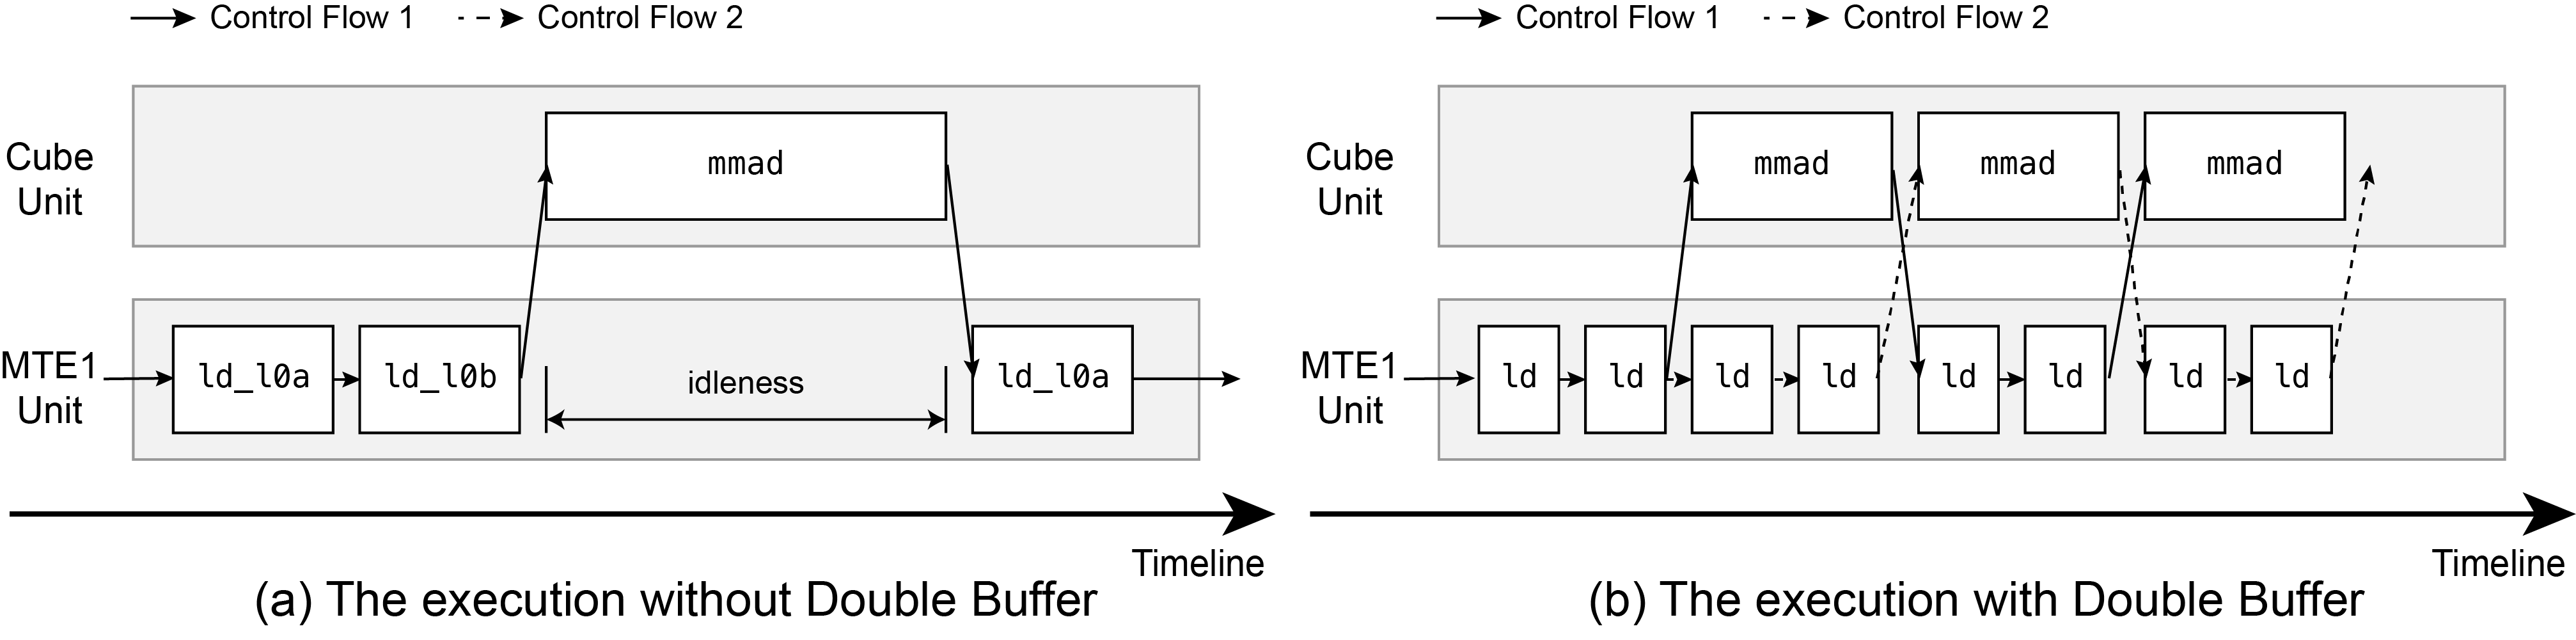
\includegraphics[scale=0.355]{figures/double_buffer.png}}
    \captionsetup{justification=centering}
    \caption{The effect of Double Buffer policy on the execution performance and concurrency}
    \label{fig:doubleb}
    \end{figure}

The matrix multiplication adopts a policy called Double Buffer or Ping-Pong Buffer, shown in Alg. \ref{alg:mat} line 3. DaVinci Core buffers allow reading and writing on different addresses at the same buffer concurrently. Meanwhile, the binary semaphore mechanism allows at most eight independent control flows. Hence, the Double Buffer policy splits the buffers and the operations in half and activates the second control flow. Fig. \ref{fig:doubleb} illustrates how the Double Buffer policy fills the idleness gap of the MTE1 Unit to increase the concurrency and ILP. However, the Double Buffer policy sometimes introduces too much cost and lowers the performance because of the imbalanced execution period.

To formulate an optimization problem, we conduct the tiling parameter selection procedure as a permutation of all four parameters, which are the variables of the problem. The improved matrix multiplication has no further requirements or constraints for the variables, but the tiling numbers must be less than the $16 \times 16 \times 16$ block numbers along the same direction. For each parameter combination in the feasible domain, Verrocchio predicts the execution time and records, which performs the objective function of the optimization problem. To solve the problem, we implement the exhaustive search, the most straightforward solution. Finally, we find the optimized solution as the parameter combination with the least execution time for our matrix multiplication.

\subsubsection{Verrocchio Accuracy Results}

\begin{figure}[tbp]
\centering{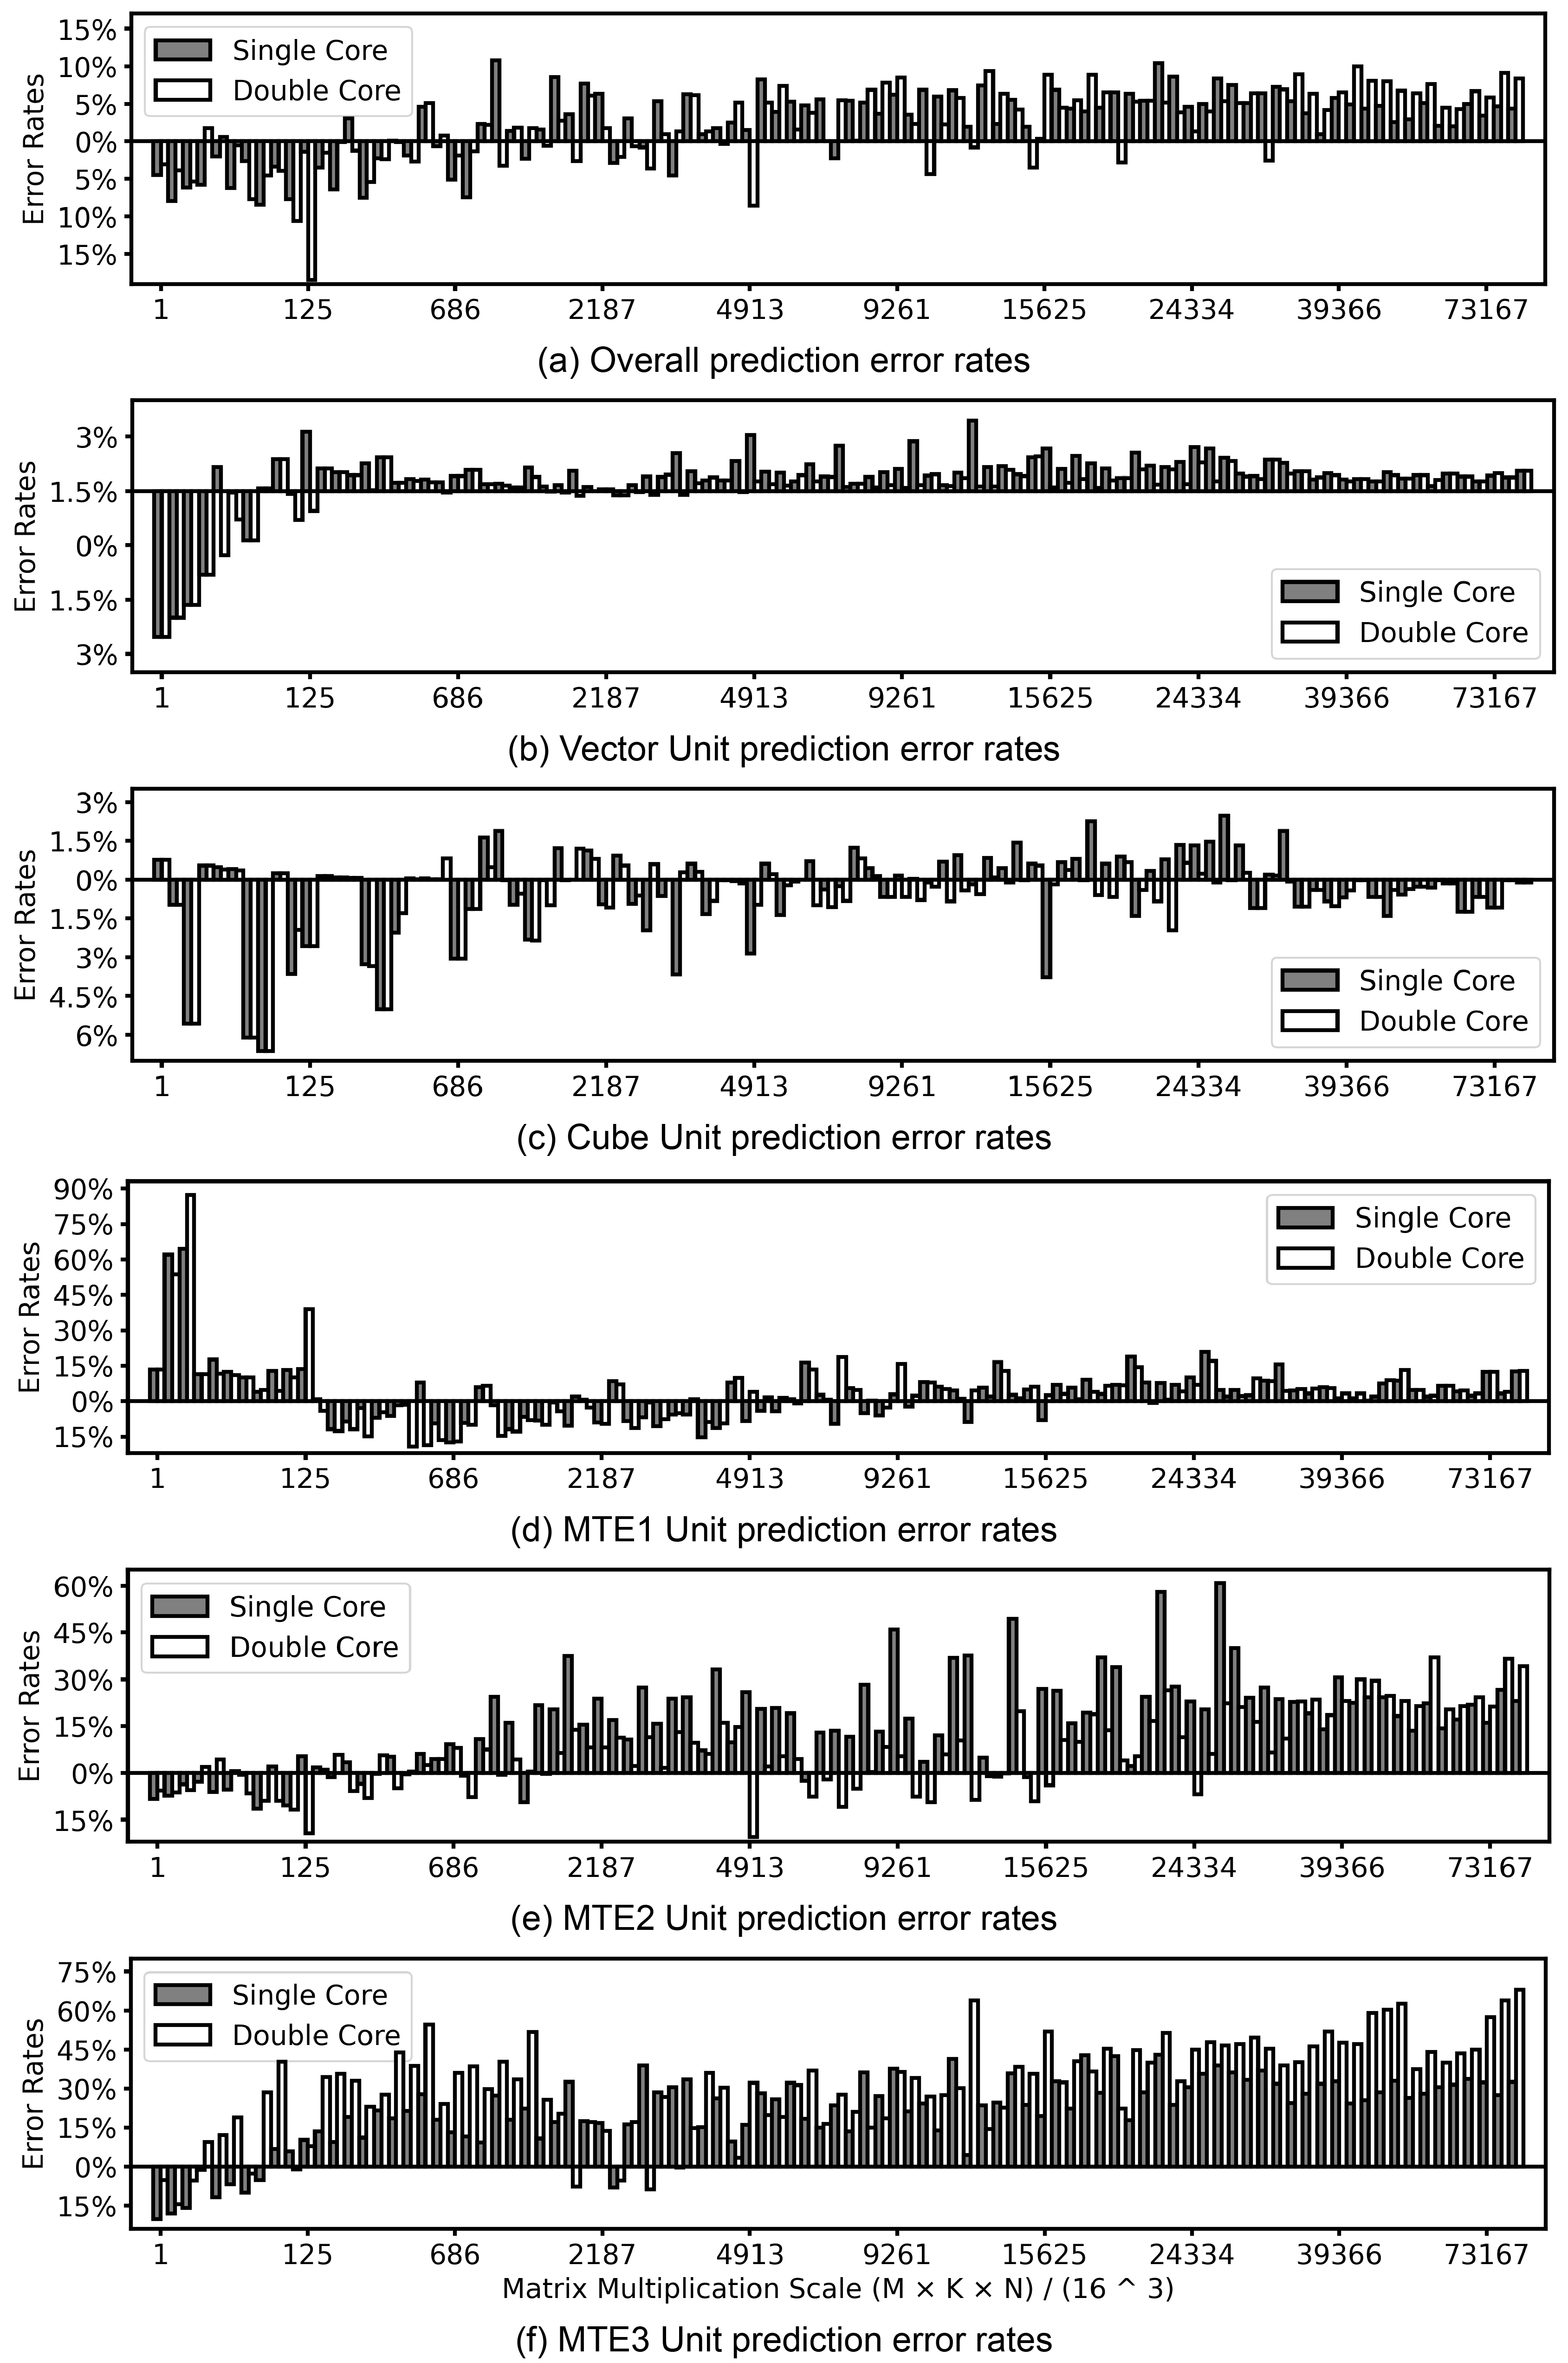
\includegraphics[scale=0.40]{figures/matrixmul.png}}
\captionsetup{justification=centering}
\caption{The Verrocchio error rate results for the improved matrix multiplications}
\label{fig:sim}
\end{figure}

To evaluate the Verrocchio accuracy, we compare our predicted results from Verrocchio with the practical execution time results, which adopt the optimized tiling parameters, as shown in Fig. \ref{fig:sim}. For a better visibility, we define the matrix multiplication scale as the number of the basic blocks operated by the Cube Unit $(m \times k \times n / 16 ^ 3)$. As some matrix multiplications can have the same matrix multiplication scale, we use the average values as the results.

Fig. \ref{fig:sim} (a) shows the total execution time error rates. The average error rate among all test cases is $5.06\%$ for the single-core execution and $5.25\%$ for the double-core execution. The predicted results are lower than the experiment results when the scale is small. One of the potential reasons is that we do not consider the Scalar Unit and the corresponding instructions in Verrocchio. As we discussed in Sec. \ref{sec:ben_des}, the Scalar instructions could block the execution of other units. When the scale gets larger, the effect of the Scalar instructions declines apparently, and the error rates rise above the baseline. When the scale is larger than 5000, the error rates get stable at around 5\%, meaning the prediction of Verrocchio is more accurate and stable in large-scale cases. 

We also show their prediction error rate for each hardware unit separately in the following figures of Fig. \ref{fig:sim}. The Vector Unit and the Cube Unit are well-predicted, reporting the average error rates of $0.69\%$ and $1.17\%$ for the single-core execution, $0.51\%$ and $0.85\%$ for the double-core execution, shown in Fig. \ref{fig:sim} (a) and (b) respectively. The MTE1 Unit performs slightly worse with the average error rates of $9.78\%$ and $9.46\%$. We observe apparent error rates when the scale is small. One of the potential reasons is that the initialization time of the MTE1 instruction is less than other instructions. The MTE2 and MTE3 Units report the worst average error rates of $18.89\%$ and $23.72\%$ for the single-core execution, $14.22\%$ and $33.72\%$ for the double-core execution. Furthermore, the two MTE Units report a system error when the scale is large, where the predicted execution time is always larger than the practical experiment time, especially the MTE3 Unit results. One of the reasons is that, as shown in Fig. \ref{fig:micro_view}, the bus contentions of the MTE Units do not start immediately but wait for the finish of a block. Verrocchio considers all contentions starting at once when the instructions are called, which brings more contentions than the practical execution. In addition, we notice the two MTE Units perform worse in the double-core execution. According to the data collected in Table \ref{tab:bench}, the two DaVinci Cores of the Ascend 310 processors are not synchronized perfectly. Therefore, Verrocchio could bring false contentions in the double-core execution when two respective MTE Units on two cores do not fully overlap.

\subsubsection{Matrix Multiplications Acceleration Results}

\paragraph{Operator Level}

\begin{figure}[tbp]
\centering{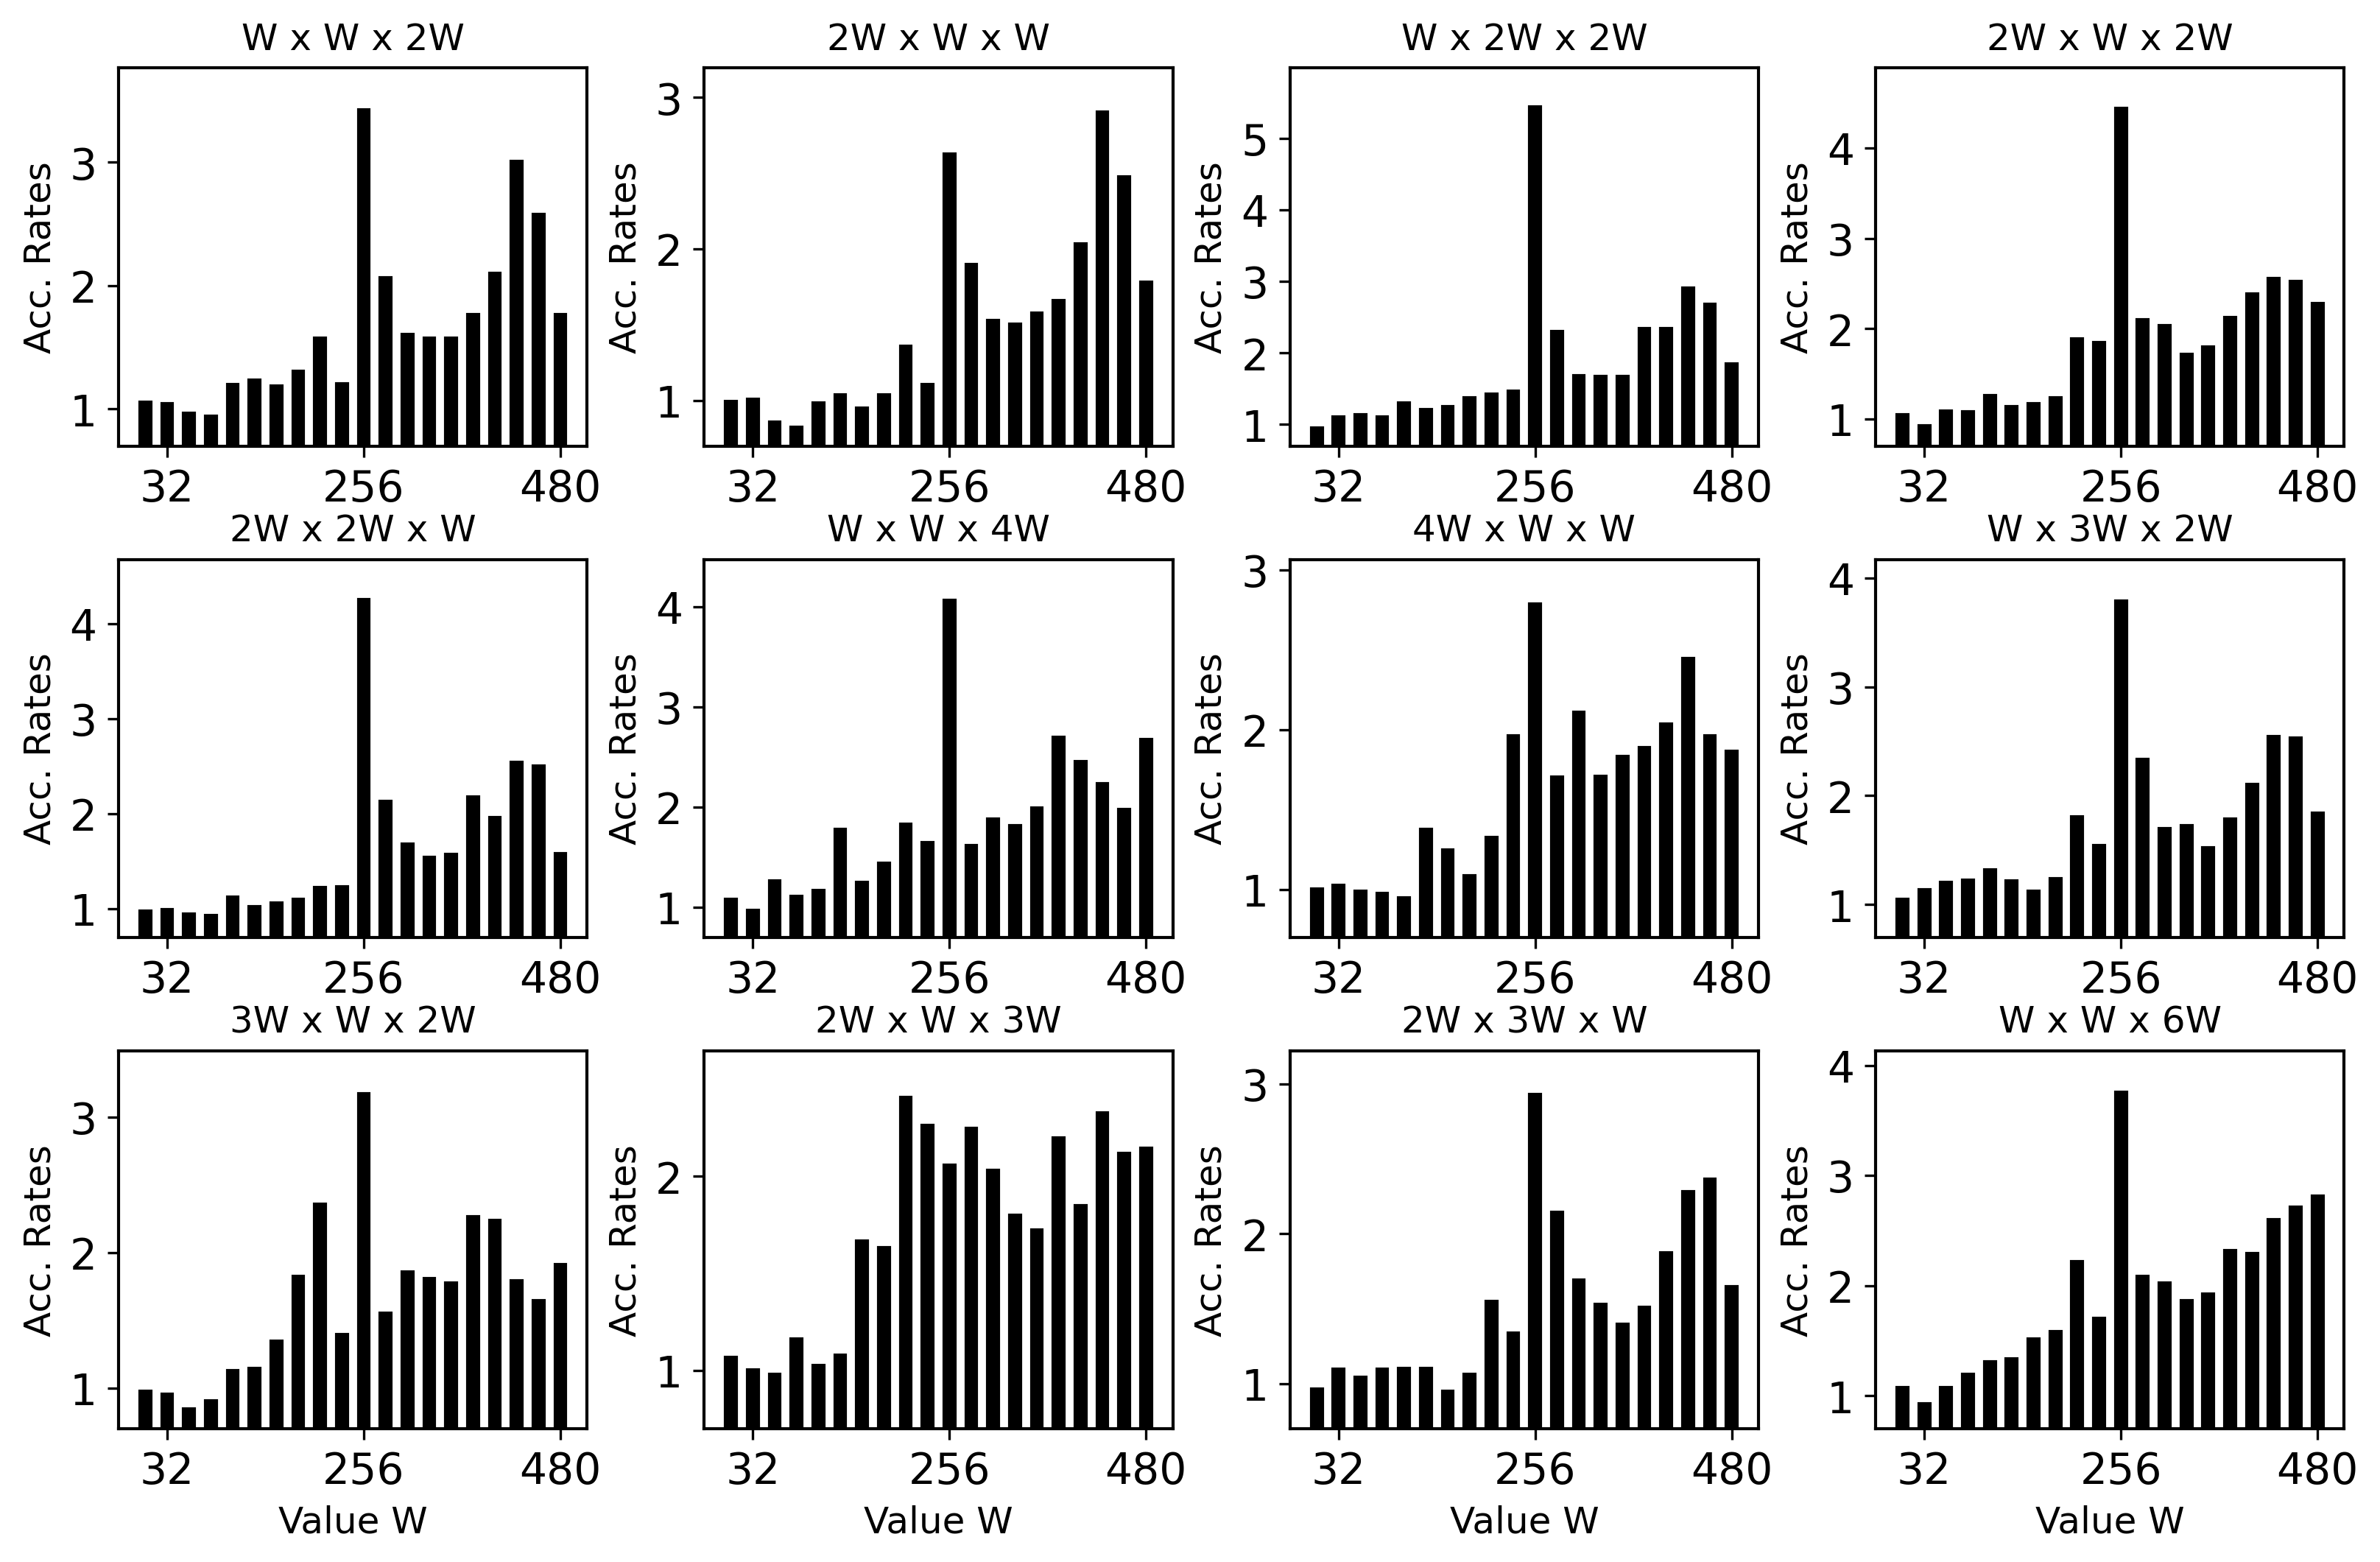
\includegraphics[scale=0.5]{figures/eva.png}}
\caption{Accelerations of the improved matrix multiplication compared with the CANN operators}
\label{fig:eva}
\end{figure}

We compare the improved matrix multiplications with the Huawei CANN operators. As the CANN operators require different logical core numbers, we keep the active core numbers as their respective demands. Our improved matrix multiplication always uses two cores, so we set the core number to two during the experiments of our algorithm. We test matrix multiplications in 12 shapes, from $W \times W \times 2W$ to $W \times W \times 6W$, as shown in Fig. \ref{fig:eva}.

The results show how Verrocchio helps the matrix multiplications to achieve a significant speedup. The improved matrix multiplications achieve an average speedup of 1.70$\times$ among all test cases compared with the Huawei official CANN operators. Generally, the accelerations grow steadily with the increment of the matrix multiplication scale (or value W). For the regular-shaped matrix multiplications like $W \times W \times 2W$, our matrix multiplications show similar performance compared with the CANN operators, where the two approaches follow similar tiling strategies. However, our matrix multiplications perform much better for those irregular-shaped matrix multiplications like $W \times W \times 4W$. The main reason is that the CANN operators abuse the multiple logical cores with inefficient tilings in these irregular-shaped cases, even when the Ascend 310 processors have only two physical cores. Meanwhile, our improved matrix multiplications focus on the two physical DaVinci Cores with the most appropriate and efficient tilings suggested by Verrocchio, which make great improvements.

Furthermore, we plot our matrix multiplications in the roofline model \cite{DBLP:journals/cacm/WilliamsWP09}, as shown in Fig. \ref{fig:roofline}, which considers the Cube Unit FLOPS and the bandwidth between the L0 and L1 Buffer. Compared with the CANN operators, our matrix multiplication algorithm reports a smaller performance gap to the attainable roofline results. The average ratio of the peak hardware performance we achieve is 23.64\%, 2.09X higher than that of the CANN operators. With the increment of the operation intensity, the ratio of our algorithm becomes higher than that of the CANN operators, and finally stops at about 38.78\%, which further proves the better performance in larger scales we observed in Fig. \ref{fig:eva}.

\begin{figure}[tbp]
    \centering{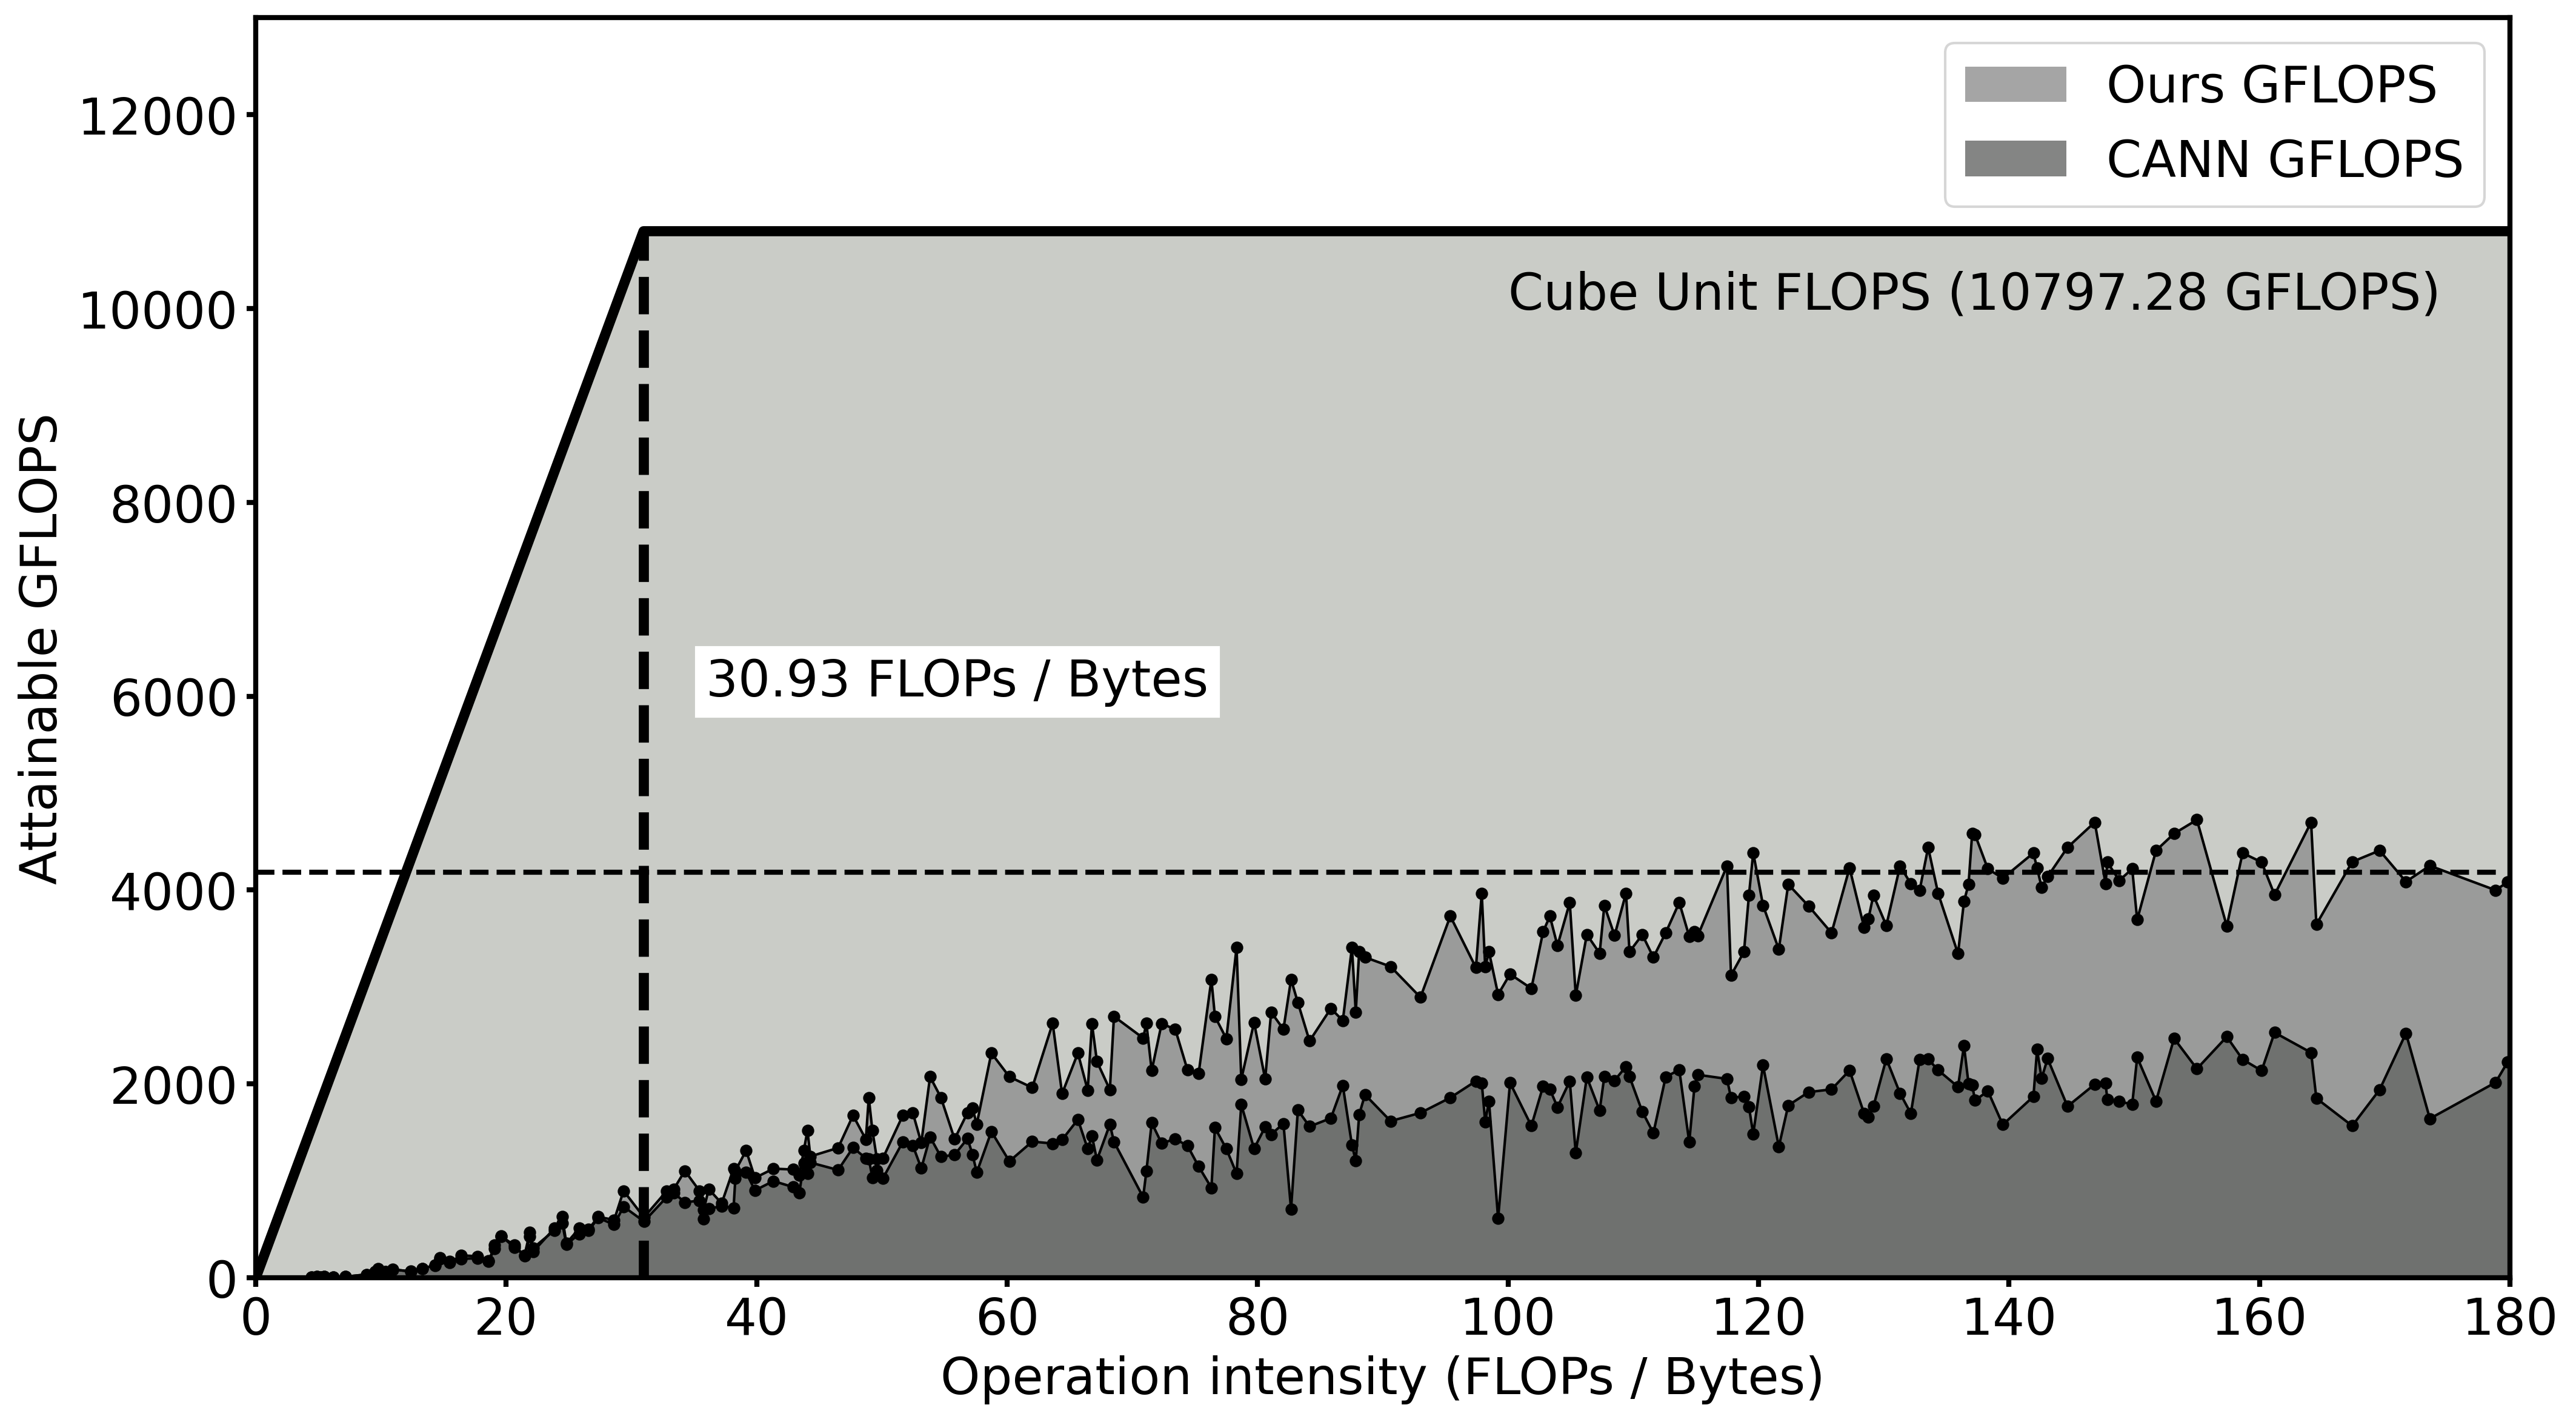
\includegraphics[scale=0.36]{figures/roofline_comp.png}}
    \caption{The roofline model with the matrix multiplication results annotated}
    \label{fig:roofline}
    \end{figure}

\begin{figure}[tbp]
    \centering{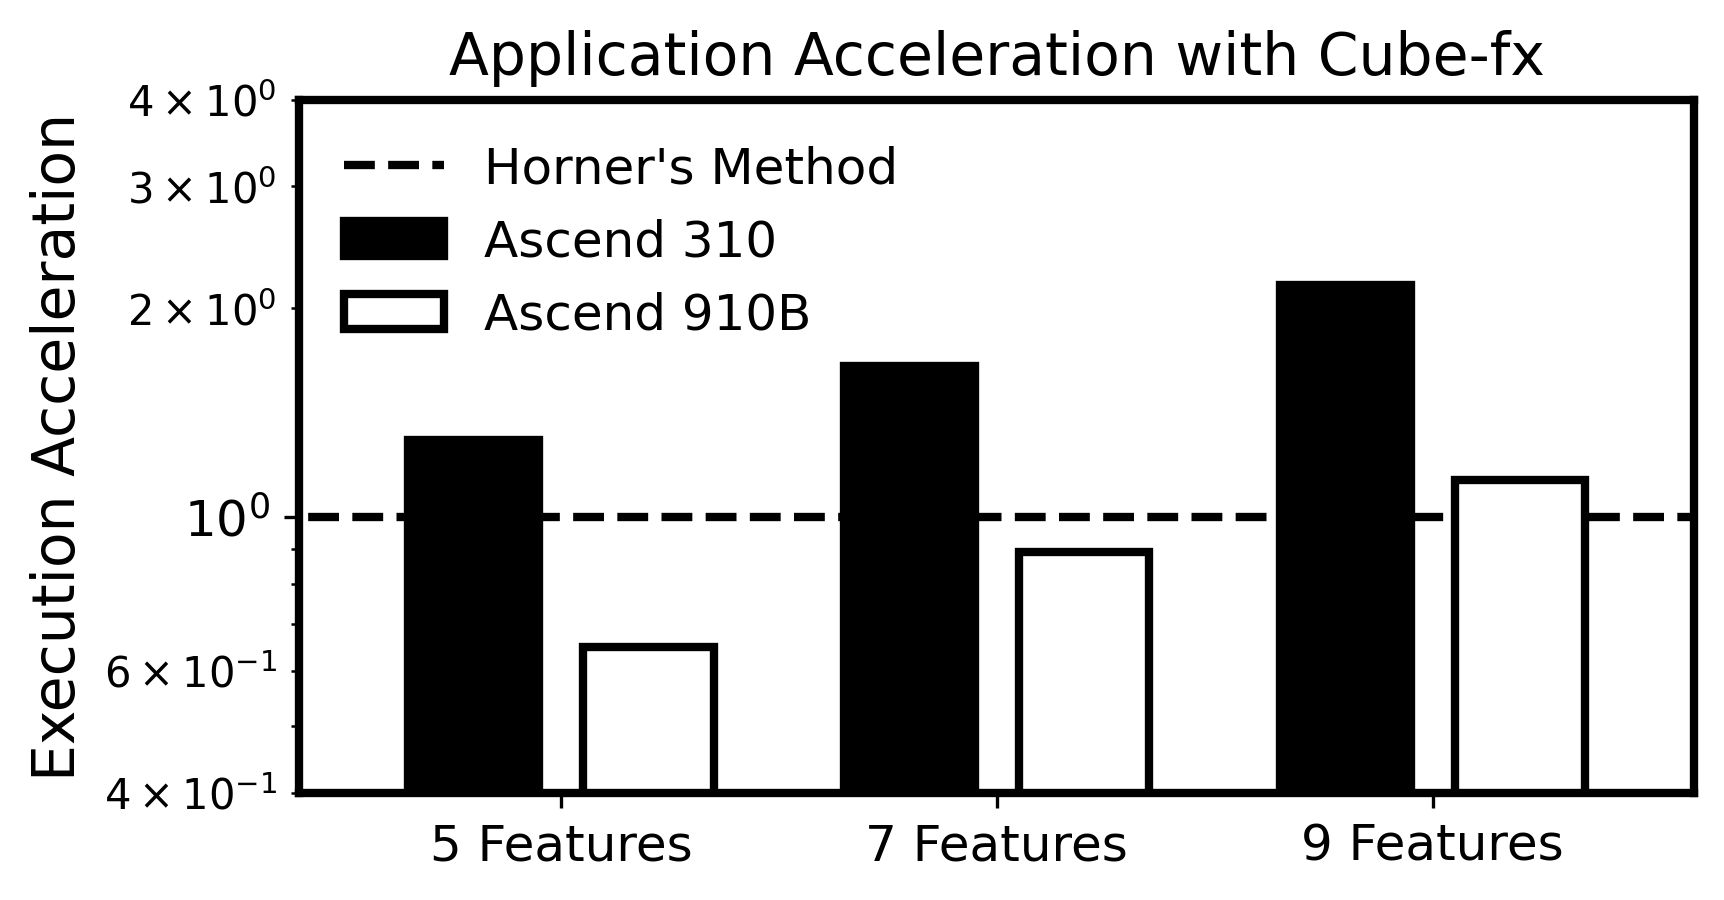
\includegraphics[scale=0.55]{figures/app_acc.png}}
    \caption{The estimation results of the popular DNN applications}
    \label{fig:app_acc}
    \end{figure}
        
\paragraph{Application level}

Currently, executing a DNN model on Ascend 310 processor needs an official ATC offered by Huawei, which converts the Caffe or TensorFlow model to the Huawei custom model. However, Huawei does not offer the structures and formats of the custom model. Hence, we propose an estimated method to evaluate the acceleration brought by the improved matrix multiplications for popular DNN applications. For each layer of a DNN application, we evaluate the total execution time and the Cube Unit execution time. We compute the matrix multiplication scales defined in the last subsection with the collected Cube Unit execution time. Therefore, with the average acceleration rates of the scale, we have an approximate acceleration result of this matrix multiplication operator. By estimating all operators, we have final results of the DNN application \cite{DBLP:conf/cvpr/HeZRS16, DBLP:journals/corr/abs-2004-10934, DBLP:conf/cvpr/SandlerHZZC18, DBLP:conf/nips/KrizhevskySH12, DBLP:conf/naacl/DevlinCLT19}, as shown in Fig. \ref{fig:app_acc}.

Among all evaluation results, AlexNet shows the most significant speedup of 2.18$\times$. The reason is that AlexNet is one of the earliest Convolutional Neural Networks (CNNs) with large Fully Connected (FC) layers. It requires matrix multiplications of a large scale. As we show in the last subsection, the CANN operators perform worse than our operators on a large scale. Generally, the DNN applications report an average speedup of 1.53$\times$. Although YOLO V4 is a complex model, the matrix multiplication scales are not large, reporting the lowest acceleration rate of 1.15$\times$.

\section{Conclusion and Future Work}

For the first time, we focus on building a performance model, Verrocchio, for Huawei DaVinci AI Cores. The DaVinci Core has complex data paths and distinct working details, which significantly influences the performance and brings a series of modeling challenges. Our discrete-event-based model reports high accuracy for various kernel programs but involves some system errors of the MTE Unit bandwidths, which are caused by the simplification of their runtime behaviors. In future work, we plan a deeper study with more benchmarks of the MTE Units, which aims to model the accurate bandwidth contentions.

%========================================

\chapter{SelB-k-NN: Replacing the Worst Operations}
\label{sec_3}

\section{Background \& Motivation}

\subsection{\textit{K}-Nearest Neighbors Algorithm}

\textit{K}-NN is one of the most classical and well-studied algorithms for classification problems. The general idea of \textit{k}-NN is uncomplicated: those points in the same category mostly have high similarity and are located close to one another in high-dimensional space. To classify a test point, \textit{k}-NN computes the similarity between the test point and all the training points and then selects the \textit{k} nearest neighbors in the \textit{k}-selection phase. \textit{K}-NN finally chooses the category of the most neighbors in the \textit{k} nearest neighbor results as the test point's category.

In the early days, the distance computation took most of the \textit{k}-NN's execution time. With the improvement of the hardware, GPUs with massive parallelism successfully mitigate the bottleneck. The \textit{k}-selection phase remains a new bottleneck with several solutions. In general, the \textit{k}-selection algorithms are divided into two categories, heap-based \cite{DBLP:conf/medi/VelentzasVC21, DBLP:conf/sigmod/ShanbhagPM18, DBLP:conf/ccgrid/KatoH10, DBLP:journals/concurrency/KatoH12, DBLP:conf/icip/GarciaDNB10, DBLP:conf/egh/LiSPAOA12} and bitonic-based \cite{DBLP:conf/sigmod/ShanbhagPM18, DBLP:journals/tbd/JohnsonDJ21, DBLP:conf/ipps/Tang0EMG15}. However, the two approaches rely on a considerable number of weakly supported operations on the AI processors. For 16-selection of 16 test points with 4096 training points on the Huawei Ascend 310 processors, the dynamic addressing during sibling selections in the re-heap procedure occupies 94.10\% of the heap-based \textit{k}-selection execution time. The vectorized comparisons \& selections, which support compare-and-swap operations, occupy 75.98\% of the bitonic-based \textit{k}-selection. A novel algorithm to reduce these operations on the AI processors is urgently needed.

\subsection{Tiling Shape Mismatch of \textit{K}-NN \label{sec:tiling}}

Tiling is an effective technique for matrix multiplication optimization, which benefits from the data locality and is widely studied on the different platforms including the AI processors \cite{DBLP:conf/ppopp/Li0YJL19, DBLP:conf/ppopp/NiuLJS0022, DBLP:conf/ppopp/HongSNSS19, DBLP:conf/ipps/00020C20, DBLP:conf/ppopp/FengWCZ0D21, DBLP:conf/micro/ZhaoD20}. It combines sufficient knowledge of the hardware structures and the fixed specific matrix multiplication execution patterns for maximized hardware performance.

However, most of their works separate the matrix multiplications from the applications. While the matrix multiplications prefer regular tiling shapes ($m \approx n$) on the matrix MACs \cite{DBLP:conf/ipps/00020C20}, \textit{k}-selections prefer irregular ones ($m \gg n$) on the vector units, which brings a tiling shape mismatch. For example, the heap-based \textit{k}-selection is expanded efficiently along the $m$-direction, maintaining $m$ heaps on the vector units for parallel element-wise comparison. Increasing $m$ would not prolong the execution time seriously, while increasing $n$ raises the loop iterations and makes the execution longer. However, the matrix multiplication output restricts the $k$-selection's tiling shape. When selecting a regular tiling shape for the matrix multiplication, the relation $m \gg n$ cannot be true for the \textit{k}-selection. On other platforms, selecting the regular tiling shapes for $k$-NN may perform well. On AI processors, the matrix multiplication does not dominate the $k$-NN execution time. Directly applying matrix multiplication's tiling shapes works poorly on the $k$-selection and harms the $k$-NN performance.


\section{SelB-k-NN Algorithm}

\begin{figure}[t]
    \centering{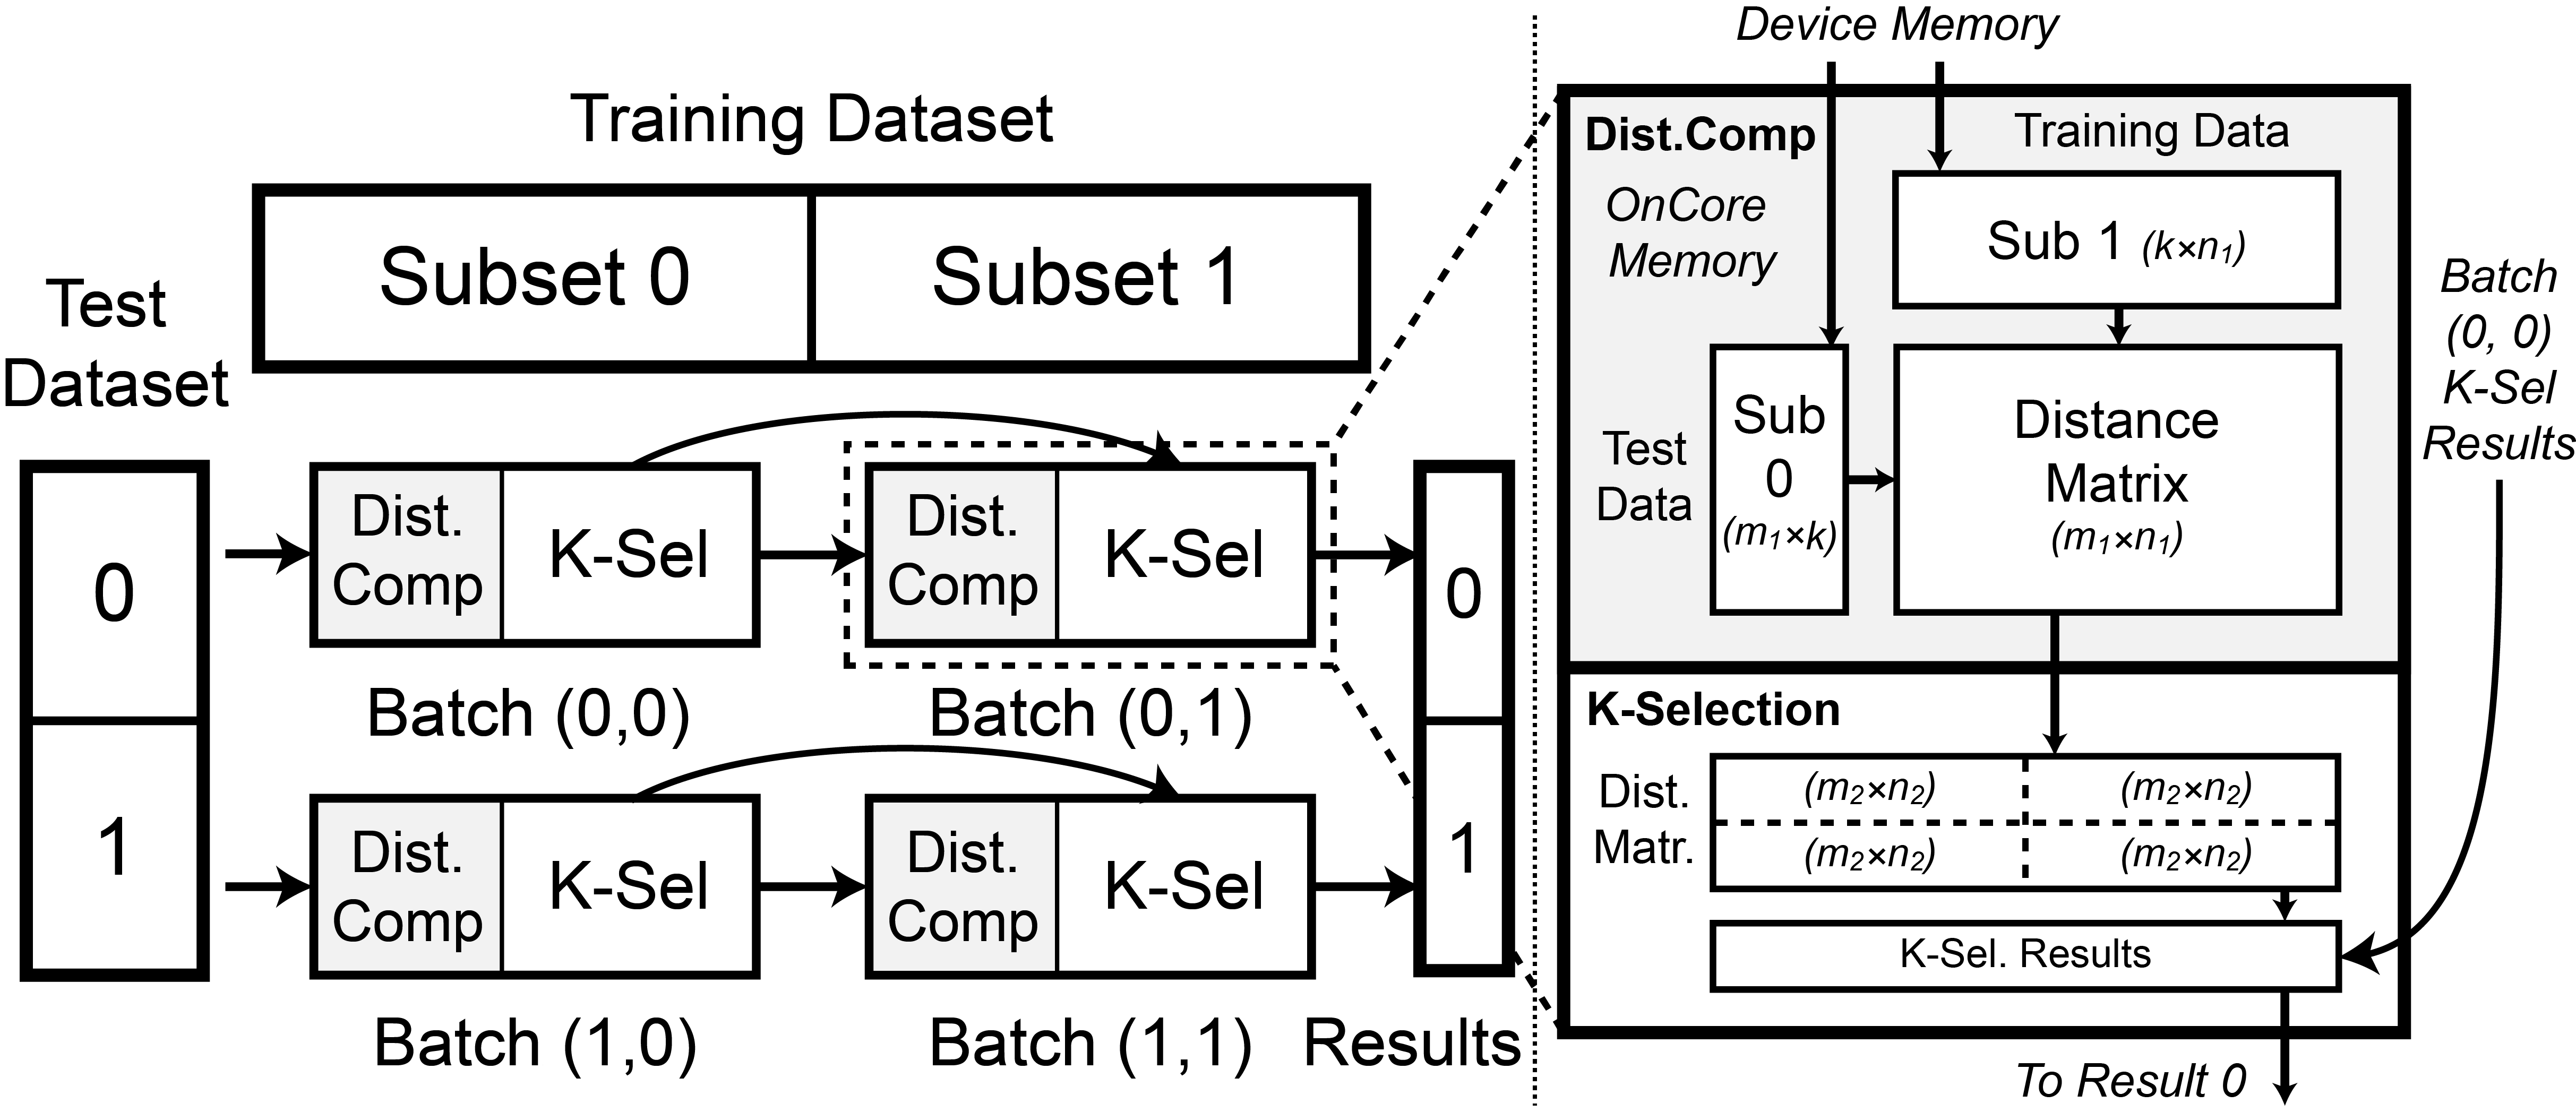
\includegraphics[scale=0.3]{figures/tiling.png}}
    \caption{An overview of SelB-\textit{k}-NN with a detailed view of the batch (0, 1)}
    \label{fig:tiling}
    \end{figure}

Fig. \ref{fig:tiling} illustrates an overview of SelB-\textit{k}-NN. It first tiles the test and training datasets along the $m$-direction and $n$-direction respectively. A batch is assigned a tile of the workload with the distance computation tiling shape $(m_1, n_1)$. It receives data from the datasets, computes and updates the previous min-\textit{k} results from the last adjacent batch along the $n$-direction. The \textit{k}-selection of each batch is further tiled with the tiling shape $(m_2, n_2)$, as shown on the right side of Fig. \ref{fig:tiling}. The processed data of each batch is transferred from the large but slow device memory, while the intermediate min-\textit{k} results can be maintained constantly at the fast but tiny on-core memory until the finish of the current test dataset tile along the $m$-direction. The mini-batches are executed sequentially on a single processor and easily applied to multi-processors \cite{van2007superlinear}. This section mainly describes a single batch of SelB-\textit{k}-NN.

\subsection{Distance Computation on AI Processors}

By accelerating the matrix multiplications with the matrix MACs, the AI processors efficiently improve the performance of cosine distance computations. 

The cosine distance of points $\boldsymbol{p}_{1}, \boldsymbol{p}_{2}$ is:

\begin{equation}
    \label{eq:cosine}
    \begin{aligned}
    D_{cos} = 1 - \frac{\boldsymbol{p}_{1} \cdot \boldsymbol{p}_{2}}
            {\left\| \boldsymbol{p}_{1} \right\| 
                \left\| \boldsymbol{p}_{2} \right\|}
        = 1 - \boldsymbol{p}_{1} \cdot \boldsymbol{p}_{2}\  (\textnormal{for } \ell\textnormal{2-norm pts.})
    \end{aligned}
    \end{equation}

Therefore, the essence of the distance computation is the dot product of two vectors. For $m_1 \times n_1$ data, we compute the dot products following the matrix multiplication below:

\begin{equation}
    \label{eq:dot_products}
    \begin{aligned}
    \begin{bmatrix} 
        \boldsymbol{p}_{1} \\
        \vdots \\
        \boldsymbol{p}_{m_1}
    \end{bmatrix}
    \cdot
    \begin{bmatrix} 
        \boldsymbol{q}_{1}^{T} &
        \dots &
        \boldsymbol{q}_{n_1}^{T}
    \end{bmatrix}
    =
    \begin{bmatrix} 
        \boldsymbol{p}_{1} \cdot \boldsymbol{q}_{1} &
        \dots &
        \boldsymbol{p}_{1} \cdot \boldsymbol{q}_{n_1} \\
        \vdots & \ddots & \vdots \\
        \boldsymbol{p}_{m_1} \cdot \boldsymbol{q}_{1} &
        \dots &
        \boldsymbol{p}_{m_1} \cdot \boldsymbol{q}_{n_1} \\
    \end{bmatrix}
    \end{aligned}
    \end{equation}

where $\boldsymbol{p}_{i}$ and $\boldsymbol{q}_{i}$ are $d$ dimensional vectors. For simplicity, we assume that all the data in this work are $\ell$2-normalized, and the term \textit{distance} in the paper is cosine distance.

\subsection{\textit{K}-Selection on AI Processors}

SelB-\textit{k}-NN \textit{k}-selection algorithm relies on two groups of common vector operations, which are used in the most significant operations in DNN applications and supported by AI processors \cite{CANN, jax, cambricon}. The first includes \verb|reduceMin| (and \verb|reduceMax|), which find the minimized value in a given vector. Some AI processors further support returning the corresponding indices \cite{CANN}. The two operations form the central part of the pooling layer, frequently used after convolutional layers. The other includes \verb|vecCmp| and \verb|vecSel|, which compare two given vectors by elements to build a mask and select the elements based on the mask. The two operations support an elementary branch for data, which is necessary for training like the backpropagation computation of \verb|ReLU|. However, as discussed, existing works \cite{DBLP:conf/icpp/JiW21, cambricon, CANN} indicate inefficiency or lack of the two operations on some AI processors.

Our \textit{k}-selection algorithm finds indices of the min-\textit{k} results for $m_2$ separate $n_2$-sized vectors in at most $k$ steps. For each vector, the general idea is to ensure that after the \textit{k}-selection phase, the minimum value remaining in the vector is greater than the maximum value in the min-\textit{k} results. Based on the idea, we propose the \textit{k}-selection algorithm in Alg. \ref{alg:single_main}.

\begin{algorithm}[tbp]
    \caption{SelB-\textit{k}-NN \textit{K}-Selection Algorithm}
    \label{alg:single_main}
        
    \SetKwInOut{Input}{Input}
    \SetKwInOut{Output}{Output}
        
    \Input{
        distance matrix \textbf{D} of size ($\textit{m}_2 \times \textit{n}_2$) \\
        last min-$k$ results \textbf{K} of size ($\textit{k} \times \textit{m}_2$) \\
        last indices of results \textbf{I} of size ($\textit{k} \times \textit{m}_2$)
    }
            
    \Output{
        min-$k$ results \textbf{K}$^{\prime}$ of size ($\textit{k} \times \textit{m}_2$) \\
        indices of results \textbf{I}$^{\prime}$ of size ($\textit{k} \times \textit{m}_2$)
    }
    \BlankLine
    
    $mask \leftarrow$ $\vec{\textbf{0}}$ \\
        
    \For{$step \leftarrow 0$ \KwTo $k$}{
        \For{$ln \leftarrow 0$ \KwTo $m$}{
            \If{$mask[ln] \neq 0$}{
                \textbf{continue}
            }
            $(res_{min}, idx_{min})[ln] \leftarrow$ \textbf{reduceMin}$(\textbf{D}[ln])$ \\
            $\textbf{D}[ln][idx_{min}[ln]] \leftarrow +\infty$ \tcp*{Scalar}
        }
        $cmp \leftarrow$ \textbf{vecCmpLt}$(res_{min}, \textbf{K}[0])$ \tcp*{Cmp}
        $mask \leftarrow$ \textbf{vecSel}$(cmp, mask, \vec{\textbf{1}})$ \tcp*{Sel}
        $mask_{min} \leftarrow$ \textbf{reduceMin}$(mask)$ \\
        \If{$mask_{min} \neq 0$}{
            \Return \textbf{K} as \textbf{K}$^{\prime}$, \textbf{I} as \textbf{I}$^{\prime}$
        }
        $\textbf{K}[0] \leftarrow$ \textbf{vecSel}$(cmp, res_{min}, \textbf{K}[0])$ \tcp*{Sel}
        $\textbf{I}[0] \leftarrow$ \textbf{vecSel}$(cmp, idx_{min}, \textbf{I}[0])$ \tcp*{Sel}
        $\textbf{bitonicKSel}(\textit{k} = 1, (\textbf{K}, \textbf{I}))$ \tcp*{O(\textit{k}) Cmp\&Sel}
    }
    \Return \textbf{K} as \textbf{K}$^{\prime}$, \textbf{I} as \textbf{I}$^{\prime}$
\end{algorithm}

\begin{figure}[tbp]
    \centering{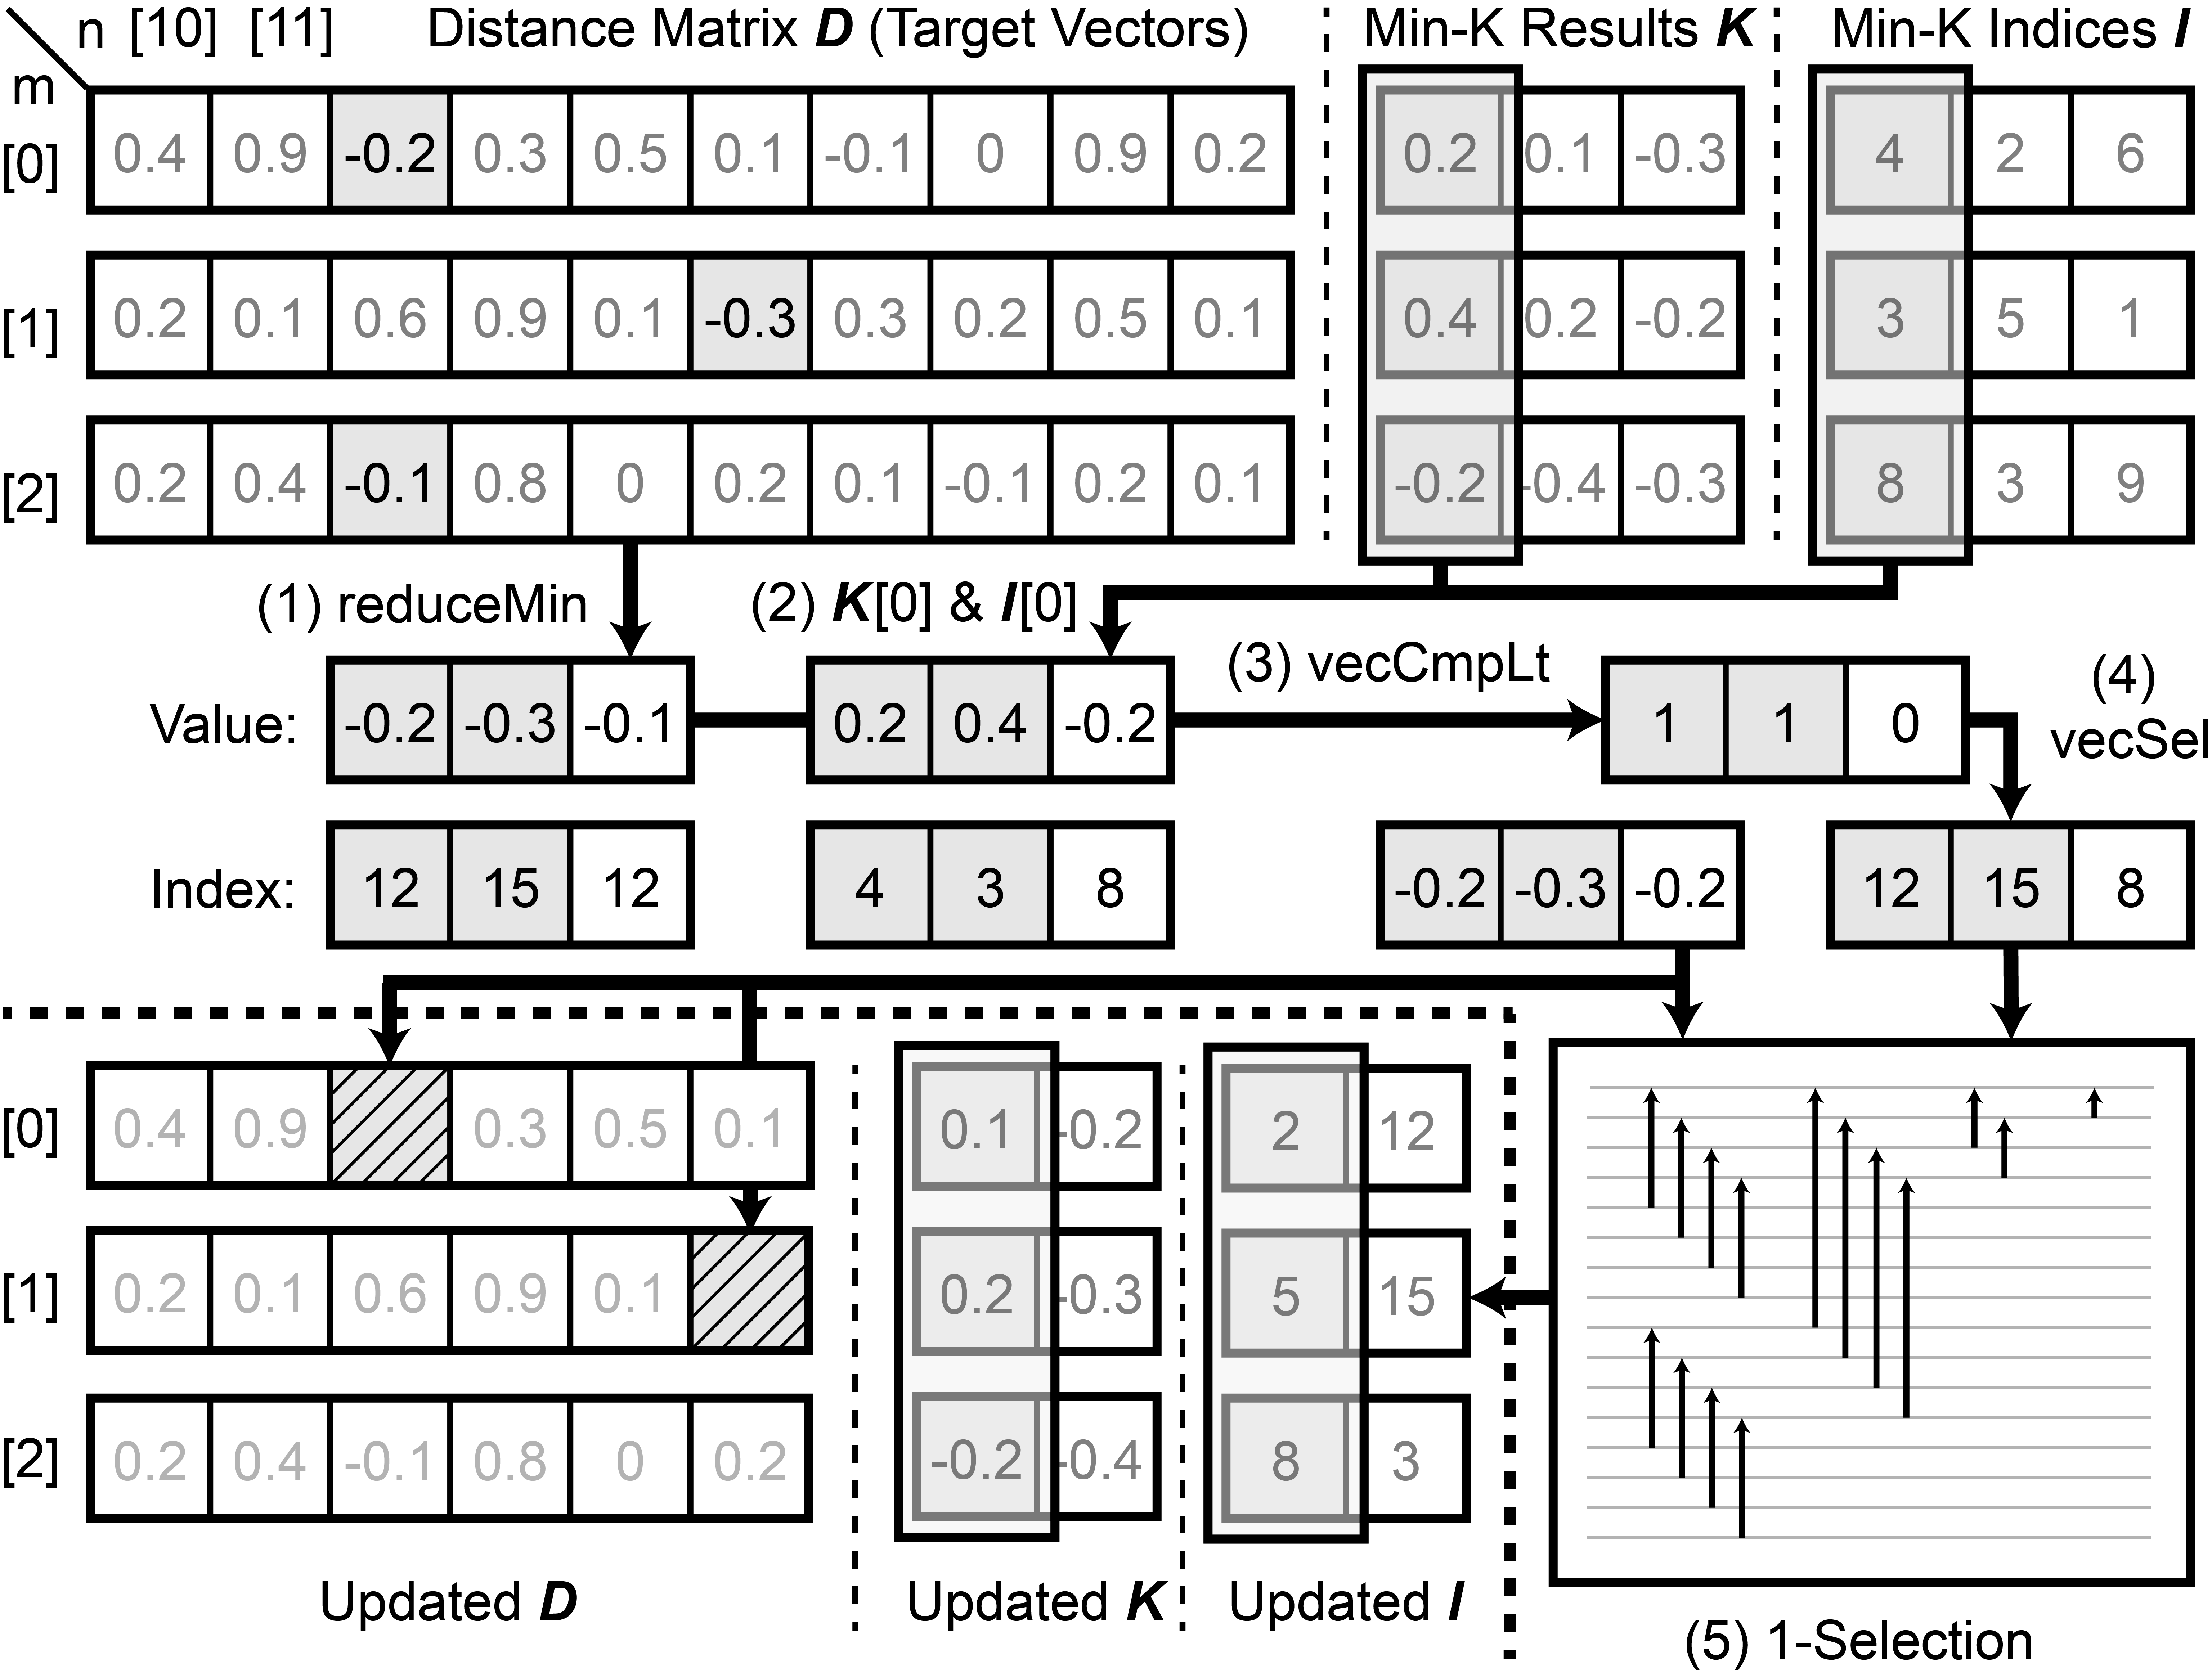
\includegraphics[scale=0.23]{figures/single_k_sel.png}}
    \caption{One step of the batch $(0, 1)$ of the \textit{k}-selection ($m_2 = 3, n_2 = 10$)}
    \label{fig:single_k_sel}
    \end{figure}

The main procedure of the algorithm is a \textit{k}-step loop. Fig. \ref{fig:single_k_sel} illustrates one \textit{step} example of the batch $(0, 1)$ of the \textit{k}-selection with the tiling shape of $m_2 = 3, n_2 = 10$, which process the data range of $m \in [0, 3), n \in [10, 20)$. The algorithm first find the minimum value $res_{min}$ with its index $idx_{min}$ in the target vector $\textbf{D}[ln]$. Then for $m$ target vectors, we compare whether $res_{min}$ is less than the first element of the min-\textit{k} results $\textbf{K}[0]$ in parallel. With the compared results, we update $\textbf{K}[0]$ and $\textbf{I}[0]$ accordingly. For the example in Fig. \ref{fig:single_k_sel}, $\textbf{K}[0][0]$ and $\textbf{K}[0][1]$ are updated since $-0.2 < 0.2$ and $-0.3 < 0.4$. The next step is the most significant step, where we maintain the min-\textit{k} results $\textbf{K}$ to ensure the first element is always the maximum element with the bitonic 1-selection. When $k=1$, the bitonic \textit{k}-selection is degenerated to a reduction but not only return the reduced value as \verb|reduceMax| does. Instead, it rearranges the vector and puts the top-$1$ value at the first element. Compared with directly invoking \verb|reduceMax|, the bitonic 1-selection avoids scalar dynamic addressing that locates the reduction results and variable assignments that update values for each target vector respectively. Instead, it calls $O(k)$ vectorized comparisons \& selections. On the other hand, the approach should not replace \verb|reduceMin| for the $n$-sized $\textbf{D}$, which would bring $O(n)$ vectorized comparisons \& selections as the direct bitonic-based approach does for the entire \textit{k}-selection. With the compared results, we also update value $res_{min}$ in the target vector with a large constant. 

For each test point, the time complexity of SelB-\textit{k}-NN \textit{k}-selection algorithm is $O(k + k^2 + nk)$, which consists of three parts, the scalar operation part, the vectorized comparison \& selection part, and other well-supported vector operation part. Although the overall time complexity seems to be higher than the heap-based \textit{k}-selection of $O(nlogk)$ and the bitonic-based \textit{k}-selection of $O(nlog^2k)$, our algorithm significantly reduces the scalar operations from $O(nlogk)$ to $O(k)$, and the vectorized comparisons \& selections from $O(nlog^2k)$ to $O(k^2)$, as annotated in Alg. \ref{alg:single_main}. SelB-\textit{k}-NN \textit{k}-selection algorithm prevents the less powerful operations of AI processors from growing with the scale of training dataset $n$. Existing works \cite{hassanat2014solving, abu2019effects} report that in \textit{k}-NN algorithm, a larger parameter \textit{k} does not contribute to higher accuracy. Therefore, we can safely assume that $n \gg k$, where our algorithm restrains the number of the scalar operations and vectorized comparisons \& selections for higher performance with acceptable accuracy.

The second feature of the algorithm is an early exit policy. For $m_2$ test points, we initialize an $m_2$-length vector $mask$ to '0's. The vector is updated each step based on the parallel comparison results by selecting the elements between $mask$ itself with '1's, as shown in line 10. All the values of those target vectors, whose minimum values are greater than the maximum values in their corresponding min-\textit{k} results, are greater than all the values in the min-\textit{k} results, as Eq. \ref{eq:main_equation} shows. 

\begin{equation}
    \label{eq:main_equation}
    \begin{aligned}
    \forall x \in \textbf{D}, res_{min} \le x &;\ 
        \forall y \in \textbf{K}, res_{max} \ge y \\
    res_{min} > res_{max} &\implies \forall x > \forall y
    \end{aligned}
\end{equation}

Therefore, once $res_{min} > res_{max}$, all the remaining values in the target vector are not the candidates of the min-\textit{k} results and can be rejected directly. Then the related element of $mask$ is updated to '1', and the algorithm skips the corresponding target vector, as shown in line 4. In the example of Fig. 3, the $\textbf{D}[2]$ is rejected in this step since $-0.1 > -0.2$. When the minimum value of $mask$ is not '0', which means all the elements are updated to '1', the algorithm ends in advance, as shown in line 11. For all batches after tiling the test dataset along \textit{m}-direction and the training dataset along \textit{n}-direction, each batch of SelB-\textit{k}-NN additionally receives the min-\textit{k} results from the last adjacent tile along \textit{n}-direction, as shown in \textbf{Input K} of Alg. \ref{alg:single_main}. The early exit policy can be activated by the last results and reduces most workloads during the execution. We will discuss the details of the workload reduction later in Sec. \ref{sec:tile}.

\section{Minimizing Hardware Support Requirements}

To minimize the hardware support as much as possible for portability of SelB-\textit{k}-NN, this section proposes two algorithms to replace the uncommon functions in DNNs with the most common functions on the AI processors \cite{cambricon, CANN, jax}.

\subsection{ReLU-Based Operations for VecCmp and VecSel \label{sec:relu}}

For the AI processors without \verb|vecCmp| and \verb|vecSel| hardware supports, we propose a novel \verb|ReLU|-based bitwise algorithm specifically for the AI processors. We do not involve bit-shifting or integer division to avoid extra requirements for hardware components on the AI processors.
    
\begin{algorithm}[tbp]
    \caption{Bitwise Ops for VecCmpLt and VecSel}
    \label{alg:bit_hack}
            
    \SetKwInOut{Input}{Input}
    \SetKwInOut{Output}{Output}
            
    \Input{
        compared vector \textbf{A, B} of FP16 numbers \\
        target vector \textbf{X, Y} of 16-bits numbers \\
    }
                
    \Output{
        result vector \textbf{R} from \textbf{X} and \textbf{Y}, based on the element-wise minimum between \textbf{A} and \textbf{B}
    }
    \BlankLine
    \#\# \textbf{VecCmpLt:} Computing \textit{mask} from \textbf{A, B} \\
    $\text{sub}_{1} \leftarrow \textbf{A} - \textbf{B}$ \\
    $\text{sub}_{2} \leftarrow (\text{sub}_{1} \  \& \  \vec{\textbf{0x8000}}) \mid \vec{\textbf{0x0001}}$ \\
    $\text{mask}_{1} \leftarrow \textbf{ReLU}(\text{sub}_{2})$ \\
    $\text{mask}_{2} \leftarrow \text{reinterpret} \  \text{mask}_{1} \  \text{as INT16 vector}$ \\
    $\text{mask} \leftarrow \text{mask}_{2} - \vec{\textbf{1}}$ \\
    
    \BlankLine
    \#\# \textbf{VecSel:} Computing \textbf{R} with \textit{mask} from \textbf{X, Y}\\
    $\textbf{R} \leftarrow \textbf{X} \ \&\ \text{mask}$ \\
    $\textbf{R} \leftarrow \textbf{R} \mid (\textbf{Y} \ \&\ \sim \text{mask})$ \\
\end{algorithm}
    
We show the algorithm in Alg. \ref{alg:bit_hack} for \verb|vecCmpLt| and \verb|vecSel|, which generates a mask based on the smaller elements of the two vectors and then selects values from the other two target vectors with the mask. For any vector \textbf{A} and \textbf{B}, Alg. \ref{alg:bit_hack} first computes the the vectorized subtraction results $sub_{1}$. Then it masks out the exponent and mantissa part (last 15 bits) of the FP16 number $sub_{1}$ and then sets the last bit to '1' by a bitwise inclusive OR operation. For the element where $A < B$, the $sub_{2}$ is 0x8001, while for $A > B$, the $sub_{2}$ is 0x0001. The essence and the most novel part of the algorithm is line 3, where it computes the comparison mask $mask_{1}$ with \verb|ReLU|, which is one of the most representative activation functions. The binary form of \verb|ReLU| function is shown below:

\begin{equation}
    \label{eq:relu}
    \textbf{ReLU}(t) = \left\{
    \begin{aligned}
        &\text{0b0xxx}  &t = \text{0b0xxx} \  &(t \ge 0) \\
        &\text{0b0000} &t = \text{0b1xxx} \  &(t \le 0) \\
    \end{aligned}
    \right.
\end{equation}
    
where 'x' is any bit ('0' or '1'). For both floating-point and integer numbers, whose most significant bit (the 1st bit) is the sign bit, \verb|ReLU| checks the sign bit and returns the result values according to its formula. Therefore, after line 3, the $mask_{1}$ for $A < B$ is set to 0x0000, while for $A > B$ it is set to 0x0001. Alg. \ref{alg:bit_hack} reinterprets $mask_{1}$ as INT16 number, which requires no instructions but only indicates that the following operation is integer operations. Then Alg. \ref{alg:bit_hack} subtracts INT16 number 1 from the result following the integer arithmetic rules. After that, the final comparison mask $mask$ for $A < B$ becomes 0xffff ($-1$ in INT16), while for $A > B$, it becomes 0x0000. To compute the mask of $A > B$ (vecCmpGt), swap the input $\textbf{A}$ and $\textbf{B}$ and the rest part remains the same. For the mask of $A = B$ (vecCmpEq), the $sub_{1}$ is modified to be computed by the formula below with other parts unchanged:

\begin{equation}
    sub_{1} \leftarrow (\textbf{A} - \textbf{B}) \mid (\textbf{B} - \textbf{A})
\end{equation}

With the comparison masks, Alg. \ref{alg:bit_hack} then selects the values from the target vector \textbf{X} and \textbf{Y}. Line 6 masks the values in \textbf{X} vector where $A > B$ with the corresponding mask of 0x0000, and keeps values where $A < B$ with the mask of 0xffff. Line 7 finishes the symmetric jobs and combines the two results with a bitwise inclusive OR operation.

The replaced \verb|vecCmpLt| and \verb|vecSel| involves only several efficient vector operations on the AI processors, including \verb|ReLU|. \verb|ReLU| is innately designed to contain a branch operation but wrapped by its original algorithm. Our algorithm widens \verb|ReLU| with its branch operation to general purposes. The algorithm contains no scalar operations and can achieve high performance on the AI processors.

\subsection{Indexing with Vector Operations}

While \verb|reduceMin| (\verb|reduceMax|) is irreplaceable in the deep learning applications, returning the corresponding indices is not necessary to be supported on the AI processors. To migrate the algorithm to the AI processors without vectorized hardware indexing supports, we propose an efficient algorithm for indexing on those AI processors shown as Alg. \ref{alg:indices_search}. The algorithm has one more vector operation than the \textit{k}-selection algorithm, \verb|vecDup|, which assigns a value to the whole vector and is also commonly used in the initialization of each layer.

\begin{algorithm}[tbp]
    \caption{Indexing w/ Vector Operations}
    \label{alg:indices_search}
        
    \SetKwInOut{Input}{Input}
    \SetKwInOut{Output}{Output}
        
    \Input{
        indexing vector \textbf{K} of size (n) \\
        indexing target value V
    }
            
    \Output{
        index of value V in vector \textbf{K}
    }
    \BlankLine
    
    $\text{idxMap} \leftarrow [0, 1, 2, \dots, (\text{n}-1)]$ \\
    $\text{vArray} \leftarrow [\text{V}, \text{V}, \text{V}, \dots, \text{V}]$ \\
    $\text{cmp} \leftarrow $ \textbf{vecCmpEq}$(\text{vArray}, \textbf{K})$  \\
    $\text{idxArray} \leftarrow $ \textbf{vecSel}$(\text{cmp}, \text{idxMap}, \vec{\textbf{0xfc00}})$ \\
    $\text{V} \leftarrow$ \textbf{reduceMax}$(\text{idxArray})$ \\
\end{algorithm}

The algorithm first assigns the target value $V$ to an $n$-sized array $vArray$ with \verb|vecDup|. Then it compares the $vArray$ with the indexing vector \textbf{K} to build a bitmask with \verb|vecCmpEq| for the position where $V$ locates. With the comparison mask $cmp$, we select the indices data between a prepared indices map $idxMap$ and an array full of 0xfc00 to build a result array $idxArray$. With \verb|reduceMax|, the algorithm finds the result index of indexing target value $V$. Since the indexing algorithm has no scalar operations, it would not be the bottleneck of the whole \textit{k}-selection algorithm.

One tricky part is the value 0xfc00. Most AI processors \cite{DBLP:journals/micro/ChoquetteGGSK21, DBLP:conf/isca/LiuDTHLXCC16, DBLP:conf/isca/JouppiYPPABBBBB17, DBLP:conf/hotchips/LiaoTXZ19} adopt FP16 as the computation data type to save the storage and improve the performance. Therefore, the vector operations usually fully support FP16 data on these AI processors but support INT16 data partially, e.g., subtraction we used in Sec. \ref{sec:relu}. For \verb|vecCmpEq| operations without INT16 data supports, since it does not rely on the numerical value of the data, we can directly cast the INT16 indices data to FP16 with no bit modifications. However, for \verb|reduceMax|, we need to ensure that the final index we find is numerically greater than others in FP16 format. Therefore, we select the value 0xfc00 as the initialized value, which is the negative infinity of FP16 and is less than all other 16-bit data in FP16 format. In this way, when we still cast our INT16 indices data to FP16 without any format conversions, \verb|reduceMax| still works no matter how the bits represent in FP16 format. One potential issue is that when multiple target values $V$ exist in the vector, we cannot ensure which index will be returned. However, it makes no trouble in our \textit{k}-selection algorithm. In addition, on the AI processors that support INT16 vector operations, the value 0xfc00 still works well. The value 0xfc00 is negative in INT16 format (-1023) and less than all possible indices.

\section{Optimal Tiling Shape Search \label{sec:tile}}

As illustrated in Fig. \ref{fig:tiling}, the parameters $(m_1, n_1)$ and $(m_2, n_2)$ determine the tiling (or batch) shapes of the distance computation and the \textit{k}-selection, which significantly influences the entire performance. This section discusses how we find the optimial tiling shapes with an optimization problem.

\subsection{\textit{K}-selection Workload Quantification \label{kSel}}

Along the $n$-direction, while each tile of the matrix multiplications has stable and equal workloads, the workload of each tile in SelB-\textit{k}-NN \textit{k}-selection varies based on its assigned datasets and last min-\textit{k} results. During the runtime of the algorithm, the early exit policy of the \textit{k}-selection is continually activated by the last adjacent tile's results. It dynamically rejects the for-loop steps of the \textit{k}-selection as shown in Alg. \ref{alg:single_main}, identified as the primary workloads. Intuitively, the later tiles always have fewer workloads. To accurately model the algorithm performance to an optimization problem, we present an analysis to quantify the \textit{k}-selection workload of the tile $t$.

Let us assume that for a specific test data $m$, the distance computation results of all training data $D$ obey some random distribution $\mathcal{F}(X)$. Therefore, after the computation of tile $t$ during the execution, the distance computation results that have been computed $D_{1 \to t}$ and are computed just at the computation of tile $t$, $D_{t}$, also obey the distribution $\mathcal{F}(X)$.

\begin{equation}
    \begin{aligned}
        D \sim \mathcal{F}(X) \implies D_{1 \to t}, D_{t} \sim \mathcal{F}(X)  
    \end{aligned}
\end{equation}


Then let us consider that after the tile $t$, $x^{\prime}_{1 \to t}$ is the \textit{k}-th minimum value of $D_{1 \to t}$, which is also the maximum value of the \textit{k}-min results. We can compute the cumulative distribution function (CDF) of the distribution $\mathcal{F}_{X}(x^{\prime}_{1 \to t})$ as follows:

\begin{equation}
    \mathcal{F}_{X}(x^{\prime}_{1 \to t}) = P(X \le x^{\prime}_{1 \to t}) = \frac{k}{nt}
\end{equation}

where $n$ is the number of distance results of each tile (also the number of \textit{k}-selection inputs). The CDF computes the probability of randomly selecting a value from $D_{1 \to t}$, which is one of the \textit{k}-min results. Let us call that for the tile $t$, the values, which belong to the distance results $D_{t}$ and are going to replace another value in the current \textit{k}-min results, are \textit{updating} values. Then for the tile $t$, when one value $x$ is updating at this stage, it means that $x \le x^{\prime}_{1 \to t}$. Therefore, for the tile $t$ of size $n$, the expected number of the updating value can be computed by the CDF as follows:

\begin{equation}
    E_{t}(X \le x^{\prime}_{1 \to t}) = n \mathcal{F}_{X}(x^{\prime}_{1 \to t}) = \frac{k}{t}
\end{equation}


Since each for-loop \textit{step} of SelB-\textit{k}-NN \textit{k}-selection in Alg. \ref{alg:single_main} updates one value, the expected \textit{updating} value is also the expected \textit{step} number for tile $t$. Hence, for tile $t$, the workload of the \textit{k}-selection phase is quantified to $k / t$ theoretically.

\subsection{Execution Time Optimization Problem Formulation}

For the entire test dataset of $(M \times d)$ and the training dataset of $(d \times N)$, let us consider the tiling shape $(m_{1}, n_{1})$ for the distance computation phase and $(m_{2}, n_{2})$ for the \textit{k}-selection phase. As we discussed in Sec. \ref{sec:tiling}, since the tiling shapes of $k$-selection are restricted by those of distance computation, we have $m_{2} \le m_{1}, n_{2} \le n_{1}$. Our goal is to minimize the overall execution time by a space exploration of the four tiling shapes $(m_{1}, n_{1})$ and $(m_{2}, n_{2})$. Formally, we formulate the following optimization problem.

\begin{equation}
    \label{eq:optimized}
    \begin{aligned}
        min\quad  &T_{mm} + T_{kSel} \\
        s.t.\quad &T_{mm} = \frac{MN}{m_{1}n_{1}} f(m_{1}, n_{1}) \\
                  &T_{kSel} = \frac{M}{m_{2}} \sum_{t=1}^{\frac{N}{n_{2}}}(\frac{k}{t}g(m_{2}, n_{2}) + g_{0}(m_{2}, n_{2})) \\
                  &d(m_1 + n_1) + m_2(n_2 + k) < Size_{mem} \\
                  &m_{2} \le m_{1}, n_{2} \le n_{1} \quad \quad (*)
    \end{aligned}
\end{equation}

where $f(m_{1}, n_{1})$ is the profiled execution time of the matrix multiplication with the tiling shape $(m_{1}, n_{1})$, $g(m_{2}, n_{2})$ is the execution time of a \textit{step} in \textit{k}-selection (line 3 to 15 in Alg. \ref{alg:single_main}) with the tiling shape $(m_{2}, n_{2})$ with constant cost $g_{0}(m_{2}, n_{2})$, $Size_{mem}$ is the size the on-core memory.

\subsection{Search Space Pruning}

The search space size of the optimization problem in Eq. \ref{eq:optimized} is $O(m^2n^2)$, which can be very large and time-consuming to search exhaustively. This subsection adds one more constraint to prune its search space to $O(m^2n)$.

For the optimized solutions, the search procedure contains a four-layer loop to search the parameters. It firsts select a set of $(m_{1}, n_{1})$ in the outer loops, and then traverse all $(m_{2}, n_{2})$ in the inner loops with the constraint $(*)$. At the innermost loop for $n_{2}$ search, while $(m_{1}, n_{1}, m_{2})$ are selected, let we consider $pn_{2} = n_{1}$, where $p \ge 1$. Then we have:

\begin{equation}
    \begin{aligned}
        T_{kSel}(m_{2}, n_{2}) = 
            \frac{M}{m_{2}} \sum_{t=1}^{\frac{pN}{n_{1}}}(\frac{k}{t}g(m_{2}, \frac{n_{1}}{p}) + g_{0}(m_{2}, \frac{n_{1}}{p}))
    \end{aligned}
\end{equation}

If $T_{kSel}(m_{2}, n_{2}) > T_{kSel}(m_{2}, n_{1})$ always holds, it means that for any $p > 1$ (or for any $n_{2} < n_{1}$), the execution time is longer compared with the exeuction time when $n_{2} = n_{1}$. Therefore, let us consider:


\begin{equation}
    \begin{aligned}
        T_{kSel}(m_{2}, n_{2}) &> T_{kSel}(m_{2}, n_{1}) \\
        \sum_{t=1}^{\frac{pN}{n_{1}}}(\frac{k}{t}g(\frac{n_{1}}{p}) + g_{0}(\frac{n_{1}}{p})) &> \sum_{t=1}^{\frac{N}{n_{1}}}(\frac{k}{t}g(n_{1}) + g_{0}(n_{1}))
    \end{aligned}
\end{equation}

where we simplify $g(m_{2}, n)$ to $g(n)$. Then we have:


\begin{equation}
    \label{eq:ineq}
    \begin{aligned}
        \frac{N}{n_{1}}(pg_{0}(\frac{n_{1}}{p}) - g_{0}(n_{1})) + k &(\sum_{t=1}^{\frac{pN}{n_{1}}}\frac{g(\frac{n_{1}}{p})}{t} - \sum_{t=1}^{\frac{N}{n_{1}}}\frac{g(n_{1})}{t}) > 0
    \end{aligned}
\end{equation}

Notice that:


\begin{equation}
    \begin{aligned}
        k (\sum_{t=1}^{\frac{pN}{n_{1}}}\frac{g(\frac{n_{1}}{p})}{t} - \sum_{t=1}^{\frac{N}{n_{1}}}\frac{g(n_{1})}{t}) > - k \sum_{t=1}^{\frac{N}{n_{1}}}\frac{g(n_{1})}{t} > - \frac{kN}{n_{1}} g(n_{1})
    \end{aligned}
\end{equation}

Then Eq. \ref{eq:ineq} is converted to:


\begin{equation}
    \label{eq:last}
    \begin{aligned}
        pg_{0}(\frac{n_{1}}{p}) - (&g_{0}(n_{1}) + kg(n_{1})) > 0
    \end{aligned}
\end{equation}

Since the inequality above does not involve input $N$, after profiling the execution time (e.g., $g(n_{1})$) on the AI processors, the search space can be reduced in advance in the preprocessing stage. For a set of selected $(m_{1}, n_{1}, m_{2})$, when $n_{2}$ satisfies the inequality above, the search for $n_{2}$ should be pruned directly as $n_{1} = n_{2}$. In addition, the inequality can be explained qualitatively. It suggests that for \textit{k}-selection with the tiling shape $n_{1}$, we further divide $n_{1}$ into $p$ smaller tiling shapes $n_{2}$. If the constant cost of the $p$ smaller tiling shapes' execution time ($pg_{0}(\frac{n_{1}}{p})$) is larger than the maximum execution time of the original tiling shape $n_{1}$ ($g_{0}(n_{1}) + kg(n_{1})$), the division of the $p$ tiles is ineffective.

\begin{figure}[htbp]
    \begin{adjustbox}{addcode={
        \begin{minipage}{\width}}{
            \caption{The single execution results of several \textit{k}-NN algorithm kernels}
            \label{fig:single}
        \end{minipage}},rotate=90,center}
        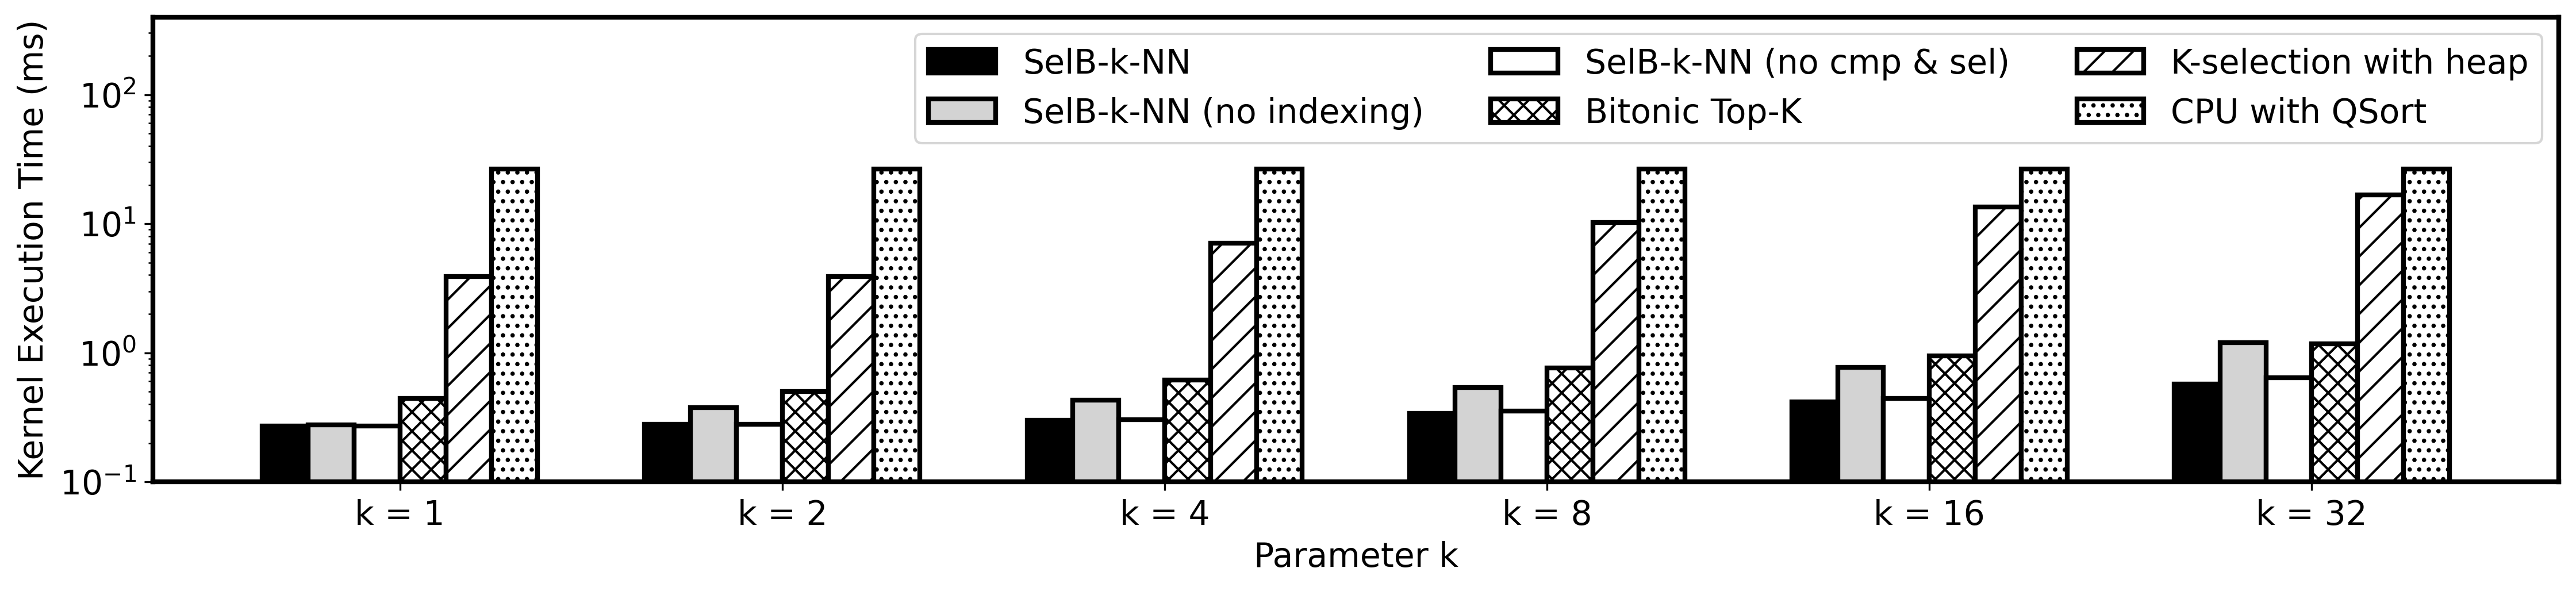
\includegraphics[scale=0.5]{figures/single_core.png}
    \end{adjustbox}
\end{figure}

\section{Evaluation}

We implement SelB-\textit{k}-NN algorithm on Huawei Ascend AI processors based on DaVinci \cite{DBLP:conf/hotchips/LiaoTXZ19} architecture for evaluation. The essence of the Ascend AI processors is DaVinci AI Cores, which provide 4 TFLOPS (FP16) or 8 TOPS (INT8) computation power per core. In addition to the hardware, Huawei also introduced a full-stack programming framework called AI Heterogeneous Compute Architecture (CANN) \cite{CANN}. We program all experiments with Tensor Boost Engine (TBE) and Tensor Iterator Kernel (TIK) for DaVinci kernel programming on CANN. For the matrix multiplication phase, we directly use the official native functions in CANN libraries. The detailed hardware model we used is the Huawei Ascend 310 processor (two DaVinci AI Cores installed) with 2 vCPUs of Intel Cascade Lake 6278 2.6GHz. All experiment results are wall-clock execution period from the start of the distance computation kernel to the end of the \textit{k}-selection kernel (or the end of \textit{k}-selection computation in the CPU approaches). For the evaluation dataset, since SelB-\textit{k}-NN is insensitive to the data distribution, we build randomly generated synthetic datasets. The data points are 128-dimensional with the value of each dimension in the range of $[-1, 1]$ on normal distribution.

\subsection{Single Execution of SelB-k-NN}

We compare SelB-\textit{k}-NN with the bitonic \textit{k}-selection approach, heap-based approach on the AI processors, and host CPU C++ STL quick sort approach. The distance computations of all approaches are accelerated by the Matrix MACs. We offer the implementation results without hardware indexing and \verb|vecCmp| \& \verb|vecSel| supports for the SelB-\textit{k}-NN algorithm. Fig. \ref{fig:single} shows the results of the test cases where the size of the test dataset is $(32 \times 128)$, and the size of the training dataset is $(128 \times 4096)$. We analyze the performance changes with the variation of the parameter \textit{k} of \textit{k}-NN.

\subsubsection{Overall Performance}

Generally, SelB-\textit{k}-NN algorithm reports incredible accelerations. It achieves an average acceleration of 2.01$\times$ compared with the bitonic approach, 23.93$\times$ compared with the heap approach, and 78.52$\times$ compared with the CPU quicksort implementation. With the increment of the parameter \textit{k}, except for the CPU quicksort, which has a constant workload, the execution time of the other implementations increases accordingly. The execution time of SelB-\textit{k}-NN when $k = 32$ grows to 1.55$\times$ compared with that when $k = 1$, while the bitonic approach increases to 2.13$\times$ and the heap approach rises to 3.45$\times$. Although the overall time complexity of SelB-\textit{k}-NN is $O(k + k^2 + nk)$, which theoretically increases faster than the other approaches with that of $O(nlog^2k)$ and $O(nlogk)$, the practical experiments report the opposite results. The abnormal behavior is mainly because of the inefficient performance of the weakly-supported scalar operations, vectorized comparisons \& selections on the AI processors, as we discussed. Time complexity assumes that all operations are equal, which is false on the AI processors. It evidences that the design principle of our SelB-\textit{k}-NN algorithm, to reduce the two operations as more as possible, meets the special hardware requirements of the AI processors. For the implementation without hardware indexing supports, the results show that the software indexing methods extend the execution time of the SelB-\textit{k}-NN algorithm to 1.56$\times$ averagely. For the implementation without hardware \verb|vecCmp| and \verb|vecSel| supports, our algorithm reports similar results with an average number of 1.04$\times$. At least in SelB-\textit{k}-NN, our software algorithm suffers a slight performance loss, which still achieves high efficiency on the AI processors.

\subsubsection{\textit{K}-Selection Early Exit \label{early}}

\begin{figure}[tbp]
    \centering{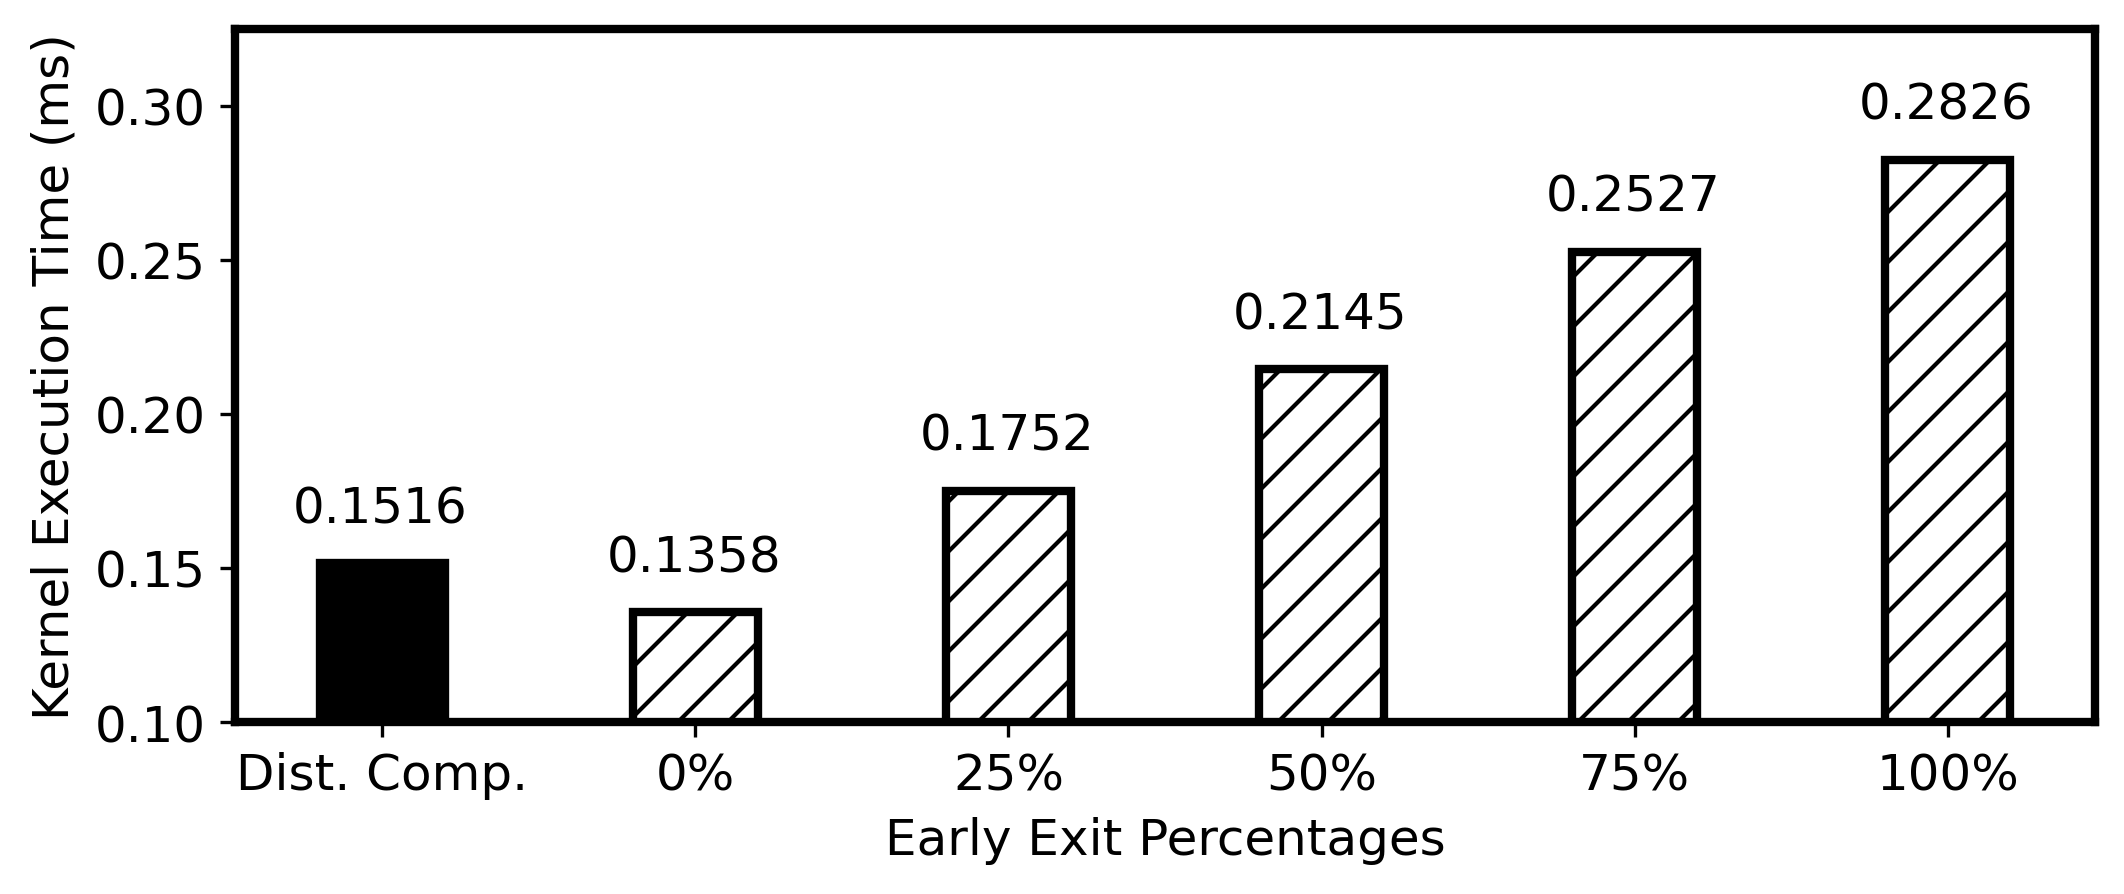
\includegraphics[scale=0.6]{figures/early_exit.png}}
    \caption{The \textit{k}-selection results with different early exit percentages}
    \label{fig:early_exit}
    \end{figure}

\begin{figure}[htbp]
    \begin{adjustbox}{addcode={
        \begin{minipage}{\width}}{
            \caption{The accelerations of the overall best best tiling shapes (MM + kSel) compared with the individual best tiling shapes (MM \& kSel)}
            \label{fig:final}
        \end{minipage}},rotate=90,center}
        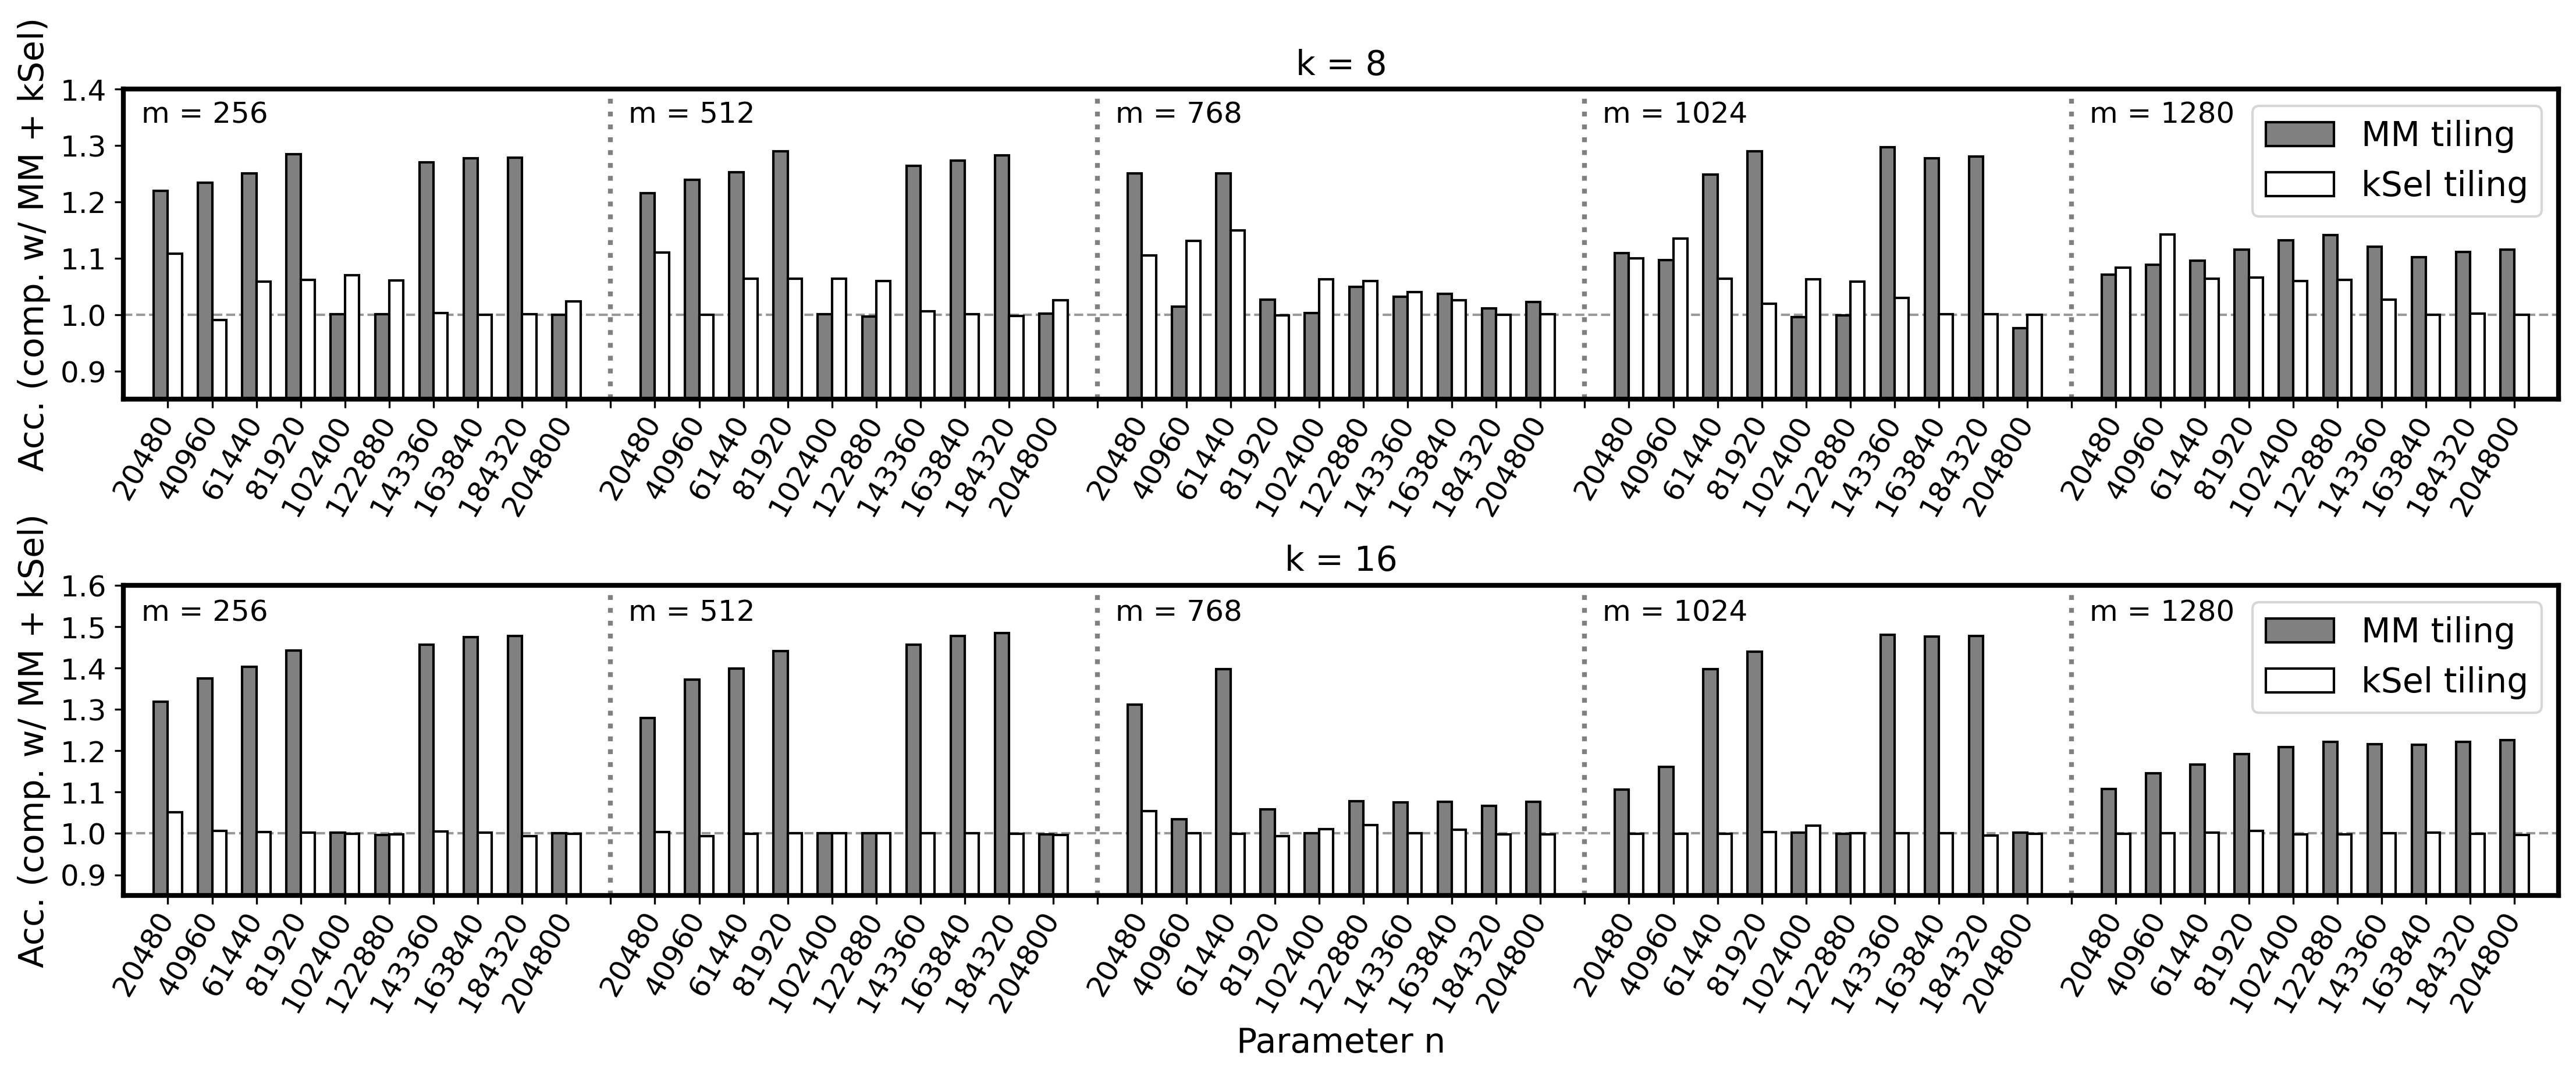
\includegraphics[scale=0.5]{figures/final_data.png}
    \end{adjustbox}
\end{figure}

By modifying the input datasets and the initial \textit{k}-min values, the number of updating values can be controlled intentionally. Therefore, we practically control and evaluate the execution time reduced by the early exit policy. Fig. \ref{fig:early_exit} illustrates the execution results for the case when $k = 16$ with the size of test dataset $(32 \times 128)$ and training dataset $(128 \times 4096)$. The early exit percentage represents the percentages of the workloads that have been done when the algorithm exits. We also add the execution time of the distance computation kernel to compute the exact proportion of the whole algorithm execution time being reduced.

The results report a linear growth of the \textit{k}-selection algorithm with the increment of the workloads. The \textit{k}-selection execution time of the case with all workloads is 2.08$\times$ than that with no workloads. For the whole algorithm execution time with the distance computation, the acceleration is 1.51$\times$. The results show that our early exit policy works well and significantly reduces the workload. In addition, even though there is no computation workload assigned to the kernel, the \textit{k}-selection algorithm still takes 0.1516 ms. The results show that the simple but slow scalar conditional branch operations take 48.22\% of the \textit{k}-selection kernel, which further shows the low performance of the scalar units on the AI processors.

\subsection{Mini-batch Execution of SelB-\textit{k}-NN}

\subsubsection{\textit{K}-selection Workload Quantification}

\begin{figure}[tbp]
    \centering{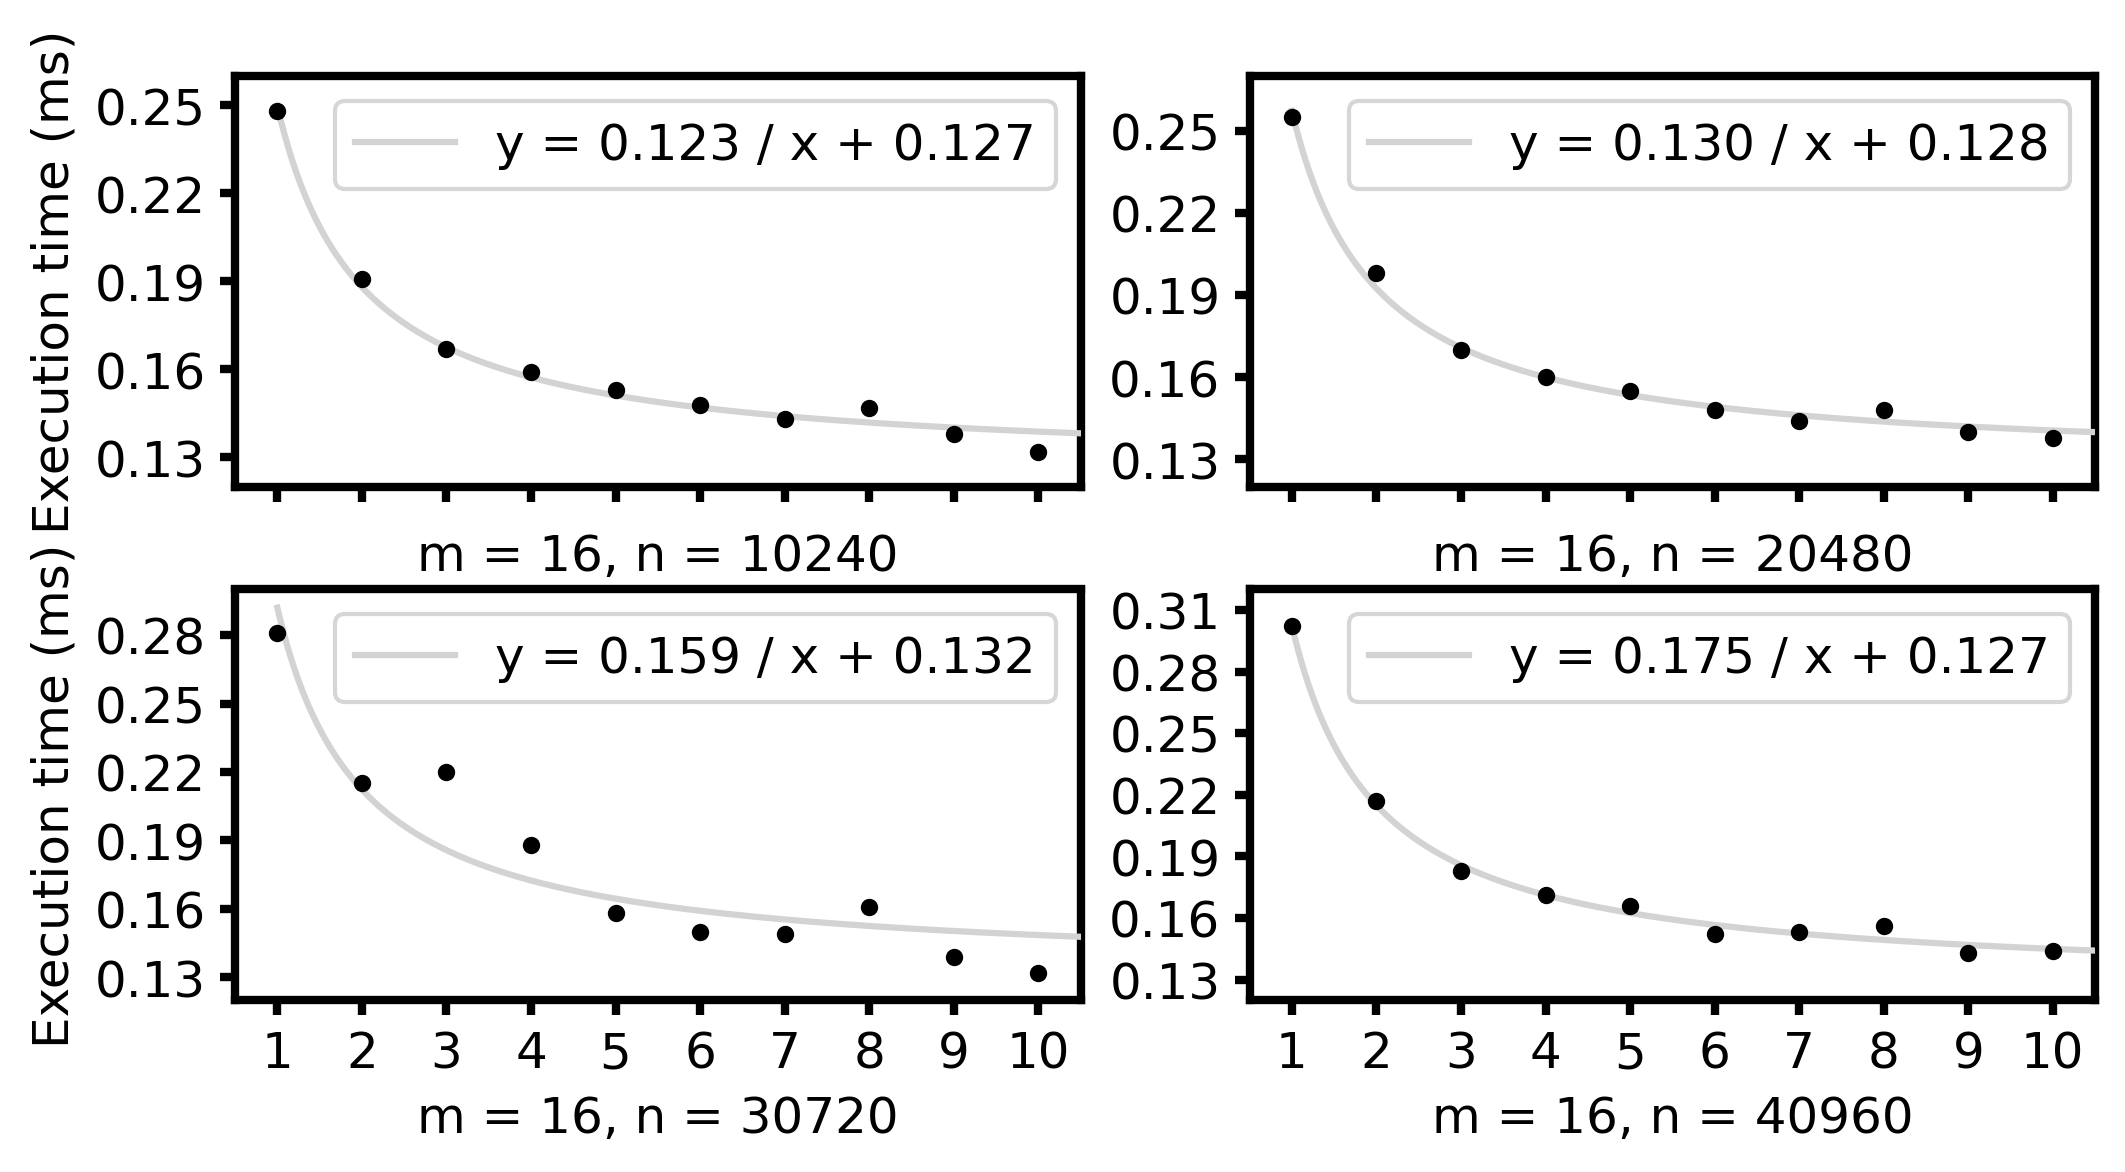
\includegraphics[scale=0.62]{figures/verified.png}}
    \caption{The \textit{k}-selection execution time of each tile and the fitting curves}
    \label{fig:verified}
    \end{figure}

We evaluate the execution time of sequential $k$-selection tiles after tiling, where each tile receives the min-$k$ results from the last adjacent tile to reduce its workloads. Fig. \ref{fig:verified} shows the evaluation results for four examples. The entire training dataset is divided into ten tiles along the $n$-direction. Each point in the figures represents the $k$-selection execution time of the \textit{t}-th tile.

For all four examples, the execution time decreases in an inverse proportion, as discussed in Sec. \ref{kSel}. The curves in the figures are fitted by the non-linear least squares method with an average coefficient of determination, $R^{2} = 0.97$. With the increment of $n$, the execution time of each \textit{t}-th tile increases plus a fixed constant cost of about 0.13 ms. For the example of $m = 16, n = 40960$, a tile is the single execution we shown in Sec. \ref{early}. Compared with the early exit results in Fig. \ref{fig:early_exit}, the workload being executed on each tile is apparent to be looked up, which also follows the inverse proportion. The curves and the workload variations evidence the correctness of our $k$-selection qualification.

\subsubsection{Mini-batch SelB-\textit{k}-NN Performance}

\begin{figure}[tbp]
    \centering{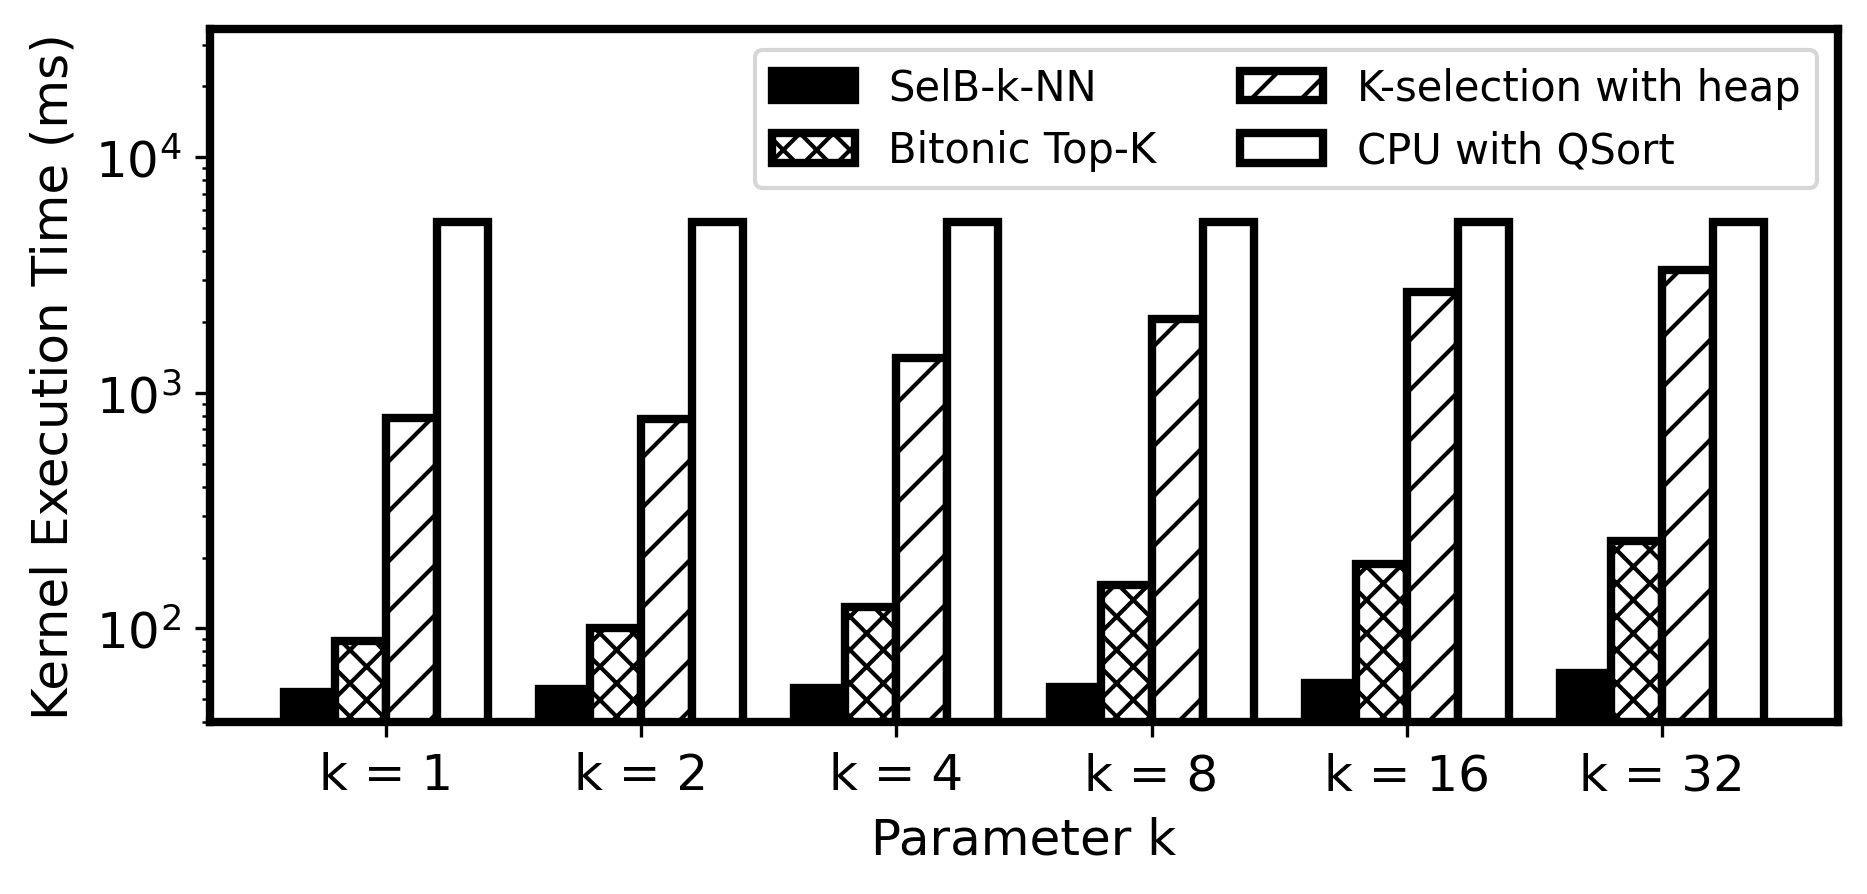
\includegraphics[scale=0.62]{figures/multi_results.png}}
    \caption{The \textit{k}-selection execution time of each tile and the fitting curves}
    \label{fig:multi_results}
    \end{figure}

We compare the performance of mini-batch SelB-\textit{k}-NN with other approaches with a larger dataset, where the test dataset is $(1280 \times 128)$ and the training dataset is $(128 \times 204800)$. The tiling shape we choose for SelB-\textit{k}-NN is $(16 \times 128)$ and $(128 \times 4096)$. 

Fig. \ref{fig:multi_results} shows the results for the comparison with different \textit{k}-values. Generally, compared with the single execution results, mini-batch SelB-\textit{k}-NN achieves higher accelerations. It reports an average speedup of 2.53$\times$ compared with the bitonic approaches, 31.24$\times$ with the heap approaches, and 92.75$\times$ with the CPU quicksort implementations. Meanwhile, with the increment of the \textit{k}-value, we observe the accelerations of SelB-\textit{k}-NN compared with other algorithms also grow significantly. The main reason for the higher accelerations is the early exit policy in SelB-\textit{k}-NN, which skipped most of the mini-batches in the large training dataset. 

\subsubsection{Tiling Shapes Results}

We evaluate the performance of SelB-\textit{k}-NN with different tiling shapes. We first profile the execution time of the matrix multiplication, $f(m_1, n_1)$, and that of the $k$-selection, $g(m_2, n_2)$ and $g_{0}(m_2, n_2)$. Then with the collected performance data, we solve the optimization problem in Eq. \ref{eq:optimized} for the optimal tiling shape $(m_1, n_1, m_2, n_2)$. In addition, we also solve the individual optimization problem of the matrix multiplication $(m_1, n_1)$ and \textit{k}-selection $(m_2, n_2)$ to apply them to the both phases for comparisons.

Fig. \ref{fig:final} illustrates the acceleration rates of the optimal tiling shapes (MM + kSel) compared with the other two tiling shapes (MM \& kSel) for the cases $k = 8$ and $k = 16$. Since the execution time of the CANN native matrix multiplication does not increase linearly with the expansion of the tiling shapes, the acceleration rates vary irregularly. Compared with the matrix multiplication tiling shapes, the optimal tiling shapes achieve an acceleration of 1.29$\times$ when $k = 8$ and 1.48$\times$ when $k = 16$. The acceleration is 1.14$\times$ when $k = 8$ and 1.05$\times$ when $k = 16$ compared with the \textit{k}-selection tiling shapes. The figure shows that the matrix multiplication tiling shapes significantly lower the performance in most cases. In contrast, the performance with the \textit{k}-selection tiling shapes is closer to that with the optimal tiling shapes. Moreover, the optimal tiling shape acceleration compared with the best matrix multiplication tiling shapes when $k = 16$ is larger than $k = 8$. The results are opposite for the acceleration compared with the best \textit{k}-selection tiling shapes. It is because when $k = 16$, the matrix multiplication occupies more proportions of the algorithm execution time. The whole execution is mainly determined by the \textit{k}-selection phase, which performs poorly with the matrix multiplication tiling shapes. Although the matrix multiplication also has a performance loss with the \textit{k}-selection tiling shapes, the execution time increment is far less than the decrement by the $k$-selection phase. For the case when $k = 8$, the reasons are symmetric. On the other hand, in some cases, the two tiling shapes both cause a worse performance than the performance with overall tiling shapes, where two phases have similar influences on the whole execution time.

In addition, with our pruning method, for the case when $k = 8$, 72.80\% of the optimization problem's search space is reduced; for $k = 16$, 55.23\% of the space is reduced. The percentage of the pruned domain is related to parameter $k$, which determines the proportion of the constant cost to the execution time related to the workloads of the $k$-selection.

\section{Conclusion \& Future Work}

This paper introduced SelB-\textit{k}-NN, which is a novel \textit{k}-NN algorithm specifically designed for the AI processors. Based on the fact that the scalar operations, vectorized comparisons \& selections perform unexpectedly poorly on the AI processors, the main idea of SelB-\textit{k}-NN is to decrease the two operations as much as possible combining the selection sort and bitonic $k$-selection. Since the AI processors produced by different manufacturers have various designs, we propose two algorithms to reduce hardware support requirements to the most critical operations of deep learning. Especially, the involvement of \verb|ReLU| in the bitwise operations brings new thoughts for the famous Bit Twiddling Hack problems. We believe our first step of this algorithm could inspire more brilliant ideas for those classical solutions when applied to the AI processors. For large datasets, we set up an optimization problem for the optimal performance based on accurate quantification with a pruning method working in the preprocessing stage.

In the future work, we plan to extend SelB-\textit{k}-NN to the popular variants of \textit{k}-NN, like \text{K}-Nearest Neighbor Graph (\text{k}-NNG). We are also attractive in exploring the programmability of \verb|ReLU| in more bitwise applications.


%=============================================================================

\chapter{Cube-f(x): Transforming to Matrix Multiplications}
\label{sec_4}

\section{Background \& Motivation \label{sec:2}}

Taylor series is a powerful mathematics tool to evaluate a special function by representing infinitely differentiable functions as series that only contain additions and multiplication. Eq. \ref{eq:taylor} shows the definition of the Taylor series. The polynomial part of the Taylor series is called the Taylor polynomial. In the interval of convergence, by increasing the order number $n$, the Taylor polynomial can approximate the original functions with ignorable errors.

\begin{equation}
    \label{eq:taylor}
    \begin{aligned}
    f(x) = \sum_{k = 0}^{n}\frac{f^{(k)}(a)}{k!}(x - a)^k + o[(x - a) ^ n]
    \end{aligned}
    \end{equation}

One of the most common approaches to compute a polynomial, including the Taylor polynomial, is Horner's Method. Computing an original form of $n$-degree polynomial, e.g., $p(x)$ in Eq. \ref{eq:horner}, requires $(n^2 + n)/2$ multiplications and $n$ additions. Horner's Method converts a $n$-degree polynomial to a combination of $n$ linear polynomials, which needs $n$ multiplications and additions only.

\begin{equation}
    \label{eq:horner}
    \begin{aligned}
    p(x) &= a_n x^n + a_{n - 1}x^{n - 1} + ... + a_1 x + a_0 \\
         &= (((a_n x + a_{n - 1}) x + a_{n - 2})x + ... + a_1) x + a_0 \\
    q(x) &= b_n x^n + b_{n - 1}x^{n - 1} + ... + b_1 x + b_0 \\
         &= (((b_n x + b_{n - 1}) x + b_{n - 2})x + ... + b_1) x + b_0
    \end{aligned}
    \end{equation}

Since on most platforms \cite{XILINX, X86, CUDA}, $n$ multiplications are still costly in hardware resources and time, researchers introduce CORDIC, aiming to avoid the multiplications of the Taylor polynomials. CORDIC is based on the idea of rotating a vector by an arbitrary angle, using a series of elementary rotations with predetermined angles. Fig. \ref{fig:cordic} shows how CORDIC rotates and the predetermined degrees $\theta$. Since $tan(\theta_i) = 2^{-i}$, the multiplications of the pseudo rotation formula in Eq. \ref{eq:cordic}, $y_itan\theta$ and $x_itan\theta$, can be replaced by right shifts.

\begin{figure}[tbp]
    \centering{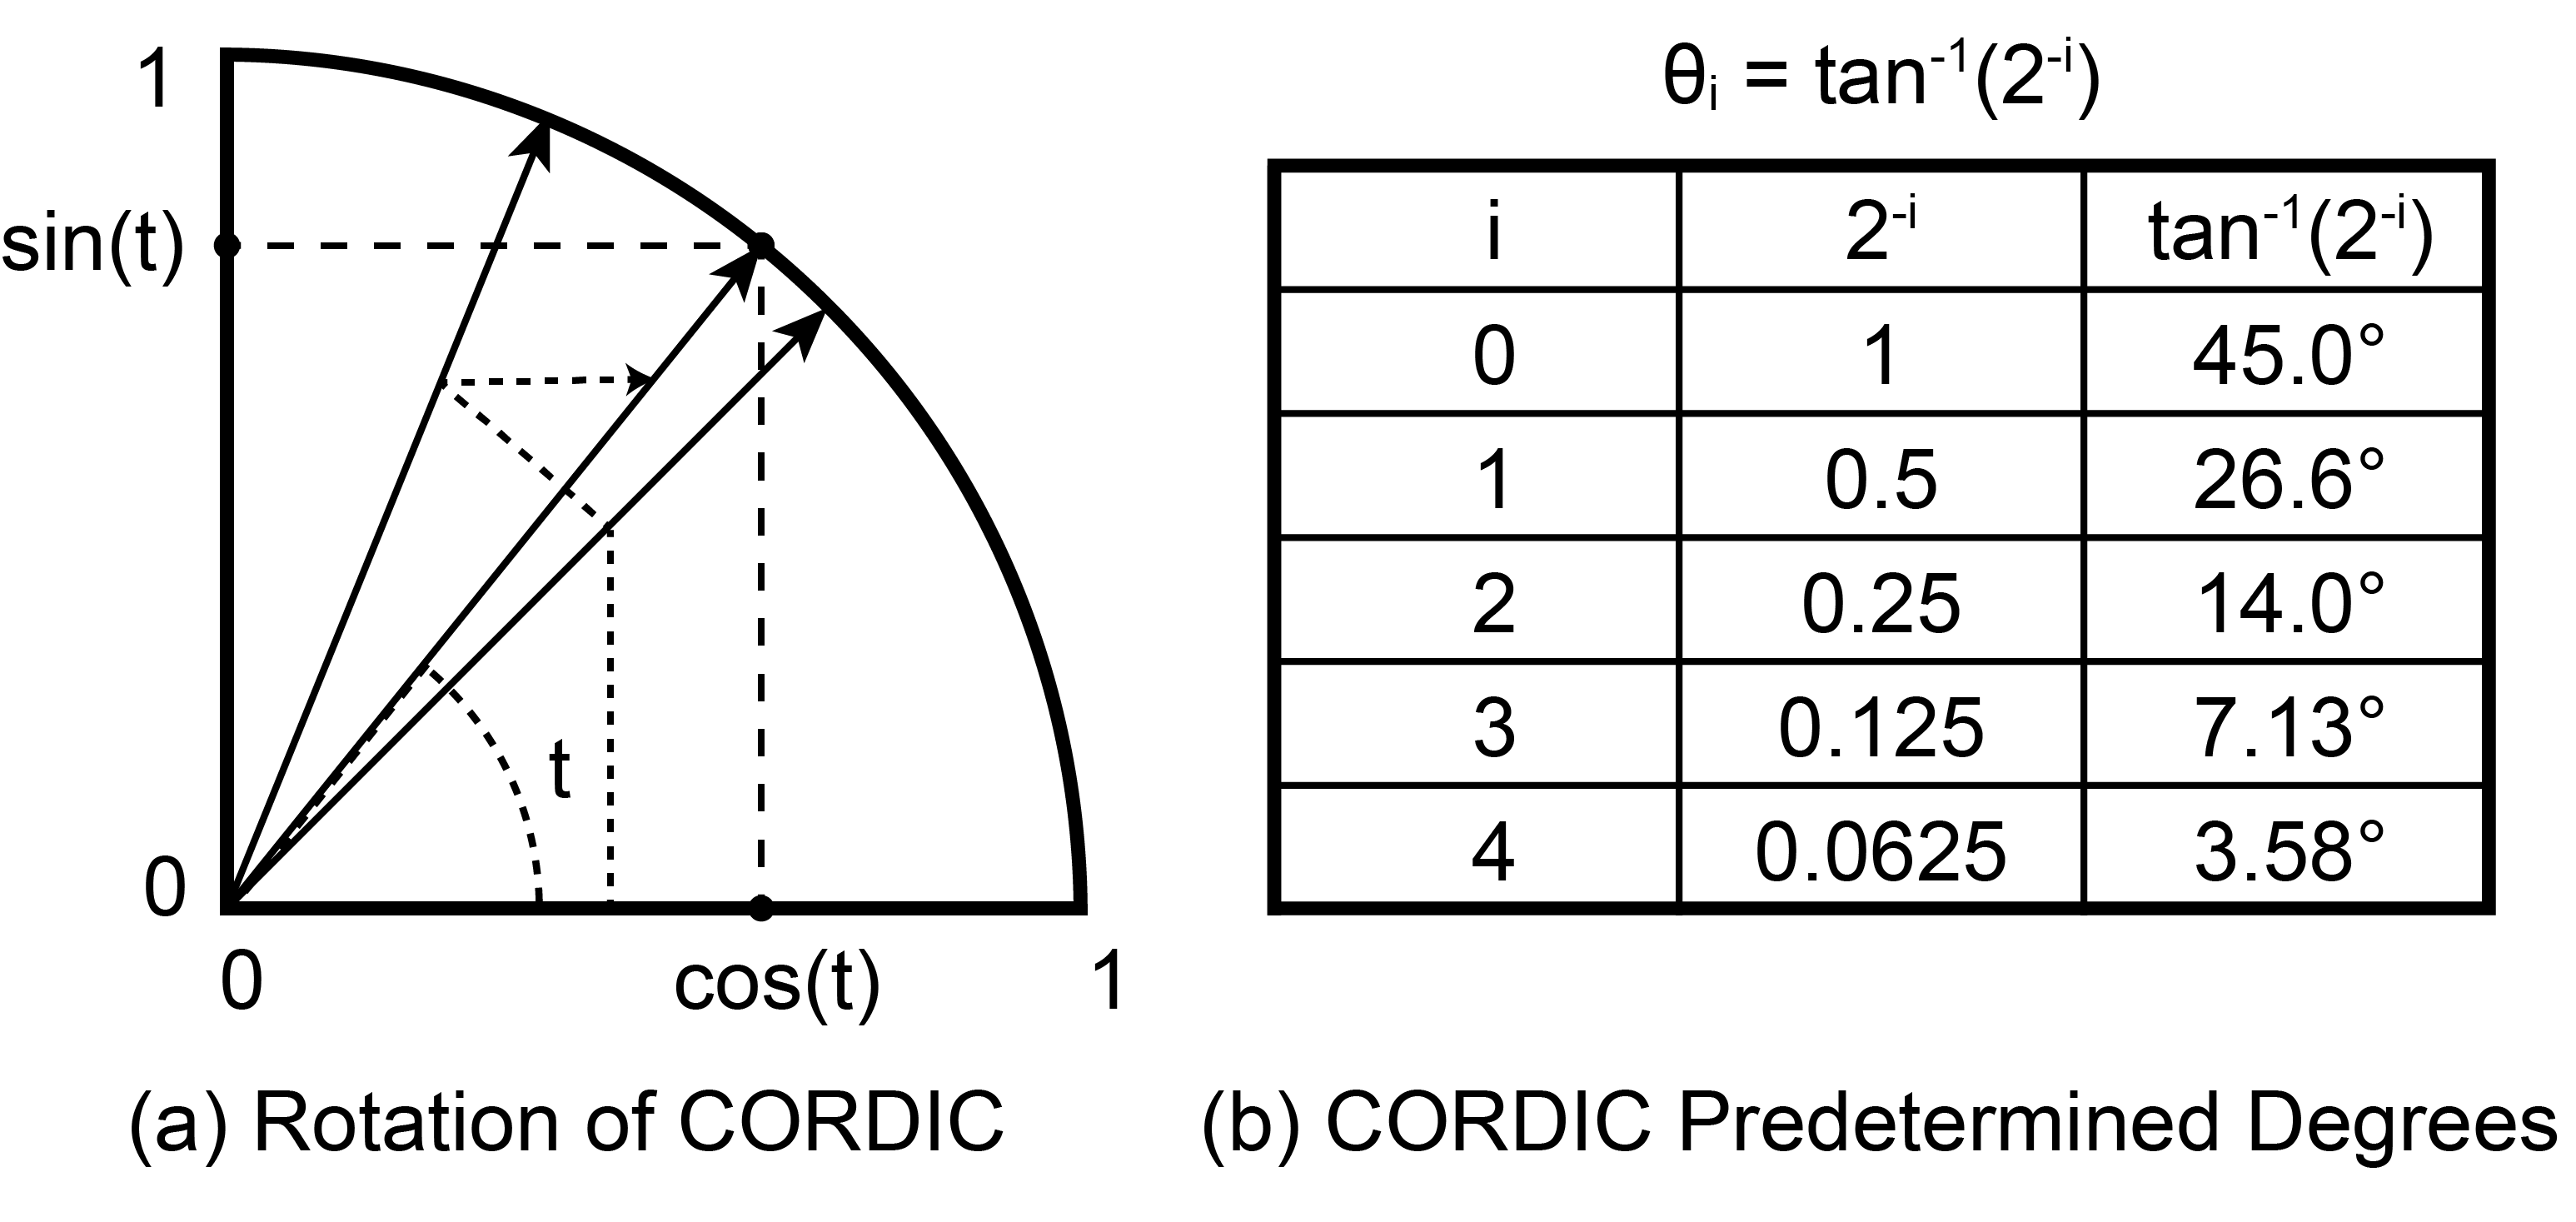
\includegraphics[scale=0.45]{figures/cordic.png}}
    \caption{CORDIC and the predetermined degrees}
    \label{fig:cordic}
    \end{figure}

\begin{equation}
    \label{eq:cordic}
    \begin{aligned}
    \left\{ 
        \begin{array}{lc}
            x_{i+1} = x_i - y_i tan\theta = x_i - y_i 2 ^ {-i} \\
            y_{i+1} = y_i + x_i tan\theta = y_i - x_i 2 ^ {-i}
        \end{array}
    \right.
    \end{aligned}
    \end{equation}

Nevertheless, as discussed in Sec. \ref{sec_1_2_2}, current AI processors lack or perform poorly on the shift operations, which makes CORDIC fail to mitigate the heavy performance loss caused by the weak vector units. 

In addition, in some AI or scientific applications, e.g., the combination of multiple activations \cite{DBLP:conf/icpr/ManessiR18} or loss functions \cite{DBLP:conf/cvpr/KendallGC18}, the computation of Euler angles from rotation matrices \cite{weissteinrotation}, a piece of data needs to be computed by multiple independent functions. In these situations, both previous methods must repeat the same process. Especially for the Taylor polynomials with Horner's Method, although the two functions, e.g., $p(x)$ and $q(x)$ in Eq. \ref{eq:horner}, share the same variable $x$ and computation process, their computations are independent. The intermediate result $(a_nx + a_{n-1})$ of $p(x)$ is discarded immediately after the computation of $p(x)$ and cannot be reused by $q(x)$. On the other hand, for the original form of Taylor polynomials without using Horner's Method, the variable sequence $(x^n, x^{n-1}, ..., x)$ can serve as a common intermediate result. If the computation of $p(x)$ had generated the variable sequence, $q(x)$ could reuse it for its subsequent computation. For multiple functions to be computed, all could reuse the variable sequence, whereas Horner's Method must compute from the beginning. However, the building of the variable sequence $(x^n, x^{n-1}, ..., x)$ is expected to be time-consuming. Even if the variable sequence is available, the remaining computation to complete the polynomials requires the same number of operations as Horner's Method. Therefore, exploiting potential data reuse for multiple function evaluations is difficult.

\section{Cube-f(x) Algorithm \label{sec:3}}

Fig. \ref{fig:overview} gives an overview of Cube-$f(x)$. It contains two main stages: the preparation stage and the computation stage. In the preparation stage, Cube-$f(x)$ uses a series of specifically designed Sequence Matrices to generate Variable Sequence $(x, x^2, x^3, ...)$ with input $x$. In the computation stage, Cube-$f(x)$ accepts Coefficients Matrices, which contain multiple Taylor polynomial coefficients, with the Variable Sequence to evaluate the equivalent functions' values. While Fig. \ref{fig:overview} illustrates the computation of a single input for a more precise understanding, Cube-$f(x)$ always takes an array as inputs. Therefore, the Variable Sequence and the final computation results are 2D arrays containing the evaluation results of different functions for multiple inputs.

This section first introduces the computation stage, which is more straightforward, and then the preparation stage. This order helps us to understand the design tradeoff of the preparation stage, which is caused by the specific data layout requirement of the computation stage.

\begin{figure}[t]
    \centering{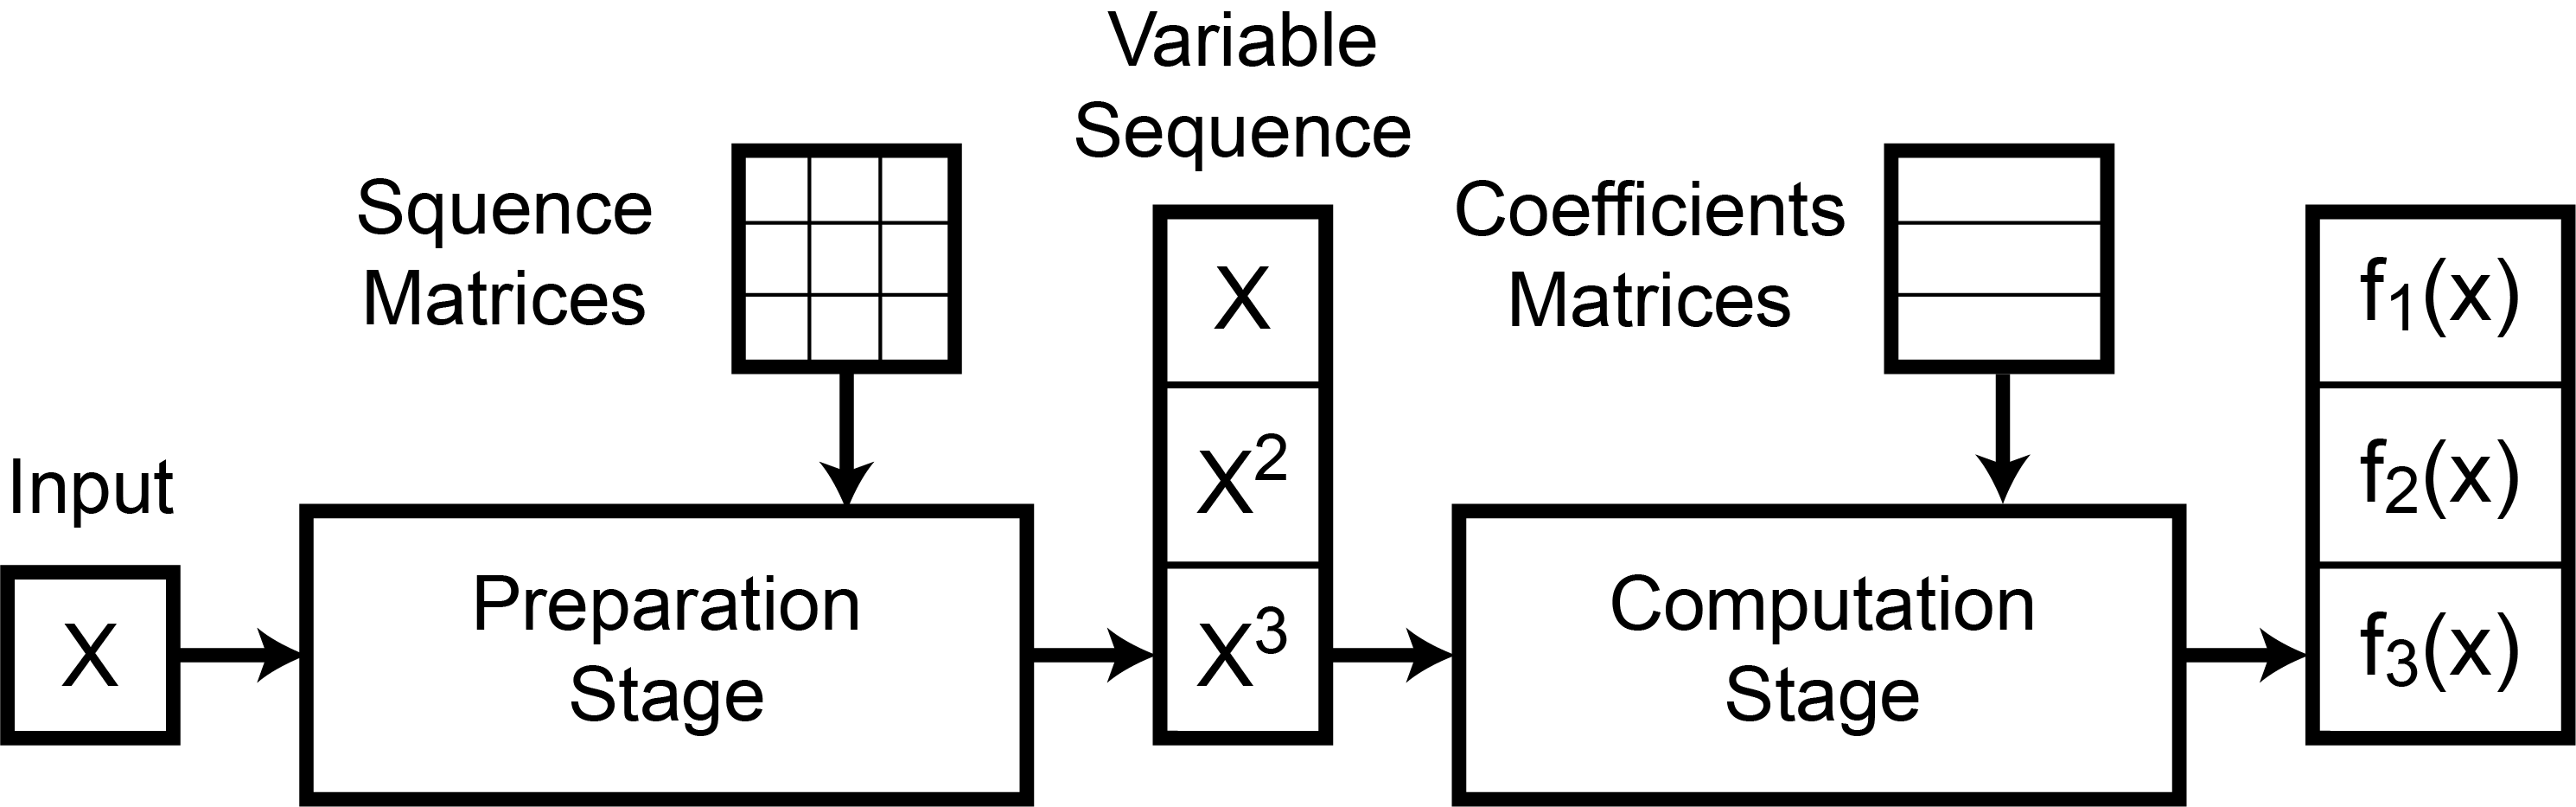
\includegraphics[scale=0.45]{figures/overview_2.png}}
    \caption{An overview of Cube-$f(x)$ Algorithm for a single input}
    \label{fig:overview}
    \end{figure}

\subsection{Computation Stage}

\begin{equation}
    \label{eq:comp_mat}
    \begin{aligned}
    \setlength{\arraycolsep}{1.5pt}
        \begin{bmatrix} 
            x_1    & x_1^2  &   \dots   & x_1^k  \\
            x_2    & x_2^2  &   \dots   & x_2^k  \\
            \vdots &        & \ddots    & \vdots \\
            x_m    & x_m^2  &   \dots   & x_m^k  
        \end{bmatrix}
        \begin{bmatrix} 
            a_1    & b_1    &   \dots   & j_1 \\
            a_2    & b_2    &   \dots   & j_2  \\
            \vdots &        & \ddots    & \vdots \\
            a_k    & b_k    &   \dots   & j_k  
        \end{bmatrix}
        \approx
        \begin{bmatrix}
            f_{a}(x_1)  &     \dots   & f_{j}(x_1)    \\
            f_{a}(x_2)  &     \dots   & f_{j}(x_2)    \\
            \vdots      & \ddots    & \vdots        \\
            f_{a}(x_m)  &   \dots   & f_{j}(x_m)
        \end{bmatrix} \\
        f_t(x) = \sum_{s = 0}^{k}\frac{f_t^{(s)}(a)}{s!}(x - a)^s + o[(x - a) ^ k] \\
        \approx t_1x + t_2x^2 + \dots + t_kx^k
    \end{aligned}
    \end{equation}

The computation stage is mainly a matrix multiplication, shown in Eq. \ref{eq:comp_mat}, where $m$ is the number of inputs, $k$ is the order number, and $j$ is the number of evaluated functions. The left matrix of the matrix multiplication is a matrix of the Variable Sequence $(x, x^2, x^3, ...)$, which is built from the inputs and listed in the row-major order. The right matrix is the Coefficients Matrix, which is expanded from multiple functions to $n$ order and listed in the column-major order. In this way, each element of the result matrix is a function evaluation result based on its related Taylor polynomial. As a result, the matrix multiplication evaluates $m \times k$ Taylor polynomials in one step with the powerful Matrix MACs of the AI processors. 

Since the evaluated functions are chosen before launching the kernel, the values of the right matrix, the Coefficient Matrix, are predetermined and constant. Therefore, we consider the Coefficient Matrix a read-only memory segment that can be directly written in kernel codes. On the other hand, the data layout requirement of the left matrix, the Variable Sequence Matrix, is more stringent. The Matrix MAC of the AI processors usually adopts the row-major order for the left matrix in the matrix multiplication to achieve high efficiency \cite{cambricon, CANN, jax}. It means a variable sequence $(x_{i}, x_{i}^2,  x_{i}^3, ...)$, mapped by the input $x_{i}$, should be stored contiguously in the memory. Therefore, after the preparation stage, the data at the memory address $x_{i + 1}$ in the kernel inputs should be moved to $x_{i + k}$ with its powers at $(x_{i + k + 1}, x_{i + k + 2}, ...)$ in the Variable Sequence Matrix. Without a built-in vectorized \textit{scatter} instruction, the scattering process could only be done by weak scalar operations for each input $x_{i}$, significantly ruining the kernel performance. Therefore, the primary objective of the preparation stage is to complete the scattering process with the Matrix MACs instead of the vector or scalar units.

\subsection{Preparation Stage}

The preparation stage of Cube-$f(x)$ is based on two mathematical formulas. The first combines the logarithmic power law and the logarithmic definition, given in Eq. \ref{eq:power}, which allows us to convert the product to power.

\begin{equation}
    \label{eq:power}
    \begin{aligned}
        e^{p \ln x} = e^{\ln x^p} = x^p
    \end{aligned}
    \end{equation}

The second formula is a particular case of matrix multiplications, given in Eq. \ref{eq:spec_mat}, where the left matrix is an input matrix of $m \times n$ and the right matrix $\textbf{B}$ is a matrix of $n \times j_0$. Except for a non-zero vector $(k_0, k_1, \dots, k_{j_0})$ at the row $i_0$, all other elements of $\textbf{B}$ are $0$. The matrix multiplication Eq. \ref{eq:spec_mat} first does a scattering process for a target column $i_0$ with a stride of $j_0$, then it duplicates the columns to fill the gaps. Finally, it computes the products of the columns and the related coefficients $(k_0, k_1, \dots, k_{j_0})$ to form a full matrix.

\begin{equation}
    \label{eq:spec_mat}
    \begin{aligned}
        \setlength{\arraycolsep}{2pt}
        \begin{bmatrix} 
            p_{1, 1}    & \dots     & p_{1, n}  \\
            \vdots      & \ddots    & \vdots    \\
            p_{m, 1}    & \dots     & p_{m, n} 
        \end{bmatrix}
        \cdot
        \textbf{B}
        =
        \begin{bmatrix}
            k_1 p_{1, i_0}  & \dots     & k_{j_0} p_{1, i_0}    \\
            \vdots          & \ddots    & \vdots                \\
            k_1 p_{m, i_0}  & \dots     & k_{j_0} p_{m, i_0}    \\
        \end{bmatrix} \\
        \textbf{B} = (b_{i, j}) \in \mathbb{F}^{n \times j_0}, 
        b_{i, j} = \left\{
                        \begin{array}{lc}
                            0, i \neq i_{0} \\
                            k_j, i = i_{0}
                        \end{array}
                    \right.
    \end{aligned}
    \end{equation}

\begin{algorithm}[tbp]
    \caption{Preparation Stage of Cube-$f(x)$}
    \setlength{\arraycolsep}{1.2pt}
    \label{alg:prepare}
    \SetKwInOut{Input}{Input}
    \SetKwInOut{Output}{Output}
        
    \Input{
        input 1D array \textbf{V} of the size $N$ \\
    }
    \Output{
        result sequences \textbf{Sq} of the size $N \times k$
    }
    
    \BlankLine
    \BlankLine
    
    $mat[s] \leftarrow 
            \begin{bmatrix} 1 & 2 & \dots & k   \\ 
                            &   &   \dots &     \\ 
                            0 & 0 & \dots & 0 
            \end{bmatrix}
            \dots
            \begin{bmatrix} &   &   \dots &     \\ 
                            1 & 2 & \dots & k   \\ 
                            &   &   \dots &     
            \end{bmatrix}
            \dots
            \begin{bmatrix} 0 & 0 & \dots & 0   \\
                            &   &   \dots &     \\ 
                            1 & 2 & \dots & k
            \end{bmatrix}
    $ \\
    \BlankLine
    \BlankLine
    $\textbf{V}_{ln} \leftarrow \textbf{ln}(\textbf{V})$ \\
    $\textbf{V}_{mat} \leftarrow$ reinterpret $\textbf{V}_{ln}$ as a $(N / s) \times s$ matrix \\
    \For{$idx \leftarrow 0$ \KwTo $s$} {
        $\textbf{Sq}_{mat}[idx] \leftarrow \textbf{V}_{mat} \cdot mat[idx]$ \\
        $\textbf{Sq}_{ln}[idx] \leftarrow$ reinterpret $\textbf{Sq}_{mat}[idx]$ as an 1D array \\
        $\textbf{Sq}[idx] \leftarrow $ \textbf{exp}($\textbf{Sq}_{ln}[idx]$)
    }
    \Return \textbf{Sq}
\end{algorithm}

Based on the two formulas, Alg. \ref{alg:prepare} presents the preparation stage of Cube-$f(x)$, where we consider the shape of the Matrix MACs is $(s \times s)$.

In the beginning, Alg. \ref{alg:prepare} initializes an array of $(s \times k)$ Sequence Matrices $mat[s]$, which we described as $\textbf{B}$ in Eq. \ref{eq:spec_mat}. For the $idx$-th Sequence Matrix $mat[idx]$, the non-zero row is at row $idx$, whose value is an increasing vector $(1, 2, \dots, k)$. Therefore, for each row $idx$ of the $(s \times s)$ Matrix MACs, we construct a unique Sequence Matrix with a non-zero vector at that row. Then, Alg. \ref{alg:prepare} computes the logarithmic results $\textbf{V}_{ln}$ of the input $\textbf{V}$ with the built-in vectorized operation. The logarithmic results are reinterpreted as an $(\frac{N}{s} \times s)$ matrix $\textbf{V}_{mat}$ and directly transferred to the matrix MAC. Especially, the reinterpretation needs no physical data layout conversion but only from the logical view. 

\begin{figure}[t]
    \centering{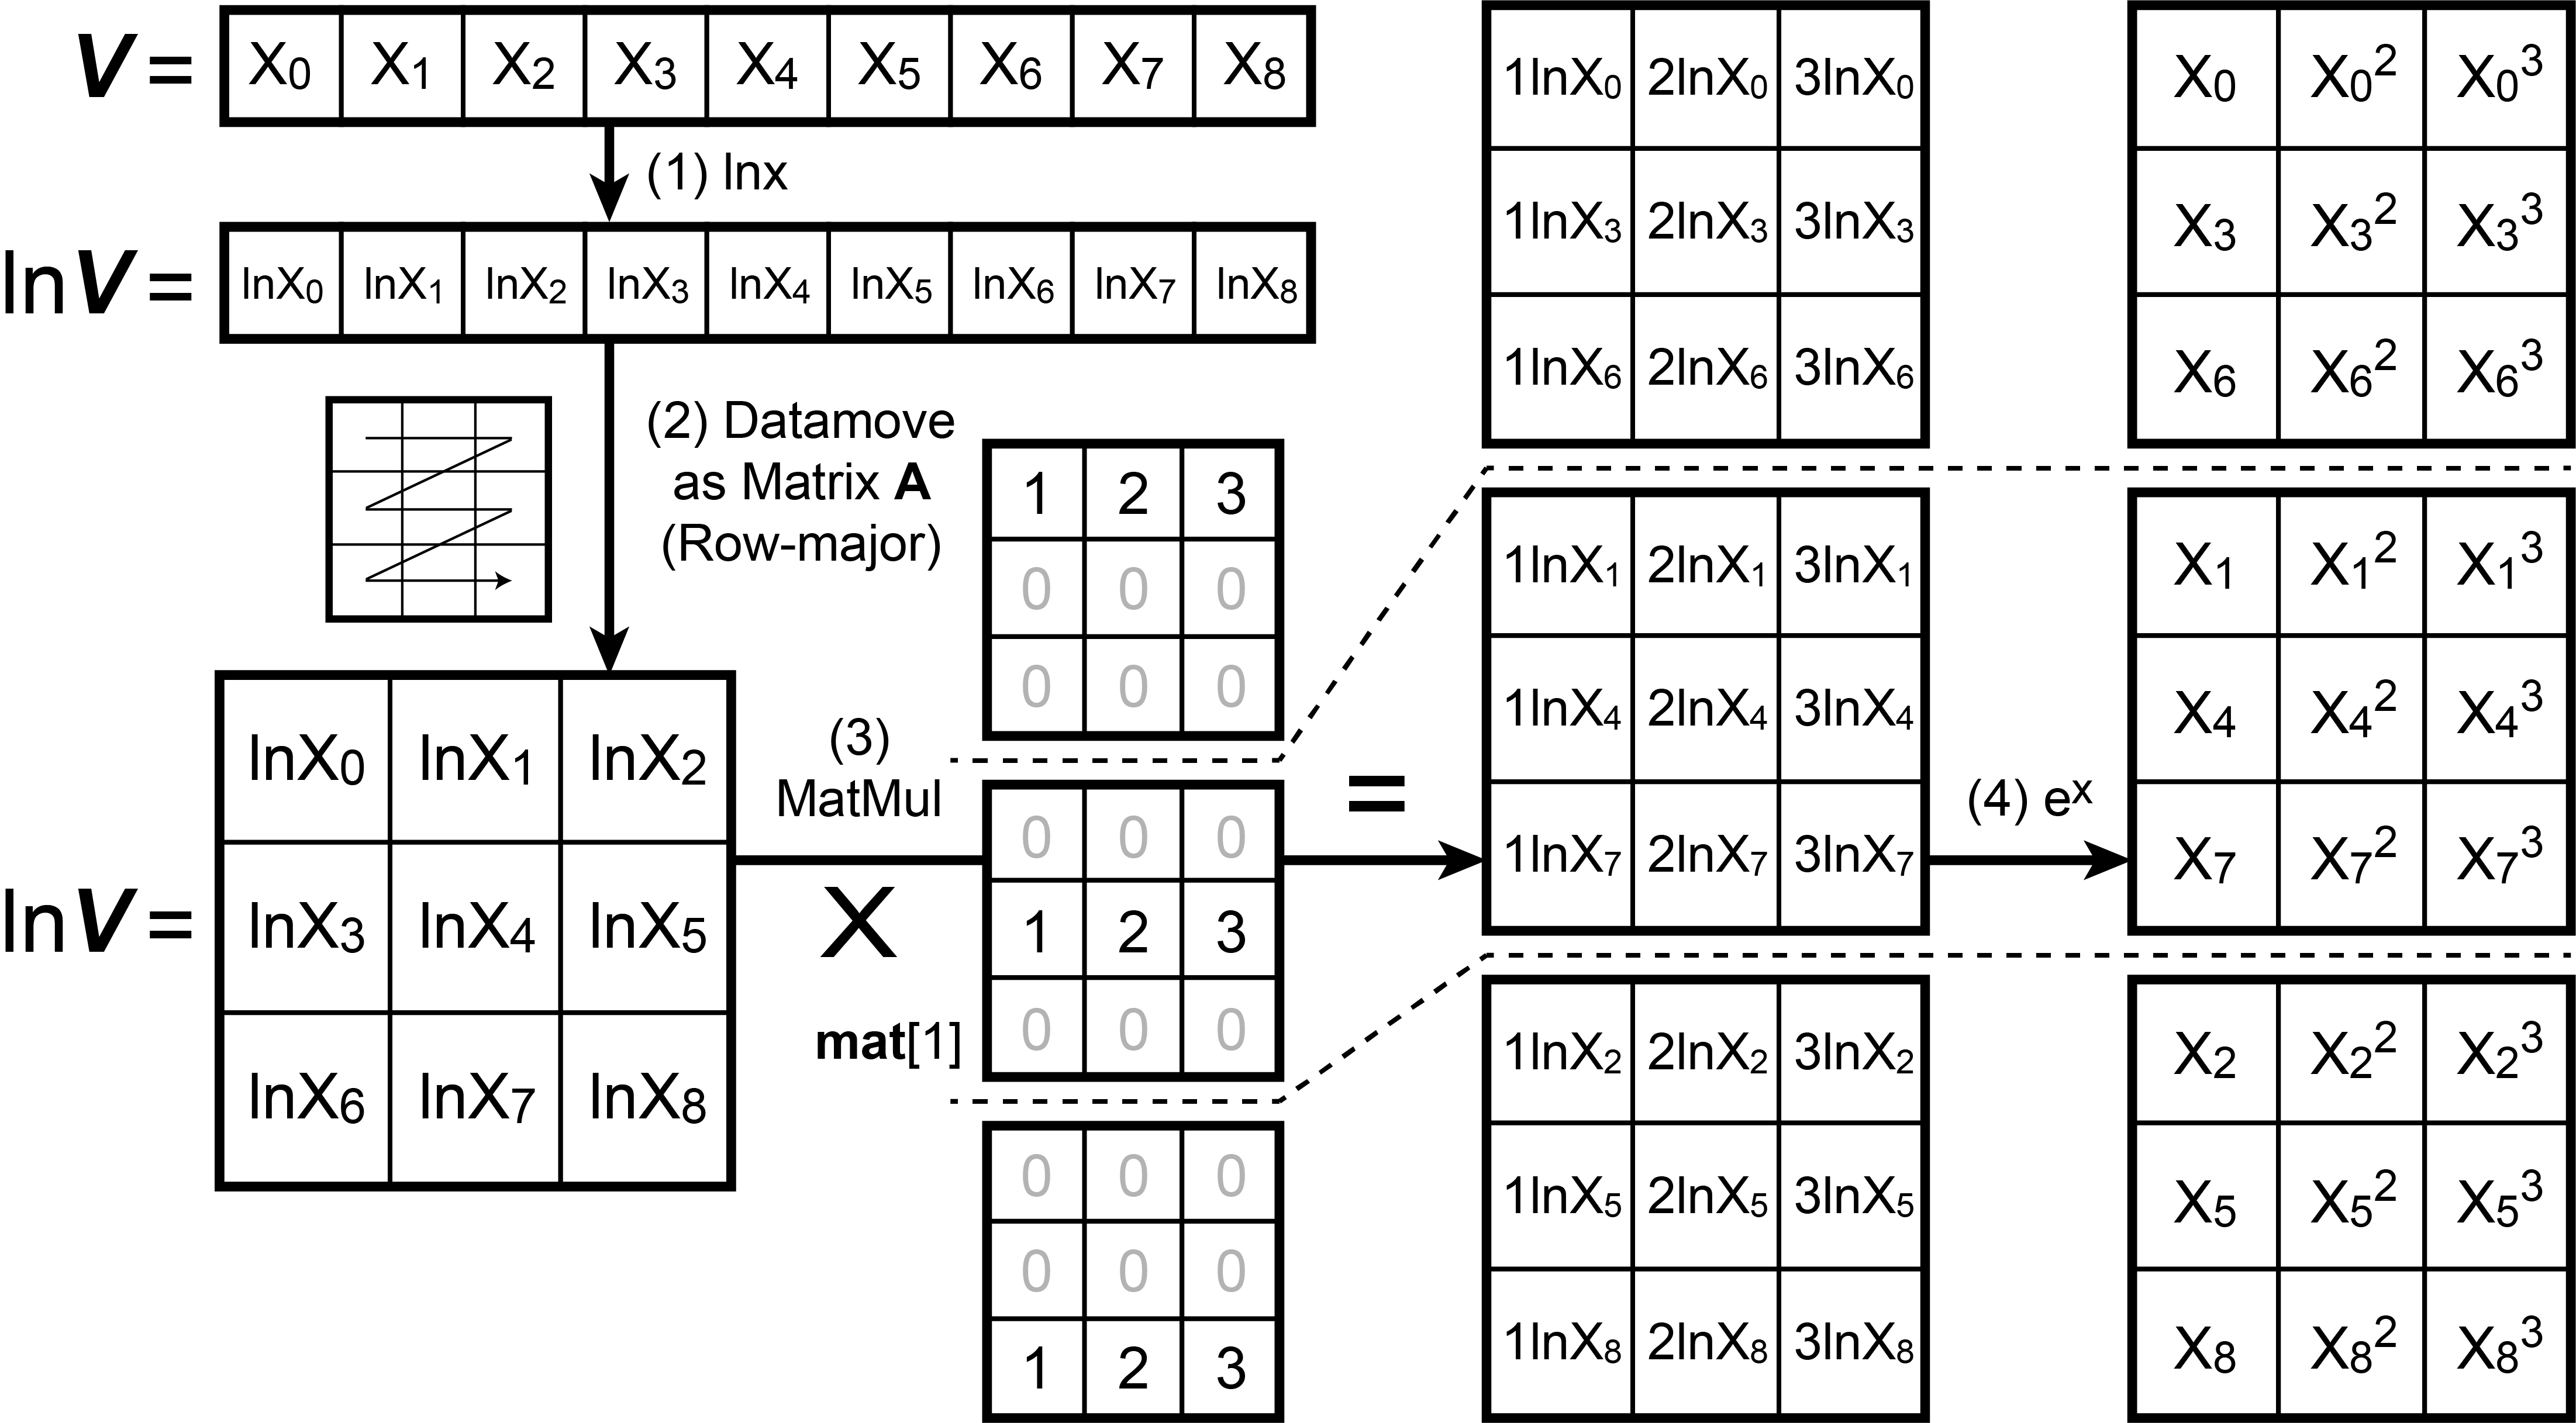
\includegraphics[scale=0.32]{figures/trans_ln.png}}
    \caption{An example for 9 inputs with $3 \times 3$ Matrix MACs}
    \label{fig:trans_ln}
    \end{figure}

The next step is the central step of the preparation stage, which is an $s$-step loop. In the loop step $idx$, the logarithmic inputs $\textbf{V}_{mat}$ take matrix multiplications with the Sequence Matrix $mat[idx]$. As discussed in Eq. \ref{eq:spec_mat}, the $idx$-th matrix multiplication generates the $(\frac{N}{s} \times n)$ Variable Sequence matrix for the column $idx$ of the logarithmic inputs. For the example of the second matrix multiplication in Fig. \ref{fig:trans_ln}, the non-zero row of the second Sequence Matrix $mat[1]$ is at the second row $mat[1][1, :]$. Therefore, the result matrix is formed by the product of the second column of the logarithmic inputs $\textbf{V}_{mat}[:, 1]$ and the increasing vector $(1, 2, \dots, k)$. Since the logarithmic results are shaped as $(\frac{N}{s} \times s)$, $s$ columns need $s$ loop steps and the Sequence Matrice in total.

After the matrix multiplication in each loop step, the preparation stage applies an exponential function to the result matrices, which is reinterpreted as an array. As shown in Eq. \ref{eq:power}, it restores the logarithmic product results $\textbf{Sq}_{ln}$ to the original power results. Finally, the preparation stage completes the construction of the Variable Sequence, which perfectly meets the data layout requirement of the computation stage. In addition, although the results are currently shaped as an array, similar to $\textbf{V}_{ln}$ without extra operations, they can be directly passed to the computation stage as $(\frac{N}{s} \times k)$ matrices.

The time complexity of the preparation stage is $O(Nk + Nk / s^2)$, where $N$ is the size of input data, $k$ is the order number of the Taylor expansion, and $s$ is the side length of the Matrix MACs. The first part $O(Nk)$ is the time complexity of the vectorized operations, which equals that of Horner's Method. The second part $O(Nk / s^2)$ is the time complexity of the matrix multiplications on the Matrix MACs. Theoretically, the execution time of the preparation stage is slightly longer than Horner's Method for a single-function evaluation. The slowdown here is acceptable since the preparation stage is built for multiple functions instead of only one function.

\begin{figure}[t]
    \centering{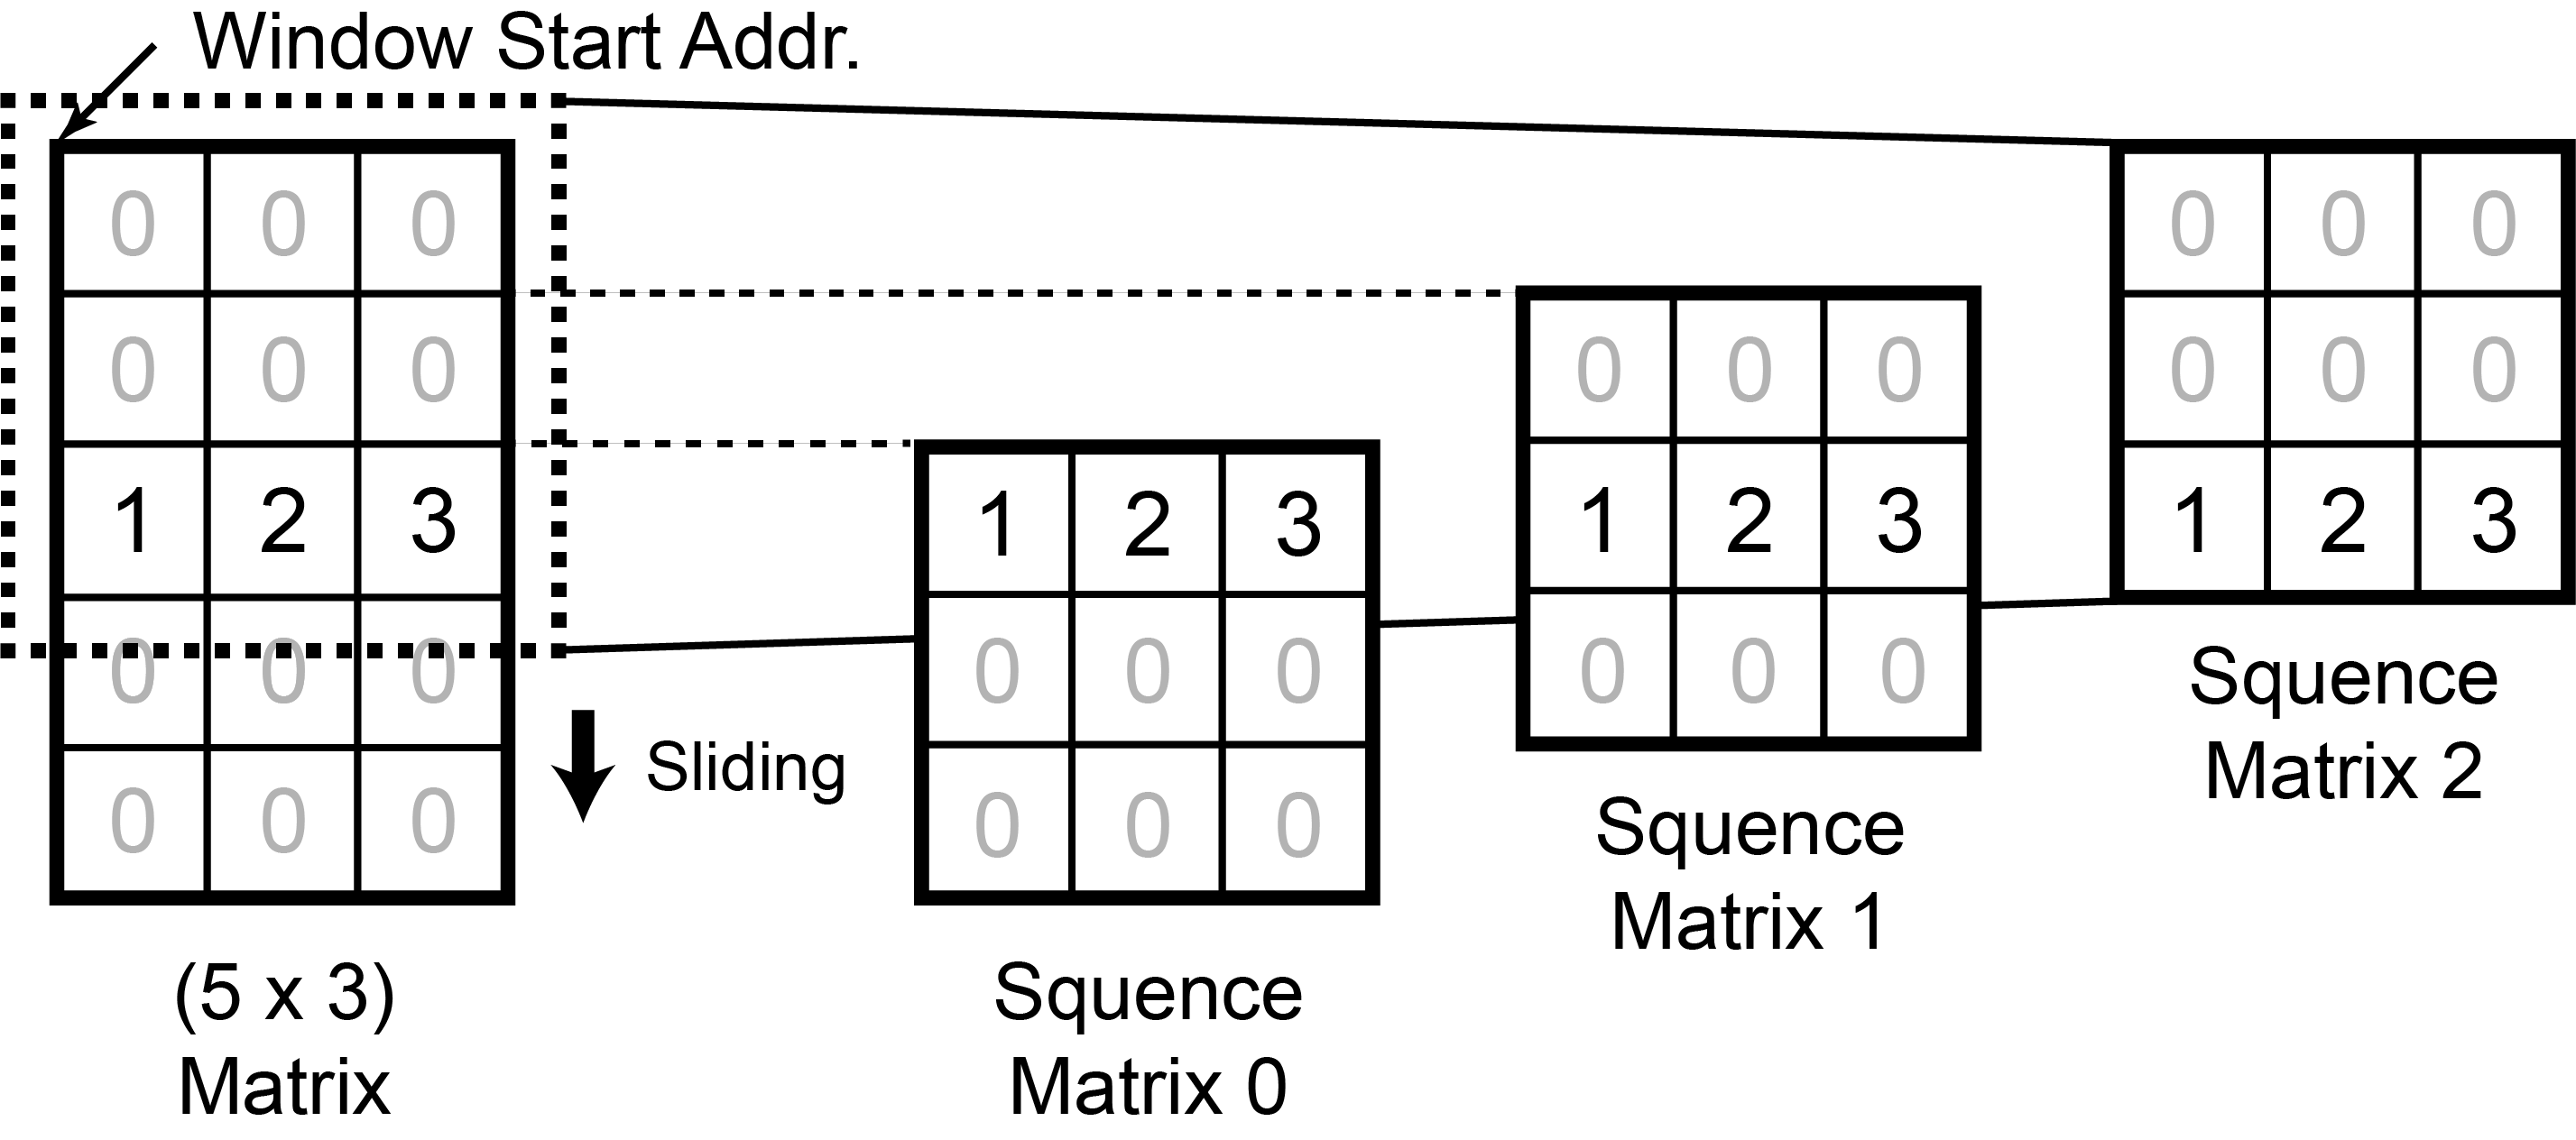
\includegraphics[scale=0.45]{figures/window.png}}
    \caption{An example for 9 inputs with $3 \times 3$ Matrix MACs}
    \label{fig:window}
    \end{figure}

For the space complexity, the extra memory needed by the preparation stage is $O(ks^2)$, which stores the preparation matrices. However, a sliding window policy can reduce the space complexity to $O(ks)$, which allocates $((2/s - 1) \times n)$ matrix. As shown in \ref{fig:window}, the non-vector is at the second row, while other rows are filled with $0$. Therefore, when the $(3 \times 3)$ windows slide down from row $0$ to row $2$, the three required Sequence Matrices are offered respectively.

\section{Cube-f(x) for General Cases \label{sec:4}}

The last section introduces Cube-$f(x)$ in the case where the Matrix MACs are always fully utilized. In this section, we extend the algorithm to more general instances where the Matrix MACs are not saturated ($k \mod s \neq 0$).

We first define a metric, Matrix MAC Count, to evaluate the scale of matrix multiplication. As mentioned in Sec. \ref{sec_1_2_2}, in one elementary step, a Matrix MAC completes a fixed shape of matrix multiplication. Then, it accumulates the results from multiple steps as a whole matrix multiplication by the law of block matrix multiplication. Therefore, the Matrix MAC Count indicates how many elementary fix-shaped matrix multiplications it takes for a Matrix MAC to finish a large matrix multiplication with the standard $O(n^3)$ block matrix multiplication algorithm. For example, for a Matrix MAC of the shape $(s \times s)$, the Matrix MAC Count of matrix multiplication of the shape $(m \times k \times n)$ is $(mkn / s^3)$.

Since the other operations, including data transfers and vectorized operations, roughly grow linearly with the number of matrix multiplications in Cube-$f(x)$, we directly use the Matrix MAC Count to compare the execution time in this section for simplicity.

\subsection{In-matrix Parallelism}

\begin{figure}[t]
    \centering{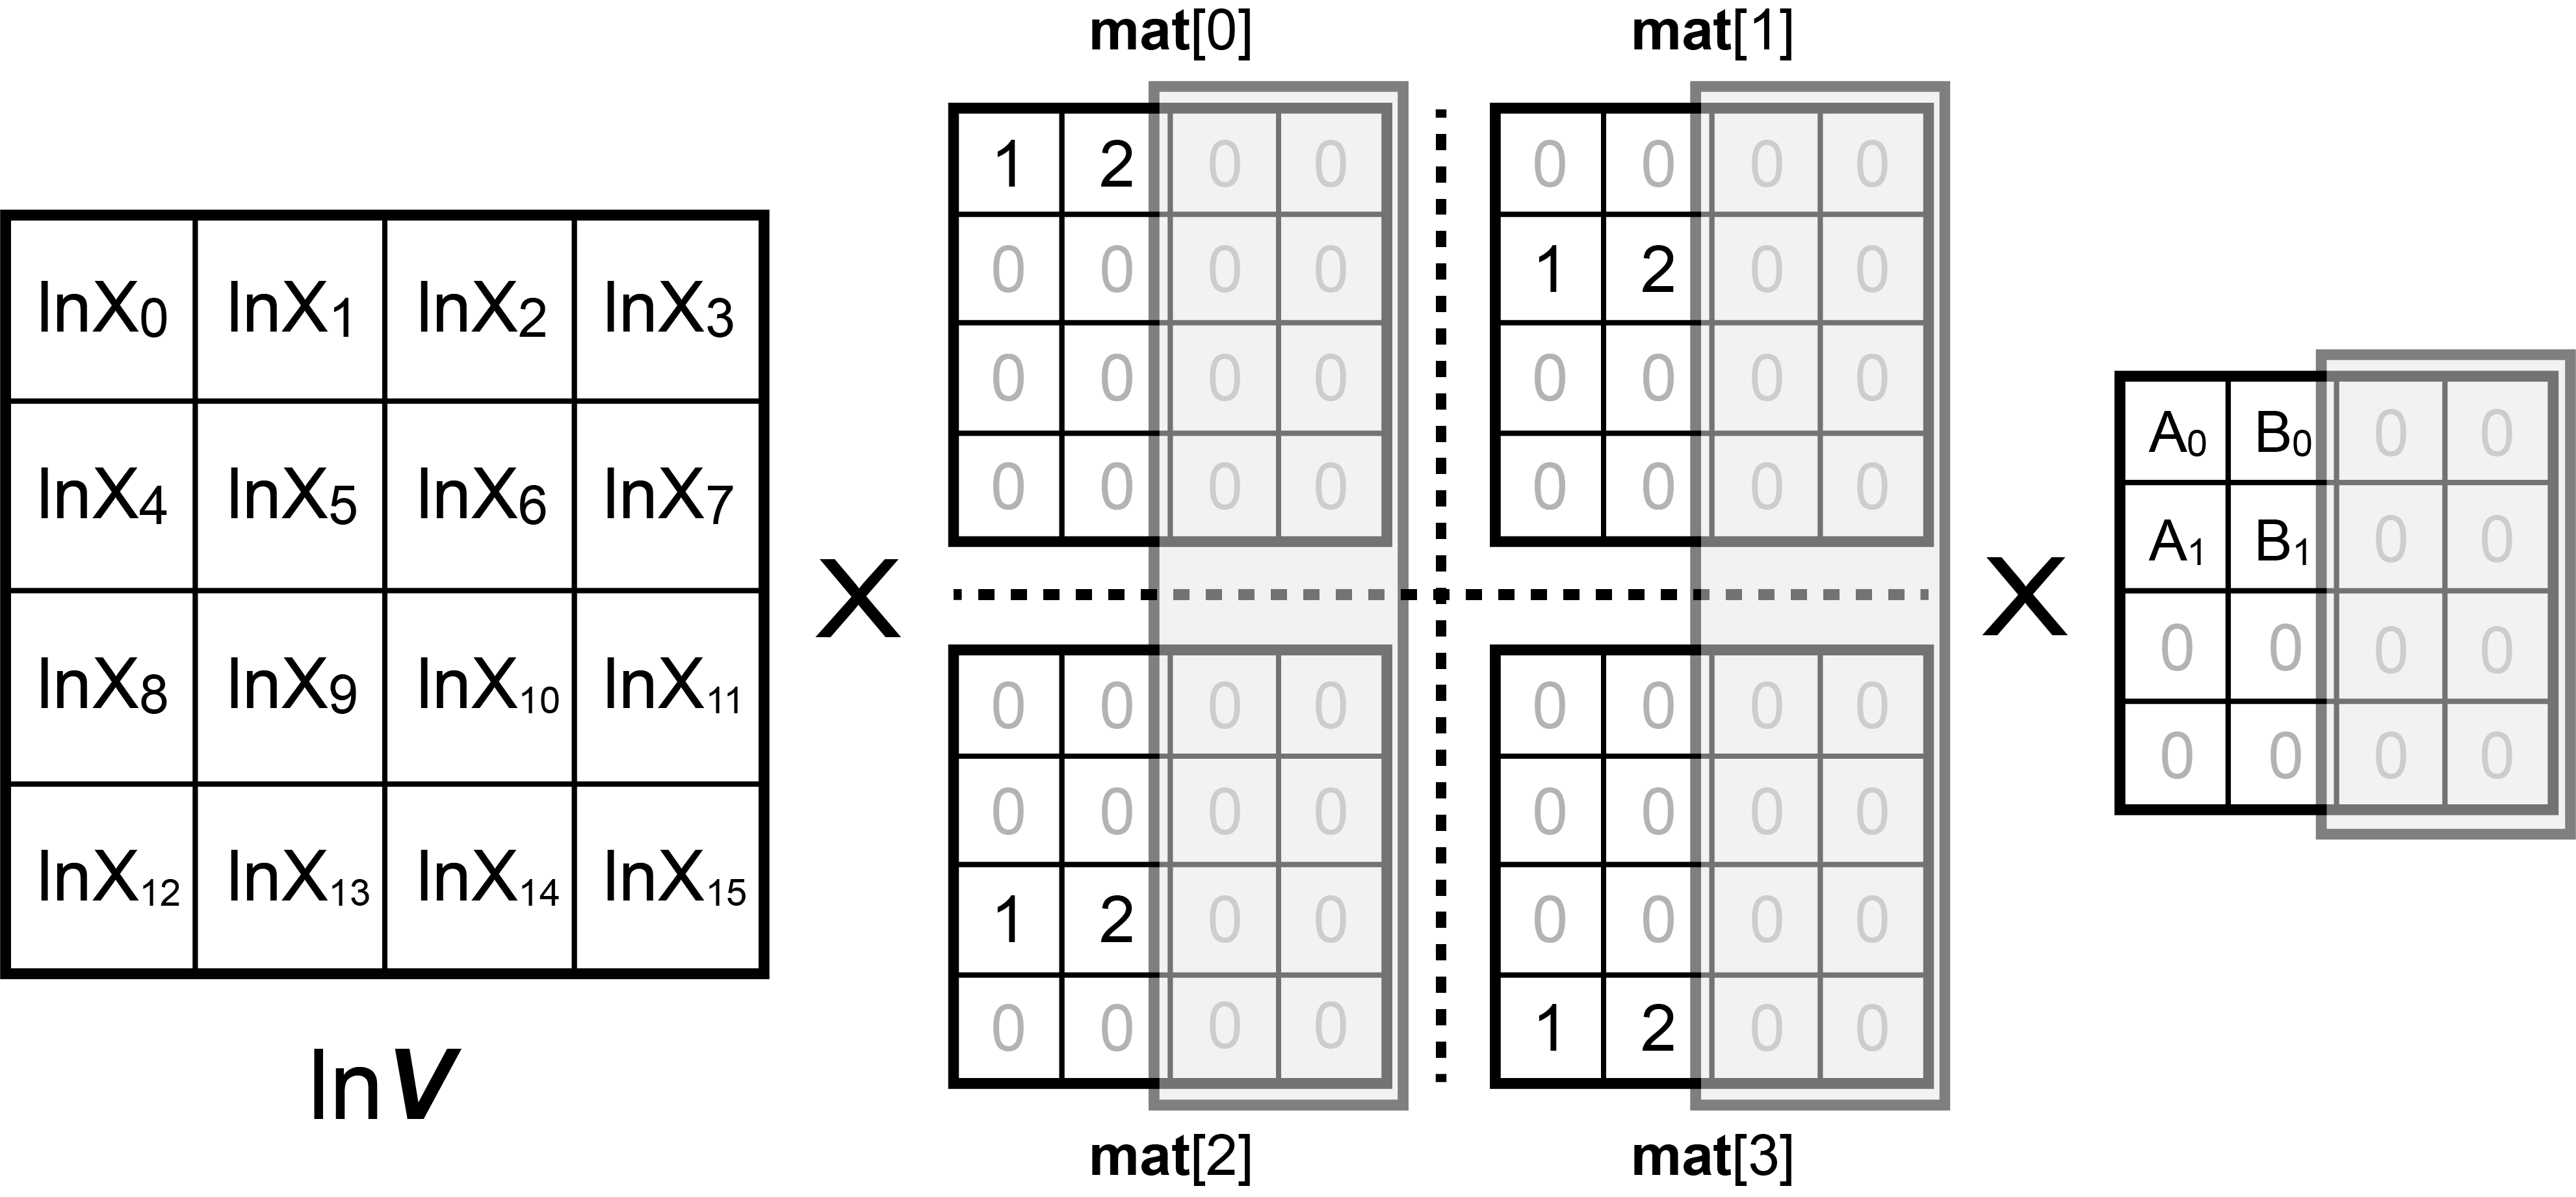
\includegraphics[scale=0.35]{figures/problem.png}}
    \caption{An example where $s = 4, k = 2, j = 2$ with naive Cube-$f(x)$}
    \label{fig:problem}
    \end{figure}

Since incrementing the Taylor series's order does not increase the evaluation precision significantly in most cases, the order requirement is not too high, which means the order number does not have to equal the slide length of the Matrix MACs. Fig. \ref{fig:problem} shows a naive application of Cube-$f(x)$ where the order number is two, the side length is four, and the evaluated function number is two. In this case, we can easily observe that half of the Matrix MAC units we shade are full of zeros in the preparation and computation stages. Since all the units of the Matrix MACs must be utilized in each step of the matrix multiplication, the shaded units' computation power is wasted, which generates meaningless zero results.

\begin{figure}[t]
    \centering{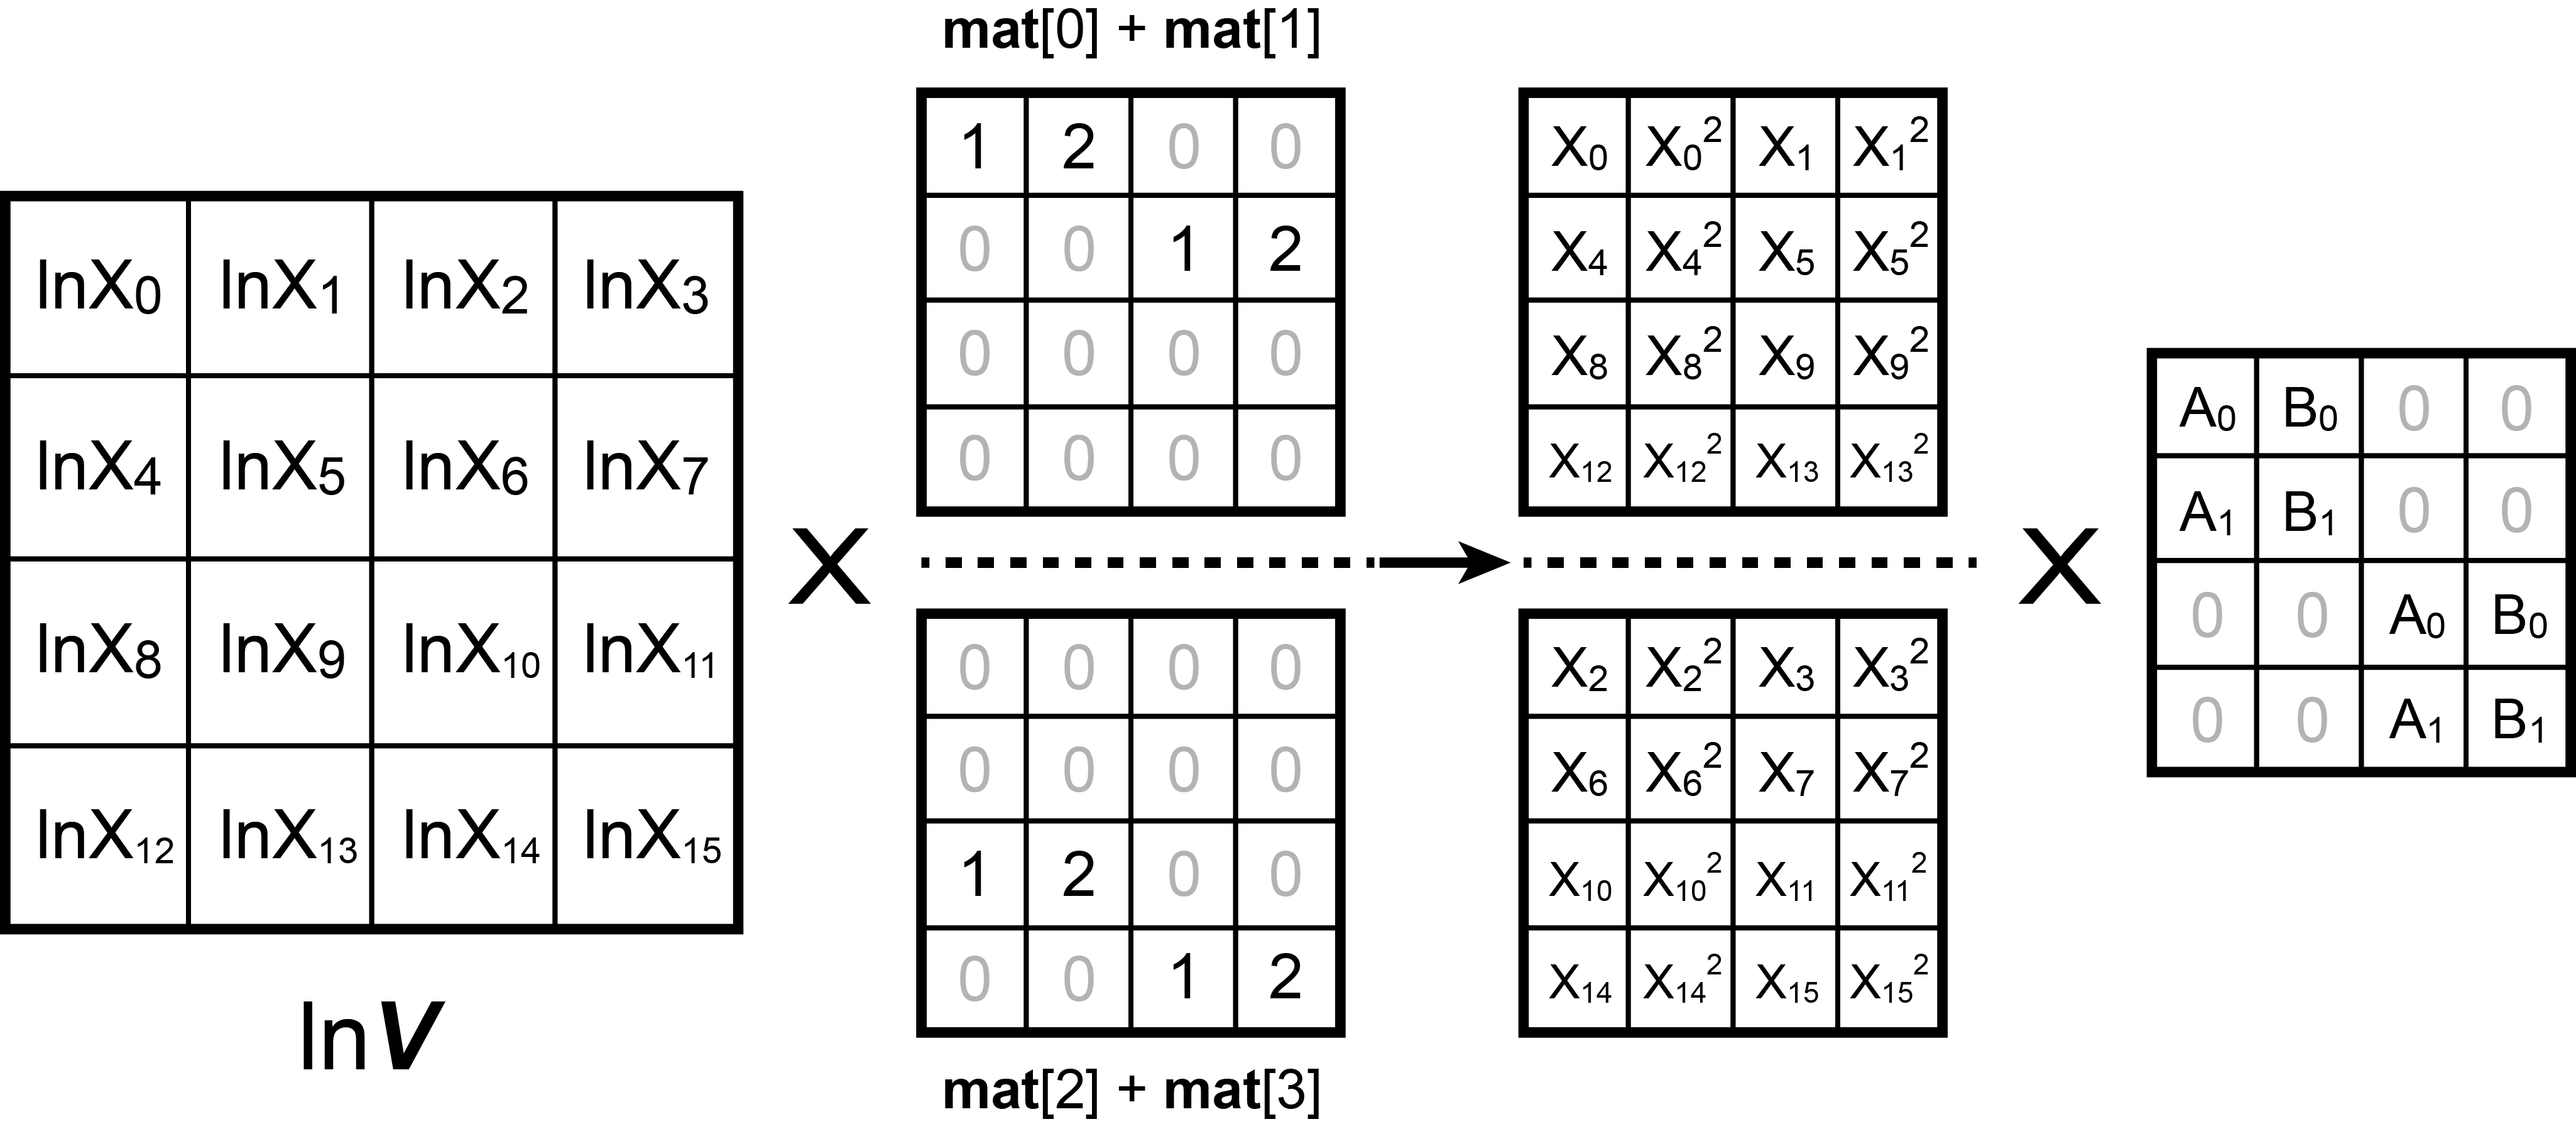
\includegraphics[scale=0.35]{figures/parallel.png}}
    \caption{An example where $s = 4, k = 2, j = 2$ with In-matrix Parallelism}
    \label{fig:parallel}
    \end{figure}

To avoid the computation power waste, we propose In-Matrix Parallelism, which merges multiple matrices and Cube-$f(x)$ loop steps. As shown in Fig. \ref{fig:parallel}, in the preparation stage, the Sequence Matrix $mat[0]$ and $mat[1]$ are merged into one single Sequence Matrix $mat[0] + mat[1]$, where the two non-zero columns of $mat[1]$ are moved to the third and fourth column of the $mat[0]$. Therefore, the result Variable Sequence matrix is a combination of the columns of the two related result matrices. Similarly, to fit the Variable Sequence matrix generated in the preparation stage, the Coefficient Matrix also combines the two original Coefficient Matrices but combines the rows of the matrices instead of the columns in the computation stage. As a result, all the elements of the result matrix are non-zero and valid, which means no computation power is wasted to compute zeros. Furthermore, the step number of the main loop is decreased to two, and the Matrix MAC Count is cut from eight to four, significantly reducing the execution time.

\begin{figure}[t]
    \centering{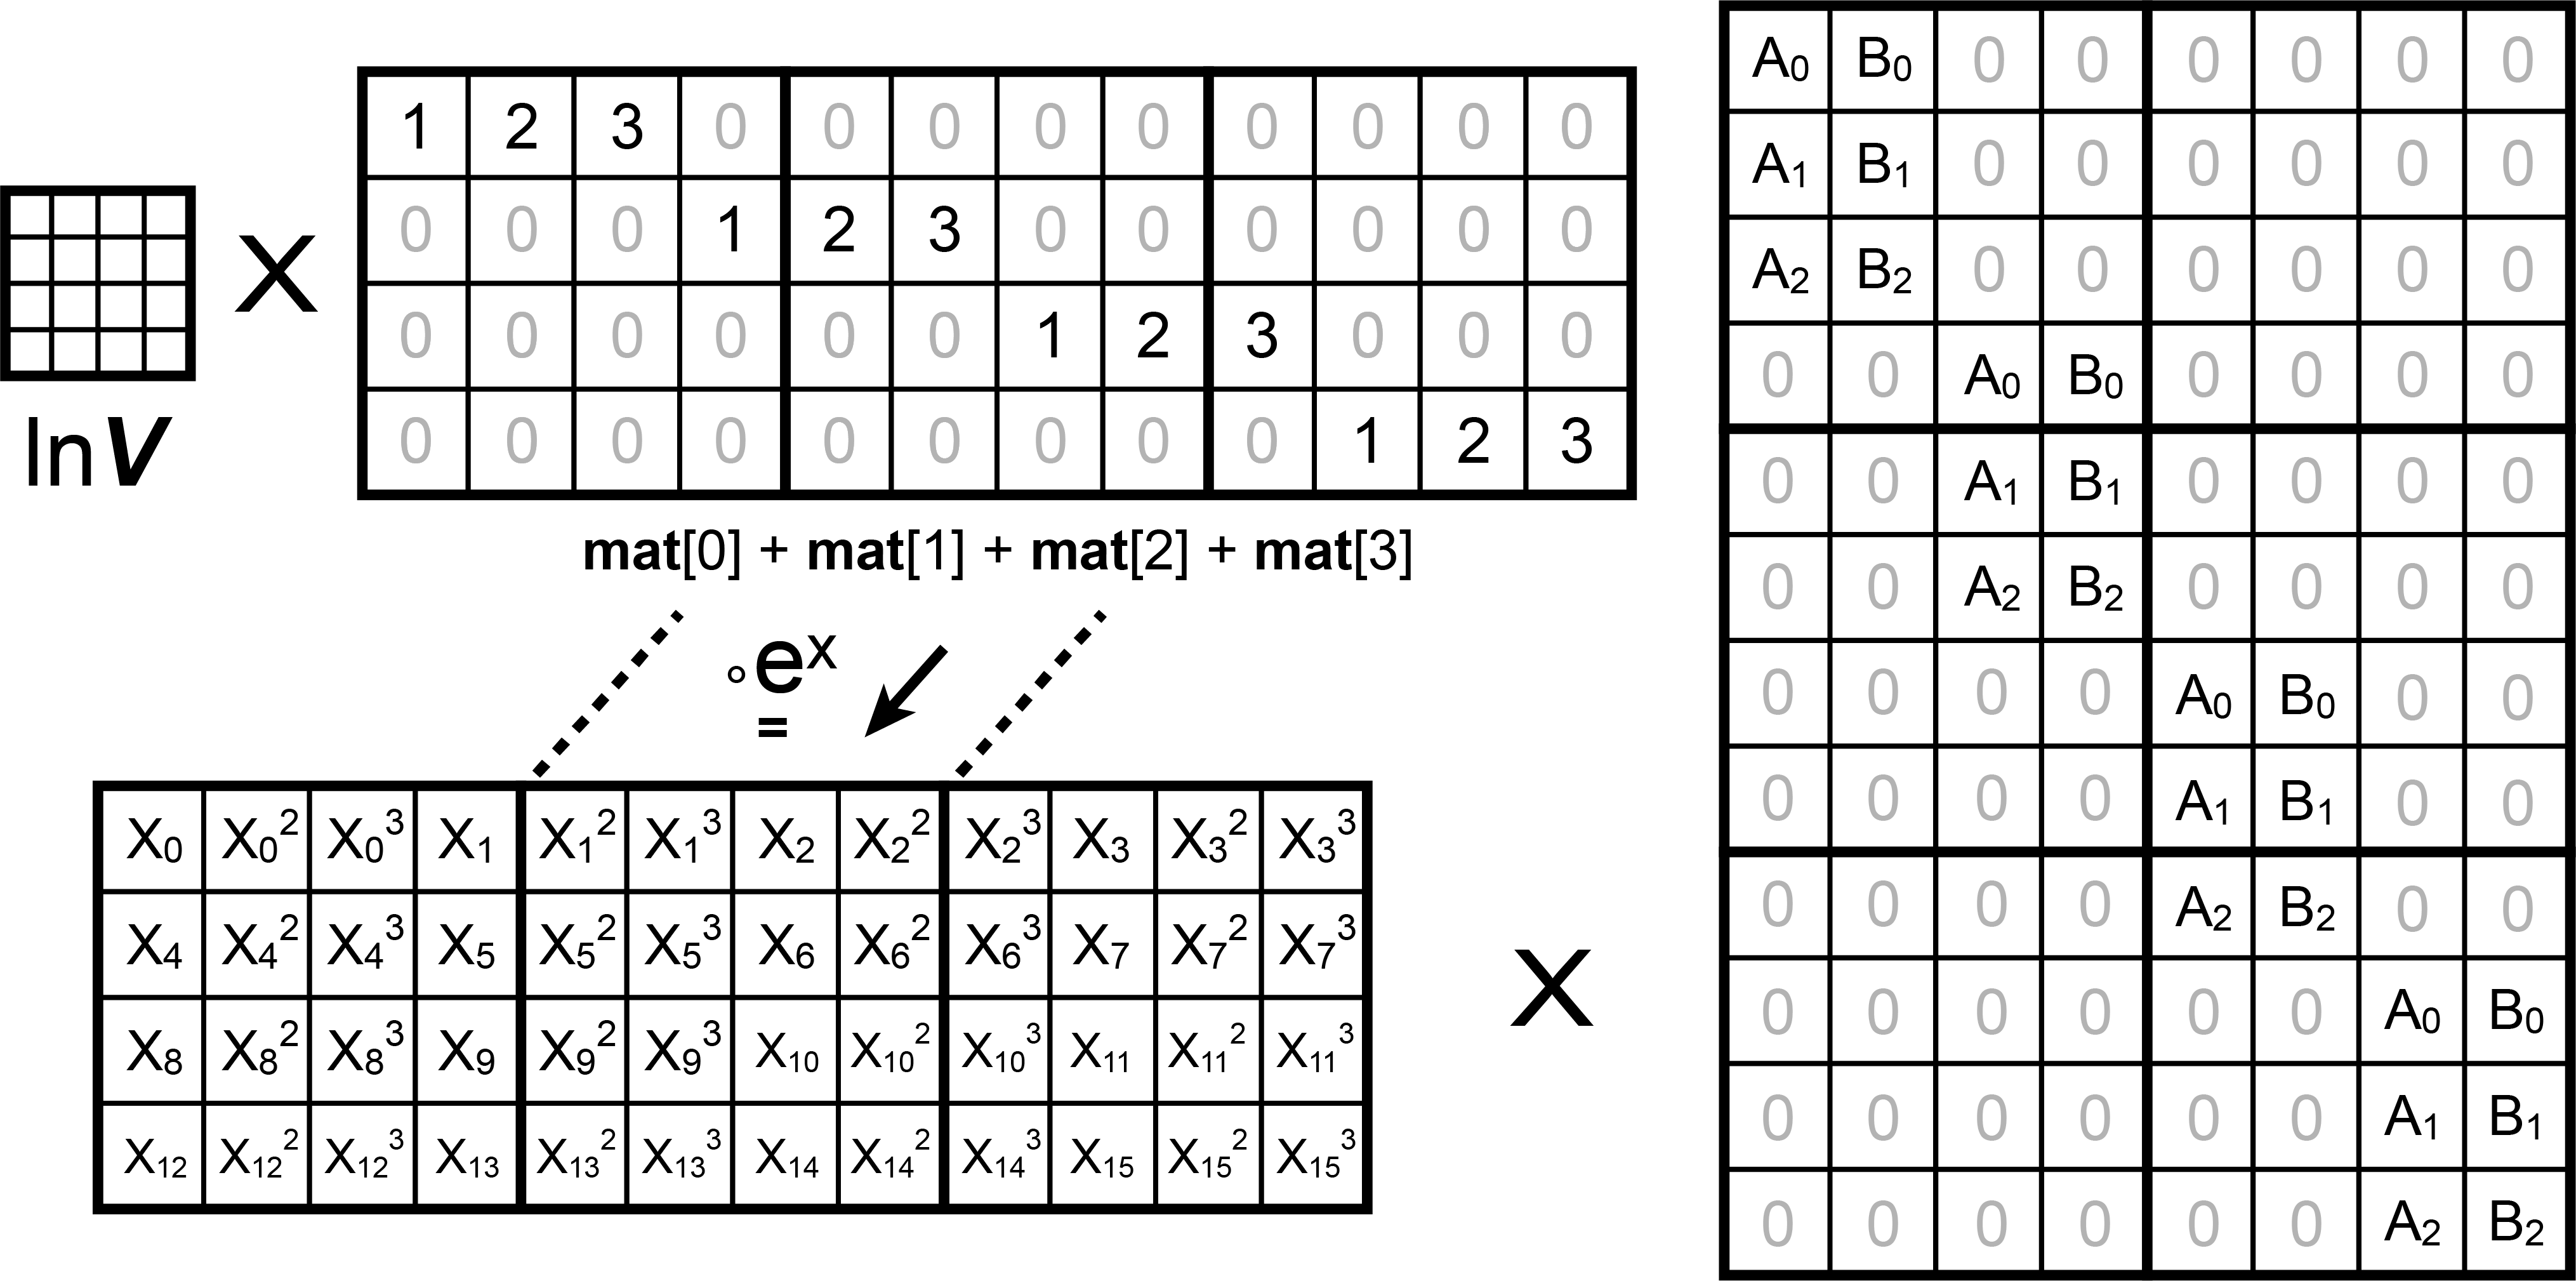
\includegraphics[scale=0.35]{figures/parallel_1.png}}
    \caption{An example where $s = 4, k = 3, j = 2$ with In-matrix Parallelism}
    \label{fig:parallel_1}
    \end{figure}

However, In-matrix Parallelism cannot always improve the efficiency of Cube-$f(x)$. As the example given in Fig. \ref{fig:parallel_1}, we increase the order number to three. Then, in the preparation stage, one Matrix MAC, whose side length is four, cannot simultaneously contain six non-zero columns of two Sequence Matrices. Therefore, to fully utilize the computation power, we can only fuse four original Sequence Matrices into three basic units of the Matrix MACs, whose total column number is 12. Since the matrices of a matrix multiplication should share the same $k$-dimension, the Coefficients Matrix must be a combination of six matrices in the computation stage, whose row number is 12. The Matrix MAC Count of Cube-$f(x)$ with In-matrix Parallelism increases to $(3 + 3 \times 2 = 9)$ compared to $(4 + 4 = 8)$ with naive Cube-$f(x)$. Hence, in this case, In-matrix Parallelism does not decrease the Matrix MAC Count but increases a lot instead. Therefore, in the following subsection, we analyze and quantify when In-matrix Parallelism improves the performance and how to decide the number of merged Sequence Matrices.

\subsection{Quantification \label{sec:qua}}

For a Matrix MAC of the shape $(s \times s)$, let us consider an application of Cube-$f(x)$, where the Taylor polynomial order number is $k$, the evaluated function number is $j$, and the input data length is $(s \times s)$. 

\begin{figure}[t]
    \centering{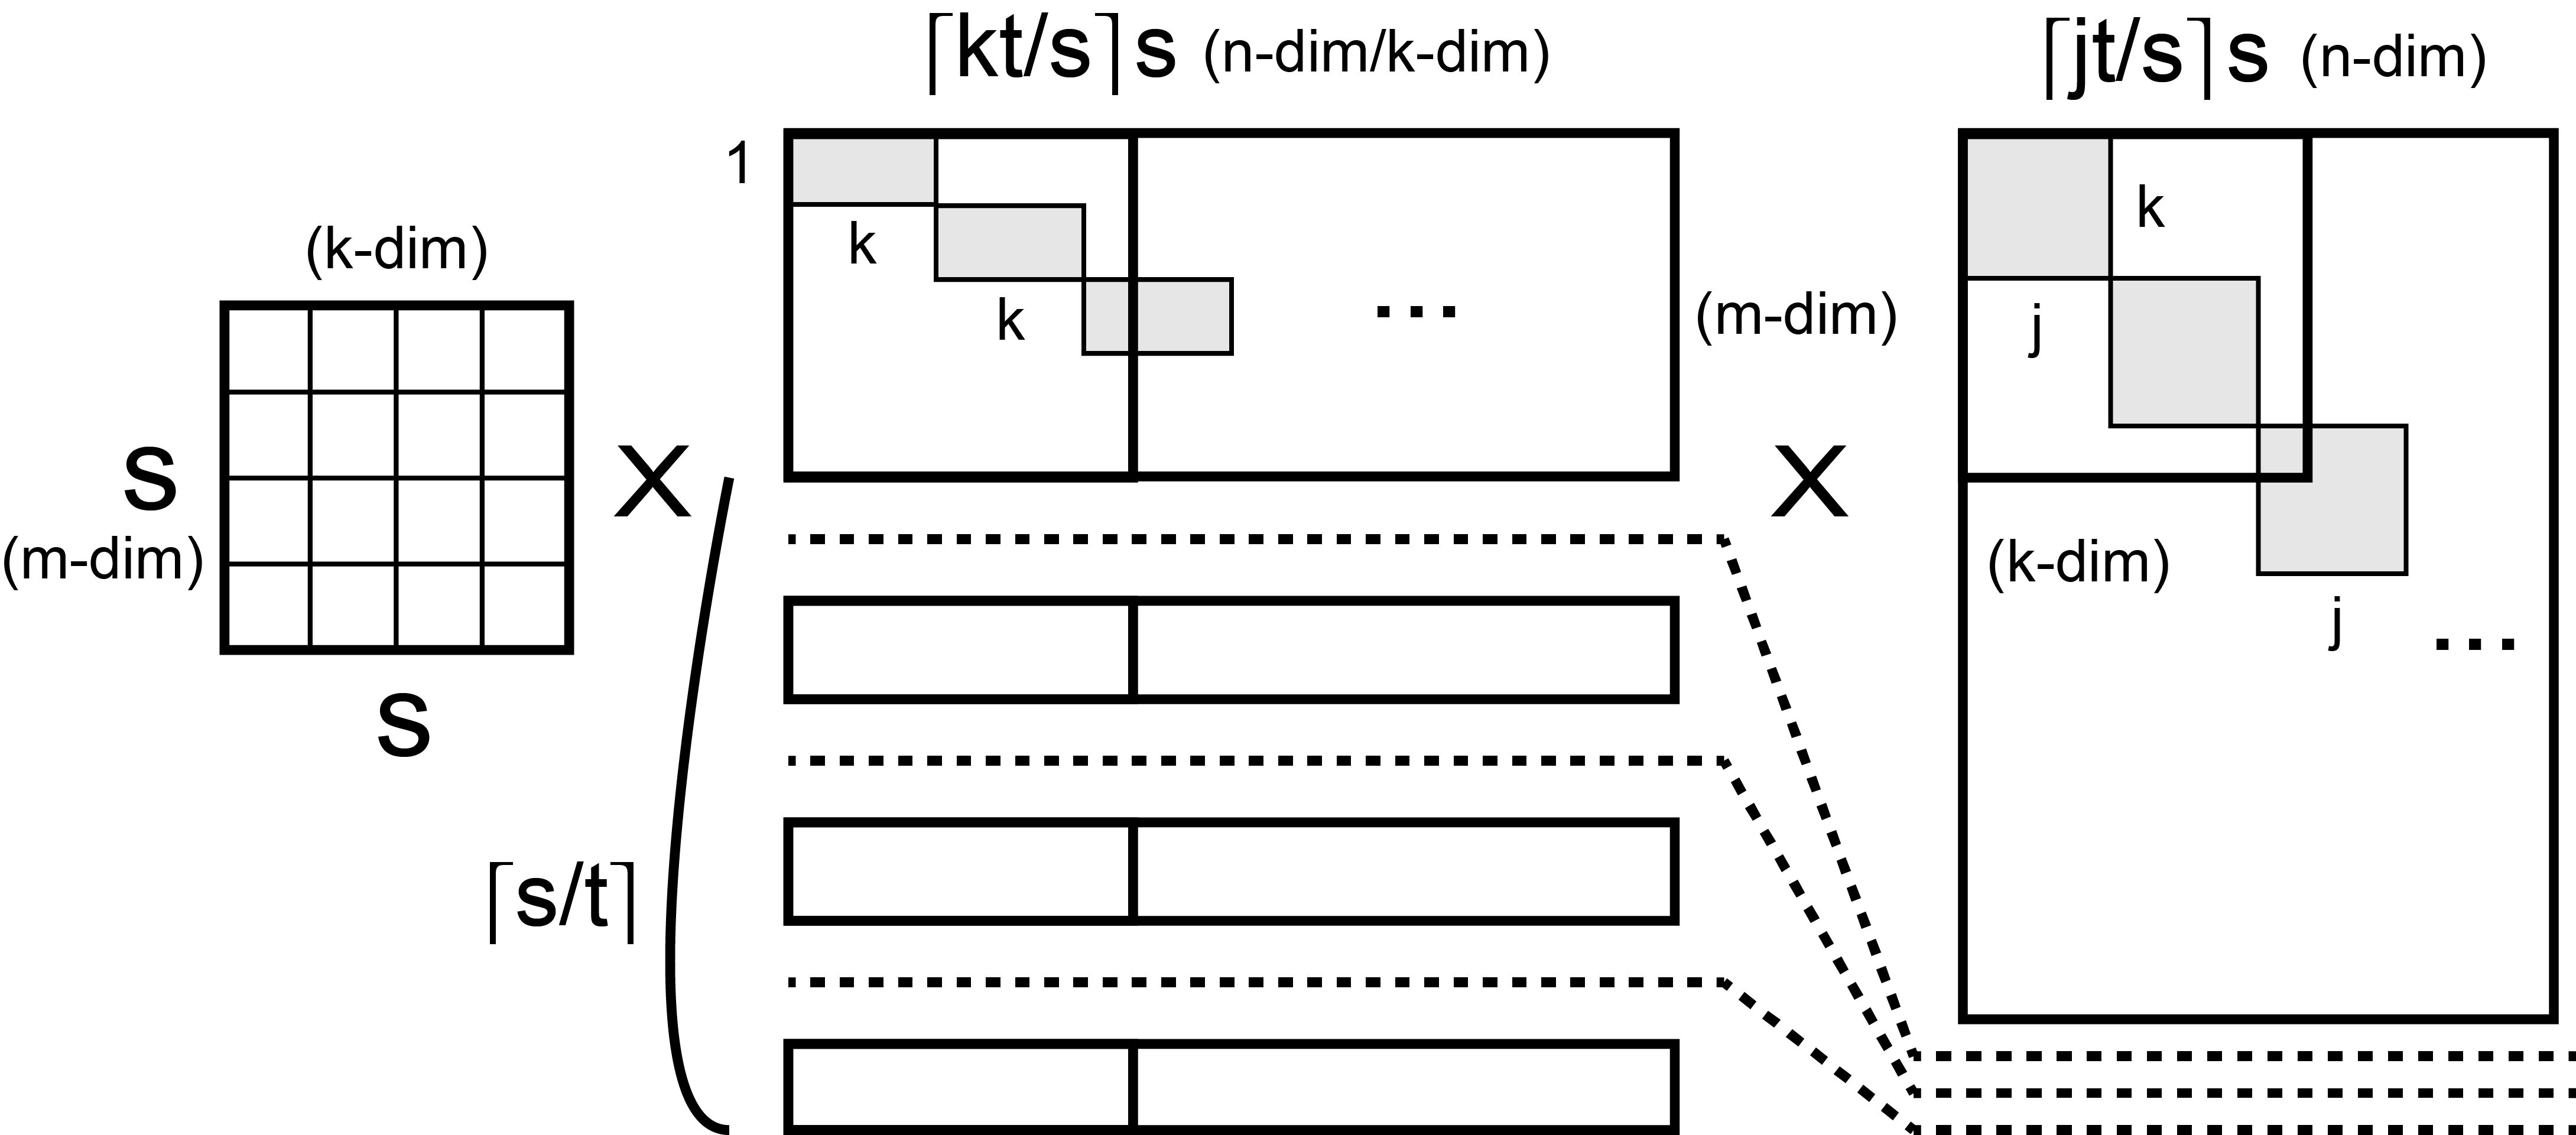
\includegraphics[scale=0.35]{figures/general.png}}
    \caption{Cube-$f(x)$ with In-matrix Parallelism for General Cases}
    \label{fig:general}
    \end{figure}

In the preparation stage, since the order number is $k$, the shape of the non-zero data from each original Sequence Matrix is $(1 \times k)$. Let us merge $t$ original Sequence Matrices, as shown in Fig. \ref{fig:general}, where $t \in \mathbb{N}^{+}, 1 \le t \le s$. Then, the loop step of Cube-$f(x)$ is:

\begin{equation}
    \label{eq:gen_1}
    \begin{aligned}
    L = \ceil*{\frac{s}{t}}
    \end{aligned}
    \end{equation}

where $\ceil*{x}$ is the ceiling function. And the $n$-dimension of the matrix multiplication is:

\begin{equation}
    \label{eq:gen_2}
    \begin{aligned}
    D_{p_n} = \ceil*{\frac{kt}{s}} \cdot s
    \end{aligned}
    \end{equation}

Hence, the Matrix MAC Count of the preparation stage for one loop step is:

\begin{equation}
    \label{eq:gen_3}
    \begin{aligned}
    M_{p} = \ceil*{\frac{kt}{s}} \cdot s \cdot \frac{s^2}{s^3} = \ceil*{\frac{kt}{s}}
    \end{aligned}
    \end{equation}

Similarly, in the computation stage, the Coefficient Matrix is merged by $t$ original Coefficient Matrices. Therefore, the $n$-dimension of the matrix multiplication is:

\begin{equation}
    \label{eq:gen_4}
    \begin{aligned}
    D_{C_n} = \ceil*{\frac{jt}{s}} \cdot s
    \end{aligned}
    \end{equation}

Since the $k$-dimension of the matrix multiplication equals the $n$-dimension in the preparation stage's matrix multiplication, the Matrix MAC Count of the computation stage for one loop step is:

\begin{equation}
    \label{eq:gen_5}
    \begin{aligned}
    M_c = \ceil*{\frac{jt}{s}} \cdot \ceil*{\frac{kt}{s}} \cdot s^2 \cdot \frac{s}{s^3} = \ceil*{\frac{jt}{s}} \cdot \ceil*{\frac{kt}{s}}
    \end{aligned}
    \end{equation}

Hence, the Matrix MAC Count of Cube-$f(x)$ with In-Matrix Parallelism for $L$ steps is:

\begin{equation}
    \label{eq:gen_6}
    \begin{aligned}
    M &= L \cdot (M_p + M_c)  \\
      &= \ceil*{\frac{s}{t}} \cdot \ceil*{\frac{kt}{s}} \cdot (1 + \ceil*{\frac{jt}{s}})
    \end{aligned}
    \end{equation}

Formally, we formulate an optimization problem:

\begin{equation}
    \label{eq:optimized_2}
    \begin{aligned}
        min\quad &M = \ceil*{\frac{s}{t}} \cdot \ceil*{\frac{kt}{s}} \cdot (1 + \ceil*{\frac{jt}{s}}) \\
        s.t.\quad &t \in \mathbb{N}^{+}, 1 \le t \le s
    \end{aligned}
\end{equation}

\begin{table*}[tbp]
    \begin{adjustbox}{addcode={
        \begin{minipage}{\width}}{
            \label{tab:precison}
            \caption{Precision Evaluation for Data Type Float16}
        \end{minipage}},rotate=90,center}
        \scalebox{0.7}{
            \begin{tabular}{c|c|c|c|c|c|c|c|c}
            \toprule[1pt]
                \textbf{Function} &
                \textbf{Input} &
                \textbf{Numpy} &
                \makecell[c]{\textbf{CORDIC Err.} \\ \textbf{Iter = 8}} &
                \makecell[c]{\textbf{Horner's Err.} \\ \textbf{Order = 8}} &
                \makecell[c]{\textbf{Cube-f(x) Err.} \\ \textbf{Order = 8}} &
                \makecell[c]{\textbf{CORDIC Err.} \\ \textbf{Iter = 16}} &
                \makecell[c]{\textbf{Horner's Err.} \\ \textbf{Order = 16}} &
                \makecell[c]{\textbf{Cube-f(x) Err.} \\ \textbf{Order = 16}} \\
            \midrule[0.5pt]

            \multirow{3}*{\makecell[c]{sin(x)}} 
            ~ & 0.14 & 0.1395 & 0.000\% & 0.012\% & 0.012\% & 0.000\% & 0.012\% & 0.012\% \\
            ~ & 0.52 & 0.4969 & 0.000\% & 0.011\% & 0.011\% & 0.000\% & 0.011\% & 0.011\% \\
            ~ & 2.08 & 0.8731 & 0.000\% & 0.178\% & 0.178\% & 0.000\% & 0.046\% & 0.046\% \\
            \midrule[0.5pt]

            \multirow{3}*{\makecell[c]{cos(x)}}
            ~ & 0.14 & 0.9902 & 0.000\% & 0.002\% & 0.002\% & 0.000\% & 0.002\% & 0.002\% \\
            ~ & 0.52 & 0.8678 & 0.000\% & 0.017\% & 0.017\% & 0.000\% & 0.017\% & 0.017\% \\
            ~ & 2.08 & -0.4875 & 0.000\% & 1.917\% & 1.917\% & 0.000\% & 0.214\% & 0.214\% \\
            \midrule[0.5pt]

            \multirow{3}*{\makecell[c]{tan(x)}}
            ~ & 0.14 & 0.1409 & 0.000\% & 0.049\% & 0.049\% & 0.000\% & 0.049\% & 0.049\% \\
            ~ & 0.52 & 0.5726 & 0.000\% & 0.052\% & 0.052\% & 0.000\% & 0.034\% & 0.034\% \\
            ~ & 2.08 & -1.791 & 0.000\% & 1,181\% & 1,180\% & 0.000\% & 11,160\% & 11,160\% \\
            \midrule[0.5pt]

            \multirow{3}*{\makecell[c]{tanh(x)}}
            ~ & 0.14 & 0.1391 & 0.000\% & 0.049\% & 0.049\% & 0.000\% & 0.049\% & 0.049\% \\
            ~ & 0.52 & 0.4777 & 0.000\% & 0.017\% & 0.017\% & 0.000\% & 0.017\% & 0.017\% \\
            ~ & 2.08 & 0.9693 & 0.000\% & 597.3\% & 595.3\% & 0.000\% & 5,649 \% & 5,620\% \\
            \midrule[0.5pt]

            \multirow{3}*{\makecell[c]{Sigmoid(x)}}
            ~ & 0.14 & 0.5349 & 0.000\% & 0.040\% & 0.040\% & 0.000\% & 0.040\% & 0.040\% \\
            ~ & 0.52 & 0.6271 & 0.000\% & 0.031\% & 0.031\% & 0.000\% & 0.031\% & 0.031\% \\
            ~ & 2.08 & 0.8889 & 0.000\% & 1.239\% & 1.184\% & 0.000\% & 0.134\% & 0.134\% \\
            \midrule[0.5pt]

            \multirow{3}*{\makecell[c]{GELU(x)}}
            ~ & 0.14 & 0.0778 & - & 0.034\% & 0.034\% & - & 0.049\% & 0.049\% \\
            ~ & 0.52 & 0.3632 & - & 0.021\% & 0.021\% & - & 0.021\% & 0.021\% \\
            ~ & 2.08 & 2.0410 & - & 14.17\% & 14.17\% & - & 0.289\% & 0.194\% \\
            \bottomrule[1pt]

            \end{tabular}
        }
    \end{adjustbox}
    \end{table*}

which is an integer programming (IP) problem. Intuitively, increasing $t$ can decrease the loop step $L$ and raise the $n$-dimention in both the preparation and computation stages. In addition, $M$ in Eq. \ref{eq:optimized_2} is not a differentiable function of $t$. Therefore, to minimize $M$, we must analyze the optimization problem with different parameters case by case. Fortunately, since the problem has a small and finite feasible domain, we can easily find the optimized solution by brute-force searching when given specific parameters, which achieves the best performance of Cube-$f(x)$.

\section{Evaluation \label{sec:5}}

In this section, we evaluate the performance of Cube-$f(x)$ on Huawei Ascend 310 AI processors based on DaVinci architecture \cite{DBLP:conf/hotchips/LiaoTXZ19} in both precision and efficiency. Huawei Ascend 310 has two DaVinci Cores as the essence of the computation, either of which equips a $(16 \times 16, s = 16)$ Matrix MAC to perform the matrix multiplication. Since Cube-$f(x)$ can naturally execute in parallel, we only activate a single DaVinci Core during the evaluation for simplicity. All the experiments given in the evaluation are programmed as DaVinci Kernels with Tensor Boost Engine (TBE) and Tensor Iterator Kernel (TIK) based on a Huawei full-stack programming framework called AI heterogeneous Compute Architecture (CANN) \cite{CANN}. All the experiment results are evaluated from Huawei's official profiler tool, \textit{msprof}, which reports the detailed runtime information of a DaVinci Kernel. The data type we used during the evaluation is FP16, one of the most popular data types in the AI applications.

\subsection{Computation Precision Evaluation}

We first evaluate the computation precision of the Cube-$f(x)$. We use six sample functions with three different inputs, including trigonometric functions and popular activation functions in the neural networks, to compare the precision of Cube-$f(x)$ with the CORDIC and Horner's Method, respectively. The two algorithms based on Taylor polynomials are expanded around $x = 0$. The error rates are calculated as the percentage difference between the output of the algorithm and the output of Numpy, a Python library for scientific computing.

First, CORDIC reports $0.000\%$ error rates in either iteration of 8 or 16, showing extremely high precision. The reason is that CORDIC is accurate to the bit of its iteration number, which is even higher than the precision of FP16. While the CORDIC implementations of $tanh(x)$ and $Sigmoid(x)$ are proposed by former researchers \cite{DBLP:conf/iscas/ChenJLLFLY20}, CORDIC for $GELU(x)$ is still absent, which we do not list in the table. 

The other two algorithms based on Taylor polynomials, including Cube-$f(x)$, report a few higher error rates. Generally, except for the outliners, the average error rates of Cube-$f(x)$ are $1.112\%$ and $0.058\%$ for the order numbers 8 and 16, respectively. For comparison, the average error rates of Horner's Method are $1.115\%$ and $0.063\%$ for the order numbers 8 and 16. As for $tan(x)$ and $tanh(x)$ with the input $2.08$, the high error rates are caused by the fact that $2.08$ is out of the radius of convergence $(-\frac{\pi}{2}, \frac{\pi}{2})$ and diverges.

The evaluation results indicate that Cube-$f(x)$ has comparable or lower error rates than Horner's method for most cases. Although the precision of Cube-$f(x)$ is much lower than CORDIC, the errors are caused by the theoretical limit of Taylor expansion but not Cube-$f(x)$ itself. In other words, compared to the pure multiplications and additions of Horner's method, the logarithm and exponent operations of Cube-$f(x)$ do not bring extra errors to the computation and even reduce the errors for some cases. Therefore, for applications that need very high precision, CORDIC is still the best choice. In cases where Taylor expansion has met the precision requirements, Cube-$f(x)$ would be safe to replace other implementations, including Horner's Method.

\begin{figure}[htbp]
    \begin{adjustbox}{addcode={
        \begin{minipage}{\width}}{
            \caption{The execution time evaluation results among four algorithms with the order number of 16}
            \label{fig:compare}
        \end{minipage}},rotate=90,center}
        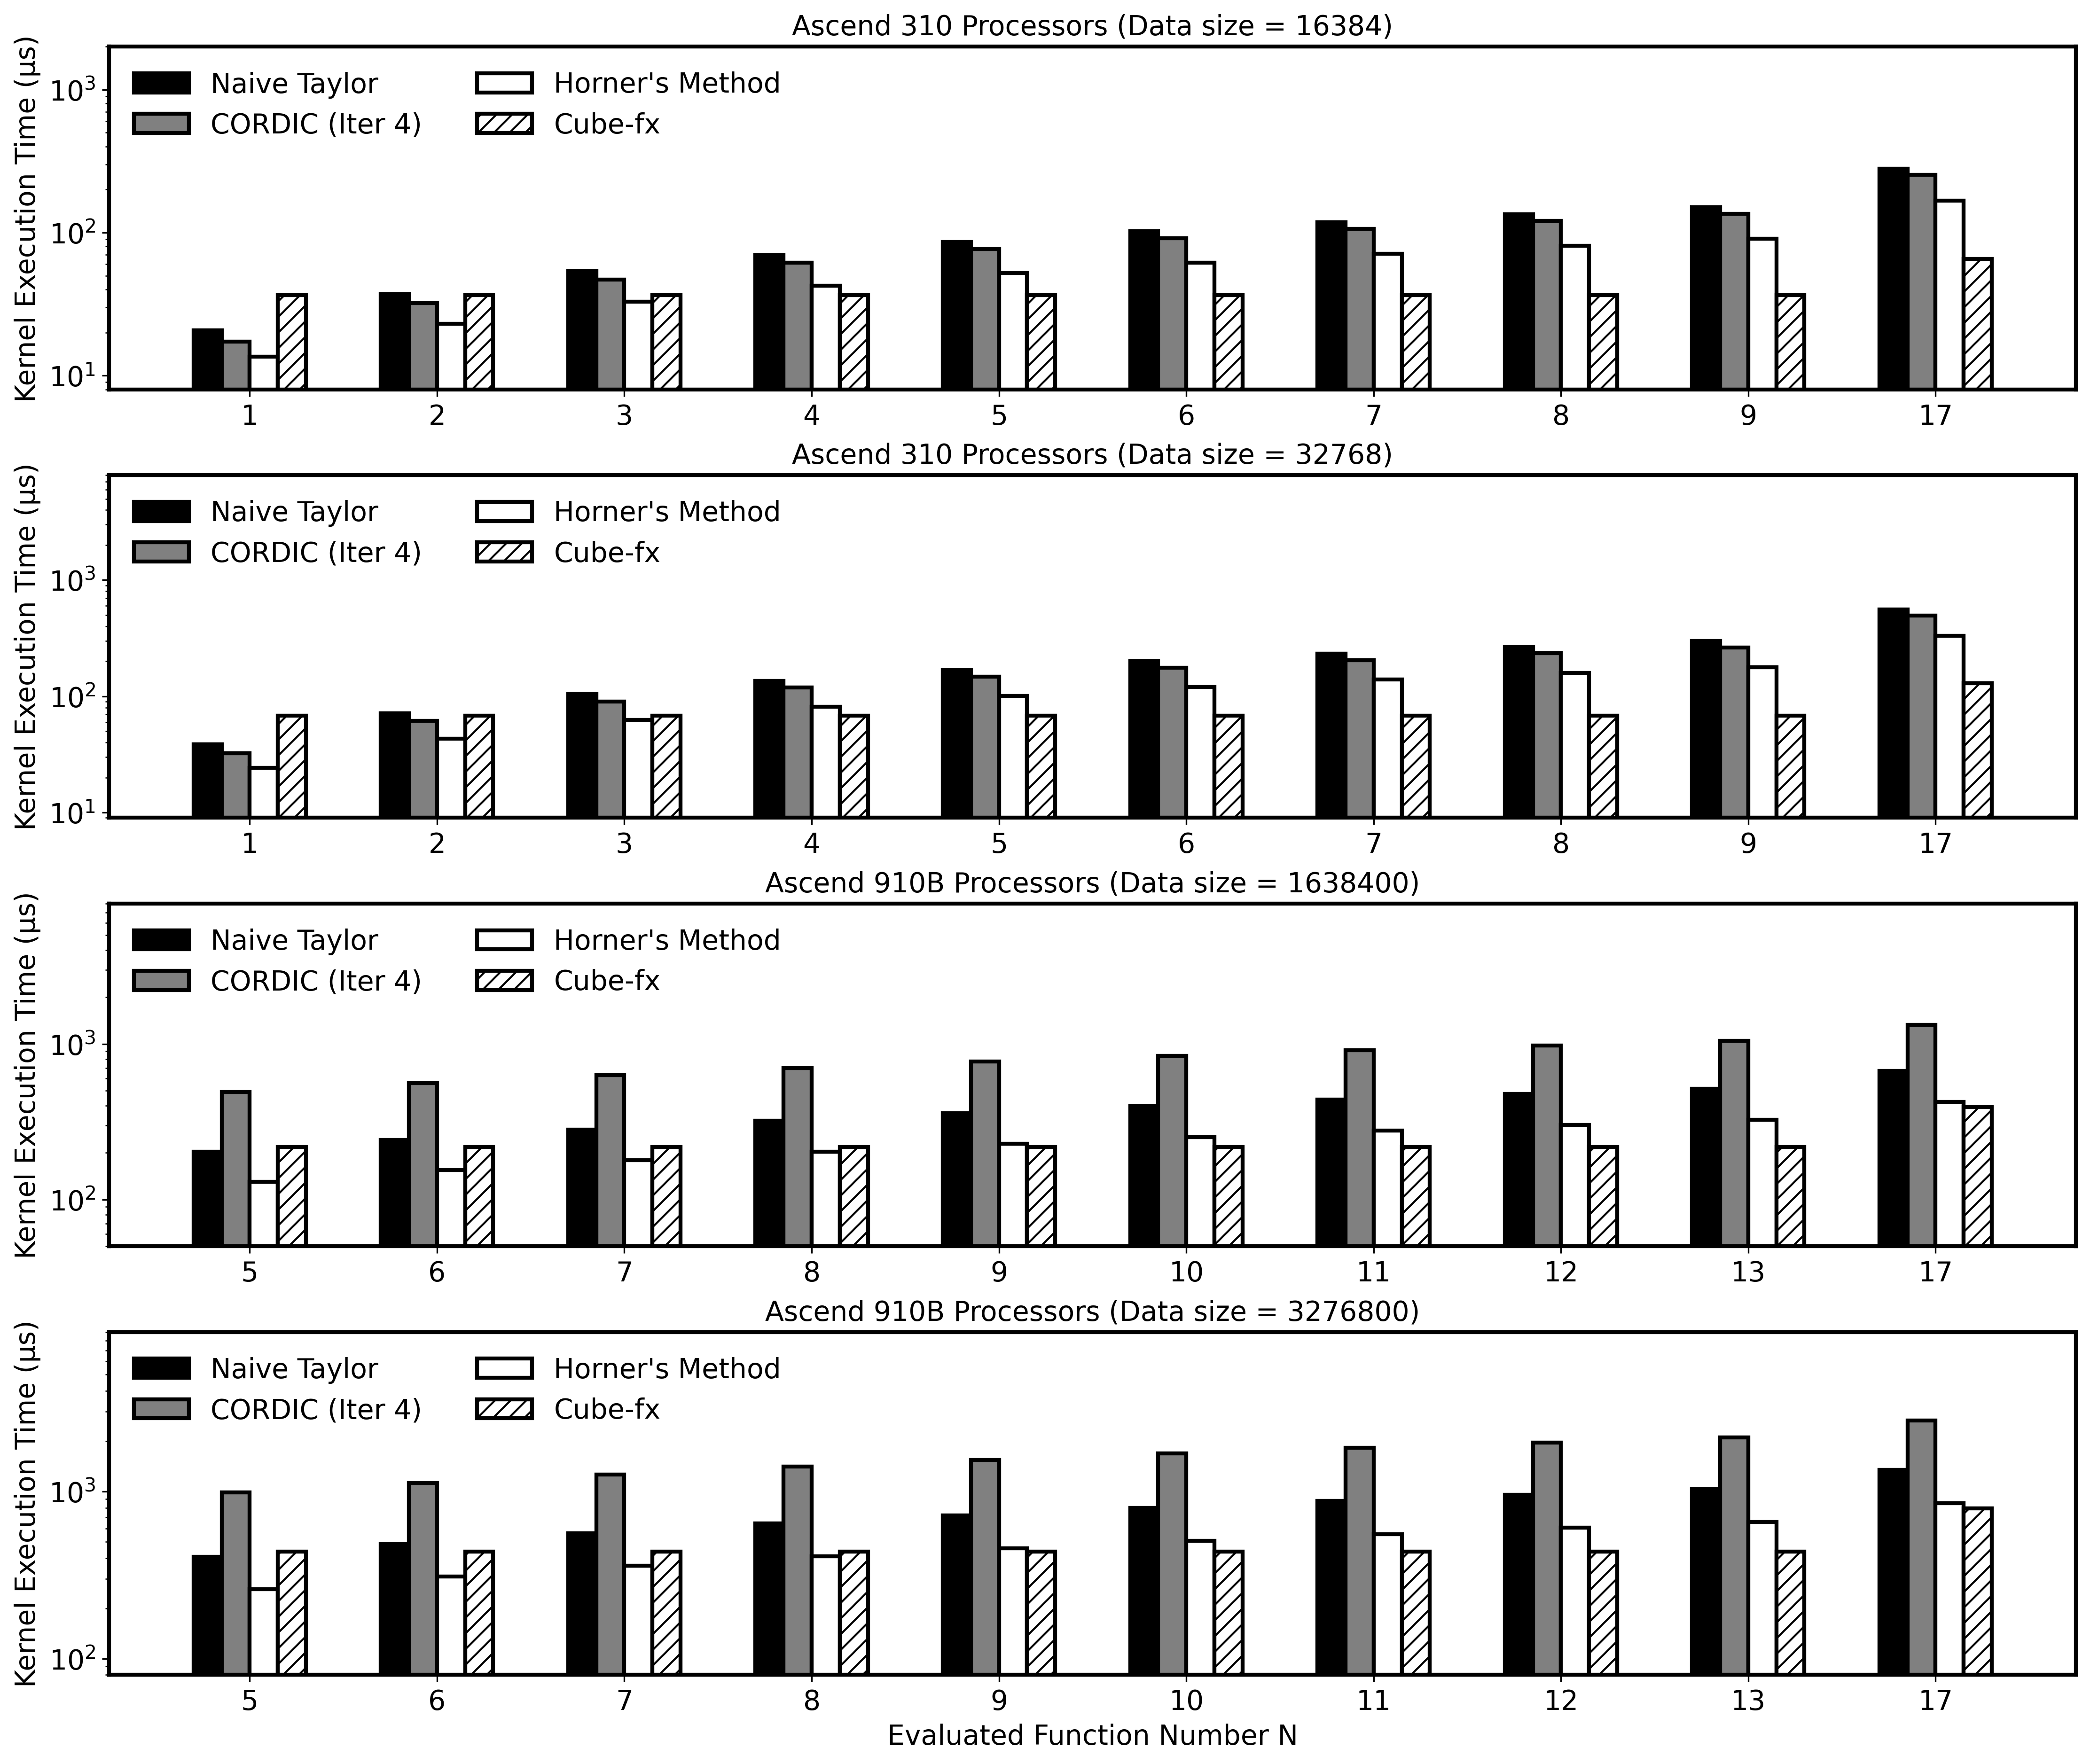
\includegraphics[scale=0.5]{figures/compare.png}
    \end{adjustbox}
\end{figure}

\subsection{Full Matrix MAC Evaluation \label{Sec: 4.2}}

In this subsection, we compare the execution time of Cube-$f(x)$ with naive Taylor expansion implementation, CORDIC, and Horner's Method. The naive Taylor expansion implementation is simply building the Variable Sequences and doing the multiplications with the Taylor polynomial's coefficients based on the vectorized operations. For those algorithms based on Taylor expansion, the order number we used is 16, which equals the side length of the Matrix MACs $(k = s = 16)$ and saturates the Matrix MACs in Cube-$f(x)$. For CORDIC, the iteration number we used is 10, which equals the fraction bit number of FP16. For a fair comparison, all the evaluated functions used here are trigonometric functions to avoid extra data preprocess needed by CORDIC. We analyze the kernel execution time with the variation of the number of the evaluated functions for data sizes 16384 and 32768 respectively.

Fig. \ref{fig:compare} illustrates the evaluation results. Generally, all the algorithms grow with the increment of the evaluated function number, and Cube-$f(x)$ shows significant speedups compared to other implementations. For the case where the data size is 16384, Cube-$f(x)$ shows an average result of $2.68\times$ speedup compared to the naive Taylor expansion implementation, $5.99\times$ speedup compared to CORDIC, and $1.62\times$ speedup compared to Horner's Method. As for the data size of 32768, the speedup results are $2.79\times$ compared to the naive Taylor expansion implementation, $6.12\times$ compared to CORDIC, and $1.66\times$ compared to Horner's Method. 

When the evaluation function number is $1$, Horner's Method is $2.68\times$ and $2.82\times$ faster than Cube-$f(x)$. However, when the number is $9$, Cube-$f(x)$ reversely reports $2.48\times$ and $2.60\times$ speedup instead. In detail, as shown in Fig. \ref{fig:compare}, when the evaluation function number is larger than 3, Cube-$f(x)$ reports better efficiency than other implementations and keeps enlarging the performance gap. The main reason for the results is that compared to the time complexity we discussed in Sec. \ref{sec:3} for naive Cube-$f(x)$, the time complexity of general Cube-$f(x)$ is $O(Nk + \ceil{N / s} \ceil{k / s} + \ceil{N / s} \ceil{k / s} \ceil{j / s})$, where the execution time of Cube-$f(x)$ increases every $s$ evaluated functions. The ceiling functions are added here because the Matrix MAC must complete a basic unit $(s \times s \times s)$ of matrix multiplication each time, as mentioned in Sec. \ref{sec:qua}. Therefore, for the number of evaluated functions within $[1, 16]$, Cube-$f(x)$ reports a nearly constant execution time, while the other implementations increase linearly. As for the evaluated function number of 17, where $\ceil{17 / 16} = 2$, the execution time of Cube-$f(x)$ finally increases to $179.14\%$ of the previous results with the data size of 16384, which reports $4.60\times$ speedup compared to Horner's Method. 

In summary, although Cube-$f(x)$ shows less performance when the evaluation function number is low, it performs with much higher efficiency than other implementations for a high evaluation function number, which is also the situation we focus on in this paper.

\begin{figure}[htbp]
    \begin{adjustbox}{addcode={
        \begin{minipage}{\width}}{
            \caption{The accelerations of In-Matrix Parallelism compared to naive Cube-f(x) and Horner's Method for different order numbers}
            \label{fig:results}
        \end{minipage}},rotate=90,center}
        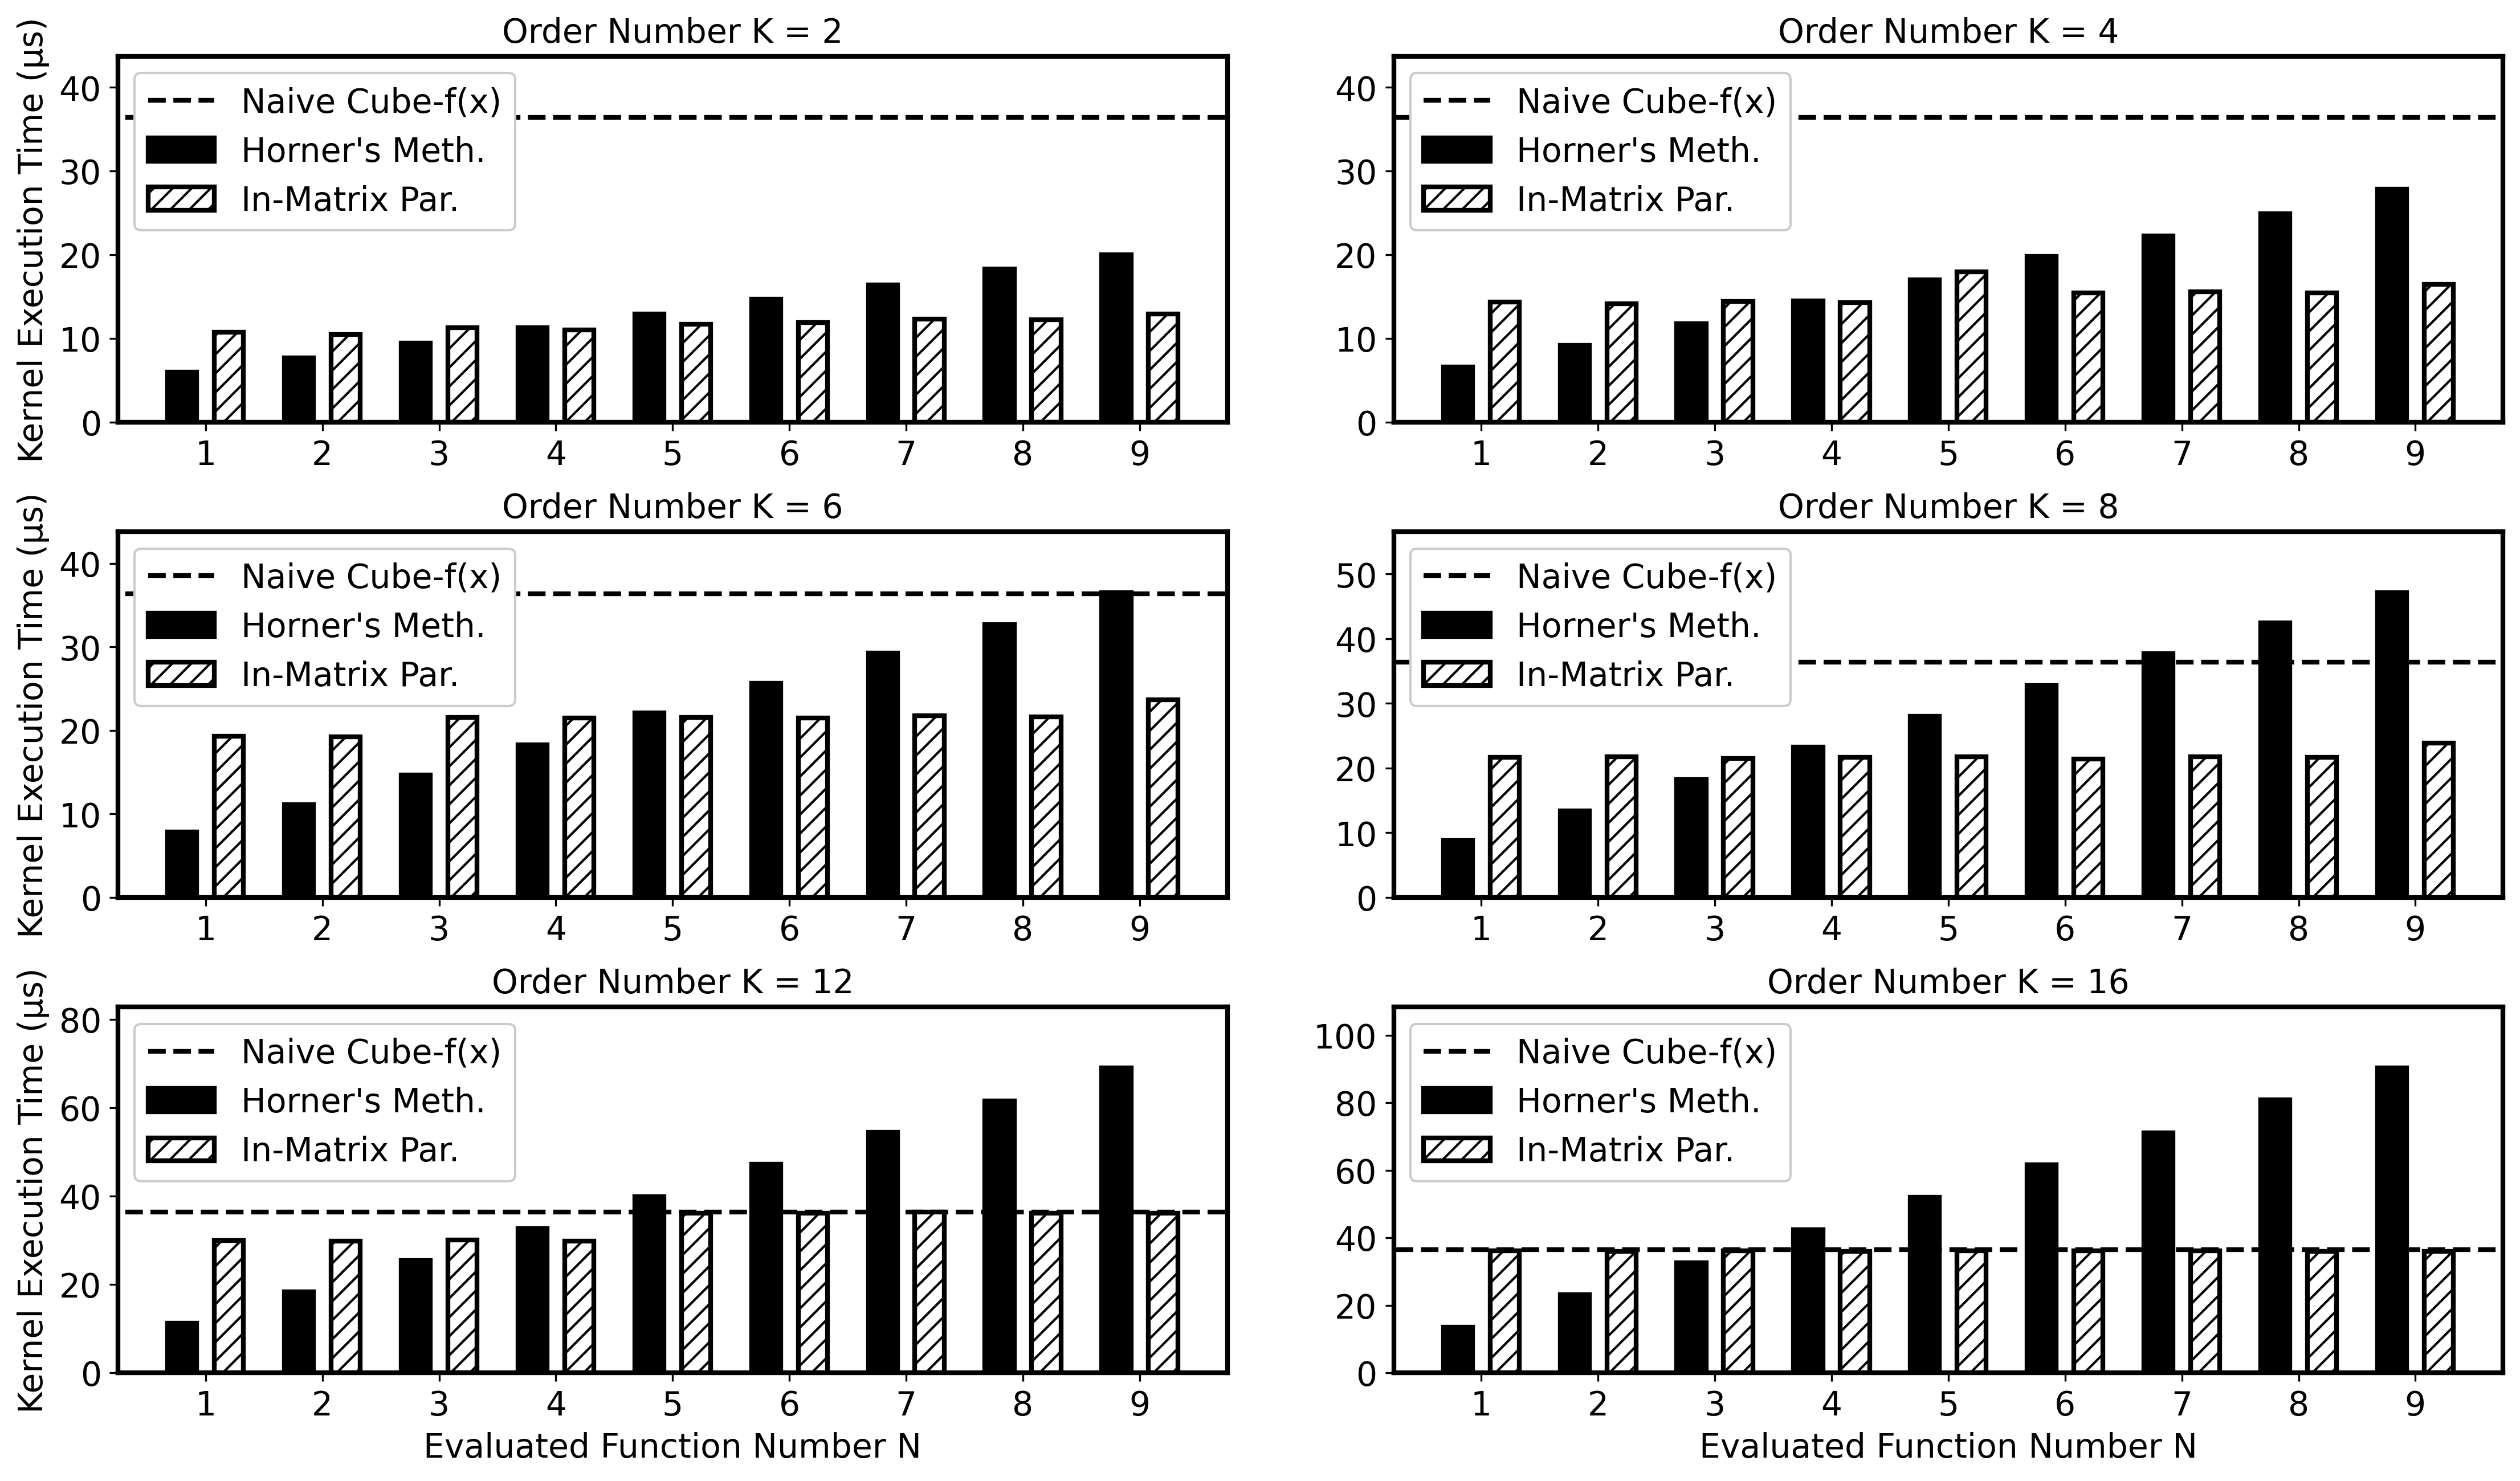
\includegraphics[scale=0.5]{figures/results.png}
    \end{adjustbox}
\end{figure}

\subsection{Unfilled Matrix MAC Evaluation}

This subsection evaluates the performance of Cube-$f(x)$ with In-Matrix Parallelism, where $k = \{2, 4, 6, 8, 12, 16\}$. To indicate the performance improvement of Cube-$f(x)$ with In-Matrix Parallelism, we compare its execution time with those of Horner's Method and naive Cube-$f(x)$. The data size used in this subsection is 16384. Since the on-core memory of Ascend 310 AI processor is limited, our implementation of Cube-$f(x)$ with In-Matrix Parallelism contains a basic tiling strategy of matrix multiplications, which always divides the left matrix along $m$-dimension.

Fig. \ref{fig:results} illustrates our collected evaluation results. Since the execution time of naive Cube-$f(x)$ for all cases is the same, we plot it as a dashed line in all charts, which reports significant performance gaps between other two implementations in most cases. Generally, Cube-$f(x)$ with In-Matrix Parallelism reports an average speedup of $1.83\times$ compared to naive Cube-$f(x)$. While the best case reports $3.39\times$ speedup, the worst reports an equivalent execution time compared to naive Cube-$f(x)$, which means applying In-Matrix Parallelism to Cube-$f(x)$ for all cases is riskless. We further add the execution time of Horner's Method with the low order number requirements for comparison. Since the time complexity of Horner's Method is $O(k)$, naive Cube-$f(x)$ shows much worse performance than Horner's Method in most cases. In-Matrix Parallelism empowers Cube-$f(x)$ again and offers the capability to beat Horner's Method. As shown in Fig. \ref{fig:results}, Cube-$f(x)$ with In-Matrix Parallelism reports lower execution time when the number of evaluated functions is larger than about 4, similar results to the full Matrix MAC results in Sec. \ref{Sec: 4.2}. 

Especially, the results of Cube-$f(x)$ with In-Matrix Parallelism in the case $k = 6$ report similar performance to those in the case $k = 8$. The main reason is that the best original Sequence Matrix number $t$ for the two cases is the same. Therefore, even with In-Matrix Parallelism, some computation power of the Matrix MAC is wasted since $16 \mod 6 \neq 0$. The phenomenon suggests that In-Matrix Parallelism still cannot exploit all computation power of the Matrix MAC, which requires a deeper study in the future.

\section{Conclusion \& Future Work \label{sec:8}}

This paper introduced Cube-$f(x)$, a novel algorithm to evaluate special functions with the powerful Matrix MACs of the AI processors. Based on the fact that the AI processors usually equip poor vector units and a piece of data often needs to be computed by multiple functions in real-world applications, Cube-$f(x)$ converts the building and computation of Taylor polynomials to specific matrix multiplications supported by the Matrix MACs. Since the Matrix MACs must complete a fixed shape of matrix multiplication each time, Cube-$f(x)$ wastes a part of the computation power when the order number of the Taylor polynomial is low. Therefore, we propose In-Matrix Parallelism to fuse the matrix multiplications of Cube-$f(x)$, which again empowers Cube-$f(x)$ and exploits the computation power as much as possible. Although the application and performance of Cube-$f(x)$ are still imperfect, we believe our attempt to extend the programmability of the AI processors would inspire more researchers to work on this novel hardware with more valuable results.

In future work, we will study those special matrix multiplications deeper, which may accelerate other important applications for general purposes but not AI applications. We also will look further at In-Matrix Parallelism to see whether it can be applied to all matrix multiplications, significantly improving the Matrix MACs' utilization.


\chapter{Conclusion and Future work}
\label{sec_5}

In this thesis, an integrated optimization design framework is established for orthopedic devices with lattice microstructures. The framework consists of three modulus: lattice microstructure mechanical property homogenization (Chapter~\ref{gauss}), gradient-based topology optimization (Chapter~\ref{femur} and Chapter~\ref{spine}) and lattice configuration reconstruction (Chapter~\ref{recon}). Regarding academic research and orthopedic clinical treatment aspects, the major outcomes are introduced as follows.\\

{\bf Firstly, a versatile lattice microstructure mechanical property homogenization system is established based on data-driven Gaussian process (GP) machine learning model.} In this project, the GP homogenization system is trained with a sample dataset composed by random simple orthotropic lattice microstructures with varied structural anisotropy. The input variables are strut radii in lattice microstructure along different directions, while the output variables are anisotropic stiffness modulus and failure strengths of the microstructure, which are required during optimization iteration.\\

Comparative analysis results reveals that highest prediction accuracy is achieved when independent single-output GP models are established for each output variables. Albeit higher computation cost is required, the error between GP-homogenized output variables and their reference values are largely decreased. For most testing cases, the average prediction error among the concerned mechanical properties are lower than 10\%. Strong positive correlation relationship is observed on predicted and reference output variables. The coefficient of correlation obtained from correlation analysis is close to 1.\\ 

A major advantage of this GP homogenization model is its capability to make immediate and accurate prediction on mechanical properties of orthotropic lattice unit cells with arbitrary structural anisotropy. The analytical kernel of the GP model is not limited to a specific type of lattice unit cell architecture. By appending new input variables and providing abundant training dataset, the GP homogenization model can be used on model with arbitrary lattice interior structure, providing broad support for the optimization design of lattice orthopedic devices.\\

{\bf Secondly, gradient-based optimization frameworks are created for lattice femoral implant and spinal cage corresponding to customized clinical demand.} Maximum global compliance in orthopedic devices is selected as design target, which is commonly regarded as an efficient countermeasure against stress shielding problem happening in post-operative bone tissue. Constraint conditions including structural failure criteria, bone growth stimulation, additive manufacturing capability are applied to satisfy clinical and fabrication requirement. The performance of stress shielding moderation is quantitatively evaluated by resorbed bone mass fraction and stress shielding intensity of post-implantation femur and vertebrae.\\

For lattice femoral implant, the strut radii in orthotropic lattice microstructures in implant optimization domain are selected as design variables. Multi-scale finite element analysis is conducted in each optimization iteration to enhance computation efficiency. The homogenization of constitutive relationship is completed via the GP machine learning model introduced in Chapter~\ref{gauss}. As an environment-interactive design system, the anisotropic design of lattice femoral implant based on MMA algorithm largely moderates the stress shielding in femur head and shaft. Compared to solid implant, uniform-density isotropic implant and graded-density isotropic implant, the optimized graded-density anisotropic implant reduces the resorbed bone mass by 89.5\%, 47.5\% and 39.4\%, indicating its high potential in total hip arthroplasty clinical treatment.\\

For lattice spinal cage, the relative densities of lattice microstructures in spinal cage domain are selected as optimization design variables. MMA algorithm is adopted to redistribute the basis material allocation among lattice unit cells. Four common clinical spine loading conditions, including non-eccentric loading, flexion loading, extension loading and lateral bending, are simulated to comprehensively examine the design efficiency of the proposed algorithm in clinical application. The performance of optimized spinal cages are quantitatively evaluated by two vertebra-related bio-mechanical indicators: resorbed bone mass fraction and stress shielding severity. Evaluation results verify that MMA algorithm contribute to the moderation of stress shielding in post-operative spine. 38\% reduction in resorbed bone mass fraction and 24\% reduction in stress shielding severity are recorded. However, without overshadowing to the overall optimization performance, it is noticed that over-redistribution of vertebra stress happens in some cases, which may lead to bone degeneration and endplate collapse risk in vertebrae.\\

{\bf Thirdly, a series of reconstruction guidance are provided to convert optimal design variables obtained from optimization design to printable lattice device configurations.} Various finite element types including anisotropic hexagonal element, isotropic trigonometrical element and isotropic tetrahedron element are concerned in this chapter. Boundary representation theory is used to re-establish the lattice microstructures in optimization domain. Samples of anisotropic lattice femoral implant configuration and graded-density lattice spinal cage configuration are presented, which can be directly converted to physical orthopedic products ready for clinical use via additive manufacturing technique.\\

Most outcomes in this thesis are obtained from mechanical simulation of implanted femur and spine system, which may not be able to accurately reflect the actual clinical situation in total hip arthroplasty and lumbar inter-body fusion. Laboratory compression test is recommended in the future to verify the optimization design efficacy of graded-density lattice orthopedic devices from the aspect of experiment. The compression tests should be conducted on artificial or cadaveric bones. Metallic femoral implants and spinal cages with different interior designs should be implanted to conduct comparative analysis on their influence on stress condition in bone tissue. Digital image correlation technique is suggested to record the displacement and deformation variation on bone surfaces during experiment, so that the stress shielding moderation performance can be quantitatively evaluated.\\
\newpage
\thispagestyle{empty}
~\\
%===============================================================================
\newpage
\setcounter{page}{1}
\pagenumbering{roman}

\bibliographystyle{unsrt} 
\bibliography{reference}

\end{document}
\endinput









